\documentclass[a4paper,11pt]{article}


\usepackage[utf8]{inputenc} %damit man auch Umlaute eingeben kann
\usepackage[bitstream-charter]{mathdesign} % Charter als Standardschriftart
\usepackage[scaled=.82]{DejaVuSansMono} % DejaVuSansMono als Code-Schriftart
\usepackage[T1]{fontenc} %damit Umlaute bei einer pdf-Suche auch erkannt werden
\usepackage{amsfonts,amsmath} %Verwendung von Mathematik-Schriftarten
\usepackage{graphicx} %für Grafiken der Formate jpg, png, pdf
\usepackage{float} % um Abbildung wirklich genau dort zu platzieren
\usepackage{url} %für die gute Darstellung von Internet-Links
% \usepackage[ngerman]{babel} %deutsches Sprachpaket
\usepackage[ngerman,english]{babel} %deutsches Sprachpaket
\usepackage[round]{natbib} %für vereinfachte:wen/Querverweise
\usepackage{tikz} %für tikz-Grafiken
\usepackage{paracol}
\usepackage{subfigure}
\usepackage{quoting}
\usepackage{pgfplots}
\usepackage{capt-of}
\usepackage{listings} % für Quelltext mit Syntax-Highlighting
\usepackage[colorlinks=true, allcolors=blue]{hyperref}
\usepackage{enumerate}
\setlength\parindent{0pt}


\pgfplotsset{width=0.8\textwidth,compat=1.9}

\lstset{
	backgroundcolor=\color[HTML]{E8F2F2},
    breaklines=true,
	basicstyle=\small\ttfamily,
	keywordstyle=\color{blue},
	commentstyle=\color{brown},
	numbers=left,
	%numberstyle=\tiny,
	%frame=leftline,
	%xleftmargin=.04\textwidth,
	inputencoding=utf8,
	extendedchars=true,
	literate={ä}{{\"a}}1 {à}{{\`a}}1 {ö}{{\"o}}1 {ü}{{\"u}}1 {è}{{\`e}}1 {é}{{\'e}}1}

\lstnewenvironment{pycode}[1][] % für abgesetzten rust code
{\lstset{
	language=Python,
	backgroundcolor=\color[HTML]{E8F2F2},
    breaklines=ture,
	basicstyle=\small\ttfamily,
	keywordstyle=\color{blue},
	commentstyle=\color{brown},
	numbers=left,
	%numberstyle=\tiny,
	%frame=leftline,
	%xleftmargin=.04\textwidth,
	inputencoding=utf8,
	extendedchars=true,
	literate={ä}{{\"a}}1 {à}{{\`a}}1 {ö}{{\"o}}1 {ü}{{\"u}}1 {è}{{\`e}}1 {é}{{\'e}}1,
	#1}}{}


\providecommand{\pyinline}{\lstinline[language=Python,basicstyle=\ttfamily,keywordstyle=\color{blue},commentstyle=\color{brown}, literate={ä}{{\"a}}1 {à}{{\`a}}1 {ö}{{\"o}}1 {ü}{{\"u}}1 {è}{{\`e}}1 {é}{{\'e}}1]} % für Inline-C++ Code

% Useful packages
\title{RLC}
\author{Gian Laager and Sebastian Rast}


\begin{document}

\maketitle

\tableofcontents
\newpage

\section{Introduction}

\subsection{Goal}
\subsection{Hypothesis}

\section{Theoretical Background}
\subsection{How does a LC circuit work?}

\begin{figure}[!ht]
    \centering
    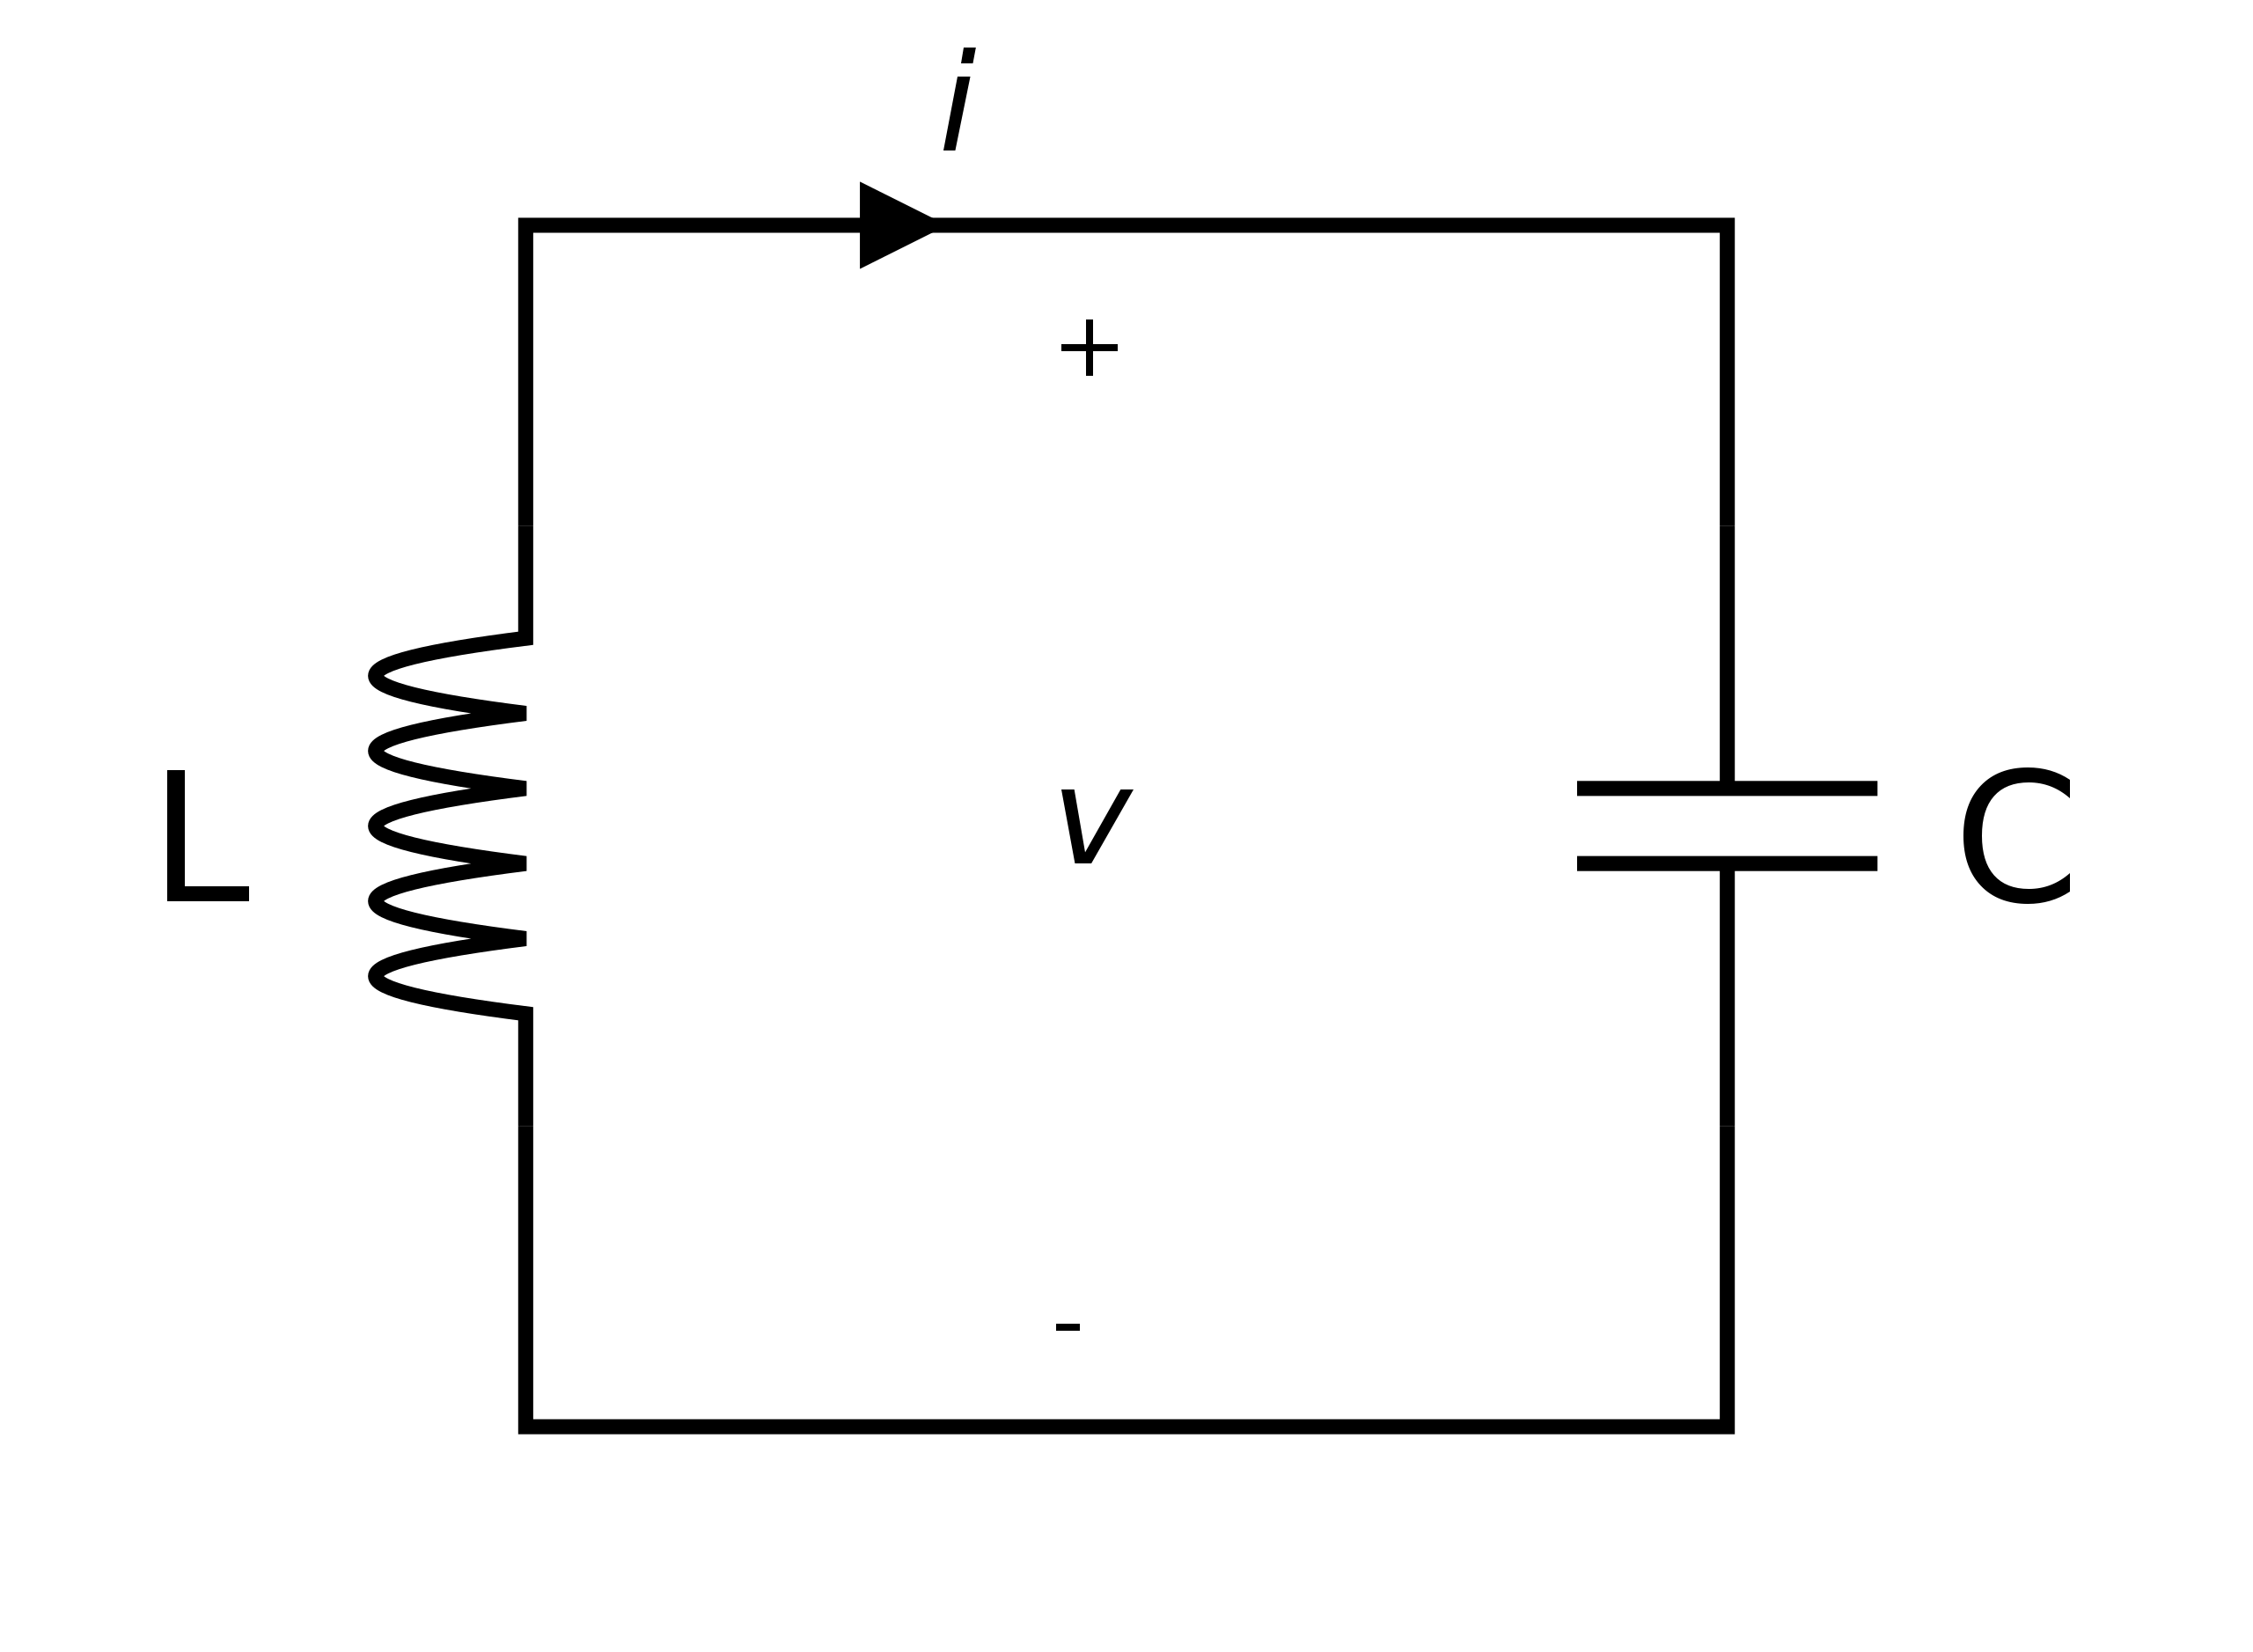
\includegraphics[width=0.6\textwidth]{images/2560px-LC_parallel_simple.svg.png}
    \caption{Schematics of a LC circuit}
    \label{fig:my_label}
\end{figure}

\subsection{Bandstop filter}




\section{Experimental arrangement}
schema

\section{Analysis}

\section{Conclusion}

\begin{appendix}
  \section{Additional Plots}
  \begin{figure}[H]
    \centering
    %% Creator: Matplotlib, PGF backend
%%
%% To include the figure in your LaTeX document, write
%%   \input{<filename>.pgf}
%%
%% Make sure the required packages are loaded in your preamble
%%   \usepackage{pgf}
%%
%% Also ensure that all the required font packages are loaded; for instance,
%% the lmodern package is sometimes necessary when using math font.
%%   \usepackage{lmodern}
%%
%% Figures using additional raster images can only be included by \input if
%% they are in the same directory as the main LaTeX file. For loading figures
%% from other directories you can use the `import` package
%%   \usepackage{import}
%%
%% and then include the figures with
%%   \import{<path to file>}{<filename>.pgf}
%%
%% Matplotlib used the following preamble
%%   
%%   \usepackage{fontspec}
%%   \setmainfont{DejaVuSerif.ttf}[Path=\detokenize{/usr/lib/python3.10/site-packages/matplotlib/mpl-data/fonts/ttf/}]
%%   \setsansfont{DejaVuSans.ttf}[Path=\detokenize{/usr/lib/python3.10/site-packages/matplotlib/mpl-data/fonts/ttf/}]
%%   \setmonofont{DejaVuSansMono.ttf}[Path=\detokenize{/usr/lib/python3.10/site-packages/matplotlib/mpl-data/fonts/ttf/}]
%%   \makeatletter\@ifpackageloaded{underscore}{}{\usepackage[strings]{underscore}}\makeatother
%%
\begingroup%
\makeatletter%
\begin{pgfpicture}%
\pgfpathrectangle{\pgfpointorigin}{\pgfqpoint{6.400000in}{4.800000in}}%
\pgfusepath{use as bounding box, clip}%
\begin{pgfscope}%
\pgfsetbuttcap%
\pgfsetmiterjoin%
\definecolor{currentfill}{rgb}{1.000000,1.000000,1.000000}%
\pgfsetfillcolor{currentfill}%
\pgfsetlinewidth{0.000000pt}%
\definecolor{currentstroke}{rgb}{1.000000,1.000000,1.000000}%
\pgfsetstrokecolor{currentstroke}%
\pgfsetdash{}{0pt}%
\pgfpathmoveto{\pgfqpoint{0.000000in}{0.000000in}}%
\pgfpathlineto{\pgfqpoint{6.400000in}{0.000000in}}%
\pgfpathlineto{\pgfqpoint{6.400000in}{4.800000in}}%
\pgfpathlineto{\pgfqpoint{0.000000in}{4.800000in}}%
\pgfpathlineto{\pgfqpoint{0.000000in}{0.000000in}}%
\pgfpathclose%
\pgfusepath{fill}%
\end{pgfscope}%
\begin{pgfscope}%
\pgfsetbuttcap%
\pgfsetmiterjoin%
\definecolor{currentfill}{rgb}{1.000000,1.000000,1.000000}%
\pgfsetfillcolor{currentfill}%
\pgfsetlinewidth{0.000000pt}%
\definecolor{currentstroke}{rgb}{0.000000,0.000000,0.000000}%
\pgfsetstrokecolor{currentstroke}%
\pgfsetstrokeopacity{0.000000}%
\pgfsetdash{}{0pt}%
\pgfpathmoveto{\pgfqpoint{0.800000in}{0.528000in}}%
\pgfpathlineto{\pgfqpoint{5.760000in}{0.528000in}}%
\pgfpathlineto{\pgfqpoint{5.760000in}{4.224000in}}%
\pgfpathlineto{\pgfqpoint{0.800000in}{4.224000in}}%
\pgfpathlineto{\pgfqpoint{0.800000in}{0.528000in}}%
\pgfpathclose%
\pgfusepath{fill}%
\end{pgfscope}%
\begin{pgfscope}%
\pgfsetbuttcap%
\pgfsetroundjoin%
\definecolor{currentfill}{rgb}{0.000000,0.000000,0.000000}%
\pgfsetfillcolor{currentfill}%
\pgfsetlinewidth{0.803000pt}%
\definecolor{currentstroke}{rgb}{0.000000,0.000000,0.000000}%
\pgfsetstrokecolor{currentstroke}%
\pgfsetdash{}{0pt}%
\pgfsys@defobject{currentmarker}{\pgfqpoint{0.000000in}{-0.048611in}}{\pgfqpoint{0.000000in}{0.000000in}}{%
\pgfpathmoveto{\pgfqpoint{0.000000in}{0.000000in}}%
\pgfpathlineto{\pgfqpoint{0.000000in}{-0.048611in}}%
\pgfusepath{stroke,fill}%
}%
\begin{pgfscope}%
\pgfsys@transformshift{1.025455in}{0.528000in}%
\pgfsys@useobject{currentmarker}{}%
\end{pgfscope}%
\end{pgfscope}%
\begin{pgfscope}%
\definecolor{textcolor}{rgb}{0.000000,0.000000,0.000000}%
\pgfsetstrokecolor{textcolor}%
\pgfsetfillcolor{textcolor}%
\pgftext[x=1.025455in,y=0.430778in,,top]{\color{textcolor}\sffamily\fontsize{10.000000}{12.000000}\selectfont \ensuremath{-}2.0}%
\end{pgfscope}%
\begin{pgfscope}%
\pgfsetbuttcap%
\pgfsetroundjoin%
\definecolor{currentfill}{rgb}{0.000000,0.000000,0.000000}%
\pgfsetfillcolor{currentfill}%
\pgfsetlinewidth{0.803000pt}%
\definecolor{currentstroke}{rgb}{0.000000,0.000000,0.000000}%
\pgfsetstrokecolor{currentstroke}%
\pgfsetdash{}{0pt}%
\pgfsys@defobject{currentmarker}{\pgfqpoint{0.000000in}{-0.048611in}}{\pgfqpoint{0.000000in}{0.000000in}}{%
\pgfpathmoveto{\pgfqpoint{0.000000in}{0.000000in}}%
\pgfpathlineto{\pgfqpoint{0.000000in}{-0.048611in}}%
\pgfusepath{stroke,fill}%
}%
\begin{pgfscope}%
\pgfsys@transformshift{1.589973in}{0.528000in}%
\pgfsys@useobject{currentmarker}{}%
\end{pgfscope}%
\end{pgfscope}%
\begin{pgfscope}%
\definecolor{textcolor}{rgb}{0.000000,0.000000,0.000000}%
\pgfsetstrokecolor{textcolor}%
\pgfsetfillcolor{textcolor}%
\pgftext[x=1.589973in,y=0.430778in,,top]{\color{textcolor}\sffamily\fontsize{10.000000}{12.000000}\selectfont \ensuremath{-}1.5}%
\end{pgfscope}%
\begin{pgfscope}%
\pgfsetbuttcap%
\pgfsetroundjoin%
\definecolor{currentfill}{rgb}{0.000000,0.000000,0.000000}%
\pgfsetfillcolor{currentfill}%
\pgfsetlinewidth{0.803000pt}%
\definecolor{currentstroke}{rgb}{0.000000,0.000000,0.000000}%
\pgfsetstrokecolor{currentstroke}%
\pgfsetdash{}{0pt}%
\pgfsys@defobject{currentmarker}{\pgfqpoint{0.000000in}{-0.048611in}}{\pgfqpoint{0.000000in}{0.000000in}}{%
\pgfpathmoveto{\pgfqpoint{0.000000in}{0.000000in}}%
\pgfpathlineto{\pgfqpoint{0.000000in}{-0.048611in}}%
\pgfusepath{stroke,fill}%
}%
\begin{pgfscope}%
\pgfsys@transformshift{2.154491in}{0.528000in}%
\pgfsys@useobject{currentmarker}{}%
\end{pgfscope}%
\end{pgfscope}%
\begin{pgfscope}%
\definecolor{textcolor}{rgb}{0.000000,0.000000,0.000000}%
\pgfsetstrokecolor{textcolor}%
\pgfsetfillcolor{textcolor}%
\pgftext[x=2.154491in,y=0.430778in,,top]{\color{textcolor}\sffamily\fontsize{10.000000}{12.000000}\selectfont \ensuremath{-}1.0}%
\end{pgfscope}%
\begin{pgfscope}%
\pgfsetbuttcap%
\pgfsetroundjoin%
\definecolor{currentfill}{rgb}{0.000000,0.000000,0.000000}%
\pgfsetfillcolor{currentfill}%
\pgfsetlinewidth{0.803000pt}%
\definecolor{currentstroke}{rgb}{0.000000,0.000000,0.000000}%
\pgfsetstrokecolor{currentstroke}%
\pgfsetdash{}{0pt}%
\pgfsys@defobject{currentmarker}{\pgfqpoint{0.000000in}{-0.048611in}}{\pgfqpoint{0.000000in}{0.000000in}}{%
\pgfpathmoveto{\pgfqpoint{0.000000in}{0.000000in}}%
\pgfpathlineto{\pgfqpoint{0.000000in}{-0.048611in}}%
\pgfusepath{stroke,fill}%
}%
\begin{pgfscope}%
\pgfsys@transformshift{2.719010in}{0.528000in}%
\pgfsys@useobject{currentmarker}{}%
\end{pgfscope}%
\end{pgfscope}%
\begin{pgfscope}%
\definecolor{textcolor}{rgb}{0.000000,0.000000,0.000000}%
\pgfsetstrokecolor{textcolor}%
\pgfsetfillcolor{textcolor}%
\pgftext[x=2.719010in,y=0.430778in,,top]{\color{textcolor}\sffamily\fontsize{10.000000}{12.000000}\selectfont \ensuremath{-}0.5}%
\end{pgfscope}%
\begin{pgfscope}%
\pgfsetbuttcap%
\pgfsetroundjoin%
\definecolor{currentfill}{rgb}{0.000000,0.000000,0.000000}%
\pgfsetfillcolor{currentfill}%
\pgfsetlinewidth{0.803000pt}%
\definecolor{currentstroke}{rgb}{0.000000,0.000000,0.000000}%
\pgfsetstrokecolor{currentstroke}%
\pgfsetdash{}{0pt}%
\pgfsys@defobject{currentmarker}{\pgfqpoint{0.000000in}{-0.048611in}}{\pgfqpoint{0.000000in}{0.000000in}}{%
\pgfpathmoveto{\pgfqpoint{0.000000in}{0.000000in}}%
\pgfpathlineto{\pgfqpoint{0.000000in}{-0.048611in}}%
\pgfusepath{stroke,fill}%
}%
\begin{pgfscope}%
\pgfsys@transformshift{3.283528in}{0.528000in}%
\pgfsys@useobject{currentmarker}{}%
\end{pgfscope}%
\end{pgfscope}%
\begin{pgfscope}%
\definecolor{textcolor}{rgb}{0.000000,0.000000,0.000000}%
\pgfsetstrokecolor{textcolor}%
\pgfsetfillcolor{textcolor}%
\pgftext[x=3.283528in,y=0.430778in,,top]{\color{textcolor}\sffamily\fontsize{10.000000}{12.000000}\selectfont 0.0}%
\end{pgfscope}%
\begin{pgfscope}%
\pgfsetbuttcap%
\pgfsetroundjoin%
\definecolor{currentfill}{rgb}{0.000000,0.000000,0.000000}%
\pgfsetfillcolor{currentfill}%
\pgfsetlinewidth{0.803000pt}%
\definecolor{currentstroke}{rgb}{0.000000,0.000000,0.000000}%
\pgfsetstrokecolor{currentstroke}%
\pgfsetdash{}{0pt}%
\pgfsys@defobject{currentmarker}{\pgfqpoint{0.000000in}{-0.048611in}}{\pgfqpoint{0.000000in}{0.000000in}}{%
\pgfpathmoveto{\pgfqpoint{0.000000in}{0.000000in}}%
\pgfpathlineto{\pgfqpoint{0.000000in}{-0.048611in}}%
\pgfusepath{stroke,fill}%
}%
\begin{pgfscope}%
\pgfsys@transformshift{3.848047in}{0.528000in}%
\pgfsys@useobject{currentmarker}{}%
\end{pgfscope}%
\end{pgfscope}%
\begin{pgfscope}%
\definecolor{textcolor}{rgb}{0.000000,0.000000,0.000000}%
\pgfsetstrokecolor{textcolor}%
\pgfsetfillcolor{textcolor}%
\pgftext[x=3.848047in,y=0.430778in,,top]{\color{textcolor}\sffamily\fontsize{10.000000}{12.000000}\selectfont 0.5}%
\end{pgfscope}%
\begin{pgfscope}%
\pgfsetbuttcap%
\pgfsetroundjoin%
\definecolor{currentfill}{rgb}{0.000000,0.000000,0.000000}%
\pgfsetfillcolor{currentfill}%
\pgfsetlinewidth{0.803000pt}%
\definecolor{currentstroke}{rgb}{0.000000,0.000000,0.000000}%
\pgfsetstrokecolor{currentstroke}%
\pgfsetdash{}{0pt}%
\pgfsys@defobject{currentmarker}{\pgfqpoint{0.000000in}{-0.048611in}}{\pgfqpoint{0.000000in}{0.000000in}}{%
\pgfpathmoveto{\pgfqpoint{0.000000in}{0.000000in}}%
\pgfpathlineto{\pgfqpoint{0.000000in}{-0.048611in}}%
\pgfusepath{stroke,fill}%
}%
\begin{pgfscope}%
\pgfsys@transformshift{4.412565in}{0.528000in}%
\pgfsys@useobject{currentmarker}{}%
\end{pgfscope}%
\end{pgfscope}%
\begin{pgfscope}%
\definecolor{textcolor}{rgb}{0.000000,0.000000,0.000000}%
\pgfsetstrokecolor{textcolor}%
\pgfsetfillcolor{textcolor}%
\pgftext[x=4.412565in,y=0.430778in,,top]{\color{textcolor}\sffamily\fontsize{10.000000}{12.000000}\selectfont 1.0}%
\end{pgfscope}%
\begin{pgfscope}%
\pgfsetbuttcap%
\pgfsetroundjoin%
\definecolor{currentfill}{rgb}{0.000000,0.000000,0.000000}%
\pgfsetfillcolor{currentfill}%
\pgfsetlinewidth{0.803000pt}%
\definecolor{currentstroke}{rgb}{0.000000,0.000000,0.000000}%
\pgfsetstrokecolor{currentstroke}%
\pgfsetdash{}{0pt}%
\pgfsys@defobject{currentmarker}{\pgfqpoint{0.000000in}{-0.048611in}}{\pgfqpoint{0.000000in}{0.000000in}}{%
\pgfpathmoveto{\pgfqpoint{0.000000in}{0.000000in}}%
\pgfpathlineto{\pgfqpoint{0.000000in}{-0.048611in}}%
\pgfusepath{stroke,fill}%
}%
\begin{pgfscope}%
\pgfsys@transformshift{4.977084in}{0.528000in}%
\pgfsys@useobject{currentmarker}{}%
\end{pgfscope}%
\end{pgfscope}%
\begin{pgfscope}%
\definecolor{textcolor}{rgb}{0.000000,0.000000,0.000000}%
\pgfsetstrokecolor{textcolor}%
\pgfsetfillcolor{textcolor}%
\pgftext[x=4.977084in,y=0.430778in,,top]{\color{textcolor}\sffamily\fontsize{10.000000}{12.000000}\selectfont 1.5}%
\end{pgfscope}%
\begin{pgfscope}%
\pgfsetbuttcap%
\pgfsetroundjoin%
\definecolor{currentfill}{rgb}{0.000000,0.000000,0.000000}%
\pgfsetfillcolor{currentfill}%
\pgfsetlinewidth{0.803000pt}%
\definecolor{currentstroke}{rgb}{0.000000,0.000000,0.000000}%
\pgfsetstrokecolor{currentstroke}%
\pgfsetdash{}{0pt}%
\pgfsys@defobject{currentmarker}{\pgfqpoint{0.000000in}{-0.048611in}}{\pgfqpoint{0.000000in}{0.000000in}}{%
\pgfpathmoveto{\pgfqpoint{0.000000in}{0.000000in}}%
\pgfpathlineto{\pgfqpoint{0.000000in}{-0.048611in}}%
\pgfusepath{stroke,fill}%
}%
\begin{pgfscope}%
\pgfsys@transformshift{5.541602in}{0.528000in}%
\pgfsys@useobject{currentmarker}{}%
\end{pgfscope}%
\end{pgfscope}%
\begin{pgfscope}%
\definecolor{textcolor}{rgb}{0.000000,0.000000,0.000000}%
\pgfsetstrokecolor{textcolor}%
\pgfsetfillcolor{textcolor}%
\pgftext[x=5.541602in,y=0.430778in,,top]{\color{textcolor}\sffamily\fontsize{10.000000}{12.000000}\selectfont 2.0}%
\end{pgfscope}%
\begin{pgfscope}%
\definecolor{textcolor}{rgb}{0.000000,0.000000,0.000000}%
\pgfsetstrokecolor{textcolor}%
\pgfsetfillcolor{textcolor}%
\pgftext[x=3.280000in,y=0.240809in,,top]{\color{textcolor}\sffamily\fontsize{10.000000}{12.000000}\selectfont Time / s}%
\end{pgfscope}%
\begin{pgfscope}%
\definecolor{textcolor}{rgb}{0.000000,0.000000,0.000000}%
\pgfsetstrokecolor{textcolor}%
\pgfsetfillcolor{textcolor}%
\pgftext[x=5.760000in,y=0.254698in,right,top]{\color{textcolor}\sffamily\fontsize{10.000000}{12.000000}\selectfont 1e\ensuremath{-}7}%
\end{pgfscope}%
\begin{pgfscope}%
\pgfsetbuttcap%
\pgfsetroundjoin%
\definecolor{currentfill}{rgb}{0.000000,0.000000,0.000000}%
\pgfsetfillcolor{currentfill}%
\pgfsetlinewidth{0.803000pt}%
\definecolor{currentstroke}{rgb}{0.000000,0.000000,0.000000}%
\pgfsetstrokecolor{currentstroke}%
\pgfsetdash{}{0pt}%
\pgfsys@defobject{currentmarker}{\pgfqpoint{-0.048611in}{0.000000in}}{\pgfqpoint{-0.000000in}{0.000000in}}{%
\pgfpathmoveto{\pgfqpoint{-0.000000in}{0.000000in}}%
\pgfpathlineto{\pgfqpoint{-0.048611in}{0.000000in}}%
\pgfusepath{stroke,fill}%
}%
\begin{pgfscope}%
\pgfsys@transformshift{0.800000in}{0.693759in}%
\pgfsys@useobject{currentmarker}{}%
\end{pgfscope}%
\end{pgfscope}%
\begin{pgfscope}%
\definecolor{textcolor}{rgb}{0.000000,0.000000,0.000000}%
\pgfsetstrokecolor{textcolor}%
\pgfsetfillcolor{textcolor}%
\pgftext[x=0.506387in, y=0.640998in, left, base]{\color{textcolor}\sffamily\fontsize{10.000000}{12.000000}\selectfont \ensuremath{-}4}%
\end{pgfscope}%
\begin{pgfscope}%
\pgfsetbuttcap%
\pgfsetroundjoin%
\definecolor{currentfill}{rgb}{0.000000,0.000000,0.000000}%
\pgfsetfillcolor{currentfill}%
\pgfsetlinewidth{0.803000pt}%
\definecolor{currentstroke}{rgb}{0.000000,0.000000,0.000000}%
\pgfsetstrokecolor{currentstroke}%
\pgfsetdash{}{0pt}%
\pgfsys@defobject{currentmarker}{\pgfqpoint{-0.048611in}{0.000000in}}{\pgfqpoint{-0.000000in}{0.000000in}}{%
\pgfpathmoveto{\pgfqpoint{-0.000000in}{0.000000in}}%
\pgfpathlineto{\pgfqpoint{-0.048611in}{0.000000in}}%
\pgfusepath{stroke,fill}%
}%
\begin{pgfscope}%
\pgfsys@transformshift{0.800000in}{1.164367in}%
\pgfsys@useobject{currentmarker}{}%
\end{pgfscope}%
\end{pgfscope}%
\begin{pgfscope}%
\definecolor{textcolor}{rgb}{0.000000,0.000000,0.000000}%
\pgfsetstrokecolor{textcolor}%
\pgfsetfillcolor{textcolor}%
\pgftext[x=0.506387in, y=1.111606in, left, base]{\color{textcolor}\sffamily\fontsize{10.000000}{12.000000}\selectfont \ensuremath{-}3}%
\end{pgfscope}%
\begin{pgfscope}%
\pgfsetbuttcap%
\pgfsetroundjoin%
\definecolor{currentfill}{rgb}{0.000000,0.000000,0.000000}%
\pgfsetfillcolor{currentfill}%
\pgfsetlinewidth{0.803000pt}%
\definecolor{currentstroke}{rgb}{0.000000,0.000000,0.000000}%
\pgfsetstrokecolor{currentstroke}%
\pgfsetdash{}{0pt}%
\pgfsys@defobject{currentmarker}{\pgfqpoint{-0.048611in}{0.000000in}}{\pgfqpoint{-0.000000in}{0.000000in}}{%
\pgfpathmoveto{\pgfqpoint{-0.000000in}{0.000000in}}%
\pgfpathlineto{\pgfqpoint{-0.048611in}{0.000000in}}%
\pgfusepath{stroke,fill}%
}%
\begin{pgfscope}%
\pgfsys@transformshift{0.800000in}{1.634975in}%
\pgfsys@useobject{currentmarker}{}%
\end{pgfscope}%
\end{pgfscope}%
\begin{pgfscope}%
\definecolor{textcolor}{rgb}{0.000000,0.000000,0.000000}%
\pgfsetstrokecolor{textcolor}%
\pgfsetfillcolor{textcolor}%
\pgftext[x=0.506387in, y=1.582214in, left, base]{\color{textcolor}\sffamily\fontsize{10.000000}{12.000000}\selectfont \ensuremath{-}2}%
\end{pgfscope}%
\begin{pgfscope}%
\pgfsetbuttcap%
\pgfsetroundjoin%
\definecolor{currentfill}{rgb}{0.000000,0.000000,0.000000}%
\pgfsetfillcolor{currentfill}%
\pgfsetlinewidth{0.803000pt}%
\definecolor{currentstroke}{rgb}{0.000000,0.000000,0.000000}%
\pgfsetstrokecolor{currentstroke}%
\pgfsetdash{}{0pt}%
\pgfsys@defobject{currentmarker}{\pgfqpoint{-0.048611in}{0.000000in}}{\pgfqpoint{-0.000000in}{0.000000in}}{%
\pgfpathmoveto{\pgfqpoint{-0.000000in}{0.000000in}}%
\pgfpathlineto{\pgfqpoint{-0.048611in}{0.000000in}}%
\pgfusepath{stroke,fill}%
}%
\begin{pgfscope}%
\pgfsys@transformshift{0.800000in}{2.105584in}%
\pgfsys@useobject{currentmarker}{}%
\end{pgfscope}%
\end{pgfscope}%
\begin{pgfscope}%
\definecolor{textcolor}{rgb}{0.000000,0.000000,0.000000}%
\pgfsetstrokecolor{textcolor}%
\pgfsetfillcolor{textcolor}%
\pgftext[x=0.506387in, y=2.052822in, left, base]{\color{textcolor}\sffamily\fontsize{10.000000}{12.000000}\selectfont \ensuremath{-}1}%
\end{pgfscope}%
\begin{pgfscope}%
\pgfsetbuttcap%
\pgfsetroundjoin%
\definecolor{currentfill}{rgb}{0.000000,0.000000,0.000000}%
\pgfsetfillcolor{currentfill}%
\pgfsetlinewidth{0.803000pt}%
\definecolor{currentstroke}{rgb}{0.000000,0.000000,0.000000}%
\pgfsetstrokecolor{currentstroke}%
\pgfsetdash{}{0pt}%
\pgfsys@defobject{currentmarker}{\pgfqpoint{-0.048611in}{0.000000in}}{\pgfqpoint{-0.000000in}{0.000000in}}{%
\pgfpathmoveto{\pgfqpoint{-0.000000in}{0.000000in}}%
\pgfpathlineto{\pgfqpoint{-0.048611in}{0.000000in}}%
\pgfusepath{stroke,fill}%
}%
\begin{pgfscope}%
\pgfsys@transformshift{0.800000in}{2.576192in}%
\pgfsys@useobject{currentmarker}{}%
\end{pgfscope}%
\end{pgfscope}%
\begin{pgfscope}%
\definecolor{textcolor}{rgb}{0.000000,0.000000,0.000000}%
\pgfsetstrokecolor{textcolor}%
\pgfsetfillcolor{textcolor}%
\pgftext[x=0.614412in, y=2.523430in, left, base]{\color{textcolor}\sffamily\fontsize{10.000000}{12.000000}\selectfont 0}%
\end{pgfscope}%
\begin{pgfscope}%
\pgfsetbuttcap%
\pgfsetroundjoin%
\definecolor{currentfill}{rgb}{0.000000,0.000000,0.000000}%
\pgfsetfillcolor{currentfill}%
\pgfsetlinewidth{0.803000pt}%
\definecolor{currentstroke}{rgb}{0.000000,0.000000,0.000000}%
\pgfsetstrokecolor{currentstroke}%
\pgfsetdash{}{0pt}%
\pgfsys@defobject{currentmarker}{\pgfqpoint{-0.048611in}{0.000000in}}{\pgfqpoint{-0.000000in}{0.000000in}}{%
\pgfpathmoveto{\pgfqpoint{-0.000000in}{0.000000in}}%
\pgfpathlineto{\pgfqpoint{-0.048611in}{0.000000in}}%
\pgfusepath{stroke,fill}%
}%
\begin{pgfscope}%
\pgfsys@transformshift{0.800000in}{3.046800in}%
\pgfsys@useobject{currentmarker}{}%
\end{pgfscope}%
\end{pgfscope}%
\begin{pgfscope}%
\definecolor{textcolor}{rgb}{0.000000,0.000000,0.000000}%
\pgfsetstrokecolor{textcolor}%
\pgfsetfillcolor{textcolor}%
\pgftext[x=0.614412in, y=2.994038in, left, base]{\color{textcolor}\sffamily\fontsize{10.000000}{12.000000}\selectfont 1}%
\end{pgfscope}%
\begin{pgfscope}%
\pgfsetbuttcap%
\pgfsetroundjoin%
\definecolor{currentfill}{rgb}{0.000000,0.000000,0.000000}%
\pgfsetfillcolor{currentfill}%
\pgfsetlinewidth{0.803000pt}%
\definecolor{currentstroke}{rgb}{0.000000,0.000000,0.000000}%
\pgfsetstrokecolor{currentstroke}%
\pgfsetdash{}{0pt}%
\pgfsys@defobject{currentmarker}{\pgfqpoint{-0.048611in}{0.000000in}}{\pgfqpoint{-0.000000in}{0.000000in}}{%
\pgfpathmoveto{\pgfqpoint{-0.000000in}{0.000000in}}%
\pgfpathlineto{\pgfqpoint{-0.048611in}{0.000000in}}%
\pgfusepath{stroke,fill}%
}%
\begin{pgfscope}%
\pgfsys@transformshift{0.800000in}{3.517408in}%
\pgfsys@useobject{currentmarker}{}%
\end{pgfscope}%
\end{pgfscope}%
\begin{pgfscope}%
\definecolor{textcolor}{rgb}{0.000000,0.000000,0.000000}%
\pgfsetstrokecolor{textcolor}%
\pgfsetfillcolor{textcolor}%
\pgftext[x=0.614412in, y=3.464646in, left, base]{\color{textcolor}\sffamily\fontsize{10.000000}{12.000000}\selectfont 2}%
\end{pgfscope}%
\begin{pgfscope}%
\pgfsetbuttcap%
\pgfsetroundjoin%
\definecolor{currentfill}{rgb}{0.000000,0.000000,0.000000}%
\pgfsetfillcolor{currentfill}%
\pgfsetlinewidth{0.803000pt}%
\definecolor{currentstroke}{rgb}{0.000000,0.000000,0.000000}%
\pgfsetstrokecolor{currentstroke}%
\pgfsetdash{}{0pt}%
\pgfsys@defobject{currentmarker}{\pgfqpoint{-0.048611in}{0.000000in}}{\pgfqpoint{-0.000000in}{0.000000in}}{%
\pgfpathmoveto{\pgfqpoint{-0.000000in}{0.000000in}}%
\pgfpathlineto{\pgfqpoint{-0.048611in}{0.000000in}}%
\pgfusepath{stroke,fill}%
}%
\begin{pgfscope}%
\pgfsys@transformshift{0.800000in}{3.988016in}%
\pgfsys@useobject{currentmarker}{}%
\end{pgfscope}%
\end{pgfscope}%
\begin{pgfscope}%
\definecolor{textcolor}{rgb}{0.000000,0.000000,0.000000}%
\pgfsetstrokecolor{textcolor}%
\pgfsetfillcolor{textcolor}%
\pgftext[x=0.614412in, y=3.935255in, left, base]{\color{textcolor}\sffamily\fontsize{10.000000}{12.000000}\selectfont 3}%
\end{pgfscope}%
\begin{pgfscope}%
\definecolor{textcolor}{rgb}{0.000000,0.000000,0.000000}%
\pgfsetstrokecolor{textcolor}%
\pgfsetfillcolor{textcolor}%
\pgftext[x=0.450832in,y=2.376000in,,bottom,rotate=90.000000]{\color{textcolor}\sffamily\fontsize{10.000000}{12.000000}\selectfont Voltage / V}%
\end{pgfscope}%
\begin{pgfscope}%
\pgfpathrectangle{\pgfqpoint{0.800000in}{0.528000in}}{\pgfqpoint{4.960000in}{3.696000in}}%
\pgfusepath{clip}%
\pgfsetrectcap%
\pgfsetroundjoin%
\pgfsetlinewidth{1.505625pt}%
\definecolor{currentstroke}{rgb}{0.121569,0.466667,0.705882}%
\pgfsetstrokecolor{currentstroke}%
\pgfsetdash{}{0pt}%
\pgfpathmoveto{\pgfqpoint{1.025455in}{0.883259in}}%
\pgfpathlineto{\pgfqpoint{1.103076in}{0.883259in}}%
\pgfpathlineto{\pgfqpoint{1.110132in}{0.845421in}}%
\pgfpathlineto{\pgfqpoint{1.166584in}{0.845421in}}%
\pgfpathlineto{\pgfqpoint{1.180697in}{0.883259in}}%
\pgfpathlineto{\pgfqpoint{1.279488in}{0.883259in}}%
\pgfpathlineto{\pgfqpoint{1.293601in}{0.921096in}}%
\pgfpathlineto{\pgfqpoint{1.357109in}{0.921096in}}%
\pgfpathlineto{\pgfqpoint{1.364166in}{0.904542in}}%
\pgfpathlineto{\pgfqpoint{1.371222in}{0.883259in}}%
\pgfpathlineto{\pgfqpoint{1.392392in}{0.883259in}}%
\pgfpathlineto{\pgfqpoint{1.406504in}{0.921096in}}%
\pgfpathlineto{\pgfqpoint{1.413561in}{0.883259in}}%
\pgfpathlineto{\pgfqpoint{1.582916in}{0.883259in}}%
\pgfpathlineto{\pgfqpoint{1.589973in}{0.866705in}}%
\pgfpathlineto{\pgfqpoint{1.597029in}{0.845421in}}%
\pgfpathlineto{\pgfqpoint{1.604086in}{0.869069in}}%
\pgfpathlineto{\pgfqpoint{1.611142in}{0.883259in}}%
\pgfpathlineto{\pgfqpoint{1.695820in}{0.883259in}}%
\pgfpathlineto{\pgfqpoint{1.702877in}{0.866705in}}%
\pgfpathlineto{\pgfqpoint{1.709933in}{0.845421in}}%
\pgfpathlineto{\pgfqpoint{1.836950in}{0.845421in}}%
\pgfpathlineto{\pgfqpoint{1.844006in}{0.883259in}}%
\pgfpathlineto{\pgfqpoint{1.914571in}{0.883259in}}%
\pgfpathlineto{\pgfqpoint{1.921628in}{0.845421in}}%
\pgfpathlineto{\pgfqpoint{1.935741in}{0.845421in}}%
\pgfpathlineto{\pgfqpoint{1.942797in}{0.869069in}}%
\pgfpathlineto{\pgfqpoint{1.949853in}{0.883259in}}%
\pgfpathlineto{\pgfqpoint{2.083927in}{0.883259in}}%
\pgfpathlineto{\pgfqpoint{2.090983in}{0.921096in}}%
\pgfpathlineto{\pgfqpoint{2.140378in}{0.921096in}}%
\pgfpathlineto{\pgfqpoint{2.147435in}{0.883259in}}%
\pgfpathlineto{\pgfqpoint{2.218000in}{0.883259in}}%
\pgfpathlineto{\pgfqpoint{2.225056in}{0.857245in}}%
\pgfpathlineto{\pgfqpoint{2.232113in}{0.845421in}}%
\pgfpathlineto{\pgfqpoint{2.239169in}{0.883259in}}%
\pgfpathlineto{\pgfqpoint{2.330903in}{0.883259in}}%
\pgfpathlineto{\pgfqpoint{2.337960in}{0.906907in}}%
\pgfpathlineto{\pgfqpoint{2.345016in}{0.921096in}}%
\pgfpathlineto{\pgfqpoint{2.366186in}{0.921096in}}%
\pgfpathlineto{\pgfqpoint{2.373242in}{0.883259in}}%
\pgfpathlineto{\pgfqpoint{2.380299in}{0.897448in}}%
\pgfpathlineto{\pgfqpoint{2.387355in}{0.921096in}}%
\pgfpathlineto{\pgfqpoint{2.443807in}{0.921096in}}%
\pgfpathlineto{\pgfqpoint{2.450864in}{0.895083in}}%
\pgfpathlineto{\pgfqpoint{2.457920in}{0.883259in}}%
\pgfpathlineto{\pgfqpoint{2.577880in}{0.883259in}}%
\pgfpathlineto{\pgfqpoint{2.584937in}{0.861975in}}%
\pgfpathlineto{\pgfqpoint{2.591993in}{0.845421in}}%
\pgfpathlineto{\pgfqpoint{2.648445in}{0.845421in}}%
\pgfpathlineto{\pgfqpoint{2.655501in}{0.883259in}}%
\pgfpathlineto{\pgfqpoint{3.022438in}{0.883259in}}%
\pgfpathlineto{\pgfqpoint{3.029495in}{0.921096in}}%
\pgfpathlineto{\pgfqpoint{3.085947in}{0.921096in}}%
\pgfpathlineto{\pgfqpoint{3.100060in}{0.958934in}}%
\pgfpathlineto{\pgfqpoint{3.107116in}{0.958934in}}%
\pgfpathlineto{\pgfqpoint{3.114173in}{0.973124in}}%
\pgfpathlineto{\pgfqpoint{3.121229in}{0.996772in}}%
\pgfpathlineto{\pgfqpoint{3.135342in}{0.996772in}}%
\pgfpathlineto{\pgfqpoint{3.142399in}{1.072448in}}%
\pgfpathlineto{\pgfqpoint{3.156512in}{1.110286in}}%
\pgfpathlineto{\pgfqpoint{3.163568in}{1.148124in}}%
\pgfpathlineto{\pgfqpoint{3.170625in}{1.176502in}}%
\pgfpathlineto{\pgfqpoint{3.177681in}{1.223799in}}%
\pgfpathlineto{\pgfqpoint{3.184738in}{1.247448in}}%
\pgfpathlineto{\pgfqpoint{3.191794in}{1.261637in}}%
\pgfpathlineto{\pgfqpoint{3.198850in}{1.337313in}}%
\pgfpathlineto{\pgfqpoint{3.212963in}{1.375151in}}%
\pgfpathlineto{\pgfqpoint{3.220020in}{1.450826in}}%
\pgfpathlineto{\pgfqpoint{3.227076in}{1.479205in}}%
\pgfpathlineto{\pgfqpoint{3.241189in}{1.573799in}}%
\pgfpathlineto{\pgfqpoint{3.248246in}{1.602178in}}%
\pgfpathlineto{\pgfqpoint{3.269415in}{1.715691in}}%
\pgfpathlineto{\pgfqpoint{3.276472in}{1.791367in}}%
\pgfpathlineto{\pgfqpoint{3.283528in}{1.805556in}}%
\pgfpathlineto{\pgfqpoint{3.290585in}{1.829205in}}%
\pgfpathlineto{\pgfqpoint{3.297641in}{1.876502in}}%
\pgfpathlineto{\pgfqpoint{3.304698in}{1.904880in}}%
\pgfpathlineto{\pgfqpoint{3.332924in}{2.056232in}}%
\pgfpathlineto{\pgfqpoint{3.339980in}{2.084610in}}%
\pgfpathlineto{\pgfqpoint{3.347037in}{2.131907in}}%
\pgfpathlineto{\pgfqpoint{3.354093in}{2.155556in}}%
\pgfpathlineto{\pgfqpoint{3.361150in}{2.169745in}}%
\pgfpathlineto{\pgfqpoint{3.389375in}{2.321096in}}%
\pgfpathlineto{\pgfqpoint{3.403488in}{2.321096in}}%
\pgfpathlineto{\pgfqpoint{3.410545in}{2.344745in}}%
\pgfpathlineto{\pgfqpoint{3.417601in}{2.358934in}}%
\pgfpathlineto{\pgfqpoint{3.424658in}{2.396772in}}%
\pgfpathlineto{\pgfqpoint{3.438771in}{2.434610in}}%
\pgfpathlineto{\pgfqpoint{3.445827in}{2.434610in}}%
\pgfpathlineto{\pgfqpoint{3.452884in}{2.448799in}}%
\pgfpathlineto{\pgfqpoint{3.459940in}{2.472448in}}%
\pgfpathlineto{\pgfqpoint{3.474053in}{2.472448in}}%
\pgfpathlineto{\pgfqpoint{3.481110in}{2.510286in}}%
\pgfpathlineto{\pgfqpoint{3.502279in}{2.510286in}}%
\pgfpathlineto{\pgfqpoint{3.509336in}{2.493732in}}%
\pgfpathlineto{\pgfqpoint{3.516392in}{2.472448in}}%
\pgfpathlineto{\pgfqpoint{3.530505in}{2.472448in}}%
\pgfpathlineto{\pgfqpoint{3.537562in}{2.434610in}}%
\pgfpathlineto{\pgfqpoint{3.544618in}{2.413326in}}%
\pgfpathlineto{\pgfqpoint{3.551674in}{2.396772in}}%
\pgfpathlineto{\pgfqpoint{3.558731in}{2.396772in}}%
\pgfpathlineto{\pgfqpoint{3.565787in}{2.380218in}}%
\pgfpathlineto{\pgfqpoint{3.572844in}{2.358934in}}%
\pgfpathlineto{\pgfqpoint{3.579900in}{2.332921in}}%
\pgfpathlineto{\pgfqpoint{3.586957in}{2.321096in}}%
\pgfpathlineto{\pgfqpoint{3.594013in}{2.283259in}}%
\pgfpathlineto{\pgfqpoint{3.601070in}{2.261975in}}%
\pgfpathlineto{\pgfqpoint{3.608126in}{2.245421in}}%
\pgfpathlineto{\pgfqpoint{3.615183in}{2.207583in}}%
\pgfpathlineto{\pgfqpoint{3.622239in}{2.191029in}}%
\pgfpathlineto{\pgfqpoint{3.629296in}{2.169745in}}%
\pgfpathlineto{\pgfqpoint{3.643409in}{2.169745in}}%
\pgfpathlineto{\pgfqpoint{3.650465in}{2.131907in}}%
\pgfpathlineto{\pgfqpoint{3.664578in}{2.131907in}}%
\pgfpathlineto{\pgfqpoint{3.671635in}{2.094069in}}%
\pgfpathlineto{\pgfqpoint{3.699861in}{2.094069in}}%
\pgfpathlineto{\pgfqpoint{3.706917in}{2.056232in}}%
\pgfpathlineto{\pgfqpoint{3.721030in}{2.056232in}}%
\pgfpathlineto{\pgfqpoint{3.728086in}{2.018394in}}%
\pgfpathlineto{\pgfqpoint{3.742199in}{2.018394in}}%
\pgfpathlineto{\pgfqpoint{3.749256in}{1.992380in}}%
\pgfpathlineto{\pgfqpoint{3.756312in}{1.980556in}}%
\pgfpathlineto{\pgfqpoint{3.763369in}{1.942718in}}%
\pgfpathlineto{\pgfqpoint{3.770425in}{1.921434in}}%
\pgfpathlineto{\pgfqpoint{3.777482in}{1.904880in}}%
\pgfpathlineto{\pgfqpoint{3.784538in}{1.867042in}}%
\pgfpathlineto{\pgfqpoint{3.791595in}{1.850488in}}%
\pgfpathlineto{\pgfqpoint{3.798651in}{1.829205in}}%
\pgfpathlineto{\pgfqpoint{3.805708in}{1.803191in}}%
\pgfpathlineto{\pgfqpoint{3.812764in}{1.791367in}}%
\pgfpathlineto{\pgfqpoint{3.819821in}{1.791367in}}%
\pgfpathlineto{\pgfqpoint{3.826877in}{1.770083in}}%
\pgfpathlineto{\pgfqpoint{3.833934in}{1.753529in}}%
\pgfpathlineto{\pgfqpoint{3.840990in}{1.715691in}}%
\pgfpathlineto{\pgfqpoint{3.848047in}{1.699137in}}%
\pgfpathlineto{\pgfqpoint{3.855103in}{1.677853in}}%
\pgfpathlineto{\pgfqpoint{3.862160in}{1.651840in}}%
\pgfpathlineto{\pgfqpoint{3.869216in}{1.640015in}}%
\pgfpathlineto{\pgfqpoint{3.876273in}{1.602178in}}%
\pgfpathlineto{\pgfqpoint{3.883329in}{1.580894in}}%
\pgfpathlineto{\pgfqpoint{3.890386in}{1.564340in}}%
\pgfpathlineto{\pgfqpoint{3.897442in}{1.564340in}}%
\pgfpathlineto{\pgfqpoint{3.904499in}{1.547786in}}%
\pgfpathlineto{\pgfqpoint{3.911555in}{1.526502in}}%
\pgfpathlineto{\pgfqpoint{3.925668in}{1.526502in}}%
\pgfpathlineto{\pgfqpoint{3.932724in}{1.488664in}}%
\pgfpathlineto{\pgfqpoint{3.968007in}{1.488664in}}%
\pgfpathlineto{\pgfqpoint{3.975063in}{1.462651in}}%
\pgfpathlineto{\pgfqpoint{3.982120in}{1.450826in}}%
\pgfpathlineto{\pgfqpoint{4.024459in}{1.450826in}}%
\pgfpathlineto{\pgfqpoint{4.031515in}{1.424813in}}%
\pgfpathlineto{\pgfqpoint{4.038572in}{1.412988in}}%
\pgfpathlineto{\pgfqpoint{4.045628in}{1.412988in}}%
\pgfpathlineto{\pgfqpoint{4.052685in}{1.391705in}}%
\pgfpathlineto{\pgfqpoint{4.059741in}{1.375151in}}%
\pgfpathlineto{\pgfqpoint{4.066798in}{1.375151in}}%
\pgfpathlineto{\pgfqpoint{4.073854in}{1.358596in}}%
\pgfpathlineto{\pgfqpoint{4.080911in}{1.337313in}}%
\pgfpathlineto{\pgfqpoint{4.095023in}{1.337313in}}%
\pgfpathlineto{\pgfqpoint{4.102080in}{1.299475in}}%
\pgfpathlineto{\pgfqpoint{4.116193in}{1.299475in}}%
\pgfpathlineto{\pgfqpoint{4.123249in}{1.261637in}}%
\pgfpathlineto{\pgfqpoint{4.229097in}{1.261637in}}%
\pgfpathlineto{\pgfqpoint{4.236153in}{1.223799in}}%
\pgfpathlineto{\pgfqpoint{4.271435in}{1.223799in}}%
\pgfpathlineto{\pgfqpoint{4.278492in}{1.202515in}}%
\pgfpathlineto{\pgfqpoint{4.285548in}{1.185961in}}%
\pgfpathlineto{\pgfqpoint{4.292605in}{1.185961in}}%
\pgfpathlineto{\pgfqpoint{4.299661in}{1.169407in}}%
\pgfpathlineto{\pgfqpoint{4.306718in}{1.148124in}}%
\pgfpathlineto{\pgfqpoint{4.320831in}{1.148124in}}%
\pgfpathlineto{\pgfqpoint{4.327887in}{1.110286in}}%
\pgfpathlineto{\pgfqpoint{4.440791in}{1.110286in}}%
\pgfpathlineto{\pgfqpoint{4.447847in}{1.089002in}}%
\pgfpathlineto{\pgfqpoint{4.454904in}{1.072448in}}%
\pgfpathlineto{\pgfqpoint{4.476073in}{1.072448in}}%
\pgfpathlineto{\pgfqpoint{4.483130in}{1.046434in}}%
\pgfpathlineto{\pgfqpoint{4.490186in}{1.034610in}}%
\pgfpathlineto{\pgfqpoint{4.518412in}{1.034610in}}%
\pgfpathlineto{\pgfqpoint{4.525469in}{1.018056in}}%
\pgfpathlineto{\pgfqpoint{4.532525in}{0.996772in}}%
\pgfpathlineto{\pgfqpoint{4.610147in}{0.996772in}}%
\pgfpathlineto{\pgfqpoint{4.624259in}{1.034610in}}%
\pgfpathlineto{\pgfqpoint{4.659542in}{1.034610in}}%
\pgfpathlineto{\pgfqpoint{4.666598in}{0.996772in}}%
\pgfpathlineto{\pgfqpoint{4.687768in}{0.996772in}}%
\pgfpathlineto{\pgfqpoint{4.694824in}{0.980218in}}%
\pgfpathlineto{\pgfqpoint{4.701881in}{0.958934in}}%
\pgfpathlineto{\pgfqpoint{4.737163in}{0.958934in}}%
\pgfpathlineto{\pgfqpoint{4.744220in}{0.921096in}}%
\pgfpathlineto{\pgfqpoint{4.772446in}{0.921096in}}%
\pgfpathlineto{\pgfqpoint{4.779502in}{0.883259in}}%
\pgfpathlineto{\pgfqpoint{4.793615in}{0.883259in}}%
\pgfpathlineto{\pgfqpoint{4.800672in}{0.921096in}}%
\pgfpathlineto{\pgfqpoint{4.828897in}{0.921096in}}%
\pgfpathlineto{\pgfqpoint{4.835954in}{0.958934in}}%
\pgfpathlineto{\pgfqpoint{4.857123in}{0.958934in}}%
\pgfpathlineto{\pgfqpoint{4.864180in}{0.973124in}}%
\pgfpathlineto{\pgfqpoint{4.871236in}{0.996772in}}%
\pgfpathlineto{\pgfqpoint{4.878293in}{0.970759in}}%
\pgfpathlineto{\pgfqpoint{4.885349in}{0.958934in}}%
\pgfpathlineto{\pgfqpoint{4.913575in}{0.958934in}}%
\pgfpathlineto{\pgfqpoint{4.920632in}{0.942380in}}%
\pgfpathlineto{\pgfqpoint{4.927688in}{0.921096in}}%
\pgfpathlineto{\pgfqpoint{4.970027in}{0.921096in}}%
\pgfpathlineto{\pgfqpoint{4.977084in}{0.904542in}}%
\pgfpathlineto{\pgfqpoint{4.984140in}{0.883259in}}%
\pgfpathlineto{\pgfqpoint{5.026479in}{0.883259in}}%
\pgfpathlineto{\pgfqpoint{5.033535in}{0.866705in}}%
\pgfpathlineto{\pgfqpoint{5.040592in}{0.845421in}}%
\pgfpathlineto{\pgfqpoint{5.075874in}{0.845421in}}%
\pgfpathlineto{\pgfqpoint{5.082931in}{0.883259in}}%
\pgfpathlineto{\pgfqpoint{5.132326in}{0.883259in}}%
\pgfpathlineto{\pgfqpoint{5.139383in}{0.921096in}}%
\pgfpathlineto{\pgfqpoint{5.344020in}{0.921096in}}%
\pgfpathlineto{\pgfqpoint{5.351077in}{0.899813in}}%
\pgfpathlineto{\pgfqpoint{5.358133in}{0.883259in}}%
\pgfpathlineto{\pgfqpoint{5.421642in}{0.883259in}}%
\pgfpathlineto{\pgfqpoint{5.428698in}{0.866705in}}%
\pgfpathlineto{\pgfqpoint{5.435755in}{0.845421in}}%
\pgfpathlineto{\pgfqpoint{5.449868in}{0.845421in}}%
\pgfpathlineto{\pgfqpoint{5.456924in}{0.883259in}}%
\pgfpathlineto{\pgfqpoint{5.534545in}{0.883259in}}%
\pgfpathlineto{\pgfqpoint{5.534545in}{0.883259in}}%
\pgfusepath{stroke}%
\end{pgfscope}%
\begin{pgfscope}%
\pgfpathrectangle{\pgfqpoint{0.800000in}{0.528000in}}{\pgfqpoint{4.960000in}{3.696000in}}%
\pgfusepath{clip}%
\pgfsetrectcap%
\pgfsetroundjoin%
\pgfsetlinewidth{1.505625pt}%
\definecolor{currentstroke}{rgb}{1.000000,0.498039,0.054902}%
\pgfsetstrokecolor{currentstroke}%
\pgfsetdash{}{0pt}%
\pgfpathmoveto{\pgfqpoint{1.025455in}{0.832216in}}%
\pgfpathlineto{\pgfqpoint{1.032511in}{0.860595in}}%
\pgfpathlineto{\pgfqpoint{1.039568in}{0.877622in}}%
\pgfpathlineto{\pgfqpoint{1.081906in}{0.877622in}}%
\pgfpathlineto{\pgfqpoint{1.088963in}{0.846405in}}%
\pgfpathlineto{\pgfqpoint{1.096019in}{0.832216in}}%
\pgfpathlineto{\pgfqpoint{1.103076in}{0.877622in}}%
\pgfpathlineto{\pgfqpoint{1.110132in}{0.852081in}}%
\pgfpathlineto{\pgfqpoint{1.117189in}{0.832216in}}%
\pgfpathlineto{\pgfqpoint{1.138358in}{0.832216in}}%
\pgfpathlineto{\pgfqpoint{1.145415in}{0.860595in}}%
\pgfpathlineto{\pgfqpoint{1.152471in}{0.877622in}}%
\pgfpathlineto{\pgfqpoint{1.272431in}{0.877622in}}%
\pgfpathlineto{\pgfqpoint{1.286544in}{0.923027in}}%
\pgfpathlineto{\pgfqpoint{1.293601in}{0.877622in}}%
\pgfpathlineto{\pgfqpoint{1.342996in}{0.877622in}}%
\pgfpathlineto{\pgfqpoint{1.350053in}{0.832216in}}%
\pgfpathlineto{\pgfqpoint{1.364166in}{0.832216in}}%
\pgfpathlineto{\pgfqpoint{1.371222in}{0.860595in}}%
\pgfpathlineto{\pgfqpoint{1.378279in}{0.877622in}}%
\pgfpathlineto{\pgfqpoint{1.406504in}{0.877622in}}%
\pgfpathlineto{\pgfqpoint{1.413561in}{0.894649in}}%
\pgfpathlineto{\pgfqpoint{1.420617in}{0.923027in}}%
\pgfpathlineto{\pgfqpoint{1.491182in}{0.923027in}}%
\pgfpathlineto{\pgfqpoint{1.498239in}{0.877622in}}%
\pgfpathlineto{\pgfqpoint{1.547634in}{0.877622in}}%
\pgfpathlineto{\pgfqpoint{1.554691in}{0.832216in}}%
\pgfpathlineto{\pgfqpoint{1.575860in}{0.832216in}}%
\pgfpathlineto{\pgfqpoint{1.582916in}{0.849243in}}%
\pgfpathlineto{\pgfqpoint{1.589973in}{0.877622in}}%
\pgfpathlineto{\pgfqpoint{1.738159in}{0.877622in}}%
\pgfpathlineto{\pgfqpoint{1.745216in}{0.832216in}}%
\pgfpathlineto{\pgfqpoint{1.836950in}{0.832216in}}%
\pgfpathlineto{\pgfqpoint{1.851063in}{0.877622in}}%
\pgfpathlineto{\pgfqpoint{1.872232in}{0.877622in}}%
\pgfpathlineto{\pgfqpoint{1.879289in}{0.906000in}}%
\pgfpathlineto{\pgfqpoint{1.886345in}{0.923027in}}%
\pgfpathlineto{\pgfqpoint{1.914571in}{0.923027in}}%
\pgfpathlineto{\pgfqpoint{1.921628in}{0.903162in}}%
\pgfpathlineto{\pgfqpoint{1.928684in}{0.877622in}}%
\pgfpathlineto{\pgfqpoint{1.971023in}{0.877622in}}%
\pgfpathlineto{\pgfqpoint{1.978079in}{0.857757in}}%
\pgfpathlineto{\pgfqpoint{1.985136in}{0.832216in}}%
\pgfpathlineto{\pgfqpoint{2.062757in}{0.832216in}}%
\pgfpathlineto{\pgfqpoint{2.076870in}{0.877622in}}%
\pgfpathlineto{\pgfqpoint{2.168604in}{0.877622in}}%
\pgfpathlineto{\pgfqpoint{2.175661in}{0.832216in}}%
\pgfpathlineto{\pgfqpoint{2.232113in}{0.832216in}}%
\pgfpathlineto{\pgfqpoint{2.246226in}{0.877622in}}%
\pgfpathlineto{\pgfqpoint{2.401468in}{0.877622in}}%
\pgfpathlineto{\pgfqpoint{2.415581in}{0.923027in}}%
\pgfpathlineto{\pgfqpoint{2.422638in}{0.923027in}}%
\pgfpathlineto{\pgfqpoint{2.429694in}{0.903162in}}%
\pgfpathlineto{\pgfqpoint{2.436751in}{0.877622in}}%
\pgfpathlineto{\pgfqpoint{2.507315in}{0.877622in}}%
\pgfpathlineto{\pgfqpoint{2.514372in}{0.832216in}}%
\pgfpathlineto{\pgfqpoint{2.606106in}{0.832216in}}%
\pgfpathlineto{\pgfqpoint{2.613163in}{0.860595in}}%
\pgfpathlineto{\pgfqpoint{2.620219in}{0.877622in}}%
\pgfpathlineto{\pgfqpoint{2.733123in}{0.877622in}}%
\pgfpathlineto{\pgfqpoint{2.740179in}{0.832216in}}%
\pgfpathlineto{\pgfqpoint{2.817801in}{0.832216in}}%
\pgfpathlineto{\pgfqpoint{2.824857in}{0.849243in}}%
\pgfpathlineto{\pgfqpoint{2.831914in}{0.877622in}}%
\pgfpathlineto{\pgfqpoint{2.838970in}{0.846405in}}%
\pgfpathlineto{\pgfqpoint{2.846026in}{0.832216in}}%
\pgfpathlineto{\pgfqpoint{2.888365in}{0.832216in}}%
\pgfpathlineto{\pgfqpoint{2.895422in}{0.860595in}}%
\pgfpathlineto{\pgfqpoint{2.902478in}{0.877622in}}%
\pgfpathlineto{\pgfqpoint{2.965987in}{0.877622in}}%
\pgfpathlineto{\pgfqpoint{2.973043in}{0.852081in}}%
\pgfpathlineto{\pgfqpoint{2.980100in}{0.832216in}}%
\pgfpathlineto{\pgfqpoint{2.987156in}{0.832216in}}%
\pgfpathlineto{\pgfqpoint{2.994213in}{0.849243in}}%
\pgfpathlineto{\pgfqpoint{3.001269in}{0.877622in}}%
\pgfpathlineto{\pgfqpoint{3.036551in}{0.877622in}}%
\pgfpathlineto{\pgfqpoint{3.043608in}{0.923027in}}%
\pgfpathlineto{\pgfqpoint{3.071834in}{0.923027in}}%
\pgfpathlineto{\pgfqpoint{3.078890in}{0.968432in}}%
\pgfpathlineto{\pgfqpoint{3.093003in}{0.968432in}}%
\pgfpathlineto{\pgfqpoint{3.100060in}{1.013838in}}%
\pgfpathlineto{\pgfqpoint{3.107116in}{1.030865in}}%
\pgfpathlineto{\pgfqpoint{3.121229in}{1.087622in}}%
\pgfpathlineto{\pgfqpoint{3.128286in}{1.104649in}}%
\pgfpathlineto{\pgfqpoint{3.135342in}{1.150054in}}%
\pgfpathlineto{\pgfqpoint{3.149455in}{1.195459in}}%
\pgfpathlineto{\pgfqpoint{3.156512in}{1.286270in}}%
\pgfpathlineto{\pgfqpoint{3.163568in}{1.303297in}}%
\pgfpathlineto{\pgfqpoint{3.170625in}{1.331676in}}%
\pgfpathlineto{\pgfqpoint{3.177681in}{1.388432in}}%
\pgfpathlineto{\pgfqpoint{3.184738in}{1.422486in}}%
\pgfpathlineto{\pgfqpoint{3.191794in}{1.558703in}}%
\pgfpathlineto{\pgfqpoint{3.205907in}{1.649514in}}%
\pgfpathlineto{\pgfqpoint{3.212963in}{1.785730in}}%
\pgfpathlineto{\pgfqpoint{3.220020in}{1.836811in}}%
\pgfpathlineto{\pgfqpoint{3.227076in}{1.921946in}}%
\pgfpathlineto{\pgfqpoint{3.234133in}{2.035459in}}%
\pgfpathlineto{\pgfqpoint{3.241189in}{2.103568in}}%
\pgfpathlineto{\pgfqpoint{3.248246in}{2.239784in}}%
\pgfpathlineto{\pgfqpoint{3.262359in}{2.376000in}}%
\pgfpathlineto{\pgfqpoint{3.269415in}{2.557622in}}%
\pgfpathlineto{\pgfqpoint{3.276472in}{2.608703in}}%
\pgfpathlineto{\pgfqpoint{3.290585in}{2.778973in}}%
\pgfpathlineto{\pgfqpoint{3.297641in}{2.830054in}}%
\pgfpathlineto{\pgfqpoint{3.304698in}{2.966270in}}%
\pgfpathlineto{\pgfqpoint{3.318811in}{3.147892in}}%
\pgfpathlineto{\pgfqpoint{3.325867in}{3.284108in}}%
\pgfpathlineto{\pgfqpoint{3.332924in}{3.335189in}}%
\pgfpathlineto{\pgfqpoint{3.347037in}{3.505459in}}%
\pgfpathlineto{\pgfqpoint{3.354093in}{3.556541in}}%
\pgfpathlineto{\pgfqpoint{3.361150in}{3.692757in}}%
\pgfpathlineto{\pgfqpoint{3.375262in}{3.828973in}}%
\pgfpathlineto{\pgfqpoint{3.382319in}{3.919784in}}%
\pgfpathlineto{\pgfqpoint{3.389375in}{3.936811in}}%
\pgfpathlineto{\pgfqpoint{3.403488in}{3.993568in}}%
\pgfpathlineto{\pgfqpoint{3.410545in}{4.010595in}}%
\pgfpathlineto{\pgfqpoint{3.417601in}{4.056000in}}%
\pgfpathlineto{\pgfqpoint{3.438771in}{4.056000in}}%
\pgfpathlineto{\pgfqpoint{3.445827in}{4.036135in}}%
\pgfpathlineto{\pgfqpoint{3.452884in}{4.010595in}}%
\pgfpathlineto{\pgfqpoint{3.459940in}{3.951000in}}%
\pgfpathlineto{\pgfqpoint{3.466997in}{3.919784in}}%
\pgfpathlineto{\pgfqpoint{3.488166in}{3.783568in}}%
\pgfpathlineto{\pgfqpoint{3.495223in}{3.647351in}}%
\pgfpathlineto{\pgfqpoint{3.502279in}{3.593432in}}%
\pgfpathlineto{\pgfqpoint{3.516392in}{3.423162in}}%
\pgfpathlineto{\pgfqpoint{3.523449in}{3.374919in}}%
\pgfpathlineto{\pgfqpoint{3.530505in}{3.193297in}}%
\pgfpathlineto{\pgfqpoint{3.544618in}{3.057081in}}%
\pgfpathlineto{\pgfqpoint{3.551674in}{2.830054in}}%
\pgfpathlineto{\pgfqpoint{3.558731in}{2.759108in}}%
\pgfpathlineto{\pgfqpoint{3.572844in}{2.532081in}}%
\pgfpathlineto{\pgfqpoint{3.579900in}{2.466811in}}%
\pgfpathlineto{\pgfqpoint{3.586957in}{2.239784in}}%
\pgfpathlineto{\pgfqpoint{3.601070in}{2.058162in}}%
\pgfpathlineto{\pgfqpoint{3.608126in}{1.876541in}}%
\pgfpathlineto{\pgfqpoint{3.615183in}{1.805595in}}%
\pgfpathlineto{\pgfqpoint{3.629296in}{1.578568in}}%
\pgfpathlineto{\pgfqpoint{3.636352in}{1.513297in}}%
\pgfpathlineto{\pgfqpoint{3.643409in}{1.377081in}}%
\pgfpathlineto{\pgfqpoint{3.657522in}{1.240865in}}%
\pgfpathlineto{\pgfqpoint{3.664578in}{1.104649in}}%
\pgfpathlineto{\pgfqpoint{3.671635in}{1.050730in}}%
\pgfpathlineto{\pgfqpoint{3.678691in}{0.968432in}}%
\pgfpathlineto{\pgfqpoint{3.685748in}{0.908838in}}%
\pgfpathlineto{\pgfqpoint{3.692804in}{0.877622in}}%
\pgfpathlineto{\pgfqpoint{3.721030in}{0.696000in}}%
\pgfpathlineto{\pgfqpoint{3.770425in}{0.696000in}}%
\pgfpathlineto{\pgfqpoint{3.777482in}{0.741405in}}%
\pgfpathlineto{\pgfqpoint{3.784538in}{0.758432in}}%
\pgfpathlineto{\pgfqpoint{3.791595in}{0.786811in}}%
\pgfpathlineto{\pgfqpoint{3.798651in}{0.843568in}}%
\pgfpathlineto{\pgfqpoint{3.805708in}{0.877622in}}%
\pgfpathlineto{\pgfqpoint{3.812764in}{0.968432in}}%
\pgfpathlineto{\pgfqpoint{3.826877in}{1.013838in}}%
\pgfpathlineto{\pgfqpoint{3.833934in}{1.104649in}}%
\pgfpathlineto{\pgfqpoint{3.840990in}{1.138703in}}%
\pgfpathlineto{\pgfqpoint{3.855103in}{1.252216in}}%
\pgfpathlineto{\pgfqpoint{3.862160in}{1.286270in}}%
\pgfpathlineto{\pgfqpoint{3.890386in}{1.467892in}}%
\pgfpathlineto{\pgfqpoint{3.897442in}{1.484919in}}%
\pgfpathlineto{\pgfqpoint{3.904499in}{1.513297in}}%
\pgfpathlineto{\pgfqpoint{3.918611in}{1.513297in}}%
\pgfpathlineto{\pgfqpoint{3.925668in}{1.558703in}}%
\pgfpathlineto{\pgfqpoint{3.939781in}{1.558703in}}%
\pgfpathlineto{\pgfqpoint{3.946837in}{1.604108in}}%
\pgfpathlineto{\pgfqpoint{3.975063in}{1.604108in}}%
\pgfpathlineto{\pgfqpoint{3.982120in}{1.558703in}}%
\pgfpathlineto{\pgfqpoint{3.996233in}{1.558703in}}%
\pgfpathlineto{\pgfqpoint{4.003289in}{1.513297in}}%
\pgfpathlineto{\pgfqpoint{4.010346in}{1.476405in}}%
\pgfpathlineto{\pgfqpoint{4.017402in}{1.422486in}}%
\pgfpathlineto{\pgfqpoint{4.024459in}{1.391270in}}%
\pgfpathlineto{\pgfqpoint{4.031515in}{1.377081in}}%
\pgfpathlineto{\pgfqpoint{4.038572in}{1.286270in}}%
\pgfpathlineto{\pgfqpoint{4.045628in}{1.260730in}}%
\pgfpathlineto{\pgfqpoint{4.052685in}{1.240865in}}%
\pgfpathlineto{\pgfqpoint{4.059741in}{1.150054in}}%
\pgfpathlineto{\pgfqpoint{4.066798in}{1.113162in}}%
\pgfpathlineto{\pgfqpoint{4.073854in}{1.059243in}}%
\pgfpathlineto{\pgfqpoint{4.080911in}{1.028027in}}%
\pgfpathlineto{\pgfqpoint{4.087967in}{1.013838in}}%
\pgfpathlineto{\pgfqpoint{4.095023in}{0.923027in}}%
\pgfpathlineto{\pgfqpoint{4.102080in}{0.897486in}}%
\pgfpathlineto{\pgfqpoint{4.109136in}{0.877622in}}%
\pgfpathlineto{\pgfqpoint{4.116193in}{0.832216in}}%
\pgfpathlineto{\pgfqpoint{4.144419in}{0.832216in}}%
\pgfpathlineto{\pgfqpoint{4.151475in}{0.786811in}}%
\pgfpathlineto{\pgfqpoint{4.229097in}{0.786811in}}%
\pgfpathlineto{\pgfqpoint{4.236153in}{0.803838in}}%
\pgfpathlineto{\pgfqpoint{4.243210in}{0.832216in}}%
\pgfpathlineto{\pgfqpoint{4.257323in}{0.832216in}}%
\pgfpathlineto{\pgfqpoint{4.264379in}{0.877622in}}%
\pgfpathlineto{\pgfqpoint{4.278492in}{0.877622in}}%
\pgfpathlineto{\pgfqpoint{4.285548in}{0.923027in}}%
\pgfpathlineto{\pgfqpoint{4.292605in}{0.940054in}}%
\pgfpathlineto{\pgfqpoint{4.299661in}{0.968432in}}%
\pgfpathlineto{\pgfqpoint{4.313774in}{0.968432in}}%
\pgfpathlineto{\pgfqpoint{4.320831in}{1.013838in}}%
\pgfpathlineto{\pgfqpoint{4.334944in}{1.059243in}}%
\pgfpathlineto{\pgfqpoint{4.342000in}{1.059243in}}%
\pgfpathlineto{\pgfqpoint{4.349057in}{1.076270in}}%
\pgfpathlineto{\pgfqpoint{4.356113in}{1.104649in}}%
\pgfpathlineto{\pgfqpoint{4.426678in}{1.104649in}}%
\pgfpathlineto{\pgfqpoint{4.433735in}{1.059243in}}%
\pgfpathlineto{\pgfqpoint{4.447847in}{1.059243in}}%
\pgfpathlineto{\pgfqpoint{4.454904in}{1.013838in}}%
\pgfpathlineto{\pgfqpoint{4.469017in}{1.013838in}}%
\pgfpathlineto{\pgfqpoint{4.476073in}{0.982622in}}%
\pgfpathlineto{\pgfqpoint{4.483130in}{0.968432in}}%
\pgfpathlineto{\pgfqpoint{4.490186in}{0.923027in}}%
\pgfpathlineto{\pgfqpoint{4.504299in}{0.923027in}}%
\pgfpathlineto{\pgfqpoint{4.511356in}{0.877622in}}%
\pgfpathlineto{\pgfqpoint{4.539582in}{0.877622in}}%
\pgfpathlineto{\pgfqpoint{4.546638in}{0.832216in}}%
\pgfpathlineto{\pgfqpoint{4.603090in}{0.832216in}}%
\pgfpathlineto{\pgfqpoint{4.610147in}{0.806676in}}%
\pgfpathlineto{\pgfqpoint{4.617203in}{0.786811in}}%
\pgfpathlineto{\pgfqpoint{4.680711in}{0.786811in}}%
\pgfpathlineto{\pgfqpoint{4.687768in}{0.803838in}}%
\pgfpathlineto{\pgfqpoint{4.694824in}{0.832216in}}%
\pgfpathlineto{\pgfqpoint{4.708937in}{0.832216in}}%
\pgfpathlineto{\pgfqpoint{4.715994in}{0.877622in}}%
\pgfpathlineto{\pgfqpoint{4.737163in}{0.877622in}}%
\pgfpathlineto{\pgfqpoint{4.744220in}{0.894649in}}%
\pgfpathlineto{\pgfqpoint{4.751276in}{0.923027in}}%
\pgfpathlineto{\pgfqpoint{4.793615in}{0.923027in}}%
\pgfpathlineto{\pgfqpoint{4.800672in}{0.940054in}}%
\pgfpathlineto{\pgfqpoint{4.807728in}{0.968432in}}%
\pgfpathlineto{\pgfqpoint{4.878293in}{0.968432in}}%
\pgfpathlineto{\pgfqpoint{4.885349in}{0.923027in}}%
\pgfpathlineto{\pgfqpoint{4.906519in}{0.923027in}}%
\pgfpathlineto{\pgfqpoint{4.913575in}{0.903162in}}%
\pgfpathlineto{\pgfqpoint{4.920632in}{0.877622in}}%
\pgfpathlineto{\pgfqpoint{4.941801in}{0.877622in}}%
\pgfpathlineto{\pgfqpoint{4.948858in}{0.852081in}}%
\pgfpathlineto{\pgfqpoint{4.955914in}{0.832216in}}%
\pgfpathlineto{\pgfqpoint{5.012366in}{0.832216in}}%
\pgfpathlineto{\pgfqpoint{5.019422in}{0.877622in}}%
\pgfpathlineto{\pgfqpoint{5.075874in}{0.877622in}}%
\pgfpathlineto{\pgfqpoint{5.082931in}{0.857757in}}%
\pgfpathlineto{\pgfqpoint{5.089987in}{0.832216in}}%
\pgfpathlineto{\pgfqpoint{5.125270in}{0.832216in}}%
\pgfpathlineto{\pgfqpoint{5.132326in}{0.877622in}}%
\pgfpathlineto{\pgfqpoint{5.160552in}{0.877622in}}%
\pgfpathlineto{\pgfqpoint{5.167608in}{0.923027in}}%
\pgfpathlineto{\pgfqpoint{5.259343in}{0.923027in}}%
\pgfpathlineto{\pgfqpoint{5.266399in}{0.891811in}}%
\pgfpathlineto{\pgfqpoint{5.273456in}{0.877622in}}%
\pgfpathlineto{\pgfqpoint{5.336964in}{0.877622in}}%
\pgfpathlineto{\pgfqpoint{5.351077in}{0.923027in}}%
\pgfpathlineto{\pgfqpoint{5.386359in}{0.923027in}}%
\pgfpathlineto{\pgfqpoint{5.393416in}{0.877622in}}%
\pgfpathlineto{\pgfqpoint{5.428698in}{0.877622in}}%
\pgfpathlineto{\pgfqpoint{5.435755in}{0.906000in}}%
\pgfpathlineto{\pgfqpoint{5.442811in}{0.923027in}}%
\pgfpathlineto{\pgfqpoint{5.471037in}{0.923027in}}%
\pgfpathlineto{\pgfqpoint{5.478094in}{0.903162in}}%
\pgfpathlineto{\pgfqpoint{5.485150in}{0.877622in}}%
\pgfpathlineto{\pgfqpoint{5.520432in}{0.877622in}}%
\pgfpathlineto{\pgfqpoint{5.527489in}{0.832216in}}%
\pgfpathlineto{\pgfqpoint{5.534545in}{0.832216in}}%
\pgfpathlineto{\pgfqpoint{5.534545in}{0.832216in}}%
\pgfusepath{stroke}%
\end{pgfscope}%
\begin{pgfscope}%
\pgfsetrectcap%
\pgfsetmiterjoin%
\pgfsetlinewidth{0.803000pt}%
\definecolor{currentstroke}{rgb}{0.000000,0.000000,0.000000}%
\pgfsetstrokecolor{currentstroke}%
\pgfsetdash{}{0pt}%
\pgfpathmoveto{\pgfqpoint{0.800000in}{0.528000in}}%
\pgfpathlineto{\pgfqpoint{0.800000in}{4.224000in}}%
\pgfusepath{stroke}%
\end{pgfscope}%
\begin{pgfscope}%
\pgfsetrectcap%
\pgfsetmiterjoin%
\pgfsetlinewidth{0.803000pt}%
\definecolor{currentstroke}{rgb}{0.000000,0.000000,0.000000}%
\pgfsetstrokecolor{currentstroke}%
\pgfsetdash{}{0pt}%
\pgfpathmoveto{\pgfqpoint{5.760000in}{0.528000in}}%
\pgfpathlineto{\pgfqpoint{5.760000in}{4.224000in}}%
\pgfusepath{stroke}%
\end{pgfscope}%
\begin{pgfscope}%
\pgfsetrectcap%
\pgfsetmiterjoin%
\pgfsetlinewidth{0.803000pt}%
\definecolor{currentstroke}{rgb}{0.000000,0.000000,0.000000}%
\pgfsetstrokecolor{currentstroke}%
\pgfsetdash{}{0pt}%
\pgfpathmoveto{\pgfqpoint{0.800000in}{0.528000in}}%
\pgfpathlineto{\pgfqpoint{5.760000in}{0.528000in}}%
\pgfusepath{stroke}%
\end{pgfscope}%
\begin{pgfscope}%
\pgfsetrectcap%
\pgfsetmiterjoin%
\pgfsetlinewidth{0.803000pt}%
\definecolor{currentstroke}{rgb}{0.000000,0.000000,0.000000}%
\pgfsetstrokecolor{currentstroke}%
\pgfsetdash{}{0pt}%
\pgfpathmoveto{\pgfqpoint{0.800000in}{4.224000in}}%
\pgfpathlineto{\pgfqpoint{5.760000in}{4.224000in}}%
\pgfusepath{stroke}%
\end{pgfscope}%
\begin{pgfscope}%
\pgfsetbuttcap%
\pgfsetmiterjoin%
\definecolor{currentfill}{rgb}{1.000000,1.000000,1.000000}%
\pgfsetfillcolor{currentfill}%
\pgfsetfillopacity{0.800000}%
\pgfsetlinewidth{1.003750pt}%
\definecolor{currentstroke}{rgb}{0.800000,0.800000,0.800000}%
\pgfsetstrokecolor{currentstroke}%
\pgfsetstrokeopacity{0.800000}%
\pgfsetdash{}{0pt}%
\pgfpathmoveto{\pgfqpoint{4.760231in}{3.705174in}}%
\pgfpathlineto{\pgfqpoint{5.662778in}{3.705174in}}%
\pgfpathquadraticcurveto{\pgfqpoint{5.690556in}{3.705174in}}{\pgfqpoint{5.690556in}{3.732952in}}%
\pgfpathlineto{\pgfqpoint{5.690556in}{4.126778in}}%
\pgfpathquadraticcurveto{\pgfqpoint{5.690556in}{4.154556in}}{\pgfqpoint{5.662778in}{4.154556in}}%
\pgfpathlineto{\pgfqpoint{4.760231in}{4.154556in}}%
\pgfpathquadraticcurveto{\pgfqpoint{4.732453in}{4.154556in}}{\pgfqpoint{4.732453in}{4.126778in}}%
\pgfpathlineto{\pgfqpoint{4.732453in}{3.732952in}}%
\pgfpathquadraticcurveto{\pgfqpoint{4.732453in}{3.705174in}}{\pgfqpoint{4.760231in}{3.705174in}}%
\pgfpathlineto{\pgfqpoint{4.760231in}{3.705174in}}%
\pgfpathclose%
\pgfusepath{stroke,fill}%
\end{pgfscope}%
\begin{pgfscope}%
\pgfsetrectcap%
\pgfsetroundjoin%
\pgfsetlinewidth{1.505625pt}%
\definecolor{currentstroke}{rgb}{0.121569,0.466667,0.705882}%
\pgfsetstrokecolor{currentstroke}%
\pgfsetdash{}{0pt}%
\pgfpathmoveto{\pgfqpoint{4.788008in}{4.042088in}}%
\pgfpathlineto{\pgfqpoint{4.926897in}{4.042088in}}%
\pgfpathlineto{\pgfqpoint{5.065786in}{4.042088in}}%
\pgfusepath{stroke}%
\end{pgfscope}%
\begin{pgfscope}%
\definecolor{textcolor}{rgb}{0.000000,0.000000,0.000000}%
\pgfsetstrokecolor{textcolor}%
\pgfsetfillcolor{textcolor}%
\pgftext[x=5.176897in,y=3.993477in,left,base]{\color{textcolor}\sffamily\fontsize{10.000000}{12.000000}\selectfont input}%
\end{pgfscope}%
\begin{pgfscope}%
\pgfsetrectcap%
\pgfsetroundjoin%
\pgfsetlinewidth{1.505625pt}%
\definecolor{currentstroke}{rgb}{1.000000,0.498039,0.054902}%
\pgfsetstrokecolor{currentstroke}%
\pgfsetdash{}{0pt}%
\pgfpathmoveto{\pgfqpoint{4.788008in}{3.838231in}}%
\pgfpathlineto{\pgfqpoint{4.926897in}{3.838231in}}%
\pgfpathlineto{\pgfqpoint{5.065786in}{3.838231in}}%
\pgfusepath{stroke}%
\end{pgfscope}%
\begin{pgfscope}%
\definecolor{textcolor}{rgb}{0.000000,0.000000,0.000000}%
\pgfsetstrokecolor{textcolor}%
\pgfsetfillcolor{textcolor}%
\pgftext[x=5.176897in,y=3.789620in,left,base]{\color{textcolor}\sffamily\fontsize{10.000000}{12.000000}\selectfont output}%
\end{pgfscope}%
\end{pgfpicture}%
\makeatother%
\endgroup%

    \caption{\label{fig:label} }
  \end{figure}

  \begin{figure}[H]
    \centering
    %% Creator: Matplotlib, PGF backend
%%
%% To include the figure in your LaTeX document, write
%%   \input{<filename>.pgf}
%%
%% Make sure the required packages are loaded in your preamble
%%   \usepackage{pgf}
%%
%% Also ensure that all the required font packages are loaded; for instance,
%% the lmodern package is sometimes necessary when using math font.
%%   \usepackage{lmodern}
%%
%% Figures using additional raster images can only be included by \input if
%% they are in the same directory as the main LaTeX file. For loading figures
%% from other directories you can use the `import` package
%%   \usepackage{import}
%%
%% and then include the figures with
%%   \import{<path to file>}{<filename>.pgf}
%%
%% Matplotlib used the following preamble
%%   
%%   \usepackage{fontspec}
%%   \setmainfont{DejaVuSerif.ttf}[Path=\detokenize{/usr/lib/python3.10/site-packages/matplotlib/mpl-data/fonts/ttf/}]
%%   \setsansfont{DejaVuSans.ttf}[Path=\detokenize{/usr/lib/python3.10/site-packages/matplotlib/mpl-data/fonts/ttf/}]
%%   \setmonofont{DejaVuSansMono.ttf}[Path=\detokenize{/usr/lib/python3.10/site-packages/matplotlib/mpl-data/fonts/ttf/}]
%%   \makeatletter\@ifpackageloaded{underscore}{}{\usepackage[strings]{underscore}}\makeatother
%%
\begingroup%
\makeatletter%
\begin{pgfpicture}%
\pgfpathrectangle{\pgfpointorigin}{\pgfqpoint{6.400000in}{4.800000in}}%
\pgfusepath{use as bounding box, clip}%
\begin{pgfscope}%
\pgfsetbuttcap%
\pgfsetmiterjoin%
\definecolor{currentfill}{rgb}{1.000000,1.000000,1.000000}%
\pgfsetfillcolor{currentfill}%
\pgfsetlinewidth{0.000000pt}%
\definecolor{currentstroke}{rgb}{1.000000,1.000000,1.000000}%
\pgfsetstrokecolor{currentstroke}%
\pgfsetdash{}{0pt}%
\pgfpathmoveto{\pgfqpoint{0.000000in}{0.000000in}}%
\pgfpathlineto{\pgfqpoint{6.400000in}{0.000000in}}%
\pgfpathlineto{\pgfqpoint{6.400000in}{4.800000in}}%
\pgfpathlineto{\pgfqpoint{0.000000in}{4.800000in}}%
\pgfpathlineto{\pgfqpoint{0.000000in}{0.000000in}}%
\pgfpathclose%
\pgfusepath{fill}%
\end{pgfscope}%
\begin{pgfscope}%
\pgfsetbuttcap%
\pgfsetmiterjoin%
\definecolor{currentfill}{rgb}{1.000000,1.000000,1.000000}%
\pgfsetfillcolor{currentfill}%
\pgfsetlinewidth{0.000000pt}%
\definecolor{currentstroke}{rgb}{0.000000,0.000000,0.000000}%
\pgfsetstrokecolor{currentstroke}%
\pgfsetstrokeopacity{0.000000}%
\pgfsetdash{}{0pt}%
\pgfpathmoveto{\pgfqpoint{0.800000in}{0.528000in}}%
\pgfpathlineto{\pgfqpoint{5.760000in}{0.528000in}}%
\pgfpathlineto{\pgfqpoint{5.760000in}{4.224000in}}%
\pgfpathlineto{\pgfqpoint{0.800000in}{4.224000in}}%
\pgfpathlineto{\pgfqpoint{0.800000in}{0.528000in}}%
\pgfpathclose%
\pgfusepath{fill}%
\end{pgfscope}%
\begin{pgfscope}%
\pgfsetbuttcap%
\pgfsetroundjoin%
\definecolor{currentfill}{rgb}{0.000000,0.000000,0.000000}%
\pgfsetfillcolor{currentfill}%
\pgfsetlinewidth{0.803000pt}%
\definecolor{currentstroke}{rgb}{0.000000,0.000000,0.000000}%
\pgfsetstrokecolor{currentstroke}%
\pgfsetdash{}{0pt}%
\pgfsys@defobject{currentmarker}{\pgfqpoint{0.000000in}{-0.048611in}}{\pgfqpoint{0.000000in}{0.000000in}}{%
\pgfpathmoveto{\pgfqpoint{0.000000in}{0.000000in}}%
\pgfpathlineto{\pgfqpoint{0.000000in}{-0.048611in}}%
\pgfusepath{stroke,fill}%
}%
\begin{pgfscope}%
\pgfsys@transformshift{1.549328in}{0.528000in}%
\pgfsys@useobject{currentmarker}{}%
\end{pgfscope}%
\end{pgfscope}%
\begin{pgfscope}%
\definecolor{textcolor}{rgb}{0.000000,0.000000,0.000000}%
\pgfsetstrokecolor{textcolor}%
\pgfsetfillcolor{textcolor}%
\pgftext[x=1.549328in,y=0.430778in,,top]{\color{textcolor}\sffamily\fontsize{10.000000}{12.000000}\selectfont 0}%
\end{pgfscope}%
\begin{pgfscope}%
\pgfsetbuttcap%
\pgfsetroundjoin%
\definecolor{currentfill}{rgb}{0.000000,0.000000,0.000000}%
\pgfsetfillcolor{currentfill}%
\pgfsetlinewidth{0.803000pt}%
\definecolor{currentstroke}{rgb}{0.000000,0.000000,0.000000}%
\pgfsetstrokecolor{currentstroke}%
\pgfsetdash{}{0pt}%
\pgfsys@defobject{currentmarker}{\pgfqpoint{0.000000in}{-0.048611in}}{\pgfqpoint{0.000000in}{0.000000in}}{%
\pgfpathmoveto{\pgfqpoint{0.000000in}{0.000000in}}%
\pgfpathlineto{\pgfqpoint{0.000000in}{-0.048611in}}%
\pgfusepath{stroke,fill}%
}%
\begin{pgfscope}%
\pgfsys@transformshift{2.452557in}{0.528000in}%
\pgfsys@useobject{currentmarker}{}%
\end{pgfscope}%
\end{pgfscope}%
\begin{pgfscope}%
\definecolor{textcolor}{rgb}{0.000000,0.000000,0.000000}%
\pgfsetstrokecolor{textcolor}%
\pgfsetfillcolor{textcolor}%
\pgftext[x=2.452557in,y=0.430778in,,top]{\color{textcolor}\sffamily\fontsize{10.000000}{12.000000}\selectfont 1}%
\end{pgfscope}%
\begin{pgfscope}%
\pgfsetbuttcap%
\pgfsetroundjoin%
\definecolor{currentfill}{rgb}{0.000000,0.000000,0.000000}%
\pgfsetfillcolor{currentfill}%
\pgfsetlinewidth{0.803000pt}%
\definecolor{currentstroke}{rgb}{0.000000,0.000000,0.000000}%
\pgfsetstrokecolor{currentstroke}%
\pgfsetdash{}{0pt}%
\pgfsys@defobject{currentmarker}{\pgfqpoint{0.000000in}{-0.048611in}}{\pgfqpoint{0.000000in}{0.000000in}}{%
\pgfpathmoveto{\pgfqpoint{0.000000in}{0.000000in}}%
\pgfpathlineto{\pgfqpoint{0.000000in}{-0.048611in}}%
\pgfusepath{stroke,fill}%
}%
\begin{pgfscope}%
\pgfsys@transformshift{3.355786in}{0.528000in}%
\pgfsys@useobject{currentmarker}{}%
\end{pgfscope}%
\end{pgfscope}%
\begin{pgfscope}%
\definecolor{textcolor}{rgb}{0.000000,0.000000,0.000000}%
\pgfsetstrokecolor{textcolor}%
\pgfsetfillcolor{textcolor}%
\pgftext[x=3.355786in,y=0.430778in,,top]{\color{textcolor}\sffamily\fontsize{10.000000}{12.000000}\selectfont 2}%
\end{pgfscope}%
\begin{pgfscope}%
\pgfsetbuttcap%
\pgfsetroundjoin%
\definecolor{currentfill}{rgb}{0.000000,0.000000,0.000000}%
\pgfsetfillcolor{currentfill}%
\pgfsetlinewidth{0.803000pt}%
\definecolor{currentstroke}{rgb}{0.000000,0.000000,0.000000}%
\pgfsetstrokecolor{currentstroke}%
\pgfsetdash{}{0pt}%
\pgfsys@defobject{currentmarker}{\pgfqpoint{0.000000in}{-0.048611in}}{\pgfqpoint{0.000000in}{0.000000in}}{%
\pgfpathmoveto{\pgfqpoint{0.000000in}{0.000000in}}%
\pgfpathlineto{\pgfqpoint{0.000000in}{-0.048611in}}%
\pgfusepath{stroke,fill}%
}%
\begin{pgfscope}%
\pgfsys@transformshift{4.259016in}{0.528000in}%
\pgfsys@useobject{currentmarker}{}%
\end{pgfscope}%
\end{pgfscope}%
\begin{pgfscope}%
\definecolor{textcolor}{rgb}{0.000000,0.000000,0.000000}%
\pgfsetstrokecolor{textcolor}%
\pgfsetfillcolor{textcolor}%
\pgftext[x=4.259016in,y=0.430778in,,top]{\color{textcolor}\sffamily\fontsize{10.000000}{12.000000}\selectfont 3}%
\end{pgfscope}%
\begin{pgfscope}%
\pgfsetbuttcap%
\pgfsetroundjoin%
\definecolor{currentfill}{rgb}{0.000000,0.000000,0.000000}%
\pgfsetfillcolor{currentfill}%
\pgfsetlinewidth{0.803000pt}%
\definecolor{currentstroke}{rgb}{0.000000,0.000000,0.000000}%
\pgfsetstrokecolor{currentstroke}%
\pgfsetdash{}{0pt}%
\pgfsys@defobject{currentmarker}{\pgfqpoint{0.000000in}{-0.048611in}}{\pgfqpoint{0.000000in}{0.000000in}}{%
\pgfpathmoveto{\pgfqpoint{0.000000in}{0.000000in}}%
\pgfpathlineto{\pgfqpoint{0.000000in}{-0.048611in}}%
\pgfusepath{stroke,fill}%
}%
\begin{pgfscope}%
\pgfsys@transformshift{5.162245in}{0.528000in}%
\pgfsys@useobject{currentmarker}{}%
\end{pgfscope}%
\end{pgfscope}%
\begin{pgfscope}%
\definecolor{textcolor}{rgb}{0.000000,0.000000,0.000000}%
\pgfsetstrokecolor{textcolor}%
\pgfsetfillcolor{textcolor}%
\pgftext[x=5.162245in,y=0.430778in,,top]{\color{textcolor}\sffamily\fontsize{10.000000}{12.000000}\selectfont 4}%
\end{pgfscope}%
\begin{pgfscope}%
\definecolor{textcolor}{rgb}{0.000000,0.000000,0.000000}%
\pgfsetstrokecolor{textcolor}%
\pgfsetfillcolor{textcolor}%
\pgftext[x=3.280000in,y=0.240809in,,top]{\color{textcolor}\sffamily\fontsize{10.000000}{12.000000}\selectfont Time / s}%
\end{pgfscope}%
\begin{pgfscope}%
\definecolor{textcolor}{rgb}{0.000000,0.000000,0.000000}%
\pgfsetstrokecolor{textcolor}%
\pgfsetfillcolor{textcolor}%
\pgftext[x=5.760000in,y=0.254698in,right,top]{\color{textcolor}\sffamily\fontsize{10.000000}{12.000000}\selectfont 1e\ensuremath{-}7}%
\end{pgfscope}%
\begin{pgfscope}%
\pgfsetbuttcap%
\pgfsetroundjoin%
\definecolor{currentfill}{rgb}{0.000000,0.000000,0.000000}%
\pgfsetfillcolor{currentfill}%
\pgfsetlinewidth{0.803000pt}%
\definecolor{currentstroke}{rgb}{0.000000,0.000000,0.000000}%
\pgfsetstrokecolor{currentstroke}%
\pgfsetdash{}{0pt}%
\pgfsys@defobject{currentmarker}{\pgfqpoint{-0.048611in}{0.000000in}}{\pgfqpoint{-0.000000in}{0.000000in}}{%
\pgfpathmoveto{\pgfqpoint{-0.000000in}{0.000000in}}%
\pgfpathlineto{\pgfqpoint{-0.048611in}{0.000000in}}%
\pgfusepath{stroke,fill}%
}%
\begin{pgfscope}%
\pgfsys@transformshift{0.800000in}{0.690866in}%
\pgfsys@useobject{currentmarker}{}%
\end{pgfscope}%
\end{pgfscope}%
\begin{pgfscope}%
\definecolor{textcolor}{rgb}{0.000000,0.000000,0.000000}%
\pgfsetstrokecolor{textcolor}%
\pgfsetfillcolor{textcolor}%
\pgftext[x=0.506387in, y=0.638105in, left, base]{\color{textcolor}\sffamily\fontsize{10.000000}{12.000000}\selectfont \ensuremath{-}8}%
\end{pgfscope}%
\begin{pgfscope}%
\pgfsetbuttcap%
\pgfsetroundjoin%
\definecolor{currentfill}{rgb}{0.000000,0.000000,0.000000}%
\pgfsetfillcolor{currentfill}%
\pgfsetlinewidth{0.803000pt}%
\definecolor{currentstroke}{rgb}{0.000000,0.000000,0.000000}%
\pgfsetstrokecolor{currentstroke}%
\pgfsetdash{}{0pt}%
\pgfsys@defobject{currentmarker}{\pgfqpoint{-0.048611in}{0.000000in}}{\pgfqpoint{-0.000000in}{0.000000in}}{%
\pgfpathmoveto{\pgfqpoint{-0.000000in}{0.000000in}}%
\pgfpathlineto{\pgfqpoint{-0.048611in}{0.000000in}}%
\pgfusepath{stroke,fill}%
}%
\begin{pgfscope}%
\pgfsys@transformshift{0.800000in}{1.112137in}%
\pgfsys@useobject{currentmarker}{}%
\end{pgfscope}%
\end{pgfscope}%
\begin{pgfscope}%
\definecolor{textcolor}{rgb}{0.000000,0.000000,0.000000}%
\pgfsetstrokecolor{textcolor}%
\pgfsetfillcolor{textcolor}%
\pgftext[x=0.506387in, y=1.059375in, left, base]{\color{textcolor}\sffamily\fontsize{10.000000}{12.000000}\selectfont \ensuremath{-}6}%
\end{pgfscope}%
\begin{pgfscope}%
\pgfsetbuttcap%
\pgfsetroundjoin%
\definecolor{currentfill}{rgb}{0.000000,0.000000,0.000000}%
\pgfsetfillcolor{currentfill}%
\pgfsetlinewidth{0.803000pt}%
\definecolor{currentstroke}{rgb}{0.000000,0.000000,0.000000}%
\pgfsetstrokecolor{currentstroke}%
\pgfsetdash{}{0pt}%
\pgfsys@defobject{currentmarker}{\pgfqpoint{-0.048611in}{0.000000in}}{\pgfqpoint{-0.000000in}{0.000000in}}{%
\pgfpathmoveto{\pgfqpoint{-0.000000in}{0.000000in}}%
\pgfpathlineto{\pgfqpoint{-0.048611in}{0.000000in}}%
\pgfusepath{stroke,fill}%
}%
\begin{pgfscope}%
\pgfsys@transformshift{0.800000in}{1.533407in}%
\pgfsys@useobject{currentmarker}{}%
\end{pgfscope}%
\end{pgfscope}%
\begin{pgfscope}%
\definecolor{textcolor}{rgb}{0.000000,0.000000,0.000000}%
\pgfsetstrokecolor{textcolor}%
\pgfsetfillcolor{textcolor}%
\pgftext[x=0.506387in, y=1.480645in, left, base]{\color{textcolor}\sffamily\fontsize{10.000000}{12.000000}\selectfont \ensuremath{-}4}%
\end{pgfscope}%
\begin{pgfscope}%
\pgfsetbuttcap%
\pgfsetroundjoin%
\definecolor{currentfill}{rgb}{0.000000,0.000000,0.000000}%
\pgfsetfillcolor{currentfill}%
\pgfsetlinewidth{0.803000pt}%
\definecolor{currentstroke}{rgb}{0.000000,0.000000,0.000000}%
\pgfsetstrokecolor{currentstroke}%
\pgfsetdash{}{0pt}%
\pgfsys@defobject{currentmarker}{\pgfqpoint{-0.048611in}{0.000000in}}{\pgfqpoint{-0.000000in}{0.000000in}}{%
\pgfpathmoveto{\pgfqpoint{-0.000000in}{0.000000in}}%
\pgfpathlineto{\pgfqpoint{-0.048611in}{0.000000in}}%
\pgfusepath{stroke,fill}%
}%
\begin{pgfscope}%
\pgfsys@transformshift{0.800000in}{1.954677in}%
\pgfsys@useobject{currentmarker}{}%
\end{pgfscope}%
\end{pgfscope}%
\begin{pgfscope}%
\definecolor{textcolor}{rgb}{0.000000,0.000000,0.000000}%
\pgfsetstrokecolor{textcolor}%
\pgfsetfillcolor{textcolor}%
\pgftext[x=0.506387in, y=1.901915in, left, base]{\color{textcolor}\sffamily\fontsize{10.000000}{12.000000}\selectfont \ensuremath{-}2}%
\end{pgfscope}%
\begin{pgfscope}%
\pgfsetbuttcap%
\pgfsetroundjoin%
\definecolor{currentfill}{rgb}{0.000000,0.000000,0.000000}%
\pgfsetfillcolor{currentfill}%
\pgfsetlinewidth{0.803000pt}%
\definecolor{currentstroke}{rgb}{0.000000,0.000000,0.000000}%
\pgfsetstrokecolor{currentstroke}%
\pgfsetdash{}{0pt}%
\pgfsys@defobject{currentmarker}{\pgfqpoint{-0.048611in}{0.000000in}}{\pgfqpoint{-0.000000in}{0.000000in}}{%
\pgfpathmoveto{\pgfqpoint{-0.000000in}{0.000000in}}%
\pgfpathlineto{\pgfqpoint{-0.048611in}{0.000000in}}%
\pgfusepath{stroke,fill}%
}%
\begin{pgfscope}%
\pgfsys@transformshift{0.800000in}{2.375947in}%
\pgfsys@useobject{currentmarker}{}%
\end{pgfscope}%
\end{pgfscope}%
\begin{pgfscope}%
\definecolor{textcolor}{rgb}{0.000000,0.000000,0.000000}%
\pgfsetstrokecolor{textcolor}%
\pgfsetfillcolor{textcolor}%
\pgftext[x=0.614412in, y=2.323186in, left, base]{\color{textcolor}\sffamily\fontsize{10.000000}{12.000000}\selectfont 0}%
\end{pgfscope}%
\begin{pgfscope}%
\pgfsetbuttcap%
\pgfsetroundjoin%
\definecolor{currentfill}{rgb}{0.000000,0.000000,0.000000}%
\pgfsetfillcolor{currentfill}%
\pgfsetlinewidth{0.803000pt}%
\definecolor{currentstroke}{rgb}{0.000000,0.000000,0.000000}%
\pgfsetstrokecolor{currentstroke}%
\pgfsetdash{}{0pt}%
\pgfsys@defobject{currentmarker}{\pgfqpoint{-0.048611in}{0.000000in}}{\pgfqpoint{-0.000000in}{0.000000in}}{%
\pgfpathmoveto{\pgfqpoint{-0.000000in}{0.000000in}}%
\pgfpathlineto{\pgfqpoint{-0.048611in}{0.000000in}}%
\pgfusepath{stroke,fill}%
}%
\begin{pgfscope}%
\pgfsys@transformshift{0.800000in}{2.797217in}%
\pgfsys@useobject{currentmarker}{}%
\end{pgfscope}%
\end{pgfscope}%
\begin{pgfscope}%
\definecolor{textcolor}{rgb}{0.000000,0.000000,0.000000}%
\pgfsetstrokecolor{textcolor}%
\pgfsetfillcolor{textcolor}%
\pgftext[x=0.614412in, y=2.744456in, left, base]{\color{textcolor}\sffamily\fontsize{10.000000}{12.000000}\selectfont 2}%
\end{pgfscope}%
\begin{pgfscope}%
\pgfsetbuttcap%
\pgfsetroundjoin%
\definecolor{currentfill}{rgb}{0.000000,0.000000,0.000000}%
\pgfsetfillcolor{currentfill}%
\pgfsetlinewidth{0.803000pt}%
\definecolor{currentstroke}{rgb}{0.000000,0.000000,0.000000}%
\pgfsetstrokecolor{currentstroke}%
\pgfsetdash{}{0pt}%
\pgfsys@defobject{currentmarker}{\pgfqpoint{-0.048611in}{0.000000in}}{\pgfqpoint{-0.000000in}{0.000000in}}{%
\pgfpathmoveto{\pgfqpoint{-0.000000in}{0.000000in}}%
\pgfpathlineto{\pgfqpoint{-0.048611in}{0.000000in}}%
\pgfusepath{stroke,fill}%
}%
\begin{pgfscope}%
\pgfsys@transformshift{0.800000in}{3.218487in}%
\pgfsys@useobject{currentmarker}{}%
\end{pgfscope}%
\end{pgfscope}%
\begin{pgfscope}%
\definecolor{textcolor}{rgb}{0.000000,0.000000,0.000000}%
\pgfsetstrokecolor{textcolor}%
\pgfsetfillcolor{textcolor}%
\pgftext[x=0.614412in, y=3.165726in, left, base]{\color{textcolor}\sffamily\fontsize{10.000000}{12.000000}\selectfont 4}%
\end{pgfscope}%
\begin{pgfscope}%
\pgfsetbuttcap%
\pgfsetroundjoin%
\definecolor{currentfill}{rgb}{0.000000,0.000000,0.000000}%
\pgfsetfillcolor{currentfill}%
\pgfsetlinewidth{0.803000pt}%
\definecolor{currentstroke}{rgb}{0.000000,0.000000,0.000000}%
\pgfsetstrokecolor{currentstroke}%
\pgfsetdash{}{0pt}%
\pgfsys@defobject{currentmarker}{\pgfqpoint{-0.048611in}{0.000000in}}{\pgfqpoint{-0.000000in}{0.000000in}}{%
\pgfpathmoveto{\pgfqpoint{-0.000000in}{0.000000in}}%
\pgfpathlineto{\pgfqpoint{-0.048611in}{0.000000in}}%
\pgfusepath{stroke,fill}%
}%
\begin{pgfscope}%
\pgfsys@transformshift{0.800000in}{3.639758in}%
\pgfsys@useobject{currentmarker}{}%
\end{pgfscope}%
\end{pgfscope}%
\begin{pgfscope}%
\definecolor{textcolor}{rgb}{0.000000,0.000000,0.000000}%
\pgfsetstrokecolor{textcolor}%
\pgfsetfillcolor{textcolor}%
\pgftext[x=0.614412in, y=3.586996in, left, base]{\color{textcolor}\sffamily\fontsize{10.000000}{12.000000}\selectfont 6}%
\end{pgfscope}%
\begin{pgfscope}%
\pgfsetbuttcap%
\pgfsetroundjoin%
\definecolor{currentfill}{rgb}{0.000000,0.000000,0.000000}%
\pgfsetfillcolor{currentfill}%
\pgfsetlinewidth{0.803000pt}%
\definecolor{currentstroke}{rgb}{0.000000,0.000000,0.000000}%
\pgfsetstrokecolor{currentstroke}%
\pgfsetdash{}{0pt}%
\pgfsys@defobject{currentmarker}{\pgfqpoint{-0.048611in}{0.000000in}}{\pgfqpoint{-0.000000in}{0.000000in}}{%
\pgfpathmoveto{\pgfqpoint{-0.000000in}{0.000000in}}%
\pgfpathlineto{\pgfqpoint{-0.048611in}{0.000000in}}%
\pgfusepath{stroke,fill}%
}%
\begin{pgfscope}%
\pgfsys@transformshift{0.800000in}{4.061028in}%
\pgfsys@useobject{currentmarker}{}%
\end{pgfscope}%
\end{pgfscope}%
\begin{pgfscope}%
\definecolor{textcolor}{rgb}{0.000000,0.000000,0.000000}%
\pgfsetstrokecolor{textcolor}%
\pgfsetfillcolor{textcolor}%
\pgftext[x=0.614412in, y=4.008266in, left, base]{\color{textcolor}\sffamily\fontsize{10.000000}{12.000000}\selectfont 8}%
\end{pgfscope}%
\begin{pgfscope}%
\definecolor{textcolor}{rgb}{0.000000,0.000000,0.000000}%
\pgfsetstrokecolor{textcolor}%
\pgfsetfillcolor{textcolor}%
\pgftext[x=0.450832in,y=2.376000in,,bottom,rotate=90.000000]{\color{textcolor}\sffamily\fontsize{10.000000}{12.000000}\selectfont Voltage / V}%
\end{pgfscope}%
\begin{pgfscope}%
\pgfpathrectangle{\pgfqpoint{0.800000in}{0.528000in}}{\pgfqpoint{4.960000in}{3.696000in}}%
\pgfusepath{clip}%
\pgfsetrectcap%
\pgfsetroundjoin%
\pgfsetlinewidth{1.505625pt}%
\definecolor{currentstroke}{rgb}{0.121569,0.466667,0.705882}%
\pgfsetstrokecolor{currentstroke}%
\pgfsetdash{}{0pt}%
\pgfpathmoveto{\pgfqpoint{1.025455in}{0.750194in}}%
\pgfpathlineto{\pgfqpoint{1.032511in}{0.750194in}}%
\pgfpathlineto{\pgfqpoint{1.039568in}{0.729600in}}%
\pgfpathlineto{\pgfqpoint{1.046624in}{0.723097in}}%
\pgfpathlineto{\pgfqpoint{1.067793in}{0.723097in}}%
\pgfpathlineto{\pgfqpoint{1.074849in}{0.743690in}}%
\pgfpathlineto{\pgfqpoint{1.081906in}{0.750194in}}%
\pgfpathlineto{\pgfqpoint{1.110132in}{0.750194in}}%
\pgfpathlineto{\pgfqpoint{1.117188in}{0.729600in}}%
\pgfpathlineto{\pgfqpoint{1.124245in}{0.723097in}}%
\pgfpathlineto{\pgfqpoint{1.237149in}{0.723097in}}%
\pgfpathlineto{\pgfqpoint{1.244205in}{0.743690in}}%
\pgfpathlineto{\pgfqpoint{1.251262in}{0.739897in}}%
\pgfpathlineto{\pgfqpoint{1.258318in}{0.726348in}}%
\pgfpathlineto{\pgfqpoint{1.265375in}{0.743690in}}%
\pgfpathlineto{\pgfqpoint{1.272431in}{0.750194in}}%
\pgfpathlineto{\pgfqpoint{1.335940in}{0.750194in}}%
\pgfpathlineto{\pgfqpoint{1.342996in}{0.770787in}}%
\pgfpathlineto{\pgfqpoint{1.350053in}{0.777290in}}%
\pgfpathlineto{\pgfqpoint{1.357109in}{0.777290in}}%
\pgfpathlineto{\pgfqpoint{1.364166in}{0.797884in}}%
\pgfpathlineto{\pgfqpoint{1.371222in}{0.804387in}}%
\pgfpathlineto{\pgfqpoint{1.385335in}{0.804387in}}%
\pgfpathlineto{\pgfqpoint{1.392391in}{0.824981in}}%
\pgfpathlineto{\pgfqpoint{1.399448in}{0.831484in}}%
\pgfpathlineto{\pgfqpoint{1.406504in}{0.852077in}}%
\pgfpathlineto{\pgfqpoint{1.420617in}{0.882019in}}%
\pgfpathlineto{\pgfqpoint{1.427673in}{0.906271in}}%
\pgfpathlineto{\pgfqpoint{1.434730in}{0.953961in}}%
\pgfpathlineto{\pgfqpoint{1.441786in}{0.978552in}}%
\pgfpathlineto{\pgfqpoint{1.448843in}{0.991219in}}%
\pgfpathlineto{\pgfqpoint{1.455899in}{1.035252in}}%
\pgfpathlineto{\pgfqpoint{1.462956in}{1.089445in}}%
\pgfpathlineto{\pgfqpoint{1.470012in}{1.123045in}}%
\pgfpathlineto{\pgfqpoint{1.491182in}{1.204335in}}%
\pgfpathlineto{\pgfqpoint{1.498238in}{1.252026in}}%
\pgfpathlineto{\pgfqpoint{1.505295in}{1.276616in}}%
\pgfpathlineto{\pgfqpoint{1.512351in}{1.289284in}}%
\pgfpathlineto{\pgfqpoint{1.519408in}{1.333316in}}%
\pgfpathlineto{\pgfqpoint{1.526464in}{1.366916in}}%
\pgfpathlineto{\pgfqpoint{1.533521in}{1.414606in}}%
\pgfpathlineto{\pgfqpoint{1.540577in}{1.437910in}}%
\pgfpathlineto{\pgfqpoint{1.547634in}{1.451458in}}%
\pgfpathlineto{\pgfqpoint{1.554690in}{1.495897in}}%
\pgfpathlineto{\pgfqpoint{1.561747in}{1.529497in}}%
\pgfpathlineto{\pgfqpoint{1.568803in}{1.577187in}}%
\pgfpathlineto{\pgfqpoint{1.589973in}{1.664981in}}%
\pgfpathlineto{\pgfqpoint{1.597029in}{1.712671in}}%
\pgfpathlineto{\pgfqpoint{1.604086in}{1.747558in}}%
\pgfpathlineto{\pgfqpoint{1.618199in}{1.800465in}}%
\pgfpathlineto{\pgfqpoint{1.625255in}{1.848155in}}%
\pgfpathlineto{\pgfqpoint{1.632312in}{1.881755in}}%
\pgfpathlineto{\pgfqpoint{1.639368in}{1.906277in}}%
\pgfpathlineto{\pgfqpoint{1.653481in}{1.963045in}}%
\pgfpathlineto{\pgfqpoint{1.660538in}{2.010735in}}%
\pgfpathlineto{\pgfqpoint{1.667594in}{2.035326in}}%
\pgfpathlineto{\pgfqpoint{1.674651in}{2.047994in}}%
\pgfpathlineto{\pgfqpoint{1.681707in}{2.092026in}}%
\pgfpathlineto{\pgfqpoint{1.688764in}{2.125626in}}%
\pgfpathlineto{\pgfqpoint{1.695820in}{2.173316in}}%
\pgfpathlineto{\pgfqpoint{1.702877in}{2.195332in}}%
\pgfpathlineto{\pgfqpoint{1.709933in}{2.209761in}}%
\pgfpathlineto{\pgfqpoint{1.716990in}{2.254606in}}%
\pgfpathlineto{\pgfqpoint{1.724046in}{2.288206in}}%
\pgfpathlineto{\pgfqpoint{1.731103in}{2.306294in}}%
\pgfpathlineto{\pgfqpoint{1.738159in}{2.318961in}}%
\pgfpathlineto{\pgfqpoint{1.752271in}{2.369497in}}%
\pgfpathlineto{\pgfqpoint{1.759328in}{2.396594in}}%
\pgfpathlineto{\pgfqpoint{1.766384in}{2.413394in}}%
\pgfpathlineto{\pgfqpoint{1.773441in}{2.426942in}}%
\pgfpathlineto{\pgfqpoint{1.787554in}{2.477884in}}%
\pgfpathlineto{\pgfqpoint{1.794610in}{2.525574in}}%
\pgfpathlineto{\pgfqpoint{1.801667in}{2.546303in}}%
\pgfpathlineto{\pgfqpoint{1.808723in}{2.561613in}}%
\pgfpathlineto{\pgfqpoint{1.822836in}{2.613368in}}%
\pgfpathlineto{\pgfqpoint{1.829893in}{2.630168in}}%
\pgfpathlineto{\pgfqpoint{1.836949in}{2.643716in}}%
\pgfpathlineto{\pgfqpoint{1.851062in}{2.694658in}}%
\pgfpathlineto{\pgfqpoint{1.858119in}{2.721755in}}%
\pgfpathlineto{\pgfqpoint{1.872232in}{2.751697in}}%
\pgfpathlineto{\pgfqpoint{1.893401in}{2.821132in}}%
\pgfpathlineto{\pgfqpoint{1.900458in}{2.833800in}}%
\pgfpathlineto{\pgfqpoint{1.914571in}{2.884335in}}%
\pgfpathlineto{\pgfqpoint{1.921627in}{2.911432in}}%
\pgfpathlineto{\pgfqpoint{1.935740in}{2.941374in}}%
\pgfpathlineto{\pgfqpoint{1.949853in}{2.992723in}}%
\pgfpathlineto{\pgfqpoint{1.956910in}{2.999226in}}%
\pgfpathlineto{\pgfqpoint{1.963966in}{2.999226in}}%
\pgfpathlineto{\pgfqpoint{1.971023in}{3.019819in}}%
\pgfpathlineto{\pgfqpoint{1.978079in}{3.046916in}}%
\pgfpathlineto{\pgfqpoint{1.985136in}{3.053419in}}%
\pgfpathlineto{\pgfqpoint{1.992192in}{3.063716in}}%
\pgfpathlineto{\pgfqpoint{1.999249in}{3.077265in}}%
\pgfpathlineto{\pgfqpoint{2.006305in}{3.080516in}}%
\pgfpathlineto{\pgfqpoint{2.013362in}{3.101110in}}%
\pgfpathlineto{\pgfqpoint{2.020418in}{3.128206in}}%
\pgfpathlineto{\pgfqpoint{2.027475in}{3.134710in}}%
\pgfpathlineto{\pgfqpoint{2.034531in}{3.134710in}}%
\pgfpathlineto{\pgfqpoint{2.041588in}{3.155303in}}%
\pgfpathlineto{\pgfqpoint{2.048644in}{3.182400in}}%
\pgfpathlineto{\pgfqpoint{2.055701in}{3.199200in}}%
\pgfpathlineto{\pgfqpoint{2.062757in}{3.212748in}}%
\pgfpathlineto{\pgfqpoint{2.069814in}{3.236594in}}%
\pgfpathlineto{\pgfqpoint{2.076870in}{3.243097in}}%
\pgfpathlineto{\pgfqpoint{2.083926in}{3.263690in}}%
\pgfpathlineto{\pgfqpoint{2.090983in}{3.270194in}}%
\pgfpathlineto{\pgfqpoint{2.098039in}{3.270194in}}%
\pgfpathlineto{\pgfqpoint{2.105095in}{3.290787in}}%
\pgfpathlineto{\pgfqpoint{2.112152in}{3.297290in}}%
\pgfpathlineto{\pgfqpoint{2.126265in}{3.321542in}}%
\pgfpathlineto{\pgfqpoint{2.133321in}{3.324387in}}%
\pgfpathlineto{\pgfqpoint{2.140378in}{3.344981in}}%
\pgfpathlineto{\pgfqpoint{2.147434in}{3.351484in}}%
\pgfpathlineto{\pgfqpoint{2.154491in}{3.360494in}}%
\pgfpathlineto{\pgfqpoint{2.161548in}{3.374923in}}%
\pgfpathlineto{\pgfqpoint{2.168604in}{3.378581in}}%
\pgfpathlineto{\pgfqpoint{2.175661in}{3.378581in}}%
\pgfpathlineto{\pgfqpoint{2.189774in}{3.402832in}}%
\pgfpathlineto{\pgfqpoint{2.196830in}{3.405677in}}%
\pgfpathlineto{\pgfqpoint{2.203887in}{3.426271in}}%
\pgfpathlineto{\pgfqpoint{2.210943in}{3.432774in}}%
\pgfpathlineto{\pgfqpoint{2.225056in}{3.432774in}}%
\pgfpathlineto{\pgfqpoint{2.232113in}{3.453368in}}%
\pgfpathlineto{\pgfqpoint{2.239169in}{3.459871in}}%
\pgfpathlineto{\pgfqpoint{2.246226in}{3.480465in}}%
\pgfpathlineto{\pgfqpoint{2.253282in}{3.486968in}}%
\pgfpathlineto{\pgfqpoint{2.267395in}{3.486968in}}%
\pgfpathlineto{\pgfqpoint{2.274452in}{3.507561in}}%
\pgfpathlineto{\pgfqpoint{2.281508in}{3.514065in}}%
\pgfpathlineto{\pgfqpoint{2.288565in}{3.514065in}}%
\pgfpathlineto{\pgfqpoint{2.295621in}{3.534658in}}%
\pgfpathlineto{\pgfqpoint{2.302678in}{3.541161in}}%
\pgfpathlineto{\pgfqpoint{2.309734in}{3.561755in}}%
\pgfpathlineto{\pgfqpoint{2.316791in}{3.568258in}}%
\pgfpathlineto{\pgfqpoint{2.337960in}{3.568258in}}%
\pgfpathlineto{\pgfqpoint{2.352073in}{3.592510in}}%
\pgfpathlineto{\pgfqpoint{2.359130in}{3.595355in}}%
\pgfpathlineto{\pgfqpoint{2.387356in}{3.595355in}}%
\pgfpathlineto{\pgfqpoint{2.394412in}{3.615948in}}%
\pgfpathlineto{\pgfqpoint{2.401469in}{3.622452in}}%
\pgfpathlineto{\pgfqpoint{2.415581in}{3.622452in}}%
\pgfpathlineto{\pgfqpoint{2.422638in}{3.643045in}}%
\pgfpathlineto{\pgfqpoint{2.429694in}{3.649548in}}%
\pgfpathlineto{\pgfqpoint{2.436750in}{3.670142in}}%
\pgfpathlineto{\pgfqpoint{2.443807in}{3.676645in}}%
\pgfpathlineto{\pgfqpoint{2.450863in}{3.676645in}}%
\pgfpathlineto{\pgfqpoint{2.457920in}{3.697239in}}%
\pgfpathlineto{\pgfqpoint{2.464976in}{3.703742in}}%
\pgfpathlineto{\pgfqpoint{2.486146in}{3.703742in}}%
\pgfpathlineto{\pgfqpoint{2.493202in}{3.724335in}}%
\pgfpathlineto{\pgfqpoint{2.500259in}{3.730839in}}%
\pgfpathlineto{\pgfqpoint{2.528485in}{3.730839in}}%
\pgfpathlineto{\pgfqpoint{2.535541in}{3.751432in}}%
\pgfpathlineto{\pgfqpoint{2.542598in}{3.757935in}}%
\pgfpathlineto{\pgfqpoint{2.549654in}{3.757935in}}%
\pgfpathlineto{\pgfqpoint{2.556711in}{3.737342in}}%
\pgfpathlineto{\pgfqpoint{2.563767in}{3.751432in}}%
\pgfpathlineto{\pgfqpoint{2.570824in}{3.757935in}}%
\pgfpathlineto{\pgfqpoint{2.599050in}{3.757935in}}%
\pgfpathlineto{\pgfqpoint{2.606106in}{3.766945in}}%
\pgfpathlineto{\pgfqpoint{2.613163in}{3.781374in}}%
\pgfpathlineto{\pgfqpoint{2.620219in}{3.785032in}}%
\pgfpathlineto{\pgfqpoint{2.690784in}{3.785032in}}%
\pgfpathlineto{\pgfqpoint{2.697841in}{3.764439in}}%
\pgfpathlineto{\pgfqpoint{2.704897in}{3.757935in}}%
\pgfpathlineto{\pgfqpoint{2.726067in}{3.757935in}}%
\pgfpathlineto{\pgfqpoint{2.740180in}{3.733684in}}%
\pgfpathlineto{\pgfqpoint{2.747236in}{3.730839in}}%
\pgfpathlineto{\pgfqpoint{2.754292in}{3.710245in}}%
\pgfpathlineto{\pgfqpoint{2.761349in}{3.683148in}}%
\pgfpathlineto{\pgfqpoint{2.768405in}{3.666348in}}%
\pgfpathlineto{\pgfqpoint{2.775461in}{3.652800in}}%
\pgfpathlineto{\pgfqpoint{2.789574in}{3.601858in}}%
\pgfpathlineto{\pgfqpoint{2.796631in}{3.570900in}}%
\pgfpathlineto{\pgfqpoint{2.810744in}{3.520568in}}%
\pgfpathlineto{\pgfqpoint{2.817800in}{3.493471in}}%
\pgfpathlineto{\pgfqpoint{2.824857in}{3.445781in}}%
\pgfpathlineto{\pgfqpoint{2.831913in}{3.422477in}}%
\pgfpathlineto{\pgfqpoint{2.838970in}{3.408929in}}%
\pgfpathlineto{\pgfqpoint{2.853083in}{3.357987in}}%
\pgfpathlineto{\pgfqpoint{2.860139in}{3.325742in}}%
\pgfpathlineto{\pgfqpoint{2.874252in}{3.276697in}}%
\pgfpathlineto{\pgfqpoint{2.881309in}{3.249600in}}%
\pgfpathlineto{\pgfqpoint{2.888365in}{3.201910in}}%
\pgfpathlineto{\pgfqpoint{2.895422in}{3.177319in}}%
\pgfpathlineto{\pgfqpoint{2.902478in}{3.164652in}}%
\pgfpathlineto{\pgfqpoint{2.909535in}{3.120619in}}%
\pgfpathlineto{\pgfqpoint{2.923648in}{3.012232in}}%
\pgfpathlineto{\pgfqpoint{2.930704in}{2.990216in}}%
\pgfpathlineto{\pgfqpoint{2.937761in}{2.975787in}}%
\pgfpathlineto{\pgfqpoint{2.944817in}{2.930942in}}%
\pgfpathlineto{\pgfqpoint{2.951874in}{2.897342in}}%
\pgfpathlineto{\pgfqpoint{2.958930in}{2.879255in}}%
\pgfpathlineto{\pgfqpoint{2.965987in}{2.866587in}}%
\pgfpathlineto{\pgfqpoint{2.973043in}{2.822555in}}%
\pgfpathlineto{\pgfqpoint{2.980100in}{2.788955in}}%
\pgfpathlineto{\pgfqpoint{3.043608in}{2.545084in}}%
\pgfpathlineto{\pgfqpoint{3.050665in}{2.497394in}}%
\pgfpathlineto{\pgfqpoint{3.057721in}{2.474090in}}%
\pgfpathlineto{\pgfqpoint{3.064778in}{2.460542in}}%
\pgfpathlineto{\pgfqpoint{3.071834in}{2.436697in}}%
\pgfpathlineto{\pgfqpoint{3.078891in}{2.389006in}}%
\pgfpathlineto{\pgfqpoint{3.085947in}{2.363129in}}%
\pgfpathlineto{\pgfqpoint{3.093004in}{2.351342in}}%
\pgfpathlineto{\pgfqpoint{3.100060in}{2.328310in}}%
\pgfpathlineto{\pgfqpoint{3.114173in}{2.274116in}}%
\pgfpathlineto{\pgfqpoint{3.121229in}{2.256029in}}%
\pgfpathlineto{\pgfqpoint{3.128285in}{2.243361in}}%
\pgfpathlineto{\pgfqpoint{3.142398in}{2.192826in}}%
\pgfpathlineto{\pgfqpoint{3.149455in}{2.165729in}}%
\pgfpathlineto{\pgfqpoint{3.163568in}{2.135787in}}%
\pgfpathlineto{\pgfqpoint{3.184737in}{2.066352in}}%
\pgfpathlineto{\pgfqpoint{3.191794in}{2.053684in}}%
\pgfpathlineto{\pgfqpoint{3.205907in}{2.003148in}}%
\pgfpathlineto{\pgfqpoint{3.212963in}{1.976052in}}%
\pgfpathlineto{\pgfqpoint{3.220020in}{1.959252in}}%
\pgfpathlineto{\pgfqpoint{3.227076in}{1.945703in}}%
\pgfpathlineto{\pgfqpoint{3.234133in}{1.921858in}}%
\pgfpathlineto{\pgfqpoint{3.241189in}{1.915355in}}%
\pgfpathlineto{\pgfqpoint{3.255302in}{1.890697in}}%
\pgfpathlineto{\pgfqpoint{3.262359in}{1.867665in}}%
\pgfpathlineto{\pgfqpoint{3.276472in}{1.813471in}}%
\pgfpathlineto{\pgfqpoint{3.283528in}{1.796671in}}%
\pgfpathlineto{\pgfqpoint{3.290585in}{1.783123in}}%
\pgfpathlineto{\pgfqpoint{3.297641in}{1.759277in}}%
\pgfpathlineto{\pgfqpoint{3.304698in}{1.752774in}}%
\pgfpathlineto{\pgfqpoint{3.318811in}{1.728116in}}%
\pgfpathlineto{\pgfqpoint{3.325867in}{1.705084in}}%
\pgfpathlineto{\pgfqpoint{3.332924in}{1.677987in}}%
\pgfpathlineto{\pgfqpoint{3.339980in}{1.671484in}}%
\pgfpathlineto{\pgfqpoint{3.354093in}{1.647232in}}%
\pgfpathlineto{\pgfqpoint{3.368206in}{1.596697in}}%
\pgfpathlineto{\pgfqpoint{3.375263in}{1.590194in}}%
\pgfpathlineto{\pgfqpoint{3.382319in}{1.581184in}}%
\pgfpathlineto{\pgfqpoint{3.389376in}{1.566755in}}%
\pgfpathlineto{\pgfqpoint{3.396432in}{1.563097in}}%
\pgfpathlineto{\pgfqpoint{3.410545in}{1.524416in}}%
\pgfpathlineto{\pgfqpoint{3.417601in}{1.511748in}}%
\pgfpathlineto{\pgfqpoint{3.424658in}{1.488310in}}%
\pgfpathlineto{\pgfqpoint{3.431714in}{1.481806in}}%
\pgfpathlineto{\pgfqpoint{3.438771in}{1.461213in}}%
\pgfpathlineto{\pgfqpoint{3.445827in}{1.444413in}}%
\pgfpathlineto{\pgfqpoint{3.452884in}{1.430865in}}%
\pgfpathlineto{\pgfqpoint{3.459940in}{1.427613in}}%
\pgfpathlineto{\pgfqpoint{3.466996in}{1.407019in}}%
\pgfpathlineto{\pgfqpoint{3.474053in}{1.400516in}}%
\pgfpathlineto{\pgfqpoint{3.481109in}{1.400516in}}%
\pgfpathlineto{\pgfqpoint{3.488165in}{1.379923in}}%
\pgfpathlineto{\pgfqpoint{3.495222in}{1.373419in}}%
\pgfpathlineto{\pgfqpoint{3.502278in}{1.352826in}}%
\pgfpathlineto{\pgfqpoint{3.509335in}{1.346323in}}%
\pgfpathlineto{\pgfqpoint{3.544617in}{1.346323in}}%
\pgfpathlineto{\pgfqpoint{3.551674in}{1.325729in}}%
\pgfpathlineto{\pgfqpoint{3.558730in}{1.319226in}}%
\pgfpathlineto{\pgfqpoint{3.565787in}{1.319226in}}%
\pgfpathlineto{\pgfqpoint{3.579900in}{1.294974in}}%
\pgfpathlineto{\pgfqpoint{3.586956in}{1.292129in}}%
\pgfpathlineto{\pgfqpoint{3.594013in}{1.271535in}}%
\pgfpathlineto{\pgfqpoint{3.601069in}{1.265032in}}%
\pgfpathlineto{\pgfqpoint{3.608126in}{1.256023in}}%
\pgfpathlineto{\pgfqpoint{3.615182in}{1.241594in}}%
\pgfpathlineto{\pgfqpoint{3.622239in}{1.217342in}}%
\pgfpathlineto{\pgfqpoint{3.629295in}{1.210839in}}%
\pgfpathlineto{\pgfqpoint{3.643408in}{1.186587in}}%
\pgfpathlineto{\pgfqpoint{3.650465in}{1.183742in}}%
\pgfpathlineto{\pgfqpoint{3.657521in}{1.163148in}}%
\pgfpathlineto{\pgfqpoint{3.664578in}{1.156645in}}%
\pgfpathlineto{\pgfqpoint{3.678691in}{1.156645in}}%
\pgfpathlineto{\pgfqpoint{3.685747in}{1.136052in}}%
\pgfpathlineto{\pgfqpoint{3.692804in}{1.129548in}}%
\pgfpathlineto{\pgfqpoint{3.713973in}{1.129548in}}%
\pgfpathlineto{\pgfqpoint{3.721030in}{1.108955in}}%
\pgfpathlineto{\pgfqpoint{3.728086in}{1.102452in}}%
\pgfpathlineto{\pgfqpoint{3.756312in}{1.102452in}}%
\pgfpathlineto{\pgfqpoint{3.770425in}{1.077794in}}%
\pgfpathlineto{\pgfqpoint{3.777482in}{1.075355in}}%
\pgfpathlineto{\pgfqpoint{3.784538in}{1.075355in}}%
\pgfpathlineto{\pgfqpoint{3.791595in}{1.054761in}}%
\pgfpathlineto{\pgfqpoint{3.798651in}{1.048258in}}%
\pgfpathlineto{\pgfqpoint{3.812764in}{1.048258in}}%
\pgfpathlineto{\pgfqpoint{3.819820in}{1.027665in}}%
\pgfpathlineto{\pgfqpoint{3.826877in}{1.021161in}}%
\pgfpathlineto{\pgfqpoint{3.848046in}{1.021161in}}%
\pgfpathlineto{\pgfqpoint{3.855103in}{1.000568in}}%
\pgfpathlineto{\pgfqpoint{3.862159in}{0.994065in}}%
\pgfpathlineto{\pgfqpoint{3.918611in}{0.994065in}}%
\pgfpathlineto{\pgfqpoint{3.932724in}{0.969406in}}%
\pgfpathlineto{\pgfqpoint{3.939781in}{0.966968in}}%
\pgfpathlineto{\pgfqpoint{3.953894in}{0.966968in}}%
\pgfpathlineto{\pgfqpoint{3.960950in}{0.956671in}}%
\pgfpathlineto{\pgfqpoint{3.968007in}{0.943123in}}%
\pgfpathlineto{\pgfqpoint{3.975063in}{0.939871in}}%
\pgfpathlineto{\pgfqpoint{4.038572in}{0.939871in}}%
\pgfpathlineto{\pgfqpoint{4.045628in}{0.919277in}}%
\pgfpathlineto{\pgfqpoint{4.052685in}{0.912774in}}%
\pgfpathlineto{\pgfqpoint{4.095024in}{0.912774in}}%
\pgfpathlineto{\pgfqpoint{4.102080in}{0.892181in}}%
\pgfpathlineto{\pgfqpoint{4.109137in}{0.885677in}}%
\pgfpathlineto{\pgfqpoint{4.137362in}{0.885677in}}%
\pgfpathlineto{\pgfqpoint{4.144419in}{0.865084in}}%
\pgfpathlineto{\pgfqpoint{4.151475in}{0.858581in}}%
\pgfpathlineto{\pgfqpoint{4.158531in}{0.858581in}}%
\pgfpathlineto{\pgfqpoint{4.165588in}{0.879174in}}%
\pgfpathlineto{\pgfqpoint{4.172644in}{0.885677in}}%
\pgfpathlineto{\pgfqpoint{4.236153in}{0.885677in}}%
\pgfpathlineto{\pgfqpoint{4.243209in}{0.865084in}}%
\pgfpathlineto{\pgfqpoint{4.250266in}{0.858581in}}%
\pgfpathlineto{\pgfqpoint{4.264379in}{0.858581in}}%
\pgfpathlineto{\pgfqpoint{4.271435in}{0.837987in}}%
\pgfpathlineto{\pgfqpoint{4.278492in}{0.831484in}}%
\pgfpathlineto{\pgfqpoint{4.334944in}{0.831484in}}%
\pgfpathlineto{\pgfqpoint{4.342000in}{0.810890in}}%
\pgfpathlineto{\pgfqpoint{4.349057in}{0.804387in}}%
\pgfpathlineto{\pgfqpoint{4.384339in}{0.804387in}}%
\pgfpathlineto{\pgfqpoint{4.391396in}{0.824981in}}%
\pgfpathlineto{\pgfqpoint{4.398452in}{0.831484in}}%
\pgfpathlineto{\pgfqpoint{4.447848in}{0.831484in}}%
\pgfpathlineto{\pgfqpoint{4.454904in}{0.810890in}}%
\pgfpathlineto{\pgfqpoint{4.461961in}{0.804387in}}%
\pgfpathlineto{\pgfqpoint{4.504299in}{0.804387in}}%
\pgfpathlineto{\pgfqpoint{4.511355in}{0.795377in}}%
\pgfpathlineto{\pgfqpoint{4.518412in}{0.780948in}}%
\pgfpathlineto{\pgfqpoint{4.525468in}{0.777290in}}%
\pgfpathlineto{\pgfqpoint{4.715994in}{0.777290in}}%
\pgfpathlineto{\pgfqpoint{4.723050in}{0.756697in}}%
\pgfpathlineto{\pgfqpoint{4.730107in}{0.750194in}}%
\pgfpathlineto{\pgfqpoint{4.779502in}{0.750194in}}%
\pgfpathlineto{\pgfqpoint{4.786559in}{0.770787in}}%
\pgfpathlineto{\pgfqpoint{4.793615in}{0.756697in}}%
\pgfpathlineto{\pgfqpoint{4.800672in}{0.750194in}}%
\pgfpathlineto{\pgfqpoint{4.934744in}{0.750194in}}%
\pgfpathlineto{\pgfqpoint{4.941801in}{0.770787in}}%
\pgfpathlineto{\pgfqpoint{4.948857in}{0.777290in}}%
\pgfpathlineto{\pgfqpoint{4.955914in}{0.777290in}}%
\pgfpathlineto{\pgfqpoint{4.962970in}{0.768281in}}%
\pgfpathlineto{\pgfqpoint{4.970027in}{0.753852in}}%
\pgfpathlineto{\pgfqpoint{4.977083in}{0.750194in}}%
\pgfpathlineto{\pgfqpoint{5.082931in}{0.750194in}}%
\pgfpathlineto{\pgfqpoint{5.089987in}{0.739897in}}%
\pgfpathlineto{\pgfqpoint{5.097044in}{0.726348in}}%
\pgfpathlineto{\pgfqpoint{5.104100in}{0.723097in}}%
\pgfpathlineto{\pgfqpoint{5.125270in}{0.723097in}}%
\pgfpathlineto{\pgfqpoint{5.132326in}{0.743690in}}%
\pgfpathlineto{\pgfqpoint{5.139383in}{0.750194in}}%
\pgfpathlineto{\pgfqpoint{5.224060in}{0.750194in}}%
\pgfpathlineto{\pgfqpoint{5.231116in}{0.729600in}}%
\pgfpathlineto{\pgfqpoint{5.238173in}{0.723097in}}%
\pgfpathlineto{\pgfqpoint{5.259342in}{0.723097in}}%
\pgfpathlineto{\pgfqpoint{5.266399in}{0.743690in}}%
\pgfpathlineto{\pgfqpoint{5.273455in}{0.750194in}}%
\pgfpathlineto{\pgfqpoint{5.322851in}{0.750194in}}%
\pgfpathlineto{\pgfqpoint{5.329907in}{0.729600in}}%
\pgfpathlineto{\pgfqpoint{5.336964in}{0.723097in}}%
\pgfpathlineto{\pgfqpoint{5.372246in}{0.723097in}}%
\pgfpathlineto{\pgfqpoint{5.379303in}{0.733394in}}%
\pgfpathlineto{\pgfqpoint{5.386359in}{0.746942in}}%
\pgfpathlineto{\pgfqpoint{5.393416in}{0.750194in}}%
\pgfpathlineto{\pgfqpoint{5.485150in}{0.750194in}}%
\pgfpathlineto{\pgfqpoint{5.492207in}{0.729600in}}%
\pgfpathlineto{\pgfqpoint{5.499263in}{0.723097in}}%
\pgfpathlineto{\pgfqpoint{5.534545in}{0.723097in}}%
\pgfpathlineto{\pgfqpoint{5.534545in}{0.723097in}}%
\pgfusepath{stroke}%
\end{pgfscope}%
\begin{pgfscope}%
\pgfpathrectangle{\pgfqpoint{0.800000in}{0.528000in}}{\pgfqpoint{4.960000in}{3.696000in}}%
\pgfusepath{clip}%
\pgfsetrectcap%
\pgfsetroundjoin%
\pgfsetlinewidth{1.505625pt}%
\definecolor{currentstroke}{rgb}{1.000000,0.498039,0.054902}%
\pgfsetstrokecolor{currentstroke}%
\pgfsetdash{}{0pt}%
\pgfpathmoveto{\pgfqpoint{1.025455in}{0.696000in}}%
\pgfpathlineto{\pgfqpoint{1.103075in}{0.696000in}}%
\pgfpathlineto{\pgfqpoint{1.110132in}{0.705010in}}%
\pgfpathlineto{\pgfqpoint{1.117188in}{0.719439in}}%
\pgfpathlineto{\pgfqpoint{1.124245in}{0.723097in}}%
\pgfpathlineto{\pgfqpoint{1.230092in}{0.723097in}}%
\pgfpathlineto{\pgfqpoint{1.244205in}{0.698845in}}%
\pgfpathlineto{\pgfqpoint{1.251262in}{0.696000in}}%
\pgfpathlineto{\pgfqpoint{1.286544in}{0.696000in}}%
\pgfpathlineto{\pgfqpoint{1.293601in}{0.716594in}}%
\pgfpathlineto{\pgfqpoint{1.300657in}{0.723097in}}%
\pgfpathlineto{\pgfqpoint{1.321827in}{0.723097in}}%
\pgfpathlineto{\pgfqpoint{1.328883in}{0.743690in}}%
\pgfpathlineto{\pgfqpoint{1.335940in}{0.750194in}}%
\pgfpathlineto{\pgfqpoint{1.350053in}{0.750194in}}%
\pgfpathlineto{\pgfqpoint{1.364166in}{0.788874in}}%
\pgfpathlineto{\pgfqpoint{1.371222in}{0.801542in}}%
\pgfpathlineto{\pgfqpoint{1.378279in}{0.824981in}}%
\pgfpathlineto{\pgfqpoint{1.392391in}{0.926865in}}%
\pgfpathlineto{\pgfqpoint{1.406504in}{0.987155in}}%
\pgfpathlineto{\pgfqpoint{1.413560in}{1.055845in}}%
\pgfpathlineto{\pgfqpoint{1.420617in}{1.137135in}}%
\pgfpathlineto{\pgfqpoint{1.427673in}{1.239019in}}%
\pgfpathlineto{\pgfqpoint{1.441786in}{1.357568in}}%
\pgfpathlineto{\pgfqpoint{1.448843in}{1.455794in}}%
\pgfpathlineto{\pgfqpoint{1.455899in}{1.584774in}}%
\pgfpathlineto{\pgfqpoint{1.462956in}{1.659765in}}%
\pgfpathlineto{\pgfqpoint{1.470012in}{1.713077in}}%
\pgfpathlineto{\pgfqpoint{1.477069in}{1.808052in}}%
\pgfpathlineto{\pgfqpoint{1.491182in}{2.051923in}}%
\pgfpathlineto{\pgfqpoint{1.505295in}{2.171284in}}%
\pgfpathlineto{\pgfqpoint{1.519408in}{2.356490in}}%
\pgfpathlineto{\pgfqpoint{1.526464in}{2.421048in}}%
\pgfpathlineto{\pgfqpoint{1.533521in}{2.472600in}}%
\pgfpathlineto{\pgfqpoint{1.540577in}{2.546168in}}%
\pgfpathlineto{\pgfqpoint{1.547634in}{2.606865in}}%
\pgfpathlineto{\pgfqpoint{1.554690in}{2.681652in}}%
\pgfpathlineto{\pgfqpoint{1.561747in}{2.719181in}}%
\pgfpathlineto{\pgfqpoint{1.568803in}{2.748039in}}%
\pgfpathlineto{\pgfqpoint{1.582916in}{2.850735in}}%
\pgfpathlineto{\pgfqpoint{1.589973in}{2.875326in}}%
\pgfpathlineto{\pgfqpoint{1.597029in}{2.887994in}}%
\pgfpathlineto{\pgfqpoint{1.611142in}{2.938529in}}%
\pgfpathlineto{\pgfqpoint{1.618199in}{2.945032in}}%
\pgfpathlineto{\pgfqpoint{1.625255in}{2.954042in}}%
\pgfpathlineto{\pgfqpoint{1.632312in}{2.968471in}}%
\pgfpathlineto{\pgfqpoint{1.639368in}{2.972129in}}%
\pgfpathlineto{\pgfqpoint{1.646425in}{2.972129in}}%
\pgfpathlineto{\pgfqpoint{1.653481in}{2.992723in}}%
\pgfpathlineto{\pgfqpoint{1.660538in}{2.999226in}}%
\pgfpathlineto{\pgfqpoint{1.695820in}{2.999226in}}%
\pgfpathlineto{\pgfqpoint{1.702877in}{3.019819in}}%
\pgfpathlineto{\pgfqpoint{1.709933in}{3.026323in}}%
\pgfpathlineto{\pgfqpoint{1.716990in}{3.046916in}}%
\pgfpathlineto{\pgfqpoint{1.731103in}{3.076452in}}%
\pgfpathlineto{\pgfqpoint{1.738159in}{3.080516in}}%
\pgfpathlineto{\pgfqpoint{1.745215in}{3.101110in}}%
\pgfpathlineto{\pgfqpoint{1.766384in}{3.182400in}}%
\pgfpathlineto{\pgfqpoint{1.773441in}{3.209497in}}%
\pgfpathlineto{\pgfqpoint{1.780497in}{3.257187in}}%
\pgfpathlineto{\pgfqpoint{1.787554in}{3.279203in}}%
\pgfpathlineto{\pgfqpoint{1.794610in}{3.293632in}}%
\pgfpathlineto{\pgfqpoint{1.801667in}{3.338477in}}%
\pgfpathlineto{\pgfqpoint{1.808723in}{3.372077in}}%
\pgfpathlineto{\pgfqpoint{1.815780in}{3.390165in}}%
\pgfpathlineto{\pgfqpoint{1.822836in}{3.402832in}}%
\pgfpathlineto{\pgfqpoint{1.836949in}{3.453368in}}%
\pgfpathlineto{\pgfqpoint{1.844006in}{3.459871in}}%
\pgfpathlineto{\pgfqpoint{1.858119in}{3.459871in}}%
\pgfpathlineto{\pgfqpoint{1.865175in}{3.480465in}}%
\pgfpathlineto{\pgfqpoint{1.872232in}{3.486968in}}%
\pgfpathlineto{\pgfqpoint{1.893401in}{3.486968in}}%
\pgfpathlineto{\pgfqpoint{1.900458in}{3.507561in}}%
\pgfpathlineto{\pgfqpoint{1.907514in}{3.514065in}}%
\pgfpathlineto{\pgfqpoint{1.921627in}{3.514065in}}%
\pgfpathlineto{\pgfqpoint{1.928684in}{3.534658in}}%
\pgfpathlineto{\pgfqpoint{1.935740in}{3.541161in}}%
\pgfpathlineto{\pgfqpoint{1.942797in}{3.561755in}}%
\pgfpathlineto{\pgfqpoint{1.956910in}{3.591290in}}%
\pgfpathlineto{\pgfqpoint{1.963966in}{3.595355in}}%
\pgfpathlineto{\pgfqpoint{1.971023in}{3.615948in}}%
\pgfpathlineto{\pgfqpoint{1.978079in}{3.622452in}}%
\pgfpathlineto{\pgfqpoint{1.985136in}{3.622452in}}%
\pgfpathlineto{\pgfqpoint{1.992192in}{3.643045in}}%
\pgfpathlineto{\pgfqpoint{1.999249in}{3.649548in}}%
\pgfpathlineto{\pgfqpoint{2.020418in}{3.649548in}}%
\pgfpathlineto{\pgfqpoint{2.027475in}{3.670142in}}%
\pgfpathlineto{\pgfqpoint{2.034531in}{3.676645in}}%
\pgfpathlineto{\pgfqpoint{2.048644in}{3.700897in}}%
\pgfpathlineto{\pgfqpoint{2.055701in}{3.703742in}}%
\pgfpathlineto{\pgfqpoint{2.062757in}{3.724335in}}%
\pgfpathlineto{\pgfqpoint{2.069814in}{3.730839in}}%
\pgfpathlineto{\pgfqpoint{2.076870in}{3.739848in}}%
\pgfpathlineto{\pgfqpoint{2.083926in}{3.754277in}}%
\pgfpathlineto{\pgfqpoint{2.090983in}{3.757935in}}%
\pgfpathlineto{\pgfqpoint{2.098039in}{3.778529in}}%
\pgfpathlineto{\pgfqpoint{2.105095in}{3.785032in}}%
\pgfpathlineto{\pgfqpoint{2.126265in}{3.785032in}}%
\pgfpathlineto{\pgfqpoint{2.133321in}{3.805626in}}%
\pgfpathlineto{\pgfqpoint{2.140378in}{3.812129in}}%
\pgfpathlineto{\pgfqpoint{2.196830in}{3.812129in}}%
\pgfpathlineto{\pgfqpoint{2.203887in}{3.822426in}}%
\pgfpathlineto{\pgfqpoint{2.210943in}{3.835974in}}%
\pgfpathlineto{\pgfqpoint{2.218000in}{3.839226in}}%
\pgfpathlineto{\pgfqpoint{2.225056in}{3.839226in}}%
\pgfpathlineto{\pgfqpoint{2.232113in}{3.859819in}}%
\pgfpathlineto{\pgfqpoint{2.239169in}{3.866323in}}%
\pgfpathlineto{\pgfqpoint{2.246226in}{3.866323in}}%
\pgfpathlineto{\pgfqpoint{2.253282in}{3.886916in}}%
\pgfpathlineto{\pgfqpoint{2.260339in}{3.893419in}}%
\pgfpathlineto{\pgfqpoint{2.274452in}{3.893419in}}%
\pgfpathlineto{\pgfqpoint{2.281508in}{3.914013in}}%
\pgfpathlineto{\pgfqpoint{2.288565in}{3.920516in}}%
\pgfpathlineto{\pgfqpoint{2.323847in}{3.920516in}}%
\pgfpathlineto{\pgfqpoint{2.330904in}{3.941110in}}%
\pgfpathlineto{\pgfqpoint{2.337960in}{3.947613in}}%
\pgfpathlineto{\pgfqpoint{2.380299in}{3.947613in}}%
\pgfpathlineto{\pgfqpoint{2.387356in}{3.968206in}}%
\pgfpathlineto{\pgfqpoint{2.394412in}{3.974710in}}%
\pgfpathlineto{\pgfqpoint{2.443807in}{3.974710in}}%
\pgfpathlineto{\pgfqpoint{2.450863in}{3.995303in}}%
\pgfpathlineto{\pgfqpoint{2.457920in}{4.001806in}}%
\pgfpathlineto{\pgfqpoint{2.479089in}{4.001806in}}%
\pgfpathlineto{\pgfqpoint{2.486146in}{4.022400in}}%
\pgfpathlineto{\pgfqpoint{2.493202in}{4.028903in}}%
\pgfpathlineto{\pgfqpoint{2.549654in}{4.028903in}}%
\pgfpathlineto{\pgfqpoint{2.556711in}{4.049497in}}%
\pgfpathlineto{\pgfqpoint{2.563767in}{4.056000in}}%
\pgfpathlineto{\pgfqpoint{2.577880in}{4.056000in}}%
\pgfpathlineto{\pgfqpoint{2.584937in}{4.035406in}}%
\pgfpathlineto{\pgfqpoint{2.591993in}{4.039200in}}%
\pgfpathlineto{\pgfqpoint{2.599050in}{4.052748in}}%
\pgfpathlineto{\pgfqpoint{2.606106in}{4.035406in}}%
\pgfpathlineto{\pgfqpoint{2.613163in}{4.028903in}}%
\pgfpathlineto{\pgfqpoint{2.620219in}{4.028903in}}%
\pgfpathlineto{\pgfqpoint{2.627276in}{4.036626in}}%
\pgfpathlineto{\pgfqpoint{2.634332in}{4.051935in}}%
\pgfpathlineto{\pgfqpoint{2.641389in}{4.056000in}}%
\pgfpathlineto{\pgfqpoint{2.683728in}{4.056000in}}%
\pgfpathlineto{\pgfqpoint{2.690784in}{4.045703in}}%
\pgfpathlineto{\pgfqpoint{2.697841in}{4.032155in}}%
\pgfpathlineto{\pgfqpoint{2.704897in}{4.028903in}}%
\pgfpathlineto{\pgfqpoint{2.719010in}{3.988935in}}%
\pgfpathlineto{\pgfqpoint{2.726067in}{3.977148in}}%
\pgfpathlineto{\pgfqpoint{2.733123in}{3.933523in}}%
\pgfpathlineto{\pgfqpoint{2.740180in}{3.899923in}}%
\pgfpathlineto{\pgfqpoint{2.747236in}{3.831639in}}%
\pgfpathlineto{\pgfqpoint{2.754292in}{3.791535in}}%
\pgfpathlineto{\pgfqpoint{2.761349in}{3.764439in}}%
\pgfpathlineto{\pgfqpoint{2.768405in}{3.696155in}}%
\pgfpathlineto{\pgfqpoint{2.782518in}{3.533574in}}%
\pgfpathlineto{\pgfqpoint{2.796631in}{3.421123in}}%
\pgfpathlineto{\pgfqpoint{2.810744in}{3.214916in}}%
\pgfpathlineto{\pgfqpoint{2.817800in}{3.145142in}}%
\pgfpathlineto{\pgfqpoint{2.824857in}{3.092710in}}%
\pgfpathlineto{\pgfqpoint{2.831913in}{2.998142in}}%
\pgfpathlineto{\pgfqpoint{2.846026in}{2.754271in}}%
\pgfpathlineto{\pgfqpoint{2.860139in}{2.634503in}}%
\pgfpathlineto{\pgfqpoint{2.874252in}{2.429110in}}%
\pgfpathlineto{\pgfqpoint{2.881309in}{2.368345in}}%
\pgfpathlineto{\pgfqpoint{2.888365in}{2.330342in}}%
\pgfpathlineto{\pgfqpoint{2.909535in}{2.118039in}}%
\pgfpathlineto{\pgfqpoint{2.923648in}{2.057748in}}%
\pgfpathlineto{\pgfqpoint{2.930704in}{2.009652in}}%
\pgfpathlineto{\pgfqpoint{2.944817in}{1.945094in}}%
\pgfpathlineto{\pgfqpoint{2.951874in}{1.920639in}}%
\pgfpathlineto{\pgfqpoint{2.958930in}{1.915355in}}%
\pgfpathlineto{\pgfqpoint{2.965987in}{1.894761in}}%
\pgfpathlineto{\pgfqpoint{2.973043in}{1.888258in}}%
\pgfpathlineto{\pgfqpoint{2.980100in}{1.877961in}}%
\pgfpathlineto{\pgfqpoint{2.987156in}{1.864413in}}%
\pgfpathlineto{\pgfqpoint{2.994213in}{1.861161in}}%
\pgfpathlineto{\pgfqpoint{3.057721in}{1.861161in}}%
\pgfpathlineto{\pgfqpoint{3.064778in}{1.840568in}}%
\pgfpathlineto{\pgfqpoint{3.071834in}{1.813471in}}%
\pgfpathlineto{\pgfqpoint{3.085947in}{1.783529in}}%
\pgfpathlineto{\pgfqpoint{3.093004in}{1.759277in}}%
\pgfpathlineto{\pgfqpoint{3.100060in}{1.711587in}}%
\pgfpathlineto{\pgfqpoint{3.107116in}{1.686997in}}%
\pgfpathlineto{\pgfqpoint{3.114173in}{1.674329in}}%
\pgfpathlineto{\pgfqpoint{3.128285in}{1.623794in}}%
\pgfpathlineto{\pgfqpoint{3.135342in}{1.596697in}}%
\pgfpathlineto{\pgfqpoint{3.142398in}{1.579897in}}%
\pgfpathlineto{\pgfqpoint{3.149455in}{1.566348in}}%
\pgfpathlineto{\pgfqpoint{3.170624in}{1.496032in}}%
\pgfpathlineto{\pgfqpoint{3.177681in}{1.484245in}}%
\pgfpathlineto{\pgfqpoint{3.184737in}{1.461213in}}%
\pgfpathlineto{\pgfqpoint{3.191794in}{1.434116in}}%
\pgfpathlineto{\pgfqpoint{3.198850in}{1.427613in}}%
\pgfpathlineto{\pgfqpoint{3.205907in}{1.417316in}}%
\pgfpathlineto{\pgfqpoint{3.212963in}{1.403768in}}%
\pgfpathlineto{\pgfqpoint{3.220020in}{1.400516in}}%
\pgfpathlineto{\pgfqpoint{3.227076in}{1.400516in}}%
\pgfpathlineto{\pgfqpoint{3.234133in}{1.379923in}}%
\pgfpathlineto{\pgfqpoint{3.241189in}{1.373419in}}%
\pgfpathlineto{\pgfqpoint{3.283528in}{1.373419in}}%
\pgfpathlineto{\pgfqpoint{3.290585in}{1.352826in}}%
\pgfpathlineto{\pgfqpoint{3.297641in}{1.346323in}}%
\pgfpathlineto{\pgfqpoint{3.311754in}{1.346323in}}%
\pgfpathlineto{\pgfqpoint{3.318811in}{1.325729in}}%
\pgfpathlineto{\pgfqpoint{3.325867in}{1.319226in}}%
\pgfpathlineto{\pgfqpoint{3.339980in}{1.294974in}}%
\pgfpathlineto{\pgfqpoint{3.347037in}{1.271535in}}%
\pgfpathlineto{\pgfqpoint{3.354093in}{1.265032in}}%
\pgfpathlineto{\pgfqpoint{3.361150in}{1.244439in}}%
\pgfpathlineto{\pgfqpoint{3.368206in}{1.237935in}}%
\pgfpathlineto{\pgfqpoint{3.375263in}{1.237935in}}%
\pgfpathlineto{\pgfqpoint{3.382319in}{1.217342in}}%
\pgfpathlineto{\pgfqpoint{3.389376in}{1.210839in}}%
\pgfpathlineto{\pgfqpoint{3.403489in}{1.186181in}}%
\pgfpathlineto{\pgfqpoint{3.410545in}{1.183742in}}%
\pgfpathlineto{\pgfqpoint{3.417601in}{1.183742in}}%
\pgfpathlineto{\pgfqpoint{3.424658in}{1.163148in}}%
\pgfpathlineto{\pgfqpoint{3.431714in}{1.156645in}}%
\pgfpathlineto{\pgfqpoint{3.445827in}{1.156645in}}%
\pgfpathlineto{\pgfqpoint{3.452884in}{1.136052in}}%
\pgfpathlineto{\pgfqpoint{3.459940in}{1.129548in}}%
\pgfpathlineto{\pgfqpoint{3.466996in}{1.120539in}}%
\pgfpathlineto{\pgfqpoint{3.474053in}{1.106110in}}%
\pgfpathlineto{\pgfqpoint{3.481109in}{1.102452in}}%
\pgfpathlineto{\pgfqpoint{3.488165in}{1.102452in}}%
\pgfpathlineto{\pgfqpoint{3.502278in}{1.078200in}}%
\pgfpathlineto{\pgfqpoint{3.509335in}{1.075355in}}%
\pgfpathlineto{\pgfqpoint{3.537561in}{1.075355in}}%
\pgfpathlineto{\pgfqpoint{3.544617in}{1.054761in}}%
\pgfpathlineto{\pgfqpoint{3.551674in}{1.048258in}}%
\pgfpathlineto{\pgfqpoint{3.572843in}{1.048258in}}%
\pgfpathlineto{\pgfqpoint{3.579900in}{1.027665in}}%
\pgfpathlineto{\pgfqpoint{3.586956in}{1.021161in}}%
\pgfpathlineto{\pgfqpoint{3.629295in}{1.021161in}}%
\pgfpathlineto{\pgfqpoint{3.636352in}{1.000568in}}%
\pgfpathlineto{\pgfqpoint{3.643408in}{0.994065in}}%
\pgfpathlineto{\pgfqpoint{3.650465in}{0.994065in}}%
\pgfpathlineto{\pgfqpoint{3.657521in}{0.983768in}}%
\pgfpathlineto{\pgfqpoint{3.664578in}{0.970219in}}%
\pgfpathlineto{\pgfqpoint{3.671634in}{0.966968in}}%
\pgfpathlineto{\pgfqpoint{3.678691in}{0.946374in}}%
\pgfpathlineto{\pgfqpoint{3.685747in}{0.939871in}}%
\pgfpathlineto{\pgfqpoint{3.699860in}{0.939871in}}%
\pgfpathlineto{\pgfqpoint{3.706917in}{0.919277in}}%
\pgfpathlineto{\pgfqpoint{3.713973in}{0.912774in}}%
\pgfpathlineto{\pgfqpoint{3.770425in}{0.912774in}}%
\pgfpathlineto{\pgfqpoint{3.777482in}{0.892181in}}%
\pgfpathlineto{\pgfqpoint{3.784538in}{0.885677in}}%
\pgfpathlineto{\pgfqpoint{3.925668in}{0.885677in}}%
\pgfpathlineto{\pgfqpoint{3.932724in}{0.865084in}}%
\pgfpathlineto{\pgfqpoint{3.939781in}{0.858581in}}%
\pgfpathlineto{\pgfqpoint{3.953894in}{0.858581in}}%
\pgfpathlineto{\pgfqpoint{3.960950in}{0.837987in}}%
\pgfpathlineto{\pgfqpoint{3.968007in}{0.831484in}}%
\pgfpathlineto{\pgfqpoint{4.087967in}{0.831484in}}%
\pgfpathlineto{\pgfqpoint{4.095024in}{0.810890in}}%
\pgfpathlineto{\pgfqpoint{4.102080in}{0.804387in}}%
\pgfpathlineto{\pgfqpoint{4.123250in}{0.804387in}}%
\pgfpathlineto{\pgfqpoint{4.130306in}{0.783794in}}%
\pgfpathlineto{\pgfqpoint{4.137362in}{0.777290in}}%
\pgfpathlineto{\pgfqpoint{4.165588in}{0.777290in}}%
\pgfpathlineto{\pgfqpoint{4.179701in}{0.753039in}}%
\pgfpathlineto{\pgfqpoint{4.186757in}{0.750194in}}%
\pgfpathlineto{\pgfqpoint{4.193814in}{0.750194in}}%
\pgfpathlineto{\pgfqpoint{4.200870in}{0.770787in}}%
\pgfpathlineto{\pgfqpoint{4.207927in}{0.777290in}}%
\pgfpathlineto{\pgfqpoint{4.229096in}{0.777290in}}%
\pgfpathlineto{\pgfqpoint{4.236153in}{0.787587in}}%
\pgfpathlineto{\pgfqpoint{4.243209in}{0.801135in}}%
\pgfpathlineto{\pgfqpoint{4.250266in}{0.804387in}}%
\pgfpathlineto{\pgfqpoint{4.327887in}{0.804387in}}%
\pgfpathlineto{\pgfqpoint{4.334944in}{0.794090in}}%
\pgfpathlineto{\pgfqpoint{4.342000in}{0.780542in}}%
\pgfpathlineto{\pgfqpoint{4.349057in}{0.777290in}}%
\pgfpathlineto{\pgfqpoint{4.405509in}{0.777290in}}%
\pgfpathlineto{\pgfqpoint{4.412565in}{0.756697in}}%
\pgfpathlineto{\pgfqpoint{4.419622in}{0.750194in}}%
\pgfpathlineto{\pgfqpoint{4.574864in}{0.750194in}}%
\pgfpathlineto{\pgfqpoint{4.581920in}{0.729600in}}%
\pgfpathlineto{\pgfqpoint{4.588977in}{0.723097in}}%
\pgfpathlineto{\pgfqpoint{4.617203in}{0.723097in}}%
\pgfpathlineto{\pgfqpoint{4.624259in}{0.733394in}}%
\pgfpathlineto{\pgfqpoint{4.631316in}{0.746942in}}%
\pgfpathlineto{\pgfqpoint{4.638372in}{0.750194in}}%
\pgfpathlineto{\pgfqpoint{4.744220in}{0.750194in}}%
\pgfpathlineto{\pgfqpoint{4.758333in}{0.725535in}}%
\pgfpathlineto{\pgfqpoint{4.765389in}{0.723097in}}%
\pgfpathlineto{\pgfqpoint{4.800672in}{0.723097in}}%
\pgfpathlineto{\pgfqpoint{4.807728in}{0.743690in}}%
\pgfpathlineto{\pgfqpoint{4.814785in}{0.729600in}}%
\pgfpathlineto{\pgfqpoint{4.821841in}{0.723097in}}%
\pgfpathlineto{\pgfqpoint{4.878292in}{0.723097in}}%
\pgfpathlineto{\pgfqpoint{4.885349in}{0.730819in}}%
\pgfpathlineto{\pgfqpoint{4.892405in}{0.746129in}}%
\pgfpathlineto{\pgfqpoint{4.899462in}{0.750194in}}%
\pgfpathlineto{\pgfqpoint{4.927688in}{0.750194in}}%
\pgfpathlineto{\pgfqpoint{4.934744in}{0.729600in}}%
\pgfpathlineto{\pgfqpoint{4.941801in}{0.723097in}}%
\pgfpathlineto{\pgfqpoint{5.005309in}{0.723097in}}%
\pgfpathlineto{\pgfqpoint{5.012366in}{0.732106in}}%
\pgfpathlineto{\pgfqpoint{5.019422in}{0.746535in}}%
\pgfpathlineto{\pgfqpoint{5.026479in}{0.750194in}}%
\pgfpathlineto{\pgfqpoint{5.082931in}{0.750194in}}%
\pgfpathlineto{\pgfqpoint{5.089987in}{0.729600in}}%
\pgfpathlineto{\pgfqpoint{5.097044in}{0.723097in}}%
\pgfpathlineto{\pgfqpoint{5.224060in}{0.723097in}}%
\pgfpathlineto{\pgfqpoint{5.231116in}{0.702503in}}%
\pgfpathlineto{\pgfqpoint{5.238173in}{0.696000in}}%
\pgfpathlineto{\pgfqpoint{5.252286in}{0.696000in}}%
\pgfpathlineto{\pgfqpoint{5.259342in}{0.716594in}}%
\pgfpathlineto{\pgfqpoint{5.266399in}{0.723097in}}%
\pgfpathlineto{\pgfqpoint{5.287568in}{0.723097in}}%
\pgfpathlineto{\pgfqpoint{5.294625in}{0.743690in}}%
\pgfpathlineto{\pgfqpoint{5.301681in}{0.750194in}}%
\pgfpathlineto{\pgfqpoint{5.379303in}{0.750194in}}%
\pgfpathlineto{\pgfqpoint{5.386359in}{0.729600in}}%
\pgfpathlineto{\pgfqpoint{5.393416in}{0.723097in}}%
\pgfpathlineto{\pgfqpoint{5.485150in}{0.723097in}}%
\pgfpathlineto{\pgfqpoint{5.492207in}{0.743690in}}%
\pgfpathlineto{\pgfqpoint{5.499263in}{0.750194in}}%
\pgfpathlineto{\pgfqpoint{5.513376in}{0.750194in}}%
\pgfpathlineto{\pgfqpoint{5.520432in}{0.729600in}}%
\pgfpathlineto{\pgfqpoint{5.527489in}{0.723097in}}%
\pgfpathlineto{\pgfqpoint{5.534545in}{0.723097in}}%
\pgfpathlineto{\pgfqpoint{5.534545in}{0.723097in}}%
\pgfusepath{stroke}%
\end{pgfscope}%
\begin{pgfscope}%
\pgfsetrectcap%
\pgfsetmiterjoin%
\pgfsetlinewidth{0.803000pt}%
\definecolor{currentstroke}{rgb}{0.000000,0.000000,0.000000}%
\pgfsetstrokecolor{currentstroke}%
\pgfsetdash{}{0pt}%
\pgfpathmoveto{\pgfqpoint{0.800000in}{0.528000in}}%
\pgfpathlineto{\pgfqpoint{0.800000in}{4.224000in}}%
\pgfusepath{stroke}%
\end{pgfscope}%
\begin{pgfscope}%
\pgfsetrectcap%
\pgfsetmiterjoin%
\pgfsetlinewidth{0.803000pt}%
\definecolor{currentstroke}{rgb}{0.000000,0.000000,0.000000}%
\pgfsetstrokecolor{currentstroke}%
\pgfsetdash{}{0pt}%
\pgfpathmoveto{\pgfqpoint{5.760000in}{0.528000in}}%
\pgfpathlineto{\pgfqpoint{5.760000in}{4.224000in}}%
\pgfusepath{stroke}%
\end{pgfscope}%
\begin{pgfscope}%
\pgfsetrectcap%
\pgfsetmiterjoin%
\pgfsetlinewidth{0.803000pt}%
\definecolor{currentstroke}{rgb}{0.000000,0.000000,0.000000}%
\pgfsetstrokecolor{currentstroke}%
\pgfsetdash{}{0pt}%
\pgfpathmoveto{\pgfqpoint{0.800000in}{0.528000in}}%
\pgfpathlineto{\pgfqpoint{5.760000in}{0.528000in}}%
\pgfusepath{stroke}%
\end{pgfscope}%
\begin{pgfscope}%
\pgfsetrectcap%
\pgfsetmiterjoin%
\pgfsetlinewidth{0.803000pt}%
\definecolor{currentstroke}{rgb}{0.000000,0.000000,0.000000}%
\pgfsetstrokecolor{currentstroke}%
\pgfsetdash{}{0pt}%
\pgfpathmoveto{\pgfqpoint{0.800000in}{4.224000in}}%
\pgfpathlineto{\pgfqpoint{5.760000in}{4.224000in}}%
\pgfusepath{stroke}%
\end{pgfscope}%
\begin{pgfscope}%
\pgfsetbuttcap%
\pgfsetmiterjoin%
\definecolor{currentfill}{rgb}{1.000000,1.000000,1.000000}%
\pgfsetfillcolor{currentfill}%
\pgfsetfillopacity{0.800000}%
\pgfsetlinewidth{1.003750pt}%
\definecolor{currentstroke}{rgb}{0.800000,0.800000,0.800000}%
\pgfsetstrokecolor{currentstroke}%
\pgfsetstrokeopacity{0.800000}%
\pgfsetdash{}{0pt}%
\pgfpathmoveto{\pgfqpoint{4.760231in}{3.705174in}}%
\pgfpathlineto{\pgfqpoint{5.662778in}{3.705174in}}%
\pgfpathquadraticcurveto{\pgfqpoint{5.690556in}{3.705174in}}{\pgfqpoint{5.690556in}{3.732952in}}%
\pgfpathlineto{\pgfqpoint{5.690556in}{4.126778in}}%
\pgfpathquadraticcurveto{\pgfqpoint{5.690556in}{4.154556in}}{\pgfqpoint{5.662778in}{4.154556in}}%
\pgfpathlineto{\pgfqpoint{4.760231in}{4.154556in}}%
\pgfpathquadraticcurveto{\pgfqpoint{4.732453in}{4.154556in}}{\pgfqpoint{4.732453in}{4.126778in}}%
\pgfpathlineto{\pgfqpoint{4.732453in}{3.732952in}}%
\pgfpathquadraticcurveto{\pgfqpoint{4.732453in}{3.705174in}}{\pgfqpoint{4.760231in}{3.705174in}}%
\pgfpathlineto{\pgfqpoint{4.760231in}{3.705174in}}%
\pgfpathclose%
\pgfusepath{stroke,fill}%
\end{pgfscope}%
\begin{pgfscope}%
\pgfsetrectcap%
\pgfsetroundjoin%
\pgfsetlinewidth{1.505625pt}%
\definecolor{currentstroke}{rgb}{0.121569,0.466667,0.705882}%
\pgfsetstrokecolor{currentstroke}%
\pgfsetdash{}{0pt}%
\pgfpathmoveto{\pgfqpoint{4.788008in}{4.042088in}}%
\pgfpathlineto{\pgfqpoint{4.926897in}{4.042088in}}%
\pgfpathlineto{\pgfqpoint{5.065786in}{4.042088in}}%
\pgfusepath{stroke}%
\end{pgfscope}%
\begin{pgfscope}%
\definecolor{textcolor}{rgb}{0.000000,0.000000,0.000000}%
\pgfsetstrokecolor{textcolor}%
\pgfsetfillcolor{textcolor}%
\pgftext[x=5.176897in,y=3.993477in,left,base]{\color{textcolor}\sffamily\fontsize{10.000000}{12.000000}\selectfont input}%
\end{pgfscope}%
\begin{pgfscope}%
\pgfsetrectcap%
\pgfsetroundjoin%
\pgfsetlinewidth{1.505625pt}%
\definecolor{currentstroke}{rgb}{1.000000,0.498039,0.054902}%
\pgfsetstrokecolor{currentstroke}%
\pgfsetdash{}{0pt}%
\pgfpathmoveto{\pgfqpoint{4.788008in}{3.838231in}}%
\pgfpathlineto{\pgfqpoint{4.926897in}{3.838231in}}%
\pgfpathlineto{\pgfqpoint{5.065786in}{3.838231in}}%
\pgfusepath{stroke}%
\end{pgfscope}%
\begin{pgfscope}%
\definecolor{textcolor}{rgb}{0.000000,0.000000,0.000000}%
\pgfsetstrokecolor{textcolor}%
\pgfsetfillcolor{textcolor}%
\pgftext[x=5.176897in,y=3.789620in,left,base]{\color{textcolor}\sffamily\fontsize{10.000000}{12.000000}\selectfont output}%
\end{pgfscope}%
\end{pgfpicture}%
\makeatother%
\endgroup%

    \caption{\label{fig:label} }
  \end{figure}

  \begin{figure}[H]
    \centering
    %% Creator: Matplotlib, PGF backend
%%
%% To include the figure in your LaTeX document, write
%%   \input{<filename>.pgf}
%%
%% Make sure the required packages are loaded in your preamble
%%   \usepackage{pgf}
%%
%% Also ensure that all the required font packages are loaded; for instance,
%% the lmodern package is sometimes necessary when using math font.
%%   \usepackage{lmodern}
%%
%% Figures using additional raster images can only be included by \input if
%% they are in the same directory as the main LaTeX file. For loading figures
%% from other directories you can use the `import` package
%%   \usepackage{import}
%%
%% and then include the figures with
%%   \import{<path to file>}{<filename>.pgf}
%%
%% Matplotlib used the following preamble
%%   
%%   \usepackage{fontspec}
%%   \setmainfont{DejaVuSerif.ttf}[Path=\detokenize{/usr/lib/python3.10/site-packages/matplotlib/mpl-data/fonts/ttf/}]
%%   \setsansfont{DejaVuSans.ttf}[Path=\detokenize{/usr/lib/python3.10/site-packages/matplotlib/mpl-data/fonts/ttf/}]
%%   \setmonofont{DejaVuSansMono.ttf}[Path=\detokenize{/usr/lib/python3.10/site-packages/matplotlib/mpl-data/fonts/ttf/}]
%%   \makeatletter\@ifpackageloaded{underscore}{}{\usepackage[strings]{underscore}}\makeatother
%%
\begingroup%
\makeatletter%
\begin{pgfpicture}%
\pgfpathrectangle{\pgfpointorigin}{\pgfqpoint{6.400000in}{4.800000in}}%
\pgfusepath{use as bounding box, clip}%
\begin{pgfscope}%
\pgfsetbuttcap%
\pgfsetmiterjoin%
\definecolor{currentfill}{rgb}{1.000000,1.000000,1.000000}%
\pgfsetfillcolor{currentfill}%
\pgfsetlinewidth{0.000000pt}%
\definecolor{currentstroke}{rgb}{1.000000,1.000000,1.000000}%
\pgfsetstrokecolor{currentstroke}%
\pgfsetdash{}{0pt}%
\pgfpathmoveto{\pgfqpoint{0.000000in}{0.000000in}}%
\pgfpathlineto{\pgfqpoint{6.400000in}{0.000000in}}%
\pgfpathlineto{\pgfqpoint{6.400000in}{4.800000in}}%
\pgfpathlineto{\pgfqpoint{0.000000in}{4.800000in}}%
\pgfpathlineto{\pgfqpoint{0.000000in}{0.000000in}}%
\pgfpathclose%
\pgfusepath{fill}%
\end{pgfscope}%
\begin{pgfscope}%
\pgfsetbuttcap%
\pgfsetmiterjoin%
\definecolor{currentfill}{rgb}{1.000000,1.000000,1.000000}%
\pgfsetfillcolor{currentfill}%
\pgfsetlinewidth{0.000000pt}%
\definecolor{currentstroke}{rgb}{0.000000,0.000000,0.000000}%
\pgfsetstrokecolor{currentstroke}%
\pgfsetstrokeopacity{0.000000}%
\pgfsetdash{}{0pt}%
\pgfpathmoveto{\pgfqpoint{0.800000in}{0.528000in}}%
\pgfpathlineto{\pgfqpoint{5.760000in}{0.528000in}}%
\pgfpathlineto{\pgfqpoint{5.760000in}{4.224000in}}%
\pgfpathlineto{\pgfqpoint{0.800000in}{4.224000in}}%
\pgfpathlineto{\pgfqpoint{0.800000in}{0.528000in}}%
\pgfpathclose%
\pgfusepath{fill}%
\end{pgfscope}%
\begin{pgfscope}%
\pgfsetbuttcap%
\pgfsetroundjoin%
\definecolor{currentfill}{rgb}{0.000000,0.000000,0.000000}%
\pgfsetfillcolor{currentfill}%
\pgfsetlinewidth{0.803000pt}%
\definecolor{currentstroke}{rgb}{0.000000,0.000000,0.000000}%
\pgfsetstrokecolor{currentstroke}%
\pgfsetdash{}{0pt}%
\pgfsys@defobject{currentmarker}{\pgfqpoint{0.000000in}{-0.048611in}}{\pgfqpoint{0.000000in}{0.000000in}}{%
\pgfpathmoveto{\pgfqpoint{0.000000in}{0.000000in}}%
\pgfpathlineto{\pgfqpoint{0.000000in}{-0.048611in}}%
\pgfusepath{stroke,fill}%
}%
\begin{pgfscope}%
\pgfsys@transformshift{0.844809in}{0.528000in}%
\pgfsys@useobject{currentmarker}{}%
\end{pgfscope}%
\end{pgfscope}%
\begin{pgfscope}%
\definecolor{textcolor}{rgb}{0.000000,0.000000,0.000000}%
\pgfsetstrokecolor{textcolor}%
\pgfsetfillcolor{textcolor}%
\pgftext[x=0.844809in,y=0.430778in,,top]{\color{textcolor}\sffamily\fontsize{10.000000}{12.000000}\selectfont \ensuremath{-}0.50}%
\end{pgfscope}%
\begin{pgfscope}%
\pgfsetbuttcap%
\pgfsetroundjoin%
\definecolor{currentfill}{rgb}{0.000000,0.000000,0.000000}%
\pgfsetfillcolor{currentfill}%
\pgfsetlinewidth{0.803000pt}%
\definecolor{currentstroke}{rgb}{0.000000,0.000000,0.000000}%
\pgfsetstrokecolor{currentstroke}%
\pgfsetdash{}{0pt}%
\pgfsys@defobject{currentmarker}{\pgfqpoint{0.000000in}{-0.048611in}}{\pgfqpoint{0.000000in}{0.000000in}}{%
\pgfpathmoveto{\pgfqpoint{0.000000in}{0.000000in}}%
\pgfpathlineto{\pgfqpoint{0.000000in}{-0.048611in}}%
\pgfusepath{stroke,fill}%
}%
\begin{pgfscope}%
\pgfsys@transformshift{1.409327in}{0.528000in}%
\pgfsys@useobject{currentmarker}{}%
\end{pgfscope}%
\end{pgfscope}%
\begin{pgfscope}%
\definecolor{textcolor}{rgb}{0.000000,0.000000,0.000000}%
\pgfsetstrokecolor{textcolor}%
\pgfsetfillcolor{textcolor}%
\pgftext[x=1.409327in,y=0.430778in,,top]{\color{textcolor}\sffamily\fontsize{10.000000}{12.000000}\selectfont \ensuremath{-}0.25}%
\end{pgfscope}%
\begin{pgfscope}%
\pgfsetbuttcap%
\pgfsetroundjoin%
\definecolor{currentfill}{rgb}{0.000000,0.000000,0.000000}%
\pgfsetfillcolor{currentfill}%
\pgfsetlinewidth{0.803000pt}%
\definecolor{currentstroke}{rgb}{0.000000,0.000000,0.000000}%
\pgfsetstrokecolor{currentstroke}%
\pgfsetdash{}{0pt}%
\pgfsys@defobject{currentmarker}{\pgfqpoint{0.000000in}{-0.048611in}}{\pgfqpoint{0.000000in}{0.000000in}}{%
\pgfpathmoveto{\pgfqpoint{0.000000in}{0.000000in}}%
\pgfpathlineto{\pgfqpoint{0.000000in}{-0.048611in}}%
\pgfusepath{stroke,fill}%
}%
\begin{pgfscope}%
\pgfsys@transformshift{1.973845in}{0.528000in}%
\pgfsys@useobject{currentmarker}{}%
\end{pgfscope}%
\end{pgfscope}%
\begin{pgfscope}%
\definecolor{textcolor}{rgb}{0.000000,0.000000,0.000000}%
\pgfsetstrokecolor{textcolor}%
\pgfsetfillcolor{textcolor}%
\pgftext[x=1.973845in,y=0.430778in,,top]{\color{textcolor}\sffamily\fontsize{10.000000}{12.000000}\selectfont 0.00}%
\end{pgfscope}%
\begin{pgfscope}%
\pgfsetbuttcap%
\pgfsetroundjoin%
\definecolor{currentfill}{rgb}{0.000000,0.000000,0.000000}%
\pgfsetfillcolor{currentfill}%
\pgfsetlinewidth{0.803000pt}%
\definecolor{currentstroke}{rgb}{0.000000,0.000000,0.000000}%
\pgfsetstrokecolor{currentstroke}%
\pgfsetdash{}{0pt}%
\pgfsys@defobject{currentmarker}{\pgfqpoint{0.000000in}{-0.048611in}}{\pgfqpoint{0.000000in}{0.000000in}}{%
\pgfpathmoveto{\pgfqpoint{0.000000in}{0.000000in}}%
\pgfpathlineto{\pgfqpoint{0.000000in}{-0.048611in}}%
\pgfusepath{stroke,fill}%
}%
\begin{pgfscope}%
\pgfsys@transformshift{2.538364in}{0.528000in}%
\pgfsys@useobject{currentmarker}{}%
\end{pgfscope}%
\end{pgfscope}%
\begin{pgfscope}%
\definecolor{textcolor}{rgb}{0.000000,0.000000,0.000000}%
\pgfsetstrokecolor{textcolor}%
\pgfsetfillcolor{textcolor}%
\pgftext[x=2.538364in,y=0.430778in,,top]{\color{textcolor}\sffamily\fontsize{10.000000}{12.000000}\selectfont 0.25}%
\end{pgfscope}%
\begin{pgfscope}%
\pgfsetbuttcap%
\pgfsetroundjoin%
\definecolor{currentfill}{rgb}{0.000000,0.000000,0.000000}%
\pgfsetfillcolor{currentfill}%
\pgfsetlinewidth{0.803000pt}%
\definecolor{currentstroke}{rgb}{0.000000,0.000000,0.000000}%
\pgfsetstrokecolor{currentstroke}%
\pgfsetdash{}{0pt}%
\pgfsys@defobject{currentmarker}{\pgfqpoint{0.000000in}{-0.048611in}}{\pgfqpoint{0.000000in}{0.000000in}}{%
\pgfpathmoveto{\pgfqpoint{0.000000in}{0.000000in}}%
\pgfpathlineto{\pgfqpoint{0.000000in}{-0.048611in}}%
\pgfusepath{stroke,fill}%
}%
\begin{pgfscope}%
\pgfsys@transformshift{3.102882in}{0.528000in}%
\pgfsys@useobject{currentmarker}{}%
\end{pgfscope}%
\end{pgfscope}%
\begin{pgfscope}%
\definecolor{textcolor}{rgb}{0.000000,0.000000,0.000000}%
\pgfsetstrokecolor{textcolor}%
\pgfsetfillcolor{textcolor}%
\pgftext[x=3.102882in,y=0.430778in,,top]{\color{textcolor}\sffamily\fontsize{10.000000}{12.000000}\selectfont 0.50}%
\end{pgfscope}%
\begin{pgfscope}%
\pgfsetbuttcap%
\pgfsetroundjoin%
\definecolor{currentfill}{rgb}{0.000000,0.000000,0.000000}%
\pgfsetfillcolor{currentfill}%
\pgfsetlinewidth{0.803000pt}%
\definecolor{currentstroke}{rgb}{0.000000,0.000000,0.000000}%
\pgfsetstrokecolor{currentstroke}%
\pgfsetdash{}{0pt}%
\pgfsys@defobject{currentmarker}{\pgfqpoint{0.000000in}{-0.048611in}}{\pgfqpoint{0.000000in}{0.000000in}}{%
\pgfpathmoveto{\pgfqpoint{0.000000in}{0.000000in}}%
\pgfpathlineto{\pgfqpoint{0.000000in}{-0.048611in}}%
\pgfusepath{stroke,fill}%
}%
\begin{pgfscope}%
\pgfsys@transformshift{3.667401in}{0.528000in}%
\pgfsys@useobject{currentmarker}{}%
\end{pgfscope}%
\end{pgfscope}%
\begin{pgfscope}%
\definecolor{textcolor}{rgb}{0.000000,0.000000,0.000000}%
\pgfsetstrokecolor{textcolor}%
\pgfsetfillcolor{textcolor}%
\pgftext[x=3.667401in,y=0.430778in,,top]{\color{textcolor}\sffamily\fontsize{10.000000}{12.000000}\selectfont 0.75}%
\end{pgfscope}%
\begin{pgfscope}%
\pgfsetbuttcap%
\pgfsetroundjoin%
\definecolor{currentfill}{rgb}{0.000000,0.000000,0.000000}%
\pgfsetfillcolor{currentfill}%
\pgfsetlinewidth{0.803000pt}%
\definecolor{currentstroke}{rgb}{0.000000,0.000000,0.000000}%
\pgfsetstrokecolor{currentstroke}%
\pgfsetdash{}{0pt}%
\pgfsys@defobject{currentmarker}{\pgfqpoint{0.000000in}{-0.048611in}}{\pgfqpoint{0.000000in}{0.000000in}}{%
\pgfpathmoveto{\pgfqpoint{0.000000in}{0.000000in}}%
\pgfpathlineto{\pgfqpoint{0.000000in}{-0.048611in}}%
\pgfusepath{stroke,fill}%
}%
\begin{pgfscope}%
\pgfsys@transformshift{4.231919in}{0.528000in}%
\pgfsys@useobject{currentmarker}{}%
\end{pgfscope}%
\end{pgfscope}%
\begin{pgfscope}%
\definecolor{textcolor}{rgb}{0.000000,0.000000,0.000000}%
\pgfsetstrokecolor{textcolor}%
\pgfsetfillcolor{textcolor}%
\pgftext[x=4.231919in,y=0.430778in,,top]{\color{textcolor}\sffamily\fontsize{10.000000}{12.000000}\selectfont 1.00}%
\end{pgfscope}%
\begin{pgfscope}%
\pgfsetbuttcap%
\pgfsetroundjoin%
\definecolor{currentfill}{rgb}{0.000000,0.000000,0.000000}%
\pgfsetfillcolor{currentfill}%
\pgfsetlinewidth{0.803000pt}%
\definecolor{currentstroke}{rgb}{0.000000,0.000000,0.000000}%
\pgfsetstrokecolor{currentstroke}%
\pgfsetdash{}{0pt}%
\pgfsys@defobject{currentmarker}{\pgfqpoint{0.000000in}{-0.048611in}}{\pgfqpoint{0.000000in}{0.000000in}}{%
\pgfpathmoveto{\pgfqpoint{0.000000in}{0.000000in}}%
\pgfpathlineto{\pgfqpoint{0.000000in}{-0.048611in}}%
\pgfusepath{stroke,fill}%
}%
\begin{pgfscope}%
\pgfsys@transformshift{4.796438in}{0.528000in}%
\pgfsys@useobject{currentmarker}{}%
\end{pgfscope}%
\end{pgfscope}%
\begin{pgfscope}%
\definecolor{textcolor}{rgb}{0.000000,0.000000,0.000000}%
\pgfsetstrokecolor{textcolor}%
\pgfsetfillcolor{textcolor}%
\pgftext[x=4.796438in,y=0.430778in,,top]{\color{textcolor}\sffamily\fontsize{10.000000}{12.000000}\selectfont 1.25}%
\end{pgfscope}%
\begin{pgfscope}%
\pgfsetbuttcap%
\pgfsetroundjoin%
\definecolor{currentfill}{rgb}{0.000000,0.000000,0.000000}%
\pgfsetfillcolor{currentfill}%
\pgfsetlinewidth{0.803000pt}%
\definecolor{currentstroke}{rgb}{0.000000,0.000000,0.000000}%
\pgfsetstrokecolor{currentstroke}%
\pgfsetdash{}{0pt}%
\pgfsys@defobject{currentmarker}{\pgfqpoint{0.000000in}{-0.048611in}}{\pgfqpoint{0.000000in}{0.000000in}}{%
\pgfpathmoveto{\pgfqpoint{0.000000in}{0.000000in}}%
\pgfpathlineto{\pgfqpoint{0.000000in}{-0.048611in}}%
\pgfusepath{stroke,fill}%
}%
\begin{pgfscope}%
\pgfsys@transformshift{5.360956in}{0.528000in}%
\pgfsys@useobject{currentmarker}{}%
\end{pgfscope}%
\end{pgfscope}%
\begin{pgfscope}%
\definecolor{textcolor}{rgb}{0.000000,0.000000,0.000000}%
\pgfsetstrokecolor{textcolor}%
\pgfsetfillcolor{textcolor}%
\pgftext[x=5.360956in,y=0.430778in,,top]{\color{textcolor}\sffamily\fontsize{10.000000}{12.000000}\selectfont 1.50}%
\end{pgfscope}%
\begin{pgfscope}%
\definecolor{textcolor}{rgb}{0.000000,0.000000,0.000000}%
\pgfsetstrokecolor{textcolor}%
\pgfsetfillcolor{textcolor}%
\pgftext[x=3.280000in,y=0.240809in,,top]{\color{textcolor}\sffamily\fontsize{10.000000}{12.000000}\selectfont Time / s}%
\end{pgfscope}%
\begin{pgfscope}%
\definecolor{textcolor}{rgb}{0.000000,0.000000,0.000000}%
\pgfsetstrokecolor{textcolor}%
\pgfsetfillcolor{textcolor}%
\pgftext[x=5.760000in,y=0.254698in,right,top]{\color{textcolor}\sffamily\fontsize{10.000000}{12.000000}\selectfont 1e\ensuremath{-}7}%
\end{pgfscope}%
\begin{pgfscope}%
\pgfsetbuttcap%
\pgfsetroundjoin%
\definecolor{currentfill}{rgb}{0.000000,0.000000,0.000000}%
\pgfsetfillcolor{currentfill}%
\pgfsetlinewidth{0.803000pt}%
\definecolor{currentstroke}{rgb}{0.000000,0.000000,0.000000}%
\pgfsetstrokecolor{currentstroke}%
\pgfsetdash{}{0pt}%
\pgfsys@defobject{currentmarker}{\pgfqpoint{-0.048611in}{0.000000in}}{\pgfqpoint{-0.000000in}{0.000000in}}{%
\pgfpathmoveto{\pgfqpoint{-0.000000in}{0.000000in}}%
\pgfpathlineto{\pgfqpoint{-0.048611in}{0.000000in}}%
\pgfusepath{stroke,fill}%
}%
\begin{pgfscope}%
\pgfsys@transformshift{0.800000in}{0.932215in}%
\pgfsys@useobject{currentmarker}{}%
\end{pgfscope}%
\end{pgfscope}%
\begin{pgfscope}%
\definecolor{textcolor}{rgb}{0.000000,0.000000,0.000000}%
\pgfsetstrokecolor{textcolor}%
\pgfsetfillcolor{textcolor}%
\pgftext[x=0.373873in, y=0.879454in, left, base]{\color{textcolor}\sffamily\fontsize{10.000000}{12.000000}\selectfont \ensuremath{-}1.0}%
\end{pgfscope}%
\begin{pgfscope}%
\pgfsetbuttcap%
\pgfsetroundjoin%
\definecolor{currentfill}{rgb}{0.000000,0.000000,0.000000}%
\pgfsetfillcolor{currentfill}%
\pgfsetlinewidth{0.803000pt}%
\definecolor{currentstroke}{rgb}{0.000000,0.000000,0.000000}%
\pgfsetstrokecolor{currentstroke}%
\pgfsetdash{}{0pt}%
\pgfsys@defobject{currentmarker}{\pgfqpoint{-0.048611in}{0.000000in}}{\pgfqpoint{-0.000000in}{0.000000in}}{%
\pgfpathmoveto{\pgfqpoint{-0.000000in}{0.000000in}}%
\pgfpathlineto{\pgfqpoint{-0.048611in}{0.000000in}}%
\pgfusepath{stroke,fill}%
}%
\begin{pgfscope}%
\pgfsys@transformshift{0.800000in}{1.699286in}%
\pgfsys@useobject{currentmarker}{}%
\end{pgfscope}%
\end{pgfscope}%
\begin{pgfscope}%
\definecolor{textcolor}{rgb}{0.000000,0.000000,0.000000}%
\pgfsetstrokecolor{textcolor}%
\pgfsetfillcolor{textcolor}%
\pgftext[x=0.373873in, y=1.646524in, left, base]{\color{textcolor}\sffamily\fontsize{10.000000}{12.000000}\selectfont \ensuremath{-}0.5}%
\end{pgfscope}%
\begin{pgfscope}%
\pgfsetbuttcap%
\pgfsetroundjoin%
\definecolor{currentfill}{rgb}{0.000000,0.000000,0.000000}%
\pgfsetfillcolor{currentfill}%
\pgfsetlinewidth{0.803000pt}%
\definecolor{currentstroke}{rgb}{0.000000,0.000000,0.000000}%
\pgfsetstrokecolor{currentstroke}%
\pgfsetdash{}{0pt}%
\pgfsys@defobject{currentmarker}{\pgfqpoint{-0.048611in}{0.000000in}}{\pgfqpoint{-0.000000in}{0.000000in}}{%
\pgfpathmoveto{\pgfqpoint{-0.000000in}{0.000000in}}%
\pgfpathlineto{\pgfqpoint{-0.048611in}{0.000000in}}%
\pgfusepath{stroke,fill}%
}%
\begin{pgfscope}%
\pgfsys@transformshift{0.800000in}{2.466356in}%
\pgfsys@useobject{currentmarker}{}%
\end{pgfscope}%
\end{pgfscope}%
\begin{pgfscope}%
\definecolor{textcolor}{rgb}{0.000000,0.000000,0.000000}%
\pgfsetstrokecolor{textcolor}%
\pgfsetfillcolor{textcolor}%
\pgftext[x=0.481898in, y=2.413595in, left, base]{\color{textcolor}\sffamily\fontsize{10.000000}{12.000000}\selectfont 0.0}%
\end{pgfscope}%
\begin{pgfscope}%
\pgfsetbuttcap%
\pgfsetroundjoin%
\definecolor{currentfill}{rgb}{0.000000,0.000000,0.000000}%
\pgfsetfillcolor{currentfill}%
\pgfsetlinewidth{0.803000pt}%
\definecolor{currentstroke}{rgb}{0.000000,0.000000,0.000000}%
\pgfsetstrokecolor{currentstroke}%
\pgfsetdash{}{0pt}%
\pgfsys@defobject{currentmarker}{\pgfqpoint{-0.048611in}{0.000000in}}{\pgfqpoint{-0.000000in}{0.000000in}}{%
\pgfpathmoveto{\pgfqpoint{-0.000000in}{0.000000in}}%
\pgfpathlineto{\pgfqpoint{-0.048611in}{0.000000in}}%
\pgfusepath{stroke,fill}%
}%
\begin{pgfscope}%
\pgfsys@transformshift{0.800000in}{3.233427in}%
\pgfsys@useobject{currentmarker}{}%
\end{pgfscope}%
\end{pgfscope}%
\begin{pgfscope}%
\definecolor{textcolor}{rgb}{0.000000,0.000000,0.000000}%
\pgfsetstrokecolor{textcolor}%
\pgfsetfillcolor{textcolor}%
\pgftext[x=0.481898in, y=3.180665in, left, base]{\color{textcolor}\sffamily\fontsize{10.000000}{12.000000}\selectfont 0.5}%
\end{pgfscope}%
\begin{pgfscope}%
\pgfsetbuttcap%
\pgfsetroundjoin%
\definecolor{currentfill}{rgb}{0.000000,0.000000,0.000000}%
\pgfsetfillcolor{currentfill}%
\pgfsetlinewidth{0.803000pt}%
\definecolor{currentstroke}{rgb}{0.000000,0.000000,0.000000}%
\pgfsetstrokecolor{currentstroke}%
\pgfsetdash{}{0pt}%
\pgfsys@defobject{currentmarker}{\pgfqpoint{-0.048611in}{0.000000in}}{\pgfqpoint{-0.000000in}{0.000000in}}{%
\pgfpathmoveto{\pgfqpoint{-0.000000in}{0.000000in}}%
\pgfpathlineto{\pgfqpoint{-0.048611in}{0.000000in}}%
\pgfusepath{stroke,fill}%
}%
\begin{pgfscope}%
\pgfsys@transformshift{0.800000in}{4.000497in}%
\pgfsys@useobject{currentmarker}{}%
\end{pgfscope}%
\end{pgfscope}%
\begin{pgfscope}%
\definecolor{textcolor}{rgb}{0.000000,0.000000,0.000000}%
\pgfsetstrokecolor{textcolor}%
\pgfsetfillcolor{textcolor}%
\pgftext[x=0.481898in, y=3.947736in, left, base]{\color{textcolor}\sffamily\fontsize{10.000000}{12.000000}\selectfont 1.0}%
\end{pgfscope}%
\begin{pgfscope}%
\definecolor{textcolor}{rgb}{0.000000,0.000000,0.000000}%
\pgfsetstrokecolor{textcolor}%
\pgfsetfillcolor{textcolor}%
\pgftext[x=0.318318in,y=2.376000in,,bottom,rotate=90.000000]{\color{textcolor}\sffamily\fontsize{10.000000}{12.000000}\selectfont Voltage / V}%
\end{pgfscope}%
\begin{pgfscope}%
\pgfpathrectangle{\pgfqpoint{0.800000in}{0.528000in}}{\pgfqpoint{4.960000in}{3.696000in}}%
\pgfusepath{clip}%
\pgfsetrectcap%
\pgfsetroundjoin%
\pgfsetlinewidth{1.505625pt}%
\definecolor{currentstroke}{rgb}{0.121569,0.466667,0.705882}%
\pgfsetstrokecolor{currentstroke}%
\pgfsetdash{}{0pt}%
\pgfpathmoveto{\pgfqpoint{1.025455in}{1.367013in}}%
\pgfpathlineto{\pgfqpoint{1.039568in}{1.367013in}}%
\pgfpathlineto{\pgfqpoint{1.046624in}{1.368493in}}%
\pgfpathlineto{\pgfqpoint{1.053680in}{1.372441in}}%
\pgfpathlineto{\pgfqpoint{1.074850in}{1.401057in}}%
\pgfpathlineto{\pgfqpoint{1.088963in}{1.411912in}}%
\pgfpathlineto{\pgfqpoint{1.096019in}{1.413885in}}%
\pgfpathlineto{\pgfqpoint{1.124245in}{1.408952in}}%
\pgfpathlineto{\pgfqpoint{1.138358in}{1.408952in}}%
\pgfpathlineto{\pgfqpoint{1.152471in}{1.411419in}}%
\pgfpathlineto{\pgfqpoint{1.159528in}{1.411419in}}%
\pgfpathlineto{\pgfqpoint{1.173641in}{1.408952in}}%
\pgfpathlineto{\pgfqpoint{1.194810in}{1.408952in}}%
\pgfpathlineto{\pgfqpoint{1.208923in}{1.411419in}}%
\pgfpathlineto{\pgfqpoint{1.237149in}{1.406485in}}%
\pgfpathlineto{\pgfqpoint{1.244205in}{1.406485in}}%
\pgfpathlineto{\pgfqpoint{1.251262in}{1.407965in}}%
\pgfpathlineto{\pgfqpoint{1.258318in}{1.413392in}}%
\pgfpathlineto{\pgfqpoint{1.272431in}{1.433128in}}%
\pgfpathlineto{\pgfqpoint{1.279488in}{1.442009in}}%
\pgfpathlineto{\pgfqpoint{1.286544in}{1.448916in}}%
\pgfpathlineto{\pgfqpoint{1.293601in}{1.452370in}}%
\pgfpathlineto{\pgfqpoint{1.300657in}{1.453357in}}%
\pgfpathlineto{\pgfqpoint{1.328883in}{1.448423in}}%
\pgfpathlineto{\pgfqpoint{1.342996in}{1.448423in}}%
\pgfpathlineto{\pgfqpoint{1.357109in}{1.450890in}}%
\pgfpathlineto{\pgfqpoint{1.455900in}{1.450890in}}%
\pgfpathlineto{\pgfqpoint{1.470013in}{1.448423in}}%
\pgfpathlineto{\pgfqpoint{1.498239in}{1.448423in}}%
\pgfpathlineto{\pgfqpoint{1.512352in}{1.453357in}}%
\pgfpathlineto{\pgfqpoint{1.526465in}{1.446943in}}%
\pgfpathlineto{\pgfqpoint{1.533521in}{1.438555in}}%
\pgfpathlineto{\pgfqpoint{1.547634in}{1.416352in}}%
\pgfpathlineto{\pgfqpoint{1.554691in}{1.408458in}}%
\pgfpathlineto{\pgfqpoint{1.561747in}{1.405004in}}%
\pgfpathlineto{\pgfqpoint{1.568804in}{1.406978in}}%
\pgfpathlineto{\pgfqpoint{1.589973in}{1.432141in}}%
\pgfpathlineto{\pgfqpoint{1.597029in}{1.440529in}}%
\pgfpathlineto{\pgfqpoint{1.611142in}{1.451383in}}%
\pgfpathlineto{\pgfqpoint{1.625255in}{1.461251in}}%
\pgfpathlineto{\pgfqpoint{1.674651in}{1.507137in}}%
\pgfpathlineto{\pgfqpoint{1.688764in}{1.520458in}}%
\pgfpathlineto{\pgfqpoint{1.702877in}{1.527859in}}%
\pgfpathlineto{\pgfqpoint{1.709933in}{1.532793in}}%
\pgfpathlineto{\pgfqpoint{1.716990in}{1.539207in}}%
\pgfpathlineto{\pgfqpoint{1.724046in}{1.549568in}}%
\pgfpathlineto{\pgfqpoint{1.745216in}{1.589040in}}%
\pgfpathlineto{\pgfqpoint{1.766385in}{1.623577in}}%
\pgfpathlineto{\pgfqpoint{1.773441in}{1.637392in}}%
\pgfpathlineto{\pgfqpoint{1.780498in}{1.655154in}}%
\pgfpathlineto{\pgfqpoint{1.787554in}{1.676370in}}%
\pgfpathlineto{\pgfqpoint{1.844006in}{1.879154in}}%
\pgfpathlineto{\pgfqpoint{1.851063in}{1.909251in}}%
\pgfpathlineto{\pgfqpoint{1.865176in}{1.982767in}}%
\pgfpathlineto{\pgfqpoint{1.879289in}{2.077498in}}%
\pgfpathlineto{\pgfqpoint{1.907515in}{2.276828in}}%
\pgfpathlineto{\pgfqpoint{1.928684in}{2.399683in}}%
\pgfpathlineto{\pgfqpoint{1.942797in}{2.483066in}}%
\pgfpathlineto{\pgfqpoint{1.963966in}{2.629110in}}%
\pgfpathlineto{\pgfqpoint{1.992192in}{2.829921in}}%
\pgfpathlineto{\pgfqpoint{2.048644in}{3.231542in}}%
\pgfpathlineto{\pgfqpoint{2.069814in}{3.401269in}}%
\pgfpathlineto{\pgfqpoint{2.083927in}{3.491559in}}%
\pgfpathlineto{\pgfqpoint{2.105096in}{3.618855in}}%
\pgfpathlineto{\pgfqpoint{2.126265in}{3.749110in}}%
\pgfpathlineto{\pgfqpoint{2.147435in}{3.862097in}}%
\pgfpathlineto{\pgfqpoint{2.161548in}{3.932159in}}%
\pgfpathlineto{\pgfqpoint{2.168604in}{3.962749in}}%
\pgfpathlineto{\pgfqpoint{2.182717in}{4.010115in}}%
\pgfpathlineto{\pgfqpoint{2.189774in}{4.027877in}}%
\pgfpathlineto{\pgfqpoint{2.196830in}{4.039718in}}%
\pgfpathlineto{\pgfqpoint{2.203887in}{4.048106in}}%
\pgfpathlineto{\pgfqpoint{2.210943in}{4.052546in}}%
\pgfpathlineto{\pgfqpoint{2.218000in}{4.055013in}}%
\pgfpathlineto{\pgfqpoint{2.232113in}{4.056000in}}%
\pgfpathlineto{\pgfqpoint{2.253282in}{4.050573in}}%
\pgfpathlineto{\pgfqpoint{2.260339in}{4.044159in}}%
\pgfpathlineto{\pgfqpoint{2.267395in}{4.030837in}}%
\pgfpathlineto{\pgfqpoint{2.281508in}{3.990872in}}%
\pgfpathlineto{\pgfqpoint{2.302677in}{3.917850in}}%
\pgfpathlineto{\pgfqpoint{2.323847in}{3.836934in}}%
\pgfpathlineto{\pgfqpoint{2.337960in}{3.761938in}}%
\pgfpathlineto{\pgfqpoint{2.359129in}{3.623295in}}%
\pgfpathlineto{\pgfqpoint{2.387355in}{3.419031in}}%
\pgfpathlineto{\pgfqpoint{2.408525in}{3.239436in}}%
\pgfpathlineto{\pgfqpoint{2.450864in}{2.869885in}}%
\pgfpathlineto{\pgfqpoint{2.472033in}{2.683877in}}%
\pgfpathlineto{\pgfqpoint{2.528485in}{2.148053in}}%
\pgfpathlineto{\pgfqpoint{2.556711in}{1.904811in}}%
\pgfpathlineto{\pgfqpoint{2.591993in}{1.596934in}}%
\pgfpathlineto{\pgfqpoint{2.606106in}{1.495789in}}%
\pgfpathlineto{\pgfqpoint{2.662558in}{1.165216in}}%
\pgfpathlineto{\pgfqpoint{2.711953in}{0.942203in}}%
\pgfpathlineto{\pgfqpoint{2.719010in}{0.917040in}}%
\pgfpathlineto{\pgfqpoint{2.726066in}{0.896317in}}%
\pgfpathlineto{\pgfqpoint{2.733123in}{0.881022in}}%
\pgfpathlineto{\pgfqpoint{2.747236in}{0.857833in}}%
\pgfpathlineto{\pgfqpoint{2.782518in}{0.799612in}}%
\pgfpathlineto{\pgfqpoint{2.803688in}{0.761128in}}%
\pgfpathlineto{\pgfqpoint{2.831914in}{0.709815in}}%
\pgfpathlineto{\pgfqpoint{2.838970in}{0.702907in}}%
\pgfpathlineto{\pgfqpoint{2.846026in}{0.697974in}}%
\pgfpathlineto{\pgfqpoint{2.853083in}{0.696000in}}%
\pgfpathlineto{\pgfqpoint{2.881309in}{0.700934in}}%
\pgfpathlineto{\pgfqpoint{2.888365in}{0.700934in}}%
\pgfpathlineto{\pgfqpoint{2.916591in}{0.696000in}}%
\pgfpathlineto{\pgfqpoint{2.923648in}{0.698960in}}%
\pgfpathlineto{\pgfqpoint{2.930704in}{0.703894in}}%
\pgfpathlineto{\pgfqpoint{2.937761in}{0.710308in}}%
\pgfpathlineto{\pgfqpoint{2.944817in}{0.720670in}}%
\pgfpathlineto{\pgfqpoint{2.980100in}{0.789744in}}%
\pgfpathlineto{\pgfqpoint{2.987156in}{0.800599in}}%
\pgfpathlineto{\pgfqpoint{2.994213in}{0.808987in}}%
\pgfpathlineto{\pgfqpoint{3.001269in}{0.813427in}}%
\pgfpathlineto{\pgfqpoint{3.015382in}{0.818361in}}%
\pgfpathlineto{\pgfqpoint{3.022438in}{0.823789in}}%
\pgfpathlineto{\pgfqpoint{3.029495in}{0.831189in}}%
\pgfpathlineto{\pgfqpoint{3.036551in}{0.841551in}}%
\pgfpathlineto{\pgfqpoint{3.064777in}{0.895824in}}%
\pgfpathlineto{\pgfqpoint{3.078890in}{0.921974in}}%
\pgfpathlineto{\pgfqpoint{3.093003in}{0.947630in}}%
\pgfpathlineto{\pgfqpoint{3.100060in}{0.958485in}}%
\pgfpathlineto{\pgfqpoint{3.107116in}{0.965392in}}%
\pgfpathlineto{\pgfqpoint{3.121229in}{0.975260in}}%
\pgfpathlineto{\pgfqpoint{3.128286in}{0.978714in}}%
\pgfpathlineto{\pgfqpoint{3.135342in}{0.984141in}}%
\pgfpathlineto{\pgfqpoint{3.149455in}{1.001410in}}%
\pgfpathlineto{\pgfqpoint{3.156512in}{1.007330in}}%
\pgfpathlineto{\pgfqpoint{3.170625in}{1.014731in}}%
\pgfpathlineto{\pgfqpoint{3.177681in}{1.019665in}}%
\pgfpathlineto{\pgfqpoint{3.184738in}{1.026079in}}%
\pgfpathlineto{\pgfqpoint{3.191794in}{1.036441in}}%
\pgfpathlineto{\pgfqpoint{3.212963in}{1.076899in}}%
\pgfpathlineto{\pgfqpoint{3.220020in}{1.085286in}}%
\pgfpathlineto{\pgfqpoint{3.227076in}{1.091207in}}%
\pgfpathlineto{\pgfqpoint{3.234133in}{1.094661in}}%
\pgfpathlineto{\pgfqpoint{3.241189in}{1.095648in}}%
\pgfpathlineto{\pgfqpoint{3.248246in}{1.100088in}}%
\pgfpathlineto{\pgfqpoint{3.255302in}{1.108969in}}%
\pgfpathlineto{\pgfqpoint{3.269415in}{1.136599in}}%
\pgfpathlineto{\pgfqpoint{3.276472in}{1.149921in}}%
\pgfpathlineto{\pgfqpoint{3.283528in}{1.160775in}}%
\pgfpathlineto{\pgfqpoint{3.290585in}{1.167683in}}%
\pgfpathlineto{\pgfqpoint{3.311754in}{1.177551in}}%
\pgfpathlineto{\pgfqpoint{3.318811in}{1.185445in}}%
\pgfpathlineto{\pgfqpoint{3.332924in}{1.203700in}}%
\pgfpathlineto{\pgfqpoint{3.339980in}{1.209621in}}%
\pgfpathlineto{\pgfqpoint{3.347037in}{1.213075in}}%
\pgfpathlineto{\pgfqpoint{3.354093in}{1.214062in}}%
\pgfpathlineto{\pgfqpoint{3.368206in}{1.210115in}}%
\pgfpathlineto{\pgfqpoint{3.375262in}{1.212088in}}%
\pgfpathlineto{\pgfqpoint{3.382319in}{1.218502in}}%
\pgfpathlineto{\pgfqpoint{3.403488in}{1.245639in}}%
\pgfpathlineto{\pgfqpoint{3.410545in}{1.251559in}}%
\pgfpathlineto{\pgfqpoint{3.417601in}{1.253533in}}%
\pgfpathlineto{\pgfqpoint{3.438771in}{1.250079in}}%
\pgfpathlineto{\pgfqpoint{3.445827in}{1.252546in}}%
\pgfpathlineto{\pgfqpoint{3.452884in}{1.259454in}}%
\pgfpathlineto{\pgfqpoint{3.474053in}{1.288564in}}%
\pgfpathlineto{\pgfqpoint{3.481110in}{1.293498in}}%
\pgfpathlineto{\pgfqpoint{3.488166in}{1.295471in}}%
\pgfpathlineto{\pgfqpoint{3.509336in}{1.290044in}}%
\pgfpathlineto{\pgfqpoint{3.516392in}{1.288070in}}%
\pgfpathlineto{\pgfqpoint{3.523449in}{1.288070in}}%
\pgfpathlineto{\pgfqpoint{3.530505in}{1.289551in}}%
\pgfpathlineto{\pgfqpoint{3.537562in}{1.293498in}}%
\pgfpathlineto{\pgfqpoint{3.558731in}{1.322115in}}%
\pgfpathlineto{\pgfqpoint{3.572844in}{1.332969in}}%
\pgfpathlineto{\pgfqpoint{3.579900in}{1.334943in}}%
\pgfpathlineto{\pgfqpoint{3.608126in}{1.330009in}}%
\pgfpathlineto{\pgfqpoint{3.622239in}{1.330009in}}%
\pgfpathlineto{\pgfqpoint{3.636352in}{1.332476in}}%
\pgfpathlineto{\pgfqpoint{3.643409in}{1.332476in}}%
\pgfpathlineto{\pgfqpoint{3.657522in}{1.330009in}}%
\pgfpathlineto{\pgfqpoint{3.685748in}{1.330009in}}%
\pgfpathlineto{\pgfqpoint{3.706917in}{1.333463in}}%
\pgfpathlineto{\pgfqpoint{3.713974in}{1.329515in}}%
\pgfpathlineto{\pgfqpoint{3.721030in}{1.323101in}}%
\pgfpathlineto{\pgfqpoint{3.728086in}{1.314220in}}%
\pgfpathlineto{\pgfqpoint{3.742199in}{1.293498in}}%
\pgfpathlineto{\pgfqpoint{3.749256in}{1.287577in}}%
\pgfpathlineto{\pgfqpoint{3.756312in}{1.287084in}}%
\pgfpathlineto{\pgfqpoint{3.763369in}{1.291031in}}%
\pgfpathlineto{\pgfqpoint{3.777482in}{1.311260in}}%
\pgfpathlineto{\pgfqpoint{3.784538in}{1.321128in}}%
\pgfpathlineto{\pgfqpoint{3.791595in}{1.328035in}}%
\pgfpathlineto{\pgfqpoint{3.798651in}{1.332969in}}%
\pgfpathlineto{\pgfqpoint{3.805708in}{1.334943in}}%
\pgfpathlineto{\pgfqpoint{3.833934in}{1.330009in}}%
\pgfpathlineto{\pgfqpoint{3.848047in}{1.330009in}}%
\pgfpathlineto{\pgfqpoint{3.862160in}{1.332476in}}%
\pgfpathlineto{\pgfqpoint{3.960950in}{1.332476in}}%
\pgfpathlineto{\pgfqpoint{3.975063in}{1.330009in}}%
\pgfpathlineto{\pgfqpoint{3.996233in}{1.330009in}}%
\pgfpathlineto{\pgfqpoint{4.010346in}{1.332476in}}%
\pgfpathlineto{\pgfqpoint{4.038572in}{1.327542in}}%
\pgfpathlineto{\pgfqpoint{4.045628in}{1.327542in}}%
\pgfpathlineto{\pgfqpoint{4.052685in}{1.330502in}}%
\pgfpathlineto{\pgfqpoint{4.059741in}{1.336916in}}%
\pgfpathlineto{\pgfqpoint{4.080911in}{1.364053in}}%
\pgfpathlineto{\pgfqpoint{4.087967in}{1.369974in}}%
\pgfpathlineto{\pgfqpoint{4.095023in}{1.373427in}}%
\pgfpathlineto{\pgfqpoint{4.109136in}{1.371947in}}%
\pgfpathlineto{\pgfqpoint{4.123249in}{1.369480in}}%
\pgfpathlineto{\pgfqpoint{4.144419in}{1.369480in}}%
\pgfpathlineto{\pgfqpoint{4.151475in}{1.370960in}}%
\pgfpathlineto{\pgfqpoint{4.179701in}{1.369480in}}%
\pgfpathlineto{\pgfqpoint{4.186758in}{1.370960in}}%
\pgfpathlineto{\pgfqpoint{4.200871in}{1.369480in}}%
\pgfpathlineto{\pgfqpoint{4.214984in}{1.367013in}}%
\pgfpathlineto{\pgfqpoint{4.222040in}{1.367013in}}%
\pgfpathlineto{\pgfqpoint{4.236153in}{1.370960in}}%
\pgfpathlineto{\pgfqpoint{4.243210in}{1.379348in}}%
\pgfpathlineto{\pgfqpoint{4.257323in}{1.400070in}}%
\pgfpathlineto{\pgfqpoint{4.264379in}{1.406978in}}%
\pgfpathlineto{\pgfqpoint{4.271435in}{1.411912in}}%
\pgfpathlineto{\pgfqpoint{4.278492in}{1.413885in}}%
\pgfpathlineto{\pgfqpoint{4.306718in}{1.408952in}}%
\pgfpathlineto{\pgfqpoint{4.320831in}{1.408952in}}%
\pgfpathlineto{\pgfqpoint{4.334944in}{1.411419in}}%
\pgfpathlineto{\pgfqpoint{4.596034in}{1.411419in}}%
\pgfpathlineto{\pgfqpoint{4.610147in}{1.408952in}}%
\pgfpathlineto{\pgfqpoint{4.631316in}{1.408952in}}%
\pgfpathlineto{\pgfqpoint{4.638372in}{1.410432in}}%
\pgfpathlineto{\pgfqpoint{4.652485in}{1.408952in}}%
\pgfpathlineto{\pgfqpoint{4.666598in}{1.406485in}}%
\pgfpathlineto{\pgfqpoint{4.673655in}{1.406485in}}%
\pgfpathlineto{\pgfqpoint{4.687768in}{1.410432in}}%
\pgfpathlineto{\pgfqpoint{4.694824in}{1.418819in}}%
\pgfpathlineto{\pgfqpoint{4.708937in}{1.439542in}}%
\pgfpathlineto{\pgfqpoint{4.715994in}{1.446449in}}%
\pgfpathlineto{\pgfqpoint{4.723050in}{1.451383in}}%
\pgfpathlineto{\pgfqpoint{4.730107in}{1.453357in}}%
\pgfpathlineto{\pgfqpoint{4.758333in}{1.448423in}}%
\pgfpathlineto{\pgfqpoint{4.772446in}{1.448423in}}%
\pgfpathlineto{\pgfqpoint{4.786559in}{1.453357in}}%
\pgfpathlineto{\pgfqpoint{4.800672in}{1.446943in}}%
\pgfpathlineto{\pgfqpoint{4.807728in}{1.440035in}}%
\pgfpathlineto{\pgfqpoint{4.828897in}{1.410925in}}%
\pgfpathlineto{\pgfqpoint{4.835954in}{1.407471in}}%
\pgfpathlineto{\pgfqpoint{4.850067in}{1.406485in}}%
\pgfpathlineto{\pgfqpoint{4.857123in}{1.406485in}}%
\pgfpathlineto{\pgfqpoint{4.878293in}{1.411419in}}%
\pgfpathlineto{\pgfqpoint{4.892406in}{1.408952in}}%
\pgfpathlineto{\pgfqpoint{4.899462in}{1.408952in}}%
\pgfpathlineto{\pgfqpoint{4.913575in}{1.411419in}}%
\pgfpathlineto{\pgfqpoint{4.927688in}{1.408952in}}%
\pgfpathlineto{\pgfqpoint{4.941801in}{1.408952in}}%
\pgfpathlineto{\pgfqpoint{4.970027in}{1.413885in}}%
\pgfpathlineto{\pgfqpoint{4.977084in}{1.410925in}}%
\pgfpathlineto{\pgfqpoint{4.984140in}{1.404511in}}%
\pgfpathlineto{\pgfqpoint{4.998253in}{1.385762in}}%
\pgfpathlineto{\pgfqpoint{5.005309in}{1.375894in}}%
\pgfpathlineto{\pgfqpoint{5.012366in}{1.368987in}}%
\pgfpathlineto{\pgfqpoint{5.019422in}{1.367013in}}%
\pgfpathlineto{\pgfqpoint{5.033535in}{1.367013in}}%
\pgfpathlineto{\pgfqpoint{5.061761in}{1.371947in}}%
\pgfpathlineto{\pgfqpoint{5.068818in}{1.371947in}}%
\pgfpathlineto{\pgfqpoint{5.097044in}{1.367013in}}%
\pgfpathlineto{\pgfqpoint{5.104100in}{1.367013in}}%
\pgfpathlineto{\pgfqpoint{5.111157in}{1.368493in}}%
\pgfpathlineto{\pgfqpoint{5.118213in}{1.372441in}}%
\pgfpathlineto{\pgfqpoint{5.139383in}{1.401057in}}%
\pgfpathlineto{\pgfqpoint{5.146439in}{1.406978in}}%
\pgfpathlineto{\pgfqpoint{5.153496in}{1.410432in}}%
\pgfpathlineto{\pgfqpoint{5.160552in}{1.411419in}}%
\pgfpathlineto{\pgfqpoint{5.174665in}{1.407471in}}%
\pgfpathlineto{\pgfqpoint{5.181721in}{1.409445in}}%
\pgfpathlineto{\pgfqpoint{5.195834in}{1.423260in}}%
\pgfpathlineto{\pgfqpoint{5.209947in}{1.442996in}}%
\pgfpathlineto{\pgfqpoint{5.217004in}{1.448916in}}%
\pgfpathlineto{\pgfqpoint{5.224060in}{1.452370in}}%
\pgfpathlineto{\pgfqpoint{5.259343in}{1.449410in}}%
\pgfpathlineto{\pgfqpoint{5.266399in}{1.446943in}}%
\pgfpathlineto{\pgfqpoint{5.280512in}{1.445956in}}%
\pgfpathlineto{\pgfqpoint{5.287569in}{1.445956in}}%
\pgfpathlineto{\pgfqpoint{5.294625in}{1.448916in}}%
\pgfpathlineto{\pgfqpoint{5.301682in}{1.456811in}}%
\pgfpathlineto{\pgfqpoint{5.308738in}{1.466678in}}%
\pgfpathlineto{\pgfqpoint{5.315795in}{1.473586in}}%
\pgfpathlineto{\pgfqpoint{5.322851in}{1.477040in}}%
\pgfpathlineto{\pgfqpoint{5.329908in}{1.475066in}}%
\pgfpathlineto{\pgfqpoint{5.336964in}{1.467172in}}%
\pgfpathlineto{\pgfqpoint{5.344020in}{1.455824in}}%
\pgfpathlineto{\pgfqpoint{5.351077in}{1.447930in}}%
\pgfpathlineto{\pgfqpoint{5.358133in}{1.445956in}}%
\pgfpathlineto{\pgfqpoint{5.365190in}{1.448916in}}%
\pgfpathlineto{\pgfqpoint{5.386359in}{1.476053in}}%
\pgfpathlineto{\pgfqpoint{5.393416in}{1.476546in}}%
\pgfpathlineto{\pgfqpoint{5.400472in}{1.472599in}}%
\pgfpathlineto{\pgfqpoint{5.414585in}{1.453850in}}%
\pgfpathlineto{\pgfqpoint{5.421642in}{1.447930in}}%
\pgfpathlineto{\pgfqpoint{5.428698in}{1.445956in}}%
\pgfpathlineto{\pgfqpoint{5.463981in}{1.445956in}}%
\pgfpathlineto{\pgfqpoint{5.471037in}{1.447436in}}%
\pgfpathlineto{\pgfqpoint{5.478094in}{1.451383in}}%
\pgfpathlineto{\pgfqpoint{5.492207in}{1.470132in}}%
\pgfpathlineto{\pgfqpoint{5.499263in}{1.476053in}}%
\pgfpathlineto{\pgfqpoint{5.506320in}{1.476546in}}%
\pgfpathlineto{\pgfqpoint{5.513376in}{1.472599in}}%
\pgfpathlineto{\pgfqpoint{5.527489in}{1.453850in}}%
\pgfpathlineto{\pgfqpoint{5.534545in}{1.447930in}}%
\pgfpathlineto{\pgfqpoint{5.534545in}{1.447930in}}%
\pgfusepath{stroke}%
\end{pgfscope}%
\begin{pgfscope}%
\pgfpathrectangle{\pgfqpoint{0.800000in}{0.528000in}}{\pgfqpoint{4.960000in}{3.696000in}}%
\pgfusepath{clip}%
\pgfsetrectcap%
\pgfsetroundjoin%
\pgfsetlinewidth{1.505625pt}%
\definecolor{currentstroke}{rgb}{1.000000,0.498039,0.054902}%
\pgfsetstrokecolor{currentstroke}%
\pgfsetdash{}{0pt}%
\pgfpathmoveto{\pgfqpoint{1.025455in}{1.814368in}}%
\pgfpathlineto{\pgfqpoint{1.039568in}{1.806659in}}%
\pgfpathlineto{\pgfqpoint{1.046624in}{1.800491in}}%
\pgfpathlineto{\pgfqpoint{1.060737in}{1.785073in}}%
\pgfpathlineto{\pgfqpoint{1.067793in}{1.779676in}}%
\pgfpathlineto{\pgfqpoint{1.074850in}{1.776978in}}%
\pgfpathlineto{\pgfqpoint{1.088963in}{1.776207in}}%
\pgfpathlineto{\pgfqpoint{1.117189in}{1.780062in}}%
\pgfpathlineto{\pgfqpoint{1.124245in}{1.780062in}}%
\pgfpathlineto{\pgfqpoint{1.138358in}{1.778134in}}%
\pgfpathlineto{\pgfqpoint{1.159528in}{1.778134in}}%
\pgfpathlineto{\pgfqpoint{1.180697in}{1.781218in}}%
\pgfpathlineto{\pgfqpoint{1.187754in}{1.780833in}}%
\pgfpathlineto{\pgfqpoint{1.194810in}{1.777749in}}%
\pgfpathlineto{\pgfqpoint{1.201867in}{1.772738in}}%
\pgfpathlineto{\pgfqpoint{1.208923in}{1.765800in}}%
\pgfpathlineto{\pgfqpoint{1.223036in}{1.749610in}}%
\pgfpathlineto{\pgfqpoint{1.230092in}{1.746141in}}%
\pgfpathlineto{\pgfqpoint{1.244205in}{1.745370in}}%
\pgfpathlineto{\pgfqpoint{1.251262in}{1.745370in}}%
\pgfpathlineto{\pgfqpoint{1.272431in}{1.749225in}}%
\pgfpathlineto{\pgfqpoint{1.286544in}{1.747297in}}%
\pgfpathlineto{\pgfqpoint{1.307714in}{1.747297in}}%
\pgfpathlineto{\pgfqpoint{1.321827in}{1.749225in}}%
\pgfpathlineto{\pgfqpoint{1.350053in}{1.749225in}}%
\pgfpathlineto{\pgfqpoint{1.364166in}{1.747297in}}%
\pgfpathlineto{\pgfqpoint{1.385335in}{1.747297in}}%
\pgfpathlineto{\pgfqpoint{1.406504in}{1.750381in}}%
\pgfpathlineto{\pgfqpoint{1.413561in}{1.749996in}}%
\pgfpathlineto{\pgfqpoint{1.420617in}{1.746912in}}%
\pgfpathlineto{\pgfqpoint{1.427674in}{1.741901in}}%
\pgfpathlineto{\pgfqpoint{1.434730in}{1.734963in}}%
\pgfpathlineto{\pgfqpoint{1.448843in}{1.718773in}}%
\pgfpathlineto{\pgfqpoint{1.455900in}{1.715304in}}%
\pgfpathlineto{\pgfqpoint{1.470013in}{1.714533in}}%
\pgfpathlineto{\pgfqpoint{1.477069in}{1.714533in}}%
\pgfpathlineto{\pgfqpoint{1.505295in}{1.718388in}}%
\pgfpathlineto{\pgfqpoint{1.512352in}{1.718388in}}%
\pgfpathlineto{\pgfqpoint{1.540578in}{1.714533in}}%
\pgfpathlineto{\pgfqpoint{1.547634in}{1.714533in}}%
\pgfpathlineto{\pgfqpoint{1.554691in}{1.716846in}}%
\pgfpathlineto{\pgfqpoint{1.568804in}{1.727639in}}%
\pgfpathlineto{\pgfqpoint{1.582916in}{1.743057in}}%
\pgfpathlineto{\pgfqpoint{1.589973in}{1.747683in}}%
\pgfpathlineto{\pgfqpoint{1.597029in}{1.750381in}}%
\pgfpathlineto{\pgfqpoint{1.611142in}{1.749225in}}%
\pgfpathlineto{\pgfqpoint{1.639368in}{1.745370in}}%
\pgfpathlineto{\pgfqpoint{1.646425in}{1.747683in}}%
\pgfpathlineto{\pgfqpoint{1.653481in}{1.753850in}}%
\pgfpathlineto{\pgfqpoint{1.674651in}{1.775822in}}%
\pgfpathlineto{\pgfqpoint{1.681707in}{1.779291in}}%
\pgfpathlineto{\pgfqpoint{1.688764in}{1.780062in}}%
\pgfpathlineto{\pgfqpoint{1.709933in}{1.776207in}}%
\pgfpathlineto{\pgfqpoint{1.716990in}{1.778520in}}%
\pgfpathlineto{\pgfqpoint{1.724046in}{1.784687in}}%
\pgfpathlineto{\pgfqpoint{1.731103in}{1.793553in}}%
\pgfpathlineto{\pgfqpoint{1.752272in}{1.825161in}}%
\pgfpathlineto{\pgfqpoint{1.759328in}{1.831714in}}%
\pgfpathlineto{\pgfqpoint{1.766385in}{1.835183in}}%
\pgfpathlineto{\pgfqpoint{1.773441in}{1.837110in}}%
\pgfpathlineto{\pgfqpoint{1.780498in}{1.841350in}}%
\pgfpathlineto{\pgfqpoint{1.787554in}{1.849445in}}%
\pgfpathlineto{\pgfqpoint{1.794611in}{1.861394in}}%
\pgfpathlineto{\pgfqpoint{1.822837in}{1.921912in}}%
\pgfpathlineto{\pgfqpoint{1.836950in}{1.946196in}}%
\pgfpathlineto{\pgfqpoint{1.844006in}{1.963156in}}%
\pgfpathlineto{\pgfqpoint{1.851063in}{1.984742in}}%
\pgfpathlineto{\pgfqpoint{1.879289in}{2.088817in}}%
\pgfpathlineto{\pgfqpoint{1.914571in}{2.207925in}}%
\pgfpathlineto{\pgfqpoint{1.942797in}{2.325491in}}%
\pgfpathlineto{\pgfqpoint{1.956910in}{2.382540in}}%
\pgfpathlineto{\pgfqpoint{1.978079in}{2.486229in}}%
\pgfpathlineto{\pgfqpoint{1.992192in}{2.555227in}}%
\pgfpathlineto{\pgfqpoint{2.020418in}{2.685513in}}%
\pgfpathlineto{\pgfqpoint{2.034531in}{2.762220in}}%
\pgfpathlineto{\pgfqpoint{2.055701in}{2.878245in}}%
\pgfpathlineto{\pgfqpoint{2.076870in}{2.971141in}}%
\pgfpathlineto{\pgfqpoint{2.098040in}{3.052859in}}%
\pgfpathlineto{\pgfqpoint{2.112153in}{3.099500in}}%
\pgfpathlineto{\pgfqpoint{2.126265in}{3.140745in}}%
\pgfpathlineto{\pgfqpoint{2.147435in}{3.192397in}}%
\pgfpathlineto{\pgfqpoint{2.161548in}{3.217066in}}%
\pgfpathlineto{\pgfqpoint{2.175661in}{3.237110in}}%
\pgfpathlineto{\pgfqpoint{2.182717in}{3.245590in}}%
\pgfpathlineto{\pgfqpoint{2.189774in}{3.252143in}}%
\pgfpathlineto{\pgfqpoint{2.196830in}{3.256769in}}%
\pgfpathlineto{\pgfqpoint{2.203887in}{3.259467in}}%
\pgfpathlineto{\pgfqpoint{2.218000in}{3.260238in}}%
\pgfpathlineto{\pgfqpoint{2.232113in}{3.257154in}}%
\pgfpathlineto{\pgfqpoint{2.239169in}{3.252914in}}%
\pgfpathlineto{\pgfqpoint{2.246226in}{3.247132in}}%
\pgfpathlineto{\pgfqpoint{2.260339in}{3.230557in}}%
\pgfpathlineto{\pgfqpoint{2.274452in}{3.208971in}}%
\pgfpathlineto{\pgfqpoint{2.288565in}{3.181604in}}%
\pgfpathlineto{\pgfqpoint{2.302677in}{3.146527in}}%
\pgfpathlineto{\pgfqpoint{2.323847in}{3.082540in}}%
\pgfpathlineto{\pgfqpoint{2.373242in}{2.910623in}}%
\pgfpathlineto{\pgfqpoint{2.380299in}{2.881328in}}%
\pgfpathlineto{\pgfqpoint{2.450864in}{2.542892in}}%
\pgfpathlineto{\pgfqpoint{2.472033in}{2.440359in}}%
\pgfpathlineto{\pgfqpoint{2.493202in}{2.336670in}}%
\pgfpathlineto{\pgfqpoint{2.507315in}{2.275381in}}%
\pgfpathlineto{\pgfqpoint{2.556711in}{2.076868in}}%
\pgfpathlineto{\pgfqpoint{2.599050in}{1.904952in}}%
\pgfpathlineto{\pgfqpoint{2.613163in}{1.861009in}}%
\pgfpathlineto{\pgfqpoint{2.641389in}{1.786615in}}%
\pgfpathlineto{\pgfqpoint{2.655501in}{1.745370in}}%
\pgfpathlineto{\pgfqpoint{2.669614in}{1.714148in}}%
\pgfpathlineto{\pgfqpoint{2.683727in}{1.691405in}}%
\pgfpathlineto{\pgfqpoint{2.704897in}{1.665194in}}%
\pgfpathlineto{\pgfqpoint{2.726066in}{1.634742in}}%
\pgfpathlineto{\pgfqpoint{2.733123in}{1.627033in}}%
\pgfpathlineto{\pgfqpoint{2.740179in}{1.622793in}}%
\pgfpathlineto{\pgfqpoint{2.747236in}{1.622022in}}%
\pgfpathlineto{\pgfqpoint{2.768405in}{1.625877in}}%
\pgfpathlineto{\pgfqpoint{2.775462in}{1.623564in}}%
\pgfpathlineto{\pgfqpoint{2.782518in}{1.618553in}}%
\pgfpathlineto{\pgfqpoint{2.789575in}{1.611615in}}%
\pgfpathlineto{\pgfqpoint{2.803688in}{1.595425in}}%
\pgfpathlineto{\pgfqpoint{2.810744in}{1.591956in}}%
\pgfpathlineto{\pgfqpoint{2.824857in}{1.591185in}}%
\pgfpathlineto{\pgfqpoint{2.831914in}{1.591185in}}%
\pgfpathlineto{\pgfqpoint{2.853083in}{1.595040in}}%
\pgfpathlineto{\pgfqpoint{2.867196in}{1.593112in}}%
\pgfpathlineto{\pgfqpoint{2.874252in}{1.593112in}}%
\pgfpathlineto{\pgfqpoint{2.888365in}{1.595040in}}%
\pgfpathlineto{\pgfqpoint{2.916591in}{1.591185in}}%
\pgfpathlineto{\pgfqpoint{2.923648in}{1.591185in}}%
\pgfpathlineto{\pgfqpoint{2.930704in}{1.593498in}}%
\pgfpathlineto{\pgfqpoint{2.944817in}{1.604291in}}%
\pgfpathlineto{\pgfqpoint{2.973043in}{1.626262in}}%
\pgfpathlineto{\pgfqpoint{2.980100in}{1.628960in}}%
\pgfpathlineto{\pgfqpoint{2.987156in}{1.633201in}}%
\pgfpathlineto{\pgfqpoint{3.008326in}{1.649390in}}%
\pgfpathlineto{\pgfqpoint{3.022438in}{1.659027in}}%
\pgfpathlineto{\pgfqpoint{3.036551in}{1.667892in}}%
\pgfpathlineto{\pgfqpoint{3.050664in}{1.678300in}}%
\pgfpathlineto{\pgfqpoint{3.064777in}{1.687936in}}%
\pgfpathlineto{\pgfqpoint{3.078890in}{1.696802in}}%
\pgfpathlineto{\pgfqpoint{3.093003in}{1.707209in}}%
\pgfpathlineto{\pgfqpoint{3.121229in}{1.723784in}}%
\pgfpathlineto{\pgfqpoint{3.142399in}{1.743057in}}%
\pgfpathlineto{\pgfqpoint{3.149455in}{1.747683in}}%
\pgfpathlineto{\pgfqpoint{3.156512in}{1.750381in}}%
\pgfpathlineto{\pgfqpoint{3.170625in}{1.749225in}}%
\pgfpathlineto{\pgfqpoint{3.184738in}{1.747297in}}%
\pgfpathlineto{\pgfqpoint{3.205907in}{1.747297in}}%
\pgfpathlineto{\pgfqpoint{3.220020in}{1.749225in}}%
\pgfpathlineto{\pgfqpoint{3.269415in}{1.749225in}}%
\pgfpathlineto{\pgfqpoint{3.283528in}{1.747297in}}%
\pgfpathlineto{\pgfqpoint{3.304698in}{1.747297in}}%
\pgfpathlineto{\pgfqpoint{3.318811in}{1.749225in}}%
\pgfpathlineto{\pgfqpoint{3.347037in}{1.745370in}}%
\pgfpathlineto{\pgfqpoint{3.354093in}{1.745370in}}%
\pgfpathlineto{\pgfqpoint{3.361150in}{1.747683in}}%
\pgfpathlineto{\pgfqpoint{3.368206in}{1.752694in}}%
\pgfpathlineto{\pgfqpoint{3.389375in}{1.773894in}}%
\pgfpathlineto{\pgfqpoint{3.396432in}{1.778520in}}%
\pgfpathlineto{\pgfqpoint{3.403488in}{1.781218in}}%
\pgfpathlineto{\pgfqpoint{3.417601in}{1.780062in}}%
\pgfpathlineto{\pgfqpoint{3.431714in}{1.778134in}}%
\pgfpathlineto{\pgfqpoint{3.452884in}{1.778134in}}%
\pgfpathlineto{\pgfqpoint{3.466997in}{1.780062in}}%
\pgfpathlineto{\pgfqpoint{3.544618in}{1.780062in}}%
\pgfpathlineto{\pgfqpoint{3.558731in}{1.778134in}}%
\pgfpathlineto{\pgfqpoint{3.572844in}{1.778134in}}%
\pgfpathlineto{\pgfqpoint{3.586957in}{1.780062in}}%
\pgfpathlineto{\pgfqpoint{3.615183in}{1.776207in}}%
\pgfpathlineto{\pgfqpoint{3.622239in}{1.776207in}}%
\pgfpathlineto{\pgfqpoint{3.629296in}{1.777364in}}%
\pgfpathlineto{\pgfqpoint{3.636352in}{1.780447in}}%
\pgfpathlineto{\pgfqpoint{3.657522in}{1.802804in}}%
\pgfpathlineto{\pgfqpoint{3.671635in}{1.811284in}}%
\pgfpathlineto{\pgfqpoint{3.678691in}{1.812826in}}%
\pgfpathlineto{\pgfqpoint{3.706917in}{1.808971in}}%
\pgfpathlineto{\pgfqpoint{3.721030in}{1.808971in}}%
\pgfpathlineto{\pgfqpoint{3.735143in}{1.810899in}}%
\pgfpathlineto{\pgfqpoint{3.770425in}{1.810899in}}%
\pgfpathlineto{\pgfqpoint{3.784538in}{1.808971in}}%
\pgfpathlineto{\pgfqpoint{3.798651in}{1.808971in}}%
\pgfpathlineto{\pgfqpoint{3.826877in}{1.812826in}}%
\pgfpathlineto{\pgfqpoint{3.833934in}{1.809357in}}%
\pgfpathlineto{\pgfqpoint{3.869216in}{1.780833in}}%
\pgfpathlineto{\pgfqpoint{3.883329in}{1.775051in}}%
\pgfpathlineto{\pgfqpoint{3.890386in}{1.769654in}}%
\pgfpathlineto{\pgfqpoint{3.904499in}{1.755392in}}%
\pgfpathlineto{\pgfqpoint{3.911555in}{1.750767in}}%
\pgfpathlineto{\pgfqpoint{3.918611in}{1.748068in}}%
\pgfpathlineto{\pgfqpoint{3.932724in}{1.747297in}}%
\pgfpathlineto{\pgfqpoint{3.946837in}{1.747297in}}%
\pgfpathlineto{\pgfqpoint{3.960950in}{1.745370in}}%
\pgfpathlineto{\pgfqpoint{3.968007in}{1.746527in}}%
\pgfpathlineto{\pgfqpoint{3.975063in}{1.749610in}}%
\pgfpathlineto{\pgfqpoint{3.996233in}{1.771967in}}%
\pgfpathlineto{\pgfqpoint{4.003289in}{1.776593in}}%
\pgfpathlineto{\pgfqpoint{4.010346in}{1.779291in}}%
\pgfpathlineto{\pgfqpoint{4.017402in}{1.780062in}}%
\pgfpathlineto{\pgfqpoint{4.031515in}{1.776978in}}%
\pgfpathlineto{\pgfqpoint{4.038572in}{1.778520in}}%
\pgfpathlineto{\pgfqpoint{4.052685in}{1.789313in}}%
\pgfpathlineto{\pgfqpoint{4.066798in}{1.804731in}}%
\pgfpathlineto{\pgfqpoint{4.073854in}{1.809357in}}%
\pgfpathlineto{\pgfqpoint{4.080911in}{1.810899in}}%
\pgfpathlineto{\pgfqpoint{4.123249in}{1.810899in}}%
\pgfpathlineto{\pgfqpoint{4.130306in}{1.808586in}}%
\pgfpathlineto{\pgfqpoint{4.137362in}{1.803575in}}%
\pgfpathlineto{\pgfqpoint{4.144419in}{1.796637in}}%
\pgfpathlineto{\pgfqpoint{4.158532in}{1.780447in}}%
\pgfpathlineto{\pgfqpoint{4.165588in}{1.776978in}}%
\pgfpathlineto{\pgfqpoint{4.179701in}{1.776207in}}%
\pgfpathlineto{\pgfqpoint{4.186758in}{1.776207in}}%
\pgfpathlineto{\pgfqpoint{4.207927in}{1.780062in}}%
\pgfpathlineto{\pgfqpoint{4.222040in}{1.778134in}}%
\pgfpathlineto{\pgfqpoint{4.243210in}{1.778134in}}%
\pgfpathlineto{\pgfqpoint{4.257323in}{1.780062in}}%
\pgfpathlineto{\pgfqpoint{4.871236in}{1.780062in}}%
\pgfpathlineto{\pgfqpoint{4.885349in}{1.778134in}}%
\pgfpathlineto{\pgfqpoint{4.906519in}{1.778134in}}%
\pgfpathlineto{\pgfqpoint{4.927688in}{1.781218in}}%
\pgfpathlineto{\pgfqpoint{4.934745in}{1.780833in}}%
\pgfpathlineto{\pgfqpoint{4.941801in}{1.777749in}}%
\pgfpathlineto{\pgfqpoint{4.955914in}{1.766956in}}%
\pgfpathlineto{\pgfqpoint{4.970027in}{1.751538in}}%
\pgfpathlineto{\pgfqpoint{4.977084in}{1.746912in}}%
\pgfpathlineto{\pgfqpoint{4.984140in}{1.745370in}}%
\pgfpathlineto{\pgfqpoint{4.998253in}{1.745370in}}%
\pgfpathlineto{\pgfqpoint{5.019422in}{1.748454in}}%
\pgfpathlineto{\pgfqpoint{5.040592in}{1.747297in}}%
\pgfpathlineto{\pgfqpoint{5.054705in}{1.749225in}}%
\pgfpathlineto{\pgfqpoint{5.082931in}{1.745370in}}%
\pgfpathlineto{\pgfqpoint{5.089987in}{1.745370in}}%
\pgfpathlineto{\pgfqpoint{5.097044in}{1.746527in}}%
\pgfpathlineto{\pgfqpoint{5.104100in}{1.749610in}}%
\pgfpathlineto{\pgfqpoint{5.125270in}{1.771967in}}%
\pgfpathlineto{\pgfqpoint{5.139383in}{1.780447in}}%
\pgfpathlineto{\pgfqpoint{5.146439in}{1.781989in}}%
\pgfpathlineto{\pgfqpoint{5.174665in}{1.778134in}}%
\pgfpathlineto{\pgfqpoint{5.188778in}{1.778134in}}%
\pgfpathlineto{\pgfqpoint{5.202891in}{1.780062in}}%
\pgfpathlineto{\pgfqpoint{5.259343in}{1.780062in}}%
\pgfpathlineto{\pgfqpoint{5.273456in}{1.778134in}}%
\pgfpathlineto{\pgfqpoint{5.294625in}{1.778134in}}%
\pgfpathlineto{\pgfqpoint{5.301682in}{1.779291in}}%
\pgfpathlineto{\pgfqpoint{5.315795in}{1.778134in}}%
\pgfpathlineto{\pgfqpoint{5.329908in}{1.776207in}}%
\pgfpathlineto{\pgfqpoint{5.336964in}{1.776207in}}%
\pgfpathlineto{\pgfqpoint{5.344020in}{1.777364in}}%
\pgfpathlineto{\pgfqpoint{5.351077in}{1.780447in}}%
\pgfpathlineto{\pgfqpoint{5.365190in}{1.795095in}}%
\pgfpathlineto{\pgfqpoint{5.372246in}{1.799720in}}%
\pgfpathlineto{\pgfqpoint{5.379303in}{1.800106in}}%
\pgfpathlineto{\pgfqpoint{5.386359in}{1.797022in}}%
\pgfpathlineto{\pgfqpoint{5.400472in}{1.782375in}}%
\pgfpathlineto{\pgfqpoint{5.407529in}{1.777749in}}%
\pgfpathlineto{\pgfqpoint{5.414585in}{1.776207in}}%
\pgfpathlineto{\pgfqpoint{5.428698in}{1.776207in}}%
\pgfpathlineto{\pgfqpoint{5.456924in}{1.780062in}}%
\pgfpathlineto{\pgfqpoint{5.463981in}{1.780062in}}%
\pgfpathlineto{\pgfqpoint{5.471037in}{1.781218in}}%
\pgfpathlineto{\pgfqpoint{5.478094in}{1.780833in}}%
\pgfpathlineto{\pgfqpoint{5.485150in}{1.777749in}}%
\pgfpathlineto{\pgfqpoint{5.492207in}{1.772738in}}%
\pgfpathlineto{\pgfqpoint{5.499263in}{1.765800in}}%
\pgfpathlineto{\pgfqpoint{5.513376in}{1.749610in}}%
\pgfpathlineto{\pgfqpoint{5.520432in}{1.746141in}}%
\pgfpathlineto{\pgfqpoint{5.534545in}{1.745370in}}%
\pgfpathlineto{\pgfqpoint{5.534545in}{1.745370in}}%
\pgfusepath{stroke}%
\end{pgfscope}%
\begin{pgfscope}%
\pgfsetrectcap%
\pgfsetmiterjoin%
\pgfsetlinewidth{0.803000pt}%
\definecolor{currentstroke}{rgb}{0.000000,0.000000,0.000000}%
\pgfsetstrokecolor{currentstroke}%
\pgfsetdash{}{0pt}%
\pgfpathmoveto{\pgfqpoint{0.800000in}{0.528000in}}%
\pgfpathlineto{\pgfqpoint{0.800000in}{4.224000in}}%
\pgfusepath{stroke}%
\end{pgfscope}%
\begin{pgfscope}%
\pgfsetrectcap%
\pgfsetmiterjoin%
\pgfsetlinewidth{0.803000pt}%
\definecolor{currentstroke}{rgb}{0.000000,0.000000,0.000000}%
\pgfsetstrokecolor{currentstroke}%
\pgfsetdash{}{0pt}%
\pgfpathmoveto{\pgfqpoint{5.760000in}{0.528000in}}%
\pgfpathlineto{\pgfqpoint{5.760000in}{4.224000in}}%
\pgfusepath{stroke}%
\end{pgfscope}%
\begin{pgfscope}%
\pgfsetrectcap%
\pgfsetmiterjoin%
\pgfsetlinewidth{0.803000pt}%
\definecolor{currentstroke}{rgb}{0.000000,0.000000,0.000000}%
\pgfsetstrokecolor{currentstroke}%
\pgfsetdash{}{0pt}%
\pgfpathmoveto{\pgfqpoint{0.800000in}{0.528000in}}%
\pgfpathlineto{\pgfqpoint{5.760000in}{0.528000in}}%
\pgfusepath{stroke}%
\end{pgfscope}%
\begin{pgfscope}%
\pgfsetrectcap%
\pgfsetmiterjoin%
\pgfsetlinewidth{0.803000pt}%
\definecolor{currentstroke}{rgb}{0.000000,0.000000,0.000000}%
\pgfsetstrokecolor{currentstroke}%
\pgfsetdash{}{0pt}%
\pgfpathmoveto{\pgfqpoint{0.800000in}{4.224000in}}%
\pgfpathlineto{\pgfqpoint{5.760000in}{4.224000in}}%
\pgfusepath{stroke}%
\end{pgfscope}%
\begin{pgfscope}%
\pgfsetbuttcap%
\pgfsetmiterjoin%
\definecolor{currentfill}{rgb}{1.000000,1.000000,1.000000}%
\pgfsetfillcolor{currentfill}%
\pgfsetfillopacity{0.800000}%
\pgfsetlinewidth{1.003750pt}%
\definecolor{currentstroke}{rgb}{0.800000,0.800000,0.800000}%
\pgfsetstrokecolor{currentstroke}%
\pgfsetstrokeopacity{0.800000}%
\pgfsetdash{}{0pt}%
\pgfpathmoveto{\pgfqpoint{4.760231in}{3.705174in}}%
\pgfpathlineto{\pgfqpoint{5.662778in}{3.705174in}}%
\pgfpathquadraticcurveto{\pgfqpoint{5.690556in}{3.705174in}}{\pgfqpoint{5.690556in}{3.732952in}}%
\pgfpathlineto{\pgfqpoint{5.690556in}{4.126778in}}%
\pgfpathquadraticcurveto{\pgfqpoint{5.690556in}{4.154556in}}{\pgfqpoint{5.662778in}{4.154556in}}%
\pgfpathlineto{\pgfqpoint{4.760231in}{4.154556in}}%
\pgfpathquadraticcurveto{\pgfqpoint{4.732453in}{4.154556in}}{\pgfqpoint{4.732453in}{4.126778in}}%
\pgfpathlineto{\pgfqpoint{4.732453in}{3.732952in}}%
\pgfpathquadraticcurveto{\pgfqpoint{4.732453in}{3.705174in}}{\pgfqpoint{4.760231in}{3.705174in}}%
\pgfpathlineto{\pgfqpoint{4.760231in}{3.705174in}}%
\pgfpathclose%
\pgfusepath{stroke,fill}%
\end{pgfscope}%
\begin{pgfscope}%
\pgfsetrectcap%
\pgfsetroundjoin%
\pgfsetlinewidth{1.505625pt}%
\definecolor{currentstroke}{rgb}{0.121569,0.466667,0.705882}%
\pgfsetstrokecolor{currentstroke}%
\pgfsetdash{}{0pt}%
\pgfpathmoveto{\pgfqpoint{4.788008in}{4.042088in}}%
\pgfpathlineto{\pgfqpoint{4.926897in}{4.042088in}}%
\pgfpathlineto{\pgfqpoint{5.065786in}{4.042088in}}%
\pgfusepath{stroke}%
\end{pgfscope}%
\begin{pgfscope}%
\definecolor{textcolor}{rgb}{0.000000,0.000000,0.000000}%
\pgfsetstrokecolor{textcolor}%
\pgfsetfillcolor{textcolor}%
\pgftext[x=5.176897in,y=3.993477in,left,base]{\color{textcolor}\sffamily\fontsize{10.000000}{12.000000}\selectfont input}%
\end{pgfscope}%
\begin{pgfscope}%
\pgfsetrectcap%
\pgfsetroundjoin%
\pgfsetlinewidth{1.505625pt}%
\definecolor{currentstroke}{rgb}{1.000000,0.498039,0.054902}%
\pgfsetstrokecolor{currentstroke}%
\pgfsetdash{}{0pt}%
\pgfpathmoveto{\pgfqpoint{4.788008in}{3.838231in}}%
\pgfpathlineto{\pgfqpoint{4.926897in}{3.838231in}}%
\pgfpathlineto{\pgfqpoint{5.065786in}{3.838231in}}%
\pgfusepath{stroke}%
\end{pgfscope}%
\begin{pgfscope}%
\definecolor{textcolor}{rgb}{0.000000,0.000000,0.000000}%
\pgfsetstrokecolor{textcolor}%
\pgfsetfillcolor{textcolor}%
\pgftext[x=5.176897in,y=3.789620in,left,base]{\color{textcolor}\sffamily\fontsize{10.000000}{12.000000}\selectfont output}%
\end{pgfscope}%
\end{pgfpicture}%
\makeatother%
\endgroup%

    \caption{\label{fig:label} }
  \end{figure}

  \begin{figure}[H]
    \centering
    %% Creator: Matplotlib, PGF backend
%%
%% To include the figure in your LaTeX document, write
%%   \input{<filename>.pgf}
%%
%% Make sure the required packages are loaded in your preamble
%%   \usepackage{pgf}
%%
%% Also ensure that all the required font packages are loaded; for instance,
%% the lmodern package is sometimes necessary when using math font.
%%   \usepackage{lmodern}
%%
%% Figures using additional raster images can only be included by \input if
%% they are in the same directory as the main LaTeX file. For loading figures
%% from other directories you can use the `import` package
%%   \usepackage{import}
%%
%% and then include the figures with
%%   \import{<path to file>}{<filename>.pgf}
%%
%% Matplotlib used the following preamble
%%   
%%   \usepackage{fontspec}
%%   \setmainfont{DejaVuSerif.ttf}[Path=\detokenize{/usr/lib/python3.10/site-packages/matplotlib/mpl-data/fonts/ttf/}]
%%   \setsansfont{DejaVuSans.ttf}[Path=\detokenize{/usr/lib/python3.10/site-packages/matplotlib/mpl-data/fonts/ttf/}]
%%   \setmonofont{DejaVuSansMono.ttf}[Path=\detokenize{/usr/lib/python3.10/site-packages/matplotlib/mpl-data/fonts/ttf/}]
%%   \makeatletter\@ifpackageloaded{underscore}{}{\usepackage[strings]{underscore}}\makeatother
%%
\begingroup%
\makeatletter%
\begin{pgfpicture}%
\pgfpathrectangle{\pgfpointorigin}{\pgfqpoint{6.400000in}{4.800000in}}%
\pgfusepath{use as bounding box, clip}%
\begin{pgfscope}%
\pgfsetbuttcap%
\pgfsetmiterjoin%
\definecolor{currentfill}{rgb}{1.000000,1.000000,1.000000}%
\pgfsetfillcolor{currentfill}%
\pgfsetlinewidth{0.000000pt}%
\definecolor{currentstroke}{rgb}{1.000000,1.000000,1.000000}%
\pgfsetstrokecolor{currentstroke}%
\pgfsetdash{}{0pt}%
\pgfpathmoveto{\pgfqpoint{0.000000in}{0.000000in}}%
\pgfpathlineto{\pgfqpoint{6.400000in}{0.000000in}}%
\pgfpathlineto{\pgfqpoint{6.400000in}{4.800000in}}%
\pgfpathlineto{\pgfqpoint{0.000000in}{4.800000in}}%
\pgfpathlineto{\pgfqpoint{0.000000in}{0.000000in}}%
\pgfpathclose%
\pgfusepath{fill}%
\end{pgfscope}%
\begin{pgfscope}%
\pgfsetbuttcap%
\pgfsetmiterjoin%
\definecolor{currentfill}{rgb}{1.000000,1.000000,1.000000}%
\pgfsetfillcolor{currentfill}%
\pgfsetlinewidth{0.000000pt}%
\definecolor{currentstroke}{rgb}{0.000000,0.000000,0.000000}%
\pgfsetstrokecolor{currentstroke}%
\pgfsetstrokeopacity{0.000000}%
\pgfsetdash{}{0pt}%
\pgfpathmoveto{\pgfqpoint{0.800000in}{0.528000in}}%
\pgfpathlineto{\pgfqpoint{5.760000in}{0.528000in}}%
\pgfpathlineto{\pgfqpoint{5.760000in}{4.224000in}}%
\pgfpathlineto{\pgfqpoint{0.800000in}{4.224000in}}%
\pgfpathlineto{\pgfqpoint{0.800000in}{0.528000in}}%
\pgfpathclose%
\pgfusepath{fill}%
\end{pgfscope}%
\begin{pgfscope}%
\pgfsetbuttcap%
\pgfsetroundjoin%
\definecolor{currentfill}{rgb}{0.000000,0.000000,0.000000}%
\pgfsetfillcolor{currentfill}%
\pgfsetlinewidth{0.803000pt}%
\definecolor{currentstroke}{rgb}{0.000000,0.000000,0.000000}%
\pgfsetstrokecolor{currentstroke}%
\pgfsetdash{}{0pt}%
\pgfsys@defobject{currentmarker}{\pgfqpoint{0.000000in}{-0.048611in}}{\pgfqpoint{0.000000in}{0.000000in}}{%
\pgfpathmoveto{\pgfqpoint{0.000000in}{0.000000in}}%
\pgfpathlineto{\pgfqpoint{0.000000in}{-0.048611in}}%
\pgfusepath{stroke,fill}%
}%
\begin{pgfscope}%
\pgfsys@transformshift{1.025455in}{0.528000in}%
\pgfsys@useobject{currentmarker}{}%
\end{pgfscope}%
\end{pgfscope}%
\begin{pgfscope}%
\definecolor{textcolor}{rgb}{0.000000,0.000000,0.000000}%
\pgfsetstrokecolor{textcolor}%
\pgfsetfillcolor{textcolor}%
\pgftext[x=1.025455in,y=0.430778in,,top]{\color{textcolor}\sffamily\fontsize{10.000000}{12.000000}\selectfont \ensuremath{-}2.0}%
\end{pgfscope}%
\begin{pgfscope}%
\pgfsetbuttcap%
\pgfsetroundjoin%
\definecolor{currentfill}{rgb}{0.000000,0.000000,0.000000}%
\pgfsetfillcolor{currentfill}%
\pgfsetlinewidth{0.803000pt}%
\definecolor{currentstroke}{rgb}{0.000000,0.000000,0.000000}%
\pgfsetstrokecolor{currentstroke}%
\pgfsetdash{}{0pt}%
\pgfsys@defobject{currentmarker}{\pgfqpoint{0.000000in}{-0.048611in}}{\pgfqpoint{0.000000in}{0.000000in}}{%
\pgfpathmoveto{\pgfqpoint{0.000000in}{0.000000in}}%
\pgfpathlineto{\pgfqpoint{0.000000in}{-0.048611in}}%
\pgfusepath{stroke,fill}%
}%
\begin{pgfscope}%
\pgfsys@transformshift{1.589973in}{0.528000in}%
\pgfsys@useobject{currentmarker}{}%
\end{pgfscope}%
\end{pgfscope}%
\begin{pgfscope}%
\definecolor{textcolor}{rgb}{0.000000,0.000000,0.000000}%
\pgfsetstrokecolor{textcolor}%
\pgfsetfillcolor{textcolor}%
\pgftext[x=1.589973in,y=0.430778in,,top]{\color{textcolor}\sffamily\fontsize{10.000000}{12.000000}\selectfont \ensuremath{-}1.5}%
\end{pgfscope}%
\begin{pgfscope}%
\pgfsetbuttcap%
\pgfsetroundjoin%
\definecolor{currentfill}{rgb}{0.000000,0.000000,0.000000}%
\pgfsetfillcolor{currentfill}%
\pgfsetlinewidth{0.803000pt}%
\definecolor{currentstroke}{rgb}{0.000000,0.000000,0.000000}%
\pgfsetstrokecolor{currentstroke}%
\pgfsetdash{}{0pt}%
\pgfsys@defobject{currentmarker}{\pgfqpoint{0.000000in}{-0.048611in}}{\pgfqpoint{0.000000in}{0.000000in}}{%
\pgfpathmoveto{\pgfqpoint{0.000000in}{0.000000in}}%
\pgfpathlineto{\pgfqpoint{0.000000in}{-0.048611in}}%
\pgfusepath{stroke,fill}%
}%
\begin{pgfscope}%
\pgfsys@transformshift{2.154491in}{0.528000in}%
\pgfsys@useobject{currentmarker}{}%
\end{pgfscope}%
\end{pgfscope}%
\begin{pgfscope}%
\definecolor{textcolor}{rgb}{0.000000,0.000000,0.000000}%
\pgfsetstrokecolor{textcolor}%
\pgfsetfillcolor{textcolor}%
\pgftext[x=2.154491in,y=0.430778in,,top]{\color{textcolor}\sffamily\fontsize{10.000000}{12.000000}\selectfont \ensuremath{-}1.0}%
\end{pgfscope}%
\begin{pgfscope}%
\pgfsetbuttcap%
\pgfsetroundjoin%
\definecolor{currentfill}{rgb}{0.000000,0.000000,0.000000}%
\pgfsetfillcolor{currentfill}%
\pgfsetlinewidth{0.803000pt}%
\definecolor{currentstroke}{rgb}{0.000000,0.000000,0.000000}%
\pgfsetstrokecolor{currentstroke}%
\pgfsetdash{}{0pt}%
\pgfsys@defobject{currentmarker}{\pgfqpoint{0.000000in}{-0.048611in}}{\pgfqpoint{0.000000in}{0.000000in}}{%
\pgfpathmoveto{\pgfqpoint{0.000000in}{0.000000in}}%
\pgfpathlineto{\pgfqpoint{0.000000in}{-0.048611in}}%
\pgfusepath{stroke,fill}%
}%
\begin{pgfscope}%
\pgfsys@transformshift{2.719010in}{0.528000in}%
\pgfsys@useobject{currentmarker}{}%
\end{pgfscope}%
\end{pgfscope}%
\begin{pgfscope}%
\definecolor{textcolor}{rgb}{0.000000,0.000000,0.000000}%
\pgfsetstrokecolor{textcolor}%
\pgfsetfillcolor{textcolor}%
\pgftext[x=2.719010in,y=0.430778in,,top]{\color{textcolor}\sffamily\fontsize{10.000000}{12.000000}\selectfont \ensuremath{-}0.5}%
\end{pgfscope}%
\begin{pgfscope}%
\pgfsetbuttcap%
\pgfsetroundjoin%
\definecolor{currentfill}{rgb}{0.000000,0.000000,0.000000}%
\pgfsetfillcolor{currentfill}%
\pgfsetlinewidth{0.803000pt}%
\definecolor{currentstroke}{rgb}{0.000000,0.000000,0.000000}%
\pgfsetstrokecolor{currentstroke}%
\pgfsetdash{}{0pt}%
\pgfsys@defobject{currentmarker}{\pgfqpoint{0.000000in}{-0.048611in}}{\pgfqpoint{0.000000in}{0.000000in}}{%
\pgfpathmoveto{\pgfqpoint{0.000000in}{0.000000in}}%
\pgfpathlineto{\pgfqpoint{0.000000in}{-0.048611in}}%
\pgfusepath{stroke,fill}%
}%
\begin{pgfscope}%
\pgfsys@transformshift{3.283528in}{0.528000in}%
\pgfsys@useobject{currentmarker}{}%
\end{pgfscope}%
\end{pgfscope}%
\begin{pgfscope}%
\definecolor{textcolor}{rgb}{0.000000,0.000000,0.000000}%
\pgfsetstrokecolor{textcolor}%
\pgfsetfillcolor{textcolor}%
\pgftext[x=3.283528in,y=0.430778in,,top]{\color{textcolor}\sffamily\fontsize{10.000000}{12.000000}\selectfont 0.0}%
\end{pgfscope}%
\begin{pgfscope}%
\pgfsetbuttcap%
\pgfsetroundjoin%
\definecolor{currentfill}{rgb}{0.000000,0.000000,0.000000}%
\pgfsetfillcolor{currentfill}%
\pgfsetlinewidth{0.803000pt}%
\definecolor{currentstroke}{rgb}{0.000000,0.000000,0.000000}%
\pgfsetstrokecolor{currentstroke}%
\pgfsetdash{}{0pt}%
\pgfsys@defobject{currentmarker}{\pgfqpoint{0.000000in}{-0.048611in}}{\pgfqpoint{0.000000in}{0.000000in}}{%
\pgfpathmoveto{\pgfqpoint{0.000000in}{0.000000in}}%
\pgfpathlineto{\pgfqpoint{0.000000in}{-0.048611in}}%
\pgfusepath{stroke,fill}%
}%
\begin{pgfscope}%
\pgfsys@transformshift{3.848047in}{0.528000in}%
\pgfsys@useobject{currentmarker}{}%
\end{pgfscope}%
\end{pgfscope}%
\begin{pgfscope}%
\definecolor{textcolor}{rgb}{0.000000,0.000000,0.000000}%
\pgfsetstrokecolor{textcolor}%
\pgfsetfillcolor{textcolor}%
\pgftext[x=3.848047in,y=0.430778in,,top]{\color{textcolor}\sffamily\fontsize{10.000000}{12.000000}\selectfont 0.5}%
\end{pgfscope}%
\begin{pgfscope}%
\pgfsetbuttcap%
\pgfsetroundjoin%
\definecolor{currentfill}{rgb}{0.000000,0.000000,0.000000}%
\pgfsetfillcolor{currentfill}%
\pgfsetlinewidth{0.803000pt}%
\definecolor{currentstroke}{rgb}{0.000000,0.000000,0.000000}%
\pgfsetstrokecolor{currentstroke}%
\pgfsetdash{}{0pt}%
\pgfsys@defobject{currentmarker}{\pgfqpoint{0.000000in}{-0.048611in}}{\pgfqpoint{0.000000in}{0.000000in}}{%
\pgfpathmoveto{\pgfqpoint{0.000000in}{0.000000in}}%
\pgfpathlineto{\pgfqpoint{0.000000in}{-0.048611in}}%
\pgfusepath{stroke,fill}%
}%
\begin{pgfscope}%
\pgfsys@transformshift{4.412565in}{0.528000in}%
\pgfsys@useobject{currentmarker}{}%
\end{pgfscope}%
\end{pgfscope}%
\begin{pgfscope}%
\definecolor{textcolor}{rgb}{0.000000,0.000000,0.000000}%
\pgfsetstrokecolor{textcolor}%
\pgfsetfillcolor{textcolor}%
\pgftext[x=4.412565in,y=0.430778in,,top]{\color{textcolor}\sffamily\fontsize{10.000000}{12.000000}\selectfont 1.0}%
\end{pgfscope}%
\begin{pgfscope}%
\pgfsetbuttcap%
\pgfsetroundjoin%
\definecolor{currentfill}{rgb}{0.000000,0.000000,0.000000}%
\pgfsetfillcolor{currentfill}%
\pgfsetlinewidth{0.803000pt}%
\definecolor{currentstroke}{rgb}{0.000000,0.000000,0.000000}%
\pgfsetstrokecolor{currentstroke}%
\pgfsetdash{}{0pt}%
\pgfsys@defobject{currentmarker}{\pgfqpoint{0.000000in}{-0.048611in}}{\pgfqpoint{0.000000in}{0.000000in}}{%
\pgfpathmoveto{\pgfqpoint{0.000000in}{0.000000in}}%
\pgfpathlineto{\pgfqpoint{0.000000in}{-0.048611in}}%
\pgfusepath{stroke,fill}%
}%
\begin{pgfscope}%
\pgfsys@transformshift{4.977084in}{0.528000in}%
\pgfsys@useobject{currentmarker}{}%
\end{pgfscope}%
\end{pgfscope}%
\begin{pgfscope}%
\definecolor{textcolor}{rgb}{0.000000,0.000000,0.000000}%
\pgfsetstrokecolor{textcolor}%
\pgfsetfillcolor{textcolor}%
\pgftext[x=4.977084in,y=0.430778in,,top]{\color{textcolor}\sffamily\fontsize{10.000000}{12.000000}\selectfont 1.5}%
\end{pgfscope}%
\begin{pgfscope}%
\pgfsetbuttcap%
\pgfsetroundjoin%
\definecolor{currentfill}{rgb}{0.000000,0.000000,0.000000}%
\pgfsetfillcolor{currentfill}%
\pgfsetlinewidth{0.803000pt}%
\definecolor{currentstroke}{rgb}{0.000000,0.000000,0.000000}%
\pgfsetstrokecolor{currentstroke}%
\pgfsetdash{}{0pt}%
\pgfsys@defobject{currentmarker}{\pgfqpoint{0.000000in}{-0.048611in}}{\pgfqpoint{0.000000in}{0.000000in}}{%
\pgfpathmoveto{\pgfqpoint{0.000000in}{0.000000in}}%
\pgfpathlineto{\pgfqpoint{0.000000in}{-0.048611in}}%
\pgfusepath{stroke,fill}%
}%
\begin{pgfscope}%
\pgfsys@transformshift{5.541602in}{0.528000in}%
\pgfsys@useobject{currentmarker}{}%
\end{pgfscope}%
\end{pgfscope}%
\begin{pgfscope}%
\definecolor{textcolor}{rgb}{0.000000,0.000000,0.000000}%
\pgfsetstrokecolor{textcolor}%
\pgfsetfillcolor{textcolor}%
\pgftext[x=5.541602in,y=0.430778in,,top]{\color{textcolor}\sffamily\fontsize{10.000000}{12.000000}\selectfont 2.0}%
\end{pgfscope}%
\begin{pgfscope}%
\definecolor{textcolor}{rgb}{0.000000,0.000000,0.000000}%
\pgfsetstrokecolor{textcolor}%
\pgfsetfillcolor{textcolor}%
\pgftext[x=3.280000in,y=0.240809in,,top]{\color{textcolor}\sffamily\fontsize{10.000000}{12.000000}\selectfont Time / s}%
\end{pgfscope}%
\begin{pgfscope}%
\definecolor{textcolor}{rgb}{0.000000,0.000000,0.000000}%
\pgfsetstrokecolor{textcolor}%
\pgfsetfillcolor{textcolor}%
\pgftext[x=5.760000in,y=0.254698in,right,top]{\color{textcolor}\sffamily\fontsize{10.000000}{12.000000}\selectfont 1e\ensuremath{-}7}%
\end{pgfscope}%
\begin{pgfscope}%
\pgfsetbuttcap%
\pgfsetroundjoin%
\definecolor{currentfill}{rgb}{0.000000,0.000000,0.000000}%
\pgfsetfillcolor{currentfill}%
\pgfsetlinewidth{0.803000pt}%
\definecolor{currentstroke}{rgb}{0.000000,0.000000,0.000000}%
\pgfsetstrokecolor{currentstroke}%
\pgfsetdash{}{0pt}%
\pgfsys@defobject{currentmarker}{\pgfqpoint{-0.048611in}{0.000000in}}{\pgfqpoint{-0.000000in}{0.000000in}}{%
\pgfpathmoveto{\pgfqpoint{-0.000000in}{0.000000in}}%
\pgfpathlineto{\pgfqpoint{-0.048611in}{0.000000in}}%
\pgfusepath{stroke,fill}%
}%
\begin{pgfscope}%
\pgfsys@transformshift{0.800000in}{1.009911in}%
\pgfsys@useobject{currentmarker}{}%
\end{pgfscope}%
\end{pgfscope}%
\begin{pgfscope}%
\definecolor{textcolor}{rgb}{0.000000,0.000000,0.000000}%
\pgfsetstrokecolor{textcolor}%
\pgfsetfillcolor{textcolor}%
\pgftext[x=0.506387in, y=0.957150in, left, base]{\color{textcolor}\sffamily\fontsize{10.000000}{12.000000}\selectfont \ensuremath{-}6}%
\end{pgfscope}%
\begin{pgfscope}%
\pgfsetbuttcap%
\pgfsetroundjoin%
\definecolor{currentfill}{rgb}{0.000000,0.000000,0.000000}%
\pgfsetfillcolor{currentfill}%
\pgfsetlinewidth{0.803000pt}%
\definecolor{currentstroke}{rgb}{0.000000,0.000000,0.000000}%
\pgfsetstrokecolor{currentstroke}%
\pgfsetdash{}{0pt}%
\pgfsys@defobject{currentmarker}{\pgfqpoint{-0.048611in}{0.000000in}}{\pgfqpoint{-0.000000in}{0.000000in}}{%
\pgfpathmoveto{\pgfqpoint{-0.000000in}{0.000000in}}%
\pgfpathlineto{\pgfqpoint{-0.048611in}{0.000000in}}%
\pgfusepath{stroke,fill}%
}%
\begin{pgfscope}%
\pgfsys@transformshift{0.800000in}{1.801388in}%
\pgfsys@useobject{currentmarker}{}%
\end{pgfscope}%
\end{pgfscope}%
\begin{pgfscope}%
\definecolor{textcolor}{rgb}{0.000000,0.000000,0.000000}%
\pgfsetstrokecolor{textcolor}%
\pgfsetfillcolor{textcolor}%
\pgftext[x=0.506387in, y=1.748627in, left, base]{\color{textcolor}\sffamily\fontsize{10.000000}{12.000000}\selectfont \ensuremath{-}4}%
\end{pgfscope}%
\begin{pgfscope}%
\pgfsetbuttcap%
\pgfsetroundjoin%
\definecolor{currentfill}{rgb}{0.000000,0.000000,0.000000}%
\pgfsetfillcolor{currentfill}%
\pgfsetlinewidth{0.803000pt}%
\definecolor{currentstroke}{rgb}{0.000000,0.000000,0.000000}%
\pgfsetstrokecolor{currentstroke}%
\pgfsetdash{}{0pt}%
\pgfsys@defobject{currentmarker}{\pgfqpoint{-0.048611in}{0.000000in}}{\pgfqpoint{-0.000000in}{0.000000in}}{%
\pgfpathmoveto{\pgfqpoint{-0.000000in}{0.000000in}}%
\pgfpathlineto{\pgfqpoint{-0.048611in}{0.000000in}}%
\pgfusepath{stroke,fill}%
}%
\begin{pgfscope}%
\pgfsys@transformshift{0.800000in}{2.592866in}%
\pgfsys@useobject{currentmarker}{}%
\end{pgfscope}%
\end{pgfscope}%
\begin{pgfscope}%
\definecolor{textcolor}{rgb}{0.000000,0.000000,0.000000}%
\pgfsetstrokecolor{textcolor}%
\pgfsetfillcolor{textcolor}%
\pgftext[x=0.506387in, y=2.540104in, left, base]{\color{textcolor}\sffamily\fontsize{10.000000}{12.000000}\selectfont \ensuremath{-}2}%
\end{pgfscope}%
\begin{pgfscope}%
\pgfsetbuttcap%
\pgfsetroundjoin%
\definecolor{currentfill}{rgb}{0.000000,0.000000,0.000000}%
\pgfsetfillcolor{currentfill}%
\pgfsetlinewidth{0.803000pt}%
\definecolor{currentstroke}{rgb}{0.000000,0.000000,0.000000}%
\pgfsetstrokecolor{currentstroke}%
\pgfsetdash{}{0pt}%
\pgfsys@defobject{currentmarker}{\pgfqpoint{-0.048611in}{0.000000in}}{\pgfqpoint{-0.000000in}{0.000000in}}{%
\pgfpathmoveto{\pgfqpoint{-0.000000in}{0.000000in}}%
\pgfpathlineto{\pgfqpoint{-0.048611in}{0.000000in}}%
\pgfusepath{stroke,fill}%
}%
\begin{pgfscope}%
\pgfsys@transformshift{0.800000in}{3.384343in}%
\pgfsys@useobject{currentmarker}{}%
\end{pgfscope}%
\end{pgfscope}%
\begin{pgfscope}%
\definecolor{textcolor}{rgb}{0.000000,0.000000,0.000000}%
\pgfsetstrokecolor{textcolor}%
\pgfsetfillcolor{textcolor}%
\pgftext[x=0.614412in, y=3.331582in, left, base]{\color{textcolor}\sffamily\fontsize{10.000000}{12.000000}\selectfont 0}%
\end{pgfscope}%
\begin{pgfscope}%
\pgfsetbuttcap%
\pgfsetroundjoin%
\definecolor{currentfill}{rgb}{0.000000,0.000000,0.000000}%
\pgfsetfillcolor{currentfill}%
\pgfsetlinewidth{0.803000pt}%
\definecolor{currentstroke}{rgb}{0.000000,0.000000,0.000000}%
\pgfsetstrokecolor{currentstroke}%
\pgfsetdash{}{0pt}%
\pgfsys@defobject{currentmarker}{\pgfqpoint{-0.048611in}{0.000000in}}{\pgfqpoint{-0.000000in}{0.000000in}}{%
\pgfpathmoveto{\pgfqpoint{-0.000000in}{0.000000in}}%
\pgfpathlineto{\pgfqpoint{-0.048611in}{0.000000in}}%
\pgfusepath{stroke,fill}%
}%
\begin{pgfscope}%
\pgfsys@transformshift{0.800000in}{4.175820in}%
\pgfsys@useobject{currentmarker}{}%
\end{pgfscope}%
\end{pgfscope}%
\begin{pgfscope}%
\definecolor{textcolor}{rgb}{0.000000,0.000000,0.000000}%
\pgfsetstrokecolor{textcolor}%
\pgfsetfillcolor{textcolor}%
\pgftext[x=0.614412in, y=4.123059in, left, base]{\color{textcolor}\sffamily\fontsize{10.000000}{12.000000}\selectfont 2}%
\end{pgfscope}%
\begin{pgfscope}%
\definecolor{textcolor}{rgb}{0.000000,0.000000,0.000000}%
\pgfsetstrokecolor{textcolor}%
\pgfsetfillcolor{textcolor}%
\pgftext[x=0.450832in,y=2.376000in,,bottom,rotate=90.000000]{\color{textcolor}\sffamily\fontsize{10.000000}{12.000000}\selectfont Voltage / V}%
\end{pgfscope}%
\begin{pgfscope}%
\pgfpathrectangle{\pgfqpoint{0.800000in}{0.528000in}}{\pgfqpoint{4.960000in}{3.696000in}}%
\pgfusepath{clip}%
\pgfsetrectcap%
\pgfsetroundjoin%
\pgfsetlinewidth{1.505625pt}%
\definecolor{currentstroke}{rgb}{0.121569,0.466667,0.705882}%
\pgfsetstrokecolor{currentstroke}%
\pgfsetdash{}{0pt}%
\pgfpathmoveto{\pgfqpoint{1.025455in}{0.719831in}}%
\pgfpathlineto{\pgfqpoint{1.194810in}{0.719831in}}%
\pgfpathlineto{\pgfqpoint{1.201867in}{0.751649in}}%
\pgfpathlineto{\pgfqpoint{1.335940in}{0.751649in}}%
\pgfpathlineto{\pgfqpoint{1.342996in}{0.739717in}}%
\pgfpathlineto{\pgfqpoint{1.350053in}{0.719831in}}%
\pgfpathlineto{\pgfqpoint{1.462956in}{0.719831in}}%
\pgfpathlineto{\pgfqpoint{1.470013in}{0.737729in}}%
\pgfpathlineto{\pgfqpoint{1.477069in}{0.751649in}}%
\pgfpathlineto{\pgfqpoint{1.540578in}{0.751649in}}%
\pgfpathlineto{\pgfqpoint{1.554691in}{0.719831in}}%
\pgfpathlineto{\pgfqpoint{1.766385in}{0.719831in}}%
\pgfpathlineto{\pgfqpoint{1.773441in}{0.733752in}}%
\pgfpathlineto{\pgfqpoint{1.780498in}{0.751649in}}%
\pgfpathlineto{\pgfqpoint{1.787554in}{0.751649in}}%
\pgfpathlineto{\pgfqpoint{1.794611in}{0.739717in}}%
\pgfpathlineto{\pgfqpoint{1.801667in}{0.719831in}}%
\pgfpathlineto{\pgfqpoint{1.879289in}{0.719831in}}%
\pgfpathlineto{\pgfqpoint{1.886345in}{0.733752in}}%
\pgfpathlineto{\pgfqpoint{1.893402in}{0.751649in}}%
\pgfpathlineto{\pgfqpoint{1.992192in}{0.751649in}}%
\pgfpathlineto{\pgfqpoint{2.006305in}{0.719831in}}%
\pgfpathlineto{\pgfqpoint{2.345016in}{0.719831in}}%
\pgfpathlineto{\pgfqpoint{2.352073in}{0.751649in}}%
\pgfpathlineto{\pgfqpoint{2.479089in}{0.751649in}}%
\pgfpathlineto{\pgfqpoint{2.486146in}{0.731763in}}%
\pgfpathlineto{\pgfqpoint{2.493202in}{0.719831in}}%
\pgfpathlineto{\pgfqpoint{2.535541in}{0.719831in}}%
\pgfpathlineto{\pgfqpoint{2.542598in}{0.737729in}}%
\pgfpathlineto{\pgfqpoint{2.549654in}{0.751649in}}%
\pgfpathlineto{\pgfqpoint{2.662558in}{0.751649in}}%
\pgfpathlineto{\pgfqpoint{2.669614in}{0.719831in}}%
\pgfpathlineto{\pgfqpoint{2.676671in}{0.733752in}}%
\pgfpathlineto{\pgfqpoint{2.683727in}{0.751649in}}%
\pgfpathlineto{\pgfqpoint{2.775462in}{0.751649in}}%
\pgfpathlineto{\pgfqpoint{2.782518in}{0.719831in}}%
\pgfpathlineto{\pgfqpoint{2.831914in}{0.719831in}}%
\pgfpathlineto{\pgfqpoint{2.838970in}{0.751649in}}%
\pgfpathlineto{\pgfqpoint{2.874252in}{0.751649in}}%
\pgfpathlineto{\pgfqpoint{2.881309in}{0.731763in}}%
\pgfpathlineto{\pgfqpoint{2.888365in}{0.719831in}}%
\pgfpathlineto{\pgfqpoint{2.944817in}{0.719831in}}%
\pgfpathlineto{\pgfqpoint{2.951874in}{0.751649in}}%
\pgfpathlineto{\pgfqpoint{2.958930in}{0.765570in}}%
\pgfpathlineto{\pgfqpoint{2.965987in}{0.783467in}}%
\pgfpathlineto{\pgfqpoint{2.987156in}{0.783467in}}%
\pgfpathlineto{\pgfqpoint{2.994213in}{0.801365in}}%
\pgfpathlineto{\pgfqpoint{3.001269in}{0.815286in}}%
\pgfpathlineto{\pgfqpoint{3.008326in}{0.815286in}}%
\pgfpathlineto{\pgfqpoint{3.015382in}{0.829206in}}%
\pgfpathlineto{\pgfqpoint{3.022438in}{0.847104in}}%
\pgfpathlineto{\pgfqpoint{3.029495in}{0.878922in}}%
\pgfpathlineto{\pgfqpoint{3.036551in}{0.898808in}}%
\pgfpathlineto{\pgfqpoint{3.043608in}{0.942558in}}%
\pgfpathlineto{\pgfqpoint{3.050664in}{0.960456in}}%
\pgfpathlineto{\pgfqpoint{3.057721in}{0.974377in}}%
\pgfpathlineto{\pgfqpoint{3.064777in}{1.038013in}}%
\pgfpathlineto{\pgfqpoint{3.071834in}{1.051933in}}%
\pgfpathlineto{\pgfqpoint{3.078890in}{1.069831in}}%
\pgfpathlineto{\pgfqpoint{3.085947in}{1.101649in}}%
\pgfpathlineto{\pgfqpoint{3.093003in}{1.121536in}}%
\pgfpathlineto{\pgfqpoint{3.100060in}{1.165286in}}%
\pgfpathlineto{\pgfqpoint{3.107116in}{1.183183in}}%
\pgfpathlineto{\pgfqpoint{3.114173in}{1.197104in}}%
\pgfpathlineto{\pgfqpoint{3.121229in}{1.260740in}}%
\pgfpathlineto{\pgfqpoint{3.128286in}{1.288581in}}%
\pgfpathlineto{\pgfqpoint{3.135342in}{1.324377in}}%
\pgfpathlineto{\pgfqpoint{3.142399in}{1.388013in}}%
\pgfpathlineto{\pgfqpoint{3.149455in}{1.407899in}}%
\pgfpathlineto{\pgfqpoint{3.156512in}{1.451649in}}%
\pgfpathlineto{\pgfqpoint{3.163568in}{1.487445in}}%
\pgfpathlineto{\pgfqpoint{3.170625in}{1.515286in}}%
\pgfpathlineto{\pgfqpoint{3.177681in}{1.578922in}}%
\pgfpathlineto{\pgfqpoint{3.184738in}{1.606763in}}%
\pgfpathlineto{\pgfqpoint{3.191794in}{1.642558in}}%
\pgfpathlineto{\pgfqpoint{3.198850in}{1.706195in}}%
\pgfpathlineto{\pgfqpoint{3.205907in}{1.726081in}}%
\pgfpathlineto{\pgfqpoint{3.212963in}{1.769831in}}%
\pgfpathlineto{\pgfqpoint{3.220020in}{1.825513in}}%
\pgfpathlineto{\pgfqpoint{3.227076in}{1.865286in}}%
\pgfpathlineto{\pgfqpoint{3.234133in}{1.928922in}}%
\pgfpathlineto{\pgfqpoint{3.241189in}{1.956763in}}%
\pgfpathlineto{\pgfqpoint{3.248246in}{1.992558in}}%
\pgfpathlineto{\pgfqpoint{3.255302in}{2.056195in}}%
\pgfpathlineto{\pgfqpoint{3.262359in}{2.088013in}}%
\pgfpathlineto{\pgfqpoint{3.269415in}{2.151649in}}%
\pgfpathlineto{\pgfqpoint{3.276472in}{2.187445in}}%
\pgfpathlineto{\pgfqpoint{3.283528in}{2.215286in}}%
\pgfpathlineto{\pgfqpoint{3.290585in}{2.278922in}}%
\pgfpathlineto{\pgfqpoint{3.297641in}{2.306763in}}%
\pgfpathlineto{\pgfqpoint{3.304698in}{2.342558in}}%
\pgfpathlineto{\pgfqpoint{3.311754in}{2.406195in}}%
\pgfpathlineto{\pgfqpoint{3.318811in}{2.426081in}}%
\pgfpathlineto{\pgfqpoint{3.325867in}{2.469831in}}%
\pgfpathlineto{\pgfqpoint{3.332924in}{2.505627in}}%
\pgfpathlineto{\pgfqpoint{3.347037in}{2.565286in}}%
\pgfpathlineto{\pgfqpoint{3.354093in}{2.579206in}}%
\pgfpathlineto{\pgfqpoint{3.361150in}{2.597104in}}%
\pgfpathlineto{\pgfqpoint{3.368206in}{2.628922in}}%
\pgfpathlineto{\pgfqpoint{3.382319in}{2.628922in}}%
\pgfpathlineto{\pgfqpoint{3.389375in}{2.646820in}}%
\pgfpathlineto{\pgfqpoint{3.396432in}{2.660740in}}%
\pgfpathlineto{\pgfqpoint{3.403488in}{2.660740in}}%
\pgfpathlineto{\pgfqpoint{3.410545in}{2.674661in}}%
\pgfpathlineto{\pgfqpoint{3.417601in}{2.692558in}}%
\pgfpathlineto{\pgfqpoint{3.424658in}{2.692558in}}%
\pgfpathlineto{\pgfqpoint{3.431714in}{2.702502in}}%
\pgfpathlineto{\pgfqpoint{3.438771in}{2.724377in}}%
\pgfpathlineto{\pgfqpoint{3.474053in}{2.724377in}}%
\pgfpathlineto{\pgfqpoint{3.481110in}{2.692558in}}%
\pgfpathlineto{\pgfqpoint{3.488166in}{2.680627in}}%
\pgfpathlineto{\pgfqpoint{3.495223in}{2.660740in}}%
\pgfpathlineto{\pgfqpoint{3.509336in}{2.660740in}}%
\pgfpathlineto{\pgfqpoint{3.516392in}{2.628922in}}%
\pgfpathlineto{\pgfqpoint{3.530505in}{2.628922in}}%
\pgfpathlineto{\pgfqpoint{3.537562in}{2.597104in}}%
\pgfpathlineto{\pgfqpoint{3.551674in}{2.597104in}}%
\pgfpathlineto{\pgfqpoint{3.558731in}{2.577217in}}%
\pgfpathlineto{\pgfqpoint{3.565787in}{2.565286in}}%
\pgfpathlineto{\pgfqpoint{3.572844in}{2.533467in}}%
\pgfpathlineto{\pgfqpoint{3.586957in}{2.501649in}}%
\pgfpathlineto{\pgfqpoint{3.594013in}{2.501649in}}%
\pgfpathlineto{\pgfqpoint{3.601070in}{2.489717in}}%
\pgfpathlineto{\pgfqpoint{3.615183in}{2.449945in}}%
\pgfpathlineto{\pgfqpoint{3.622239in}{2.438013in}}%
\pgfpathlineto{\pgfqpoint{3.629296in}{2.406195in}}%
\pgfpathlineto{\pgfqpoint{3.643409in}{2.374377in}}%
\pgfpathlineto{\pgfqpoint{3.650465in}{2.342558in}}%
\pgfpathlineto{\pgfqpoint{3.657522in}{2.330627in}}%
\pgfpathlineto{\pgfqpoint{3.671635in}{2.290854in}}%
\pgfpathlineto{\pgfqpoint{3.678691in}{2.278922in}}%
\pgfpathlineto{\pgfqpoint{3.685748in}{2.247104in}}%
\pgfpathlineto{\pgfqpoint{3.699861in}{2.215286in}}%
\pgfpathlineto{\pgfqpoint{3.706917in}{2.183467in}}%
\pgfpathlineto{\pgfqpoint{3.713974in}{2.171536in}}%
\pgfpathlineto{\pgfqpoint{3.728086in}{2.131763in}}%
\pgfpathlineto{\pgfqpoint{3.735143in}{2.119831in}}%
\pgfpathlineto{\pgfqpoint{3.742199in}{2.119831in}}%
\pgfpathlineto{\pgfqpoint{3.756312in}{2.088013in}}%
\pgfpathlineto{\pgfqpoint{3.763369in}{2.056195in}}%
\pgfpathlineto{\pgfqpoint{3.770425in}{2.044263in}}%
\pgfpathlineto{\pgfqpoint{3.777482in}{2.024377in}}%
\pgfpathlineto{\pgfqpoint{3.791595in}{2.024377in}}%
\pgfpathlineto{\pgfqpoint{3.798651in}{1.992558in}}%
\pgfpathlineto{\pgfqpoint{3.812764in}{1.960740in}}%
\pgfpathlineto{\pgfqpoint{3.819821in}{1.960740in}}%
\pgfpathlineto{\pgfqpoint{3.826877in}{1.948808in}}%
\pgfpathlineto{\pgfqpoint{3.833934in}{1.928922in}}%
\pgfpathlineto{\pgfqpoint{3.848047in}{1.928922in}}%
\pgfpathlineto{\pgfqpoint{3.855103in}{1.897104in}}%
\pgfpathlineto{\pgfqpoint{3.869216in}{1.865286in}}%
\pgfpathlineto{\pgfqpoint{3.876273in}{1.833467in}}%
\pgfpathlineto{\pgfqpoint{3.883329in}{1.821536in}}%
\pgfpathlineto{\pgfqpoint{3.890386in}{1.801649in}}%
\pgfpathlineto{\pgfqpoint{3.904499in}{1.801649in}}%
\pgfpathlineto{\pgfqpoint{3.911555in}{1.769831in}}%
\pgfpathlineto{\pgfqpoint{3.925668in}{1.738013in}}%
\pgfpathlineto{\pgfqpoint{3.932724in}{1.706195in}}%
\pgfpathlineto{\pgfqpoint{3.960950in}{1.706195in}}%
\pgfpathlineto{\pgfqpoint{3.968007in}{1.674377in}}%
\pgfpathlineto{\pgfqpoint{3.982120in}{1.642558in}}%
\pgfpathlineto{\pgfqpoint{3.989176in}{1.610740in}}%
\pgfpathlineto{\pgfqpoint{4.003289in}{1.610740in}}%
\pgfpathlineto{\pgfqpoint{4.010346in}{1.590854in}}%
\pgfpathlineto{\pgfqpoint{4.017402in}{1.578922in}}%
\pgfpathlineto{\pgfqpoint{4.024459in}{1.547104in}}%
\pgfpathlineto{\pgfqpoint{4.045628in}{1.547104in}}%
\pgfpathlineto{\pgfqpoint{4.052685in}{1.535172in}}%
\pgfpathlineto{\pgfqpoint{4.059741in}{1.515286in}}%
\pgfpathlineto{\pgfqpoint{4.080911in}{1.515286in}}%
\pgfpathlineto{\pgfqpoint{4.095023in}{1.483467in}}%
\pgfpathlineto{\pgfqpoint{4.102080in}{1.483467in}}%
\pgfpathlineto{\pgfqpoint{4.109136in}{1.471536in}}%
\pgfpathlineto{\pgfqpoint{4.123249in}{1.431763in}}%
\pgfpathlineto{\pgfqpoint{4.130306in}{1.419831in}}%
\pgfpathlineto{\pgfqpoint{4.151475in}{1.419831in}}%
\pgfpathlineto{\pgfqpoint{4.158532in}{1.388013in}}%
\pgfpathlineto{\pgfqpoint{4.186758in}{1.388013in}}%
\pgfpathlineto{\pgfqpoint{4.193814in}{1.356195in}}%
\pgfpathlineto{\pgfqpoint{4.214984in}{1.356195in}}%
\pgfpathlineto{\pgfqpoint{4.222040in}{1.344263in}}%
\pgfpathlineto{\pgfqpoint{4.229097in}{1.324377in}}%
\pgfpathlineto{\pgfqpoint{4.264379in}{1.324377in}}%
\pgfpathlineto{\pgfqpoint{4.271435in}{1.292558in}}%
\pgfpathlineto{\pgfqpoint{4.285548in}{1.292558in}}%
\pgfpathlineto{\pgfqpoint{4.292605in}{1.272672in}}%
\pgfpathlineto{\pgfqpoint{4.299661in}{1.260740in}}%
\pgfpathlineto{\pgfqpoint{4.320831in}{1.260740in}}%
\pgfpathlineto{\pgfqpoint{4.327887in}{1.228922in}}%
\pgfpathlineto{\pgfqpoint{4.363170in}{1.228922in}}%
\pgfpathlineto{\pgfqpoint{4.377283in}{1.197104in}}%
\pgfpathlineto{\pgfqpoint{4.384339in}{1.165286in}}%
\pgfpathlineto{\pgfqpoint{4.398452in}{1.165286in}}%
\pgfpathlineto{\pgfqpoint{4.405509in}{1.145399in}}%
\pgfpathlineto{\pgfqpoint{4.412565in}{1.133467in}}%
\pgfpathlineto{\pgfqpoint{4.419622in}{1.133467in}}%
\pgfpathlineto{\pgfqpoint{4.433735in}{1.101649in}}%
\pgfpathlineto{\pgfqpoint{4.511356in}{1.101649in}}%
\pgfpathlineto{\pgfqpoint{4.518412in}{1.081763in}}%
\pgfpathlineto{\pgfqpoint{4.525469in}{1.069831in}}%
\pgfpathlineto{\pgfqpoint{4.553695in}{1.069831in}}%
\pgfpathlineto{\pgfqpoint{4.560751in}{1.057899in}}%
\pgfpathlineto{\pgfqpoint{4.567808in}{1.038013in}}%
\pgfpathlineto{\pgfqpoint{4.610147in}{1.038013in}}%
\pgfpathlineto{\pgfqpoint{4.617203in}{1.026081in}}%
\pgfpathlineto{\pgfqpoint{4.624259in}{1.006195in}}%
\pgfpathlineto{\pgfqpoint{4.645429in}{1.006195in}}%
\pgfpathlineto{\pgfqpoint{4.659542in}{0.974377in}}%
\pgfpathlineto{\pgfqpoint{4.751276in}{0.974377in}}%
\pgfpathlineto{\pgfqpoint{4.758333in}{0.942558in}}%
\pgfpathlineto{\pgfqpoint{4.779502in}{0.942558in}}%
\pgfpathlineto{\pgfqpoint{4.786559in}{0.930627in}}%
\pgfpathlineto{\pgfqpoint{4.793615in}{0.910740in}}%
\pgfpathlineto{\pgfqpoint{4.864180in}{0.910740in}}%
\pgfpathlineto{\pgfqpoint{4.871236in}{0.878922in}}%
\pgfpathlineto{\pgfqpoint{4.998253in}{0.878922in}}%
\pgfpathlineto{\pgfqpoint{5.005309in}{0.910740in}}%
\pgfpathlineto{\pgfqpoint{5.012366in}{0.898808in}}%
\pgfpathlineto{\pgfqpoint{5.019422in}{0.878922in}}%
\pgfpathlineto{\pgfqpoint{5.061761in}{0.878922in}}%
\pgfpathlineto{\pgfqpoint{5.068818in}{0.866990in}}%
\pgfpathlineto{\pgfqpoint{5.075874in}{0.847104in}}%
\pgfpathlineto{\pgfqpoint{5.224060in}{0.847104in}}%
\pgfpathlineto{\pgfqpoint{5.231117in}{0.815286in}}%
\pgfpathlineto{\pgfqpoint{5.456924in}{0.815286in}}%
\pgfpathlineto{\pgfqpoint{5.463981in}{0.803354in}}%
\pgfpathlineto{\pgfqpoint{5.471037in}{0.783467in}}%
\pgfpathlineto{\pgfqpoint{5.492207in}{0.783467in}}%
\pgfpathlineto{\pgfqpoint{5.506320in}{0.751649in}}%
\pgfpathlineto{\pgfqpoint{5.534545in}{0.751649in}}%
\pgfpathlineto{\pgfqpoint{5.534545in}{0.751649in}}%
\pgfusepath{stroke}%
\end{pgfscope}%
\begin{pgfscope}%
\pgfpathrectangle{\pgfqpoint{0.800000in}{0.528000in}}{\pgfqpoint{4.960000in}{3.696000in}}%
\pgfusepath{clip}%
\pgfsetrectcap%
\pgfsetroundjoin%
\pgfsetlinewidth{1.505625pt}%
\definecolor{currentstroke}{rgb}{1.000000,0.498039,0.054902}%
\pgfsetstrokecolor{currentstroke}%
\pgfsetdash{}{0pt}%
\pgfpathmoveto{\pgfqpoint{1.025455in}{0.696000in}}%
\pgfpathlineto{\pgfqpoint{1.138358in}{0.696000in}}%
\pgfpathlineto{\pgfqpoint{1.145415in}{0.712705in}}%
\pgfpathlineto{\pgfqpoint{1.152471in}{0.734182in}}%
\pgfpathlineto{\pgfqpoint{1.187754in}{0.734182in}}%
\pgfpathlineto{\pgfqpoint{1.194810in}{0.696000in}}%
\pgfpathlineto{\pgfqpoint{1.533521in}{0.696000in}}%
\pgfpathlineto{\pgfqpoint{1.540578in}{0.712705in}}%
\pgfpathlineto{\pgfqpoint{1.547634in}{0.734182in}}%
\pgfpathlineto{\pgfqpoint{1.611142in}{0.734182in}}%
\pgfpathlineto{\pgfqpoint{1.618199in}{0.719864in}}%
\pgfpathlineto{\pgfqpoint{1.625255in}{0.696000in}}%
\pgfpathlineto{\pgfqpoint{1.985136in}{0.696000in}}%
\pgfpathlineto{\pgfqpoint{1.992192in}{0.712705in}}%
\pgfpathlineto{\pgfqpoint{1.999249in}{0.734182in}}%
\pgfpathlineto{\pgfqpoint{2.203887in}{0.734182in}}%
\pgfpathlineto{\pgfqpoint{2.210943in}{0.696000in}}%
\pgfpathlineto{\pgfqpoint{2.260339in}{0.696000in}}%
\pgfpathlineto{\pgfqpoint{2.267395in}{0.734182in}}%
\pgfpathlineto{\pgfqpoint{2.288565in}{0.734182in}}%
\pgfpathlineto{\pgfqpoint{2.295621in}{0.719864in}}%
\pgfpathlineto{\pgfqpoint{2.302677in}{0.696000in}}%
\pgfpathlineto{\pgfqpoint{2.846026in}{0.696000in}}%
\pgfpathlineto{\pgfqpoint{2.853083in}{0.734182in}}%
\pgfpathlineto{\pgfqpoint{2.958930in}{0.734182in}}%
\pgfpathlineto{\pgfqpoint{2.965987in}{0.772364in}}%
\pgfpathlineto{\pgfqpoint{2.973043in}{0.784295in}}%
\pgfpathlineto{\pgfqpoint{2.980100in}{0.810545in}}%
\pgfpathlineto{\pgfqpoint{2.994213in}{0.810545in}}%
\pgfpathlineto{\pgfqpoint{3.001269in}{0.848727in}}%
\pgfpathlineto{\pgfqpoint{3.008326in}{0.865432in}}%
\pgfpathlineto{\pgfqpoint{3.015382in}{0.886909in}}%
\pgfpathlineto{\pgfqpoint{3.022438in}{0.963273in}}%
\pgfpathlineto{\pgfqpoint{3.029495in}{0.987136in}}%
\pgfpathlineto{\pgfqpoint{3.036551in}{1.039636in}}%
\pgfpathlineto{\pgfqpoint{3.043608in}{1.104068in}}%
\pgfpathlineto{\pgfqpoint{3.050664in}{1.154182in}}%
\pgfpathlineto{\pgfqpoint{3.057721in}{1.268727in}}%
\pgfpathlineto{\pgfqpoint{3.064777in}{1.335545in}}%
\pgfpathlineto{\pgfqpoint{3.071834in}{1.421455in}}%
\pgfpathlineto{\pgfqpoint{3.078890in}{1.574182in}}%
\pgfpathlineto{\pgfqpoint{3.085947in}{1.621909in}}%
\pgfpathlineto{\pgfqpoint{3.093003in}{1.726909in}}%
\pgfpathlineto{\pgfqpoint{3.100060in}{1.812818in}}%
\pgfpathlineto{\pgfqpoint{3.107116in}{1.879636in}}%
\pgfpathlineto{\pgfqpoint{3.114173in}{2.070545in}}%
\pgfpathlineto{\pgfqpoint{3.121229in}{2.137364in}}%
\pgfpathlineto{\pgfqpoint{3.128286in}{2.223273in}}%
\pgfpathlineto{\pgfqpoint{3.135342in}{2.414182in}}%
\pgfpathlineto{\pgfqpoint{3.142399in}{2.473841in}}%
\pgfpathlineto{\pgfqpoint{3.149455in}{2.605091in}}%
\pgfpathlineto{\pgfqpoint{3.156512in}{2.691000in}}%
\pgfpathlineto{\pgfqpoint{3.163568in}{2.757818in}}%
\pgfpathlineto{\pgfqpoint{3.170625in}{2.948727in}}%
\pgfpathlineto{\pgfqpoint{3.177681in}{3.015545in}}%
\pgfpathlineto{\pgfqpoint{3.184738in}{3.101455in}}%
\pgfpathlineto{\pgfqpoint{3.191794in}{3.254182in}}%
\pgfpathlineto{\pgfqpoint{3.198850in}{3.301909in}}%
\pgfpathlineto{\pgfqpoint{3.205907in}{3.406909in}}%
\pgfpathlineto{\pgfqpoint{3.212963in}{3.492818in}}%
\pgfpathlineto{\pgfqpoint{3.220020in}{3.559636in}}%
\pgfpathlineto{\pgfqpoint{3.227076in}{3.674182in}}%
\pgfpathlineto{\pgfqpoint{3.234133in}{3.724295in}}%
\pgfpathlineto{\pgfqpoint{3.241189in}{3.788727in}}%
\pgfpathlineto{\pgfqpoint{3.248246in}{3.865091in}}%
\pgfpathlineto{\pgfqpoint{3.255302in}{3.888955in}}%
\pgfpathlineto{\pgfqpoint{3.262359in}{3.941455in}}%
\pgfpathlineto{\pgfqpoint{3.269415in}{3.984409in}}%
\pgfpathlineto{\pgfqpoint{3.276472in}{4.017818in}}%
\pgfpathlineto{\pgfqpoint{3.283528in}{4.017818in}}%
\pgfpathlineto{\pgfqpoint{3.290585in}{4.034523in}}%
\pgfpathlineto{\pgfqpoint{3.297641in}{4.056000in}}%
\pgfpathlineto{\pgfqpoint{3.332924in}{4.056000in}}%
\pgfpathlineto{\pgfqpoint{3.339980in}{4.017818in}}%
\pgfpathlineto{\pgfqpoint{3.354093in}{3.979636in}}%
\pgfpathlineto{\pgfqpoint{3.361150in}{3.941455in}}%
\pgfpathlineto{\pgfqpoint{3.368206in}{3.927136in}}%
\pgfpathlineto{\pgfqpoint{3.375262in}{3.903273in}}%
\pgfpathlineto{\pgfqpoint{3.382319in}{3.857932in}}%
\pgfpathlineto{\pgfqpoint{3.389375in}{3.826909in}}%
\pgfpathlineto{\pgfqpoint{3.396432in}{3.712364in}}%
\pgfpathlineto{\pgfqpoint{3.403488in}{3.659864in}}%
\pgfpathlineto{\pgfqpoint{3.410545in}{3.597818in}}%
\pgfpathlineto{\pgfqpoint{3.417601in}{3.483273in}}%
\pgfpathlineto{\pgfqpoint{3.424658in}{3.445091in}}%
\pgfpathlineto{\pgfqpoint{3.445827in}{3.216000in}}%
\pgfpathlineto{\pgfqpoint{3.452884in}{3.101455in}}%
\pgfpathlineto{\pgfqpoint{3.459940in}{3.032250in}}%
\pgfpathlineto{\pgfqpoint{3.466997in}{2.948727in}}%
\pgfpathlineto{\pgfqpoint{3.474053in}{2.834182in}}%
\pgfpathlineto{\pgfqpoint{3.481110in}{2.784068in}}%
\pgfpathlineto{\pgfqpoint{3.488166in}{2.681455in}}%
\pgfpathlineto{\pgfqpoint{3.495223in}{2.614636in}}%
\pgfpathlineto{\pgfqpoint{3.502279in}{2.566909in}}%
\pgfpathlineto{\pgfqpoint{3.509336in}{2.452364in}}%
\pgfpathlineto{\pgfqpoint{3.516392in}{2.399864in}}%
\pgfpathlineto{\pgfqpoint{3.523449in}{2.337818in}}%
\pgfpathlineto{\pgfqpoint{3.530505in}{2.223273in}}%
\pgfpathlineto{\pgfqpoint{3.537562in}{2.185091in}}%
\pgfpathlineto{\pgfqpoint{3.544618in}{2.108727in}}%
\pgfpathlineto{\pgfqpoint{3.551674in}{2.063386in}}%
\pgfpathlineto{\pgfqpoint{3.558731in}{2.032364in}}%
\pgfpathlineto{\pgfqpoint{3.565787in}{1.956000in}}%
\pgfpathlineto{\pgfqpoint{3.579900in}{1.879636in}}%
\pgfpathlineto{\pgfqpoint{3.586957in}{1.803273in}}%
\pgfpathlineto{\pgfqpoint{3.594013in}{1.788955in}}%
\pgfpathlineto{\pgfqpoint{3.608126in}{1.741227in}}%
\pgfpathlineto{\pgfqpoint{3.615183in}{1.726909in}}%
\pgfpathlineto{\pgfqpoint{3.622239in}{1.688727in}}%
\pgfpathlineto{\pgfqpoint{3.636352in}{1.688727in}}%
\pgfpathlineto{\pgfqpoint{3.643409in}{1.650545in}}%
\pgfpathlineto{\pgfqpoint{3.749256in}{1.650545in}}%
\pgfpathlineto{\pgfqpoint{3.756312in}{1.612364in}}%
\pgfpathlineto{\pgfqpoint{3.770425in}{1.612364in}}%
\pgfpathlineto{\pgfqpoint{3.777482in}{1.588500in}}%
\pgfpathlineto{\pgfqpoint{3.784538in}{1.574182in}}%
\pgfpathlineto{\pgfqpoint{3.791595in}{1.536000in}}%
\pgfpathlineto{\pgfqpoint{3.805708in}{1.536000in}}%
\pgfpathlineto{\pgfqpoint{3.812764in}{1.497818in}}%
\pgfpathlineto{\pgfqpoint{3.819821in}{1.483500in}}%
\pgfpathlineto{\pgfqpoint{3.826877in}{1.459636in}}%
\pgfpathlineto{\pgfqpoint{3.840990in}{1.459636in}}%
\pgfpathlineto{\pgfqpoint{3.848047in}{1.421455in}}%
\pgfpathlineto{\pgfqpoint{3.862160in}{1.421455in}}%
\pgfpathlineto{\pgfqpoint{3.869216in}{1.383273in}}%
\pgfpathlineto{\pgfqpoint{3.897442in}{1.383273in}}%
\pgfpathlineto{\pgfqpoint{3.904499in}{1.345091in}}%
\pgfpathlineto{\pgfqpoint{3.918611in}{1.345091in}}%
\pgfpathlineto{\pgfqpoint{3.925668in}{1.306909in}}%
\pgfpathlineto{\pgfqpoint{3.953894in}{1.306909in}}%
\pgfpathlineto{\pgfqpoint{3.960950in}{1.268727in}}%
\pgfpathlineto{\pgfqpoint{3.975063in}{1.268727in}}%
\pgfpathlineto{\pgfqpoint{3.982120in}{1.230545in}}%
\pgfpathlineto{\pgfqpoint{4.010346in}{1.230545in}}%
\pgfpathlineto{\pgfqpoint{4.017402in}{1.192364in}}%
\pgfpathlineto{\pgfqpoint{4.066798in}{1.192364in}}%
\pgfpathlineto{\pgfqpoint{4.073854in}{1.154182in}}%
\pgfpathlineto{\pgfqpoint{4.109136in}{1.154182in}}%
\pgfpathlineto{\pgfqpoint{4.116193in}{1.130318in}}%
\pgfpathlineto{\pgfqpoint{4.123249in}{1.116000in}}%
\pgfpathlineto{\pgfqpoint{4.144419in}{1.116000in}}%
\pgfpathlineto{\pgfqpoint{4.151475in}{1.077818in}}%
\pgfpathlineto{\pgfqpoint{4.200871in}{1.077818in}}%
\pgfpathlineto{\pgfqpoint{4.207927in}{1.039636in}}%
\pgfpathlineto{\pgfqpoint{4.236153in}{1.039636in}}%
\pgfpathlineto{\pgfqpoint{4.243210in}{1.001455in}}%
\pgfpathlineto{\pgfqpoint{4.292605in}{1.001455in}}%
\pgfpathlineto{\pgfqpoint{4.299661in}{1.039636in}}%
\pgfpathlineto{\pgfqpoint{4.370226in}{1.039636in}}%
\pgfpathlineto{\pgfqpoint{4.377283in}{1.001455in}}%
\pgfpathlineto{\pgfqpoint{4.405509in}{1.001455in}}%
\pgfpathlineto{\pgfqpoint{4.412565in}{0.963273in}}%
\pgfpathlineto{\pgfqpoint{4.483130in}{0.963273in}}%
\pgfpathlineto{\pgfqpoint{4.490186in}{0.925091in}}%
\pgfpathlineto{\pgfqpoint{4.525469in}{0.925091in}}%
\pgfpathlineto{\pgfqpoint{4.539582in}{0.886909in}}%
\pgfpathlineto{\pgfqpoint{4.638372in}{0.886909in}}%
\pgfpathlineto{\pgfqpoint{4.652485in}{0.848727in}}%
\pgfpathlineto{\pgfqpoint{4.659542in}{0.848727in}}%
\pgfpathlineto{\pgfqpoint{4.666598in}{0.834409in}}%
\pgfpathlineto{\pgfqpoint{4.673655in}{0.810545in}}%
\pgfpathlineto{\pgfqpoint{4.744220in}{0.810545in}}%
\pgfpathlineto{\pgfqpoint{4.751276in}{0.848727in}}%
\pgfpathlineto{\pgfqpoint{4.765389in}{0.810545in}}%
\pgfpathlineto{\pgfqpoint{4.828897in}{0.810545in}}%
\pgfpathlineto{\pgfqpoint{4.835954in}{0.822477in}}%
\pgfpathlineto{\pgfqpoint{4.843010in}{0.848727in}}%
\pgfpathlineto{\pgfqpoint{4.885349in}{0.848727in}}%
\pgfpathlineto{\pgfqpoint{4.892406in}{0.834409in}}%
\pgfpathlineto{\pgfqpoint{4.899462in}{0.810545in}}%
\pgfpathlineto{\pgfqpoint{4.934745in}{0.810545in}}%
\pgfpathlineto{\pgfqpoint{4.941801in}{0.772364in}}%
\pgfpathlineto{\pgfqpoint{4.955914in}{0.772364in}}%
\pgfpathlineto{\pgfqpoint{4.962971in}{0.748500in}}%
\pgfpathlineto{\pgfqpoint{4.970027in}{0.734182in}}%
\pgfpathlineto{\pgfqpoint{4.998253in}{0.734182in}}%
\pgfpathlineto{\pgfqpoint{5.005309in}{0.746114in}}%
\pgfpathlineto{\pgfqpoint{5.012366in}{0.772364in}}%
\pgfpathlineto{\pgfqpoint{5.033535in}{0.772364in}}%
\pgfpathlineto{\pgfqpoint{5.040592in}{0.789068in}}%
\pgfpathlineto{\pgfqpoint{5.047648in}{0.810545in}}%
\pgfpathlineto{\pgfqpoint{5.125270in}{0.810545in}}%
\pgfpathlineto{\pgfqpoint{5.132326in}{0.786682in}}%
\pgfpathlineto{\pgfqpoint{5.139383in}{0.772364in}}%
\pgfpathlineto{\pgfqpoint{5.224060in}{0.772364in}}%
\pgfpathlineto{\pgfqpoint{5.231117in}{0.758045in}}%
\pgfpathlineto{\pgfqpoint{5.238173in}{0.734182in}}%
\pgfpathlineto{\pgfqpoint{5.365190in}{0.734182in}}%
\pgfpathlineto{\pgfqpoint{5.372246in}{0.772364in}}%
\pgfpathlineto{\pgfqpoint{5.428698in}{0.772364in}}%
\pgfpathlineto{\pgfqpoint{5.442811in}{0.734182in}}%
\pgfpathlineto{\pgfqpoint{5.534545in}{0.734182in}}%
\pgfpathlineto{\pgfqpoint{5.534545in}{0.734182in}}%
\pgfusepath{stroke}%
\end{pgfscope}%
\begin{pgfscope}%
\pgfsetrectcap%
\pgfsetmiterjoin%
\pgfsetlinewidth{0.803000pt}%
\definecolor{currentstroke}{rgb}{0.000000,0.000000,0.000000}%
\pgfsetstrokecolor{currentstroke}%
\pgfsetdash{}{0pt}%
\pgfpathmoveto{\pgfqpoint{0.800000in}{0.528000in}}%
\pgfpathlineto{\pgfqpoint{0.800000in}{4.224000in}}%
\pgfusepath{stroke}%
\end{pgfscope}%
\begin{pgfscope}%
\pgfsetrectcap%
\pgfsetmiterjoin%
\pgfsetlinewidth{0.803000pt}%
\definecolor{currentstroke}{rgb}{0.000000,0.000000,0.000000}%
\pgfsetstrokecolor{currentstroke}%
\pgfsetdash{}{0pt}%
\pgfpathmoveto{\pgfqpoint{5.760000in}{0.528000in}}%
\pgfpathlineto{\pgfqpoint{5.760000in}{4.224000in}}%
\pgfusepath{stroke}%
\end{pgfscope}%
\begin{pgfscope}%
\pgfsetrectcap%
\pgfsetmiterjoin%
\pgfsetlinewidth{0.803000pt}%
\definecolor{currentstroke}{rgb}{0.000000,0.000000,0.000000}%
\pgfsetstrokecolor{currentstroke}%
\pgfsetdash{}{0pt}%
\pgfpathmoveto{\pgfqpoint{0.800000in}{0.528000in}}%
\pgfpathlineto{\pgfqpoint{5.760000in}{0.528000in}}%
\pgfusepath{stroke}%
\end{pgfscope}%
\begin{pgfscope}%
\pgfsetrectcap%
\pgfsetmiterjoin%
\pgfsetlinewidth{0.803000pt}%
\definecolor{currentstroke}{rgb}{0.000000,0.000000,0.000000}%
\pgfsetstrokecolor{currentstroke}%
\pgfsetdash{}{0pt}%
\pgfpathmoveto{\pgfqpoint{0.800000in}{4.224000in}}%
\pgfpathlineto{\pgfqpoint{5.760000in}{4.224000in}}%
\pgfusepath{stroke}%
\end{pgfscope}%
\begin{pgfscope}%
\pgfsetbuttcap%
\pgfsetmiterjoin%
\definecolor{currentfill}{rgb}{1.000000,1.000000,1.000000}%
\pgfsetfillcolor{currentfill}%
\pgfsetfillopacity{0.800000}%
\pgfsetlinewidth{1.003750pt}%
\definecolor{currentstroke}{rgb}{0.800000,0.800000,0.800000}%
\pgfsetstrokecolor{currentstroke}%
\pgfsetstrokeopacity{0.800000}%
\pgfsetdash{}{0pt}%
\pgfpathmoveto{\pgfqpoint{4.760231in}{3.705174in}}%
\pgfpathlineto{\pgfqpoint{5.662778in}{3.705174in}}%
\pgfpathquadraticcurveto{\pgfqpoint{5.690556in}{3.705174in}}{\pgfqpoint{5.690556in}{3.732952in}}%
\pgfpathlineto{\pgfqpoint{5.690556in}{4.126778in}}%
\pgfpathquadraticcurveto{\pgfqpoint{5.690556in}{4.154556in}}{\pgfqpoint{5.662778in}{4.154556in}}%
\pgfpathlineto{\pgfqpoint{4.760231in}{4.154556in}}%
\pgfpathquadraticcurveto{\pgfqpoint{4.732453in}{4.154556in}}{\pgfqpoint{4.732453in}{4.126778in}}%
\pgfpathlineto{\pgfqpoint{4.732453in}{3.732952in}}%
\pgfpathquadraticcurveto{\pgfqpoint{4.732453in}{3.705174in}}{\pgfqpoint{4.760231in}{3.705174in}}%
\pgfpathlineto{\pgfqpoint{4.760231in}{3.705174in}}%
\pgfpathclose%
\pgfusepath{stroke,fill}%
\end{pgfscope}%
\begin{pgfscope}%
\pgfsetrectcap%
\pgfsetroundjoin%
\pgfsetlinewidth{1.505625pt}%
\definecolor{currentstroke}{rgb}{0.121569,0.466667,0.705882}%
\pgfsetstrokecolor{currentstroke}%
\pgfsetdash{}{0pt}%
\pgfpathmoveto{\pgfqpoint{4.788008in}{4.042088in}}%
\pgfpathlineto{\pgfqpoint{4.926897in}{4.042088in}}%
\pgfpathlineto{\pgfqpoint{5.065786in}{4.042088in}}%
\pgfusepath{stroke}%
\end{pgfscope}%
\begin{pgfscope}%
\definecolor{textcolor}{rgb}{0.000000,0.000000,0.000000}%
\pgfsetstrokecolor{textcolor}%
\pgfsetfillcolor{textcolor}%
\pgftext[x=5.176897in,y=3.993477in,left,base]{\color{textcolor}\sffamily\fontsize{10.000000}{12.000000}\selectfont input}%
\end{pgfscope}%
\begin{pgfscope}%
\pgfsetrectcap%
\pgfsetroundjoin%
\pgfsetlinewidth{1.505625pt}%
\definecolor{currentstroke}{rgb}{1.000000,0.498039,0.054902}%
\pgfsetstrokecolor{currentstroke}%
\pgfsetdash{}{0pt}%
\pgfpathmoveto{\pgfqpoint{4.788008in}{3.838231in}}%
\pgfpathlineto{\pgfqpoint{4.926897in}{3.838231in}}%
\pgfpathlineto{\pgfqpoint{5.065786in}{3.838231in}}%
\pgfusepath{stroke}%
\end{pgfscope}%
\begin{pgfscope}%
\definecolor{textcolor}{rgb}{0.000000,0.000000,0.000000}%
\pgfsetstrokecolor{textcolor}%
\pgfsetfillcolor{textcolor}%
\pgftext[x=5.176897in,y=3.789620in,left,base]{\color{textcolor}\sffamily\fontsize{10.000000}{12.000000}\selectfont output}%
\end{pgfscope}%
\end{pgfpicture}%
\makeatother%
\endgroup%

    \caption{\label{fig:label} }
  \end{figure}

  \begin{figure}[H]
    \centering
    %% Creator: Matplotlib, PGF backend
%%
%% To include the figure in your LaTeX document, write
%%   \input{<filename>.pgf}
%%
%% Make sure the required packages are loaded in your preamble
%%   \usepackage{pgf}
%%
%% Also ensure that all the required font packages are loaded; for instance,
%% the lmodern package is sometimes necessary when using math font.
%%   \usepackage{lmodern}
%%
%% Figures using additional raster images can only be included by \input if
%% they are in the same directory as the main LaTeX file. For loading figures
%% from other directories you can use the `import` package
%%   \usepackage{import}
%%
%% and then include the figures with
%%   \import{<path to file>}{<filename>.pgf}
%%
%% Matplotlib used the following preamble
%%   
%%   \usepackage{fontspec}
%%   \setmainfont{DejaVuSerif.ttf}[Path=\detokenize{/usr/lib/python3.10/site-packages/matplotlib/mpl-data/fonts/ttf/}]
%%   \setsansfont{DejaVuSans.ttf}[Path=\detokenize{/usr/lib/python3.10/site-packages/matplotlib/mpl-data/fonts/ttf/}]
%%   \setmonofont{DejaVuSansMono.ttf}[Path=\detokenize{/usr/lib/python3.10/site-packages/matplotlib/mpl-data/fonts/ttf/}]
%%   \makeatletter\@ifpackageloaded{underscore}{}{\usepackage[strings]{underscore}}\makeatother
%%
\begingroup%
\makeatletter%
\begin{pgfpicture}%
\pgfpathrectangle{\pgfpointorigin}{\pgfqpoint{6.400000in}{4.800000in}}%
\pgfusepath{use as bounding box, clip}%
\begin{pgfscope}%
\pgfsetbuttcap%
\pgfsetmiterjoin%
\definecolor{currentfill}{rgb}{1.000000,1.000000,1.000000}%
\pgfsetfillcolor{currentfill}%
\pgfsetlinewidth{0.000000pt}%
\definecolor{currentstroke}{rgb}{1.000000,1.000000,1.000000}%
\pgfsetstrokecolor{currentstroke}%
\pgfsetdash{}{0pt}%
\pgfpathmoveto{\pgfqpoint{0.000000in}{0.000000in}}%
\pgfpathlineto{\pgfqpoint{6.400000in}{0.000000in}}%
\pgfpathlineto{\pgfqpoint{6.400000in}{4.800000in}}%
\pgfpathlineto{\pgfqpoint{0.000000in}{4.800000in}}%
\pgfpathlineto{\pgfqpoint{0.000000in}{0.000000in}}%
\pgfpathclose%
\pgfusepath{fill}%
\end{pgfscope}%
\begin{pgfscope}%
\pgfsetbuttcap%
\pgfsetmiterjoin%
\definecolor{currentfill}{rgb}{1.000000,1.000000,1.000000}%
\pgfsetfillcolor{currentfill}%
\pgfsetlinewidth{0.000000pt}%
\definecolor{currentstroke}{rgb}{0.000000,0.000000,0.000000}%
\pgfsetstrokecolor{currentstroke}%
\pgfsetstrokeopacity{0.000000}%
\pgfsetdash{}{0pt}%
\pgfpathmoveto{\pgfqpoint{0.800000in}{0.528000in}}%
\pgfpathlineto{\pgfqpoint{5.760000in}{0.528000in}}%
\pgfpathlineto{\pgfqpoint{5.760000in}{4.224000in}}%
\pgfpathlineto{\pgfqpoint{0.800000in}{4.224000in}}%
\pgfpathlineto{\pgfqpoint{0.800000in}{0.528000in}}%
\pgfpathclose%
\pgfusepath{fill}%
\end{pgfscope}%
\begin{pgfscope}%
\pgfsetbuttcap%
\pgfsetroundjoin%
\definecolor{currentfill}{rgb}{0.000000,0.000000,0.000000}%
\pgfsetfillcolor{currentfill}%
\pgfsetlinewidth{0.803000pt}%
\definecolor{currentstroke}{rgb}{0.000000,0.000000,0.000000}%
\pgfsetstrokecolor{currentstroke}%
\pgfsetdash{}{0pt}%
\pgfsys@defobject{currentmarker}{\pgfqpoint{0.000000in}{-0.048611in}}{\pgfqpoint{0.000000in}{0.000000in}}{%
\pgfpathmoveto{\pgfqpoint{0.000000in}{0.000000in}}%
\pgfpathlineto{\pgfqpoint{0.000000in}{-0.048611in}}%
\pgfusepath{stroke,fill}%
}%
\begin{pgfscope}%
\pgfsys@transformshift{1.025455in}{0.528000in}%
\pgfsys@useobject{currentmarker}{}%
\end{pgfscope}%
\end{pgfscope}%
\begin{pgfscope}%
\definecolor{textcolor}{rgb}{0.000000,0.000000,0.000000}%
\pgfsetstrokecolor{textcolor}%
\pgfsetfillcolor{textcolor}%
\pgftext[x=1.025455in,y=0.430778in,,top]{\color{textcolor}\sffamily\fontsize{10.000000}{12.000000}\selectfont \ensuremath{-}2.0}%
\end{pgfscope}%
\begin{pgfscope}%
\pgfsetbuttcap%
\pgfsetroundjoin%
\definecolor{currentfill}{rgb}{0.000000,0.000000,0.000000}%
\pgfsetfillcolor{currentfill}%
\pgfsetlinewidth{0.803000pt}%
\definecolor{currentstroke}{rgb}{0.000000,0.000000,0.000000}%
\pgfsetstrokecolor{currentstroke}%
\pgfsetdash{}{0pt}%
\pgfsys@defobject{currentmarker}{\pgfqpoint{0.000000in}{-0.048611in}}{\pgfqpoint{0.000000in}{0.000000in}}{%
\pgfpathmoveto{\pgfqpoint{0.000000in}{0.000000in}}%
\pgfpathlineto{\pgfqpoint{0.000000in}{-0.048611in}}%
\pgfusepath{stroke,fill}%
}%
\begin{pgfscope}%
\pgfsys@transformshift{1.589973in}{0.528000in}%
\pgfsys@useobject{currentmarker}{}%
\end{pgfscope}%
\end{pgfscope}%
\begin{pgfscope}%
\definecolor{textcolor}{rgb}{0.000000,0.000000,0.000000}%
\pgfsetstrokecolor{textcolor}%
\pgfsetfillcolor{textcolor}%
\pgftext[x=1.589973in,y=0.430778in,,top]{\color{textcolor}\sffamily\fontsize{10.000000}{12.000000}\selectfont \ensuremath{-}1.5}%
\end{pgfscope}%
\begin{pgfscope}%
\pgfsetbuttcap%
\pgfsetroundjoin%
\definecolor{currentfill}{rgb}{0.000000,0.000000,0.000000}%
\pgfsetfillcolor{currentfill}%
\pgfsetlinewidth{0.803000pt}%
\definecolor{currentstroke}{rgb}{0.000000,0.000000,0.000000}%
\pgfsetstrokecolor{currentstroke}%
\pgfsetdash{}{0pt}%
\pgfsys@defobject{currentmarker}{\pgfqpoint{0.000000in}{-0.048611in}}{\pgfqpoint{0.000000in}{0.000000in}}{%
\pgfpathmoveto{\pgfqpoint{0.000000in}{0.000000in}}%
\pgfpathlineto{\pgfqpoint{0.000000in}{-0.048611in}}%
\pgfusepath{stroke,fill}%
}%
\begin{pgfscope}%
\pgfsys@transformshift{2.154491in}{0.528000in}%
\pgfsys@useobject{currentmarker}{}%
\end{pgfscope}%
\end{pgfscope}%
\begin{pgfscope}%
\definecolor{textcolor}{rgb}{0.000000,0.000000,0.000000}%
\pgfsetstrokecolor{textcolor}%
\pgfsetfillcolor{textcolor}%
\pgftext[x=2.154491in,y=0.430778in,,top]{\color{textcolor}\sffamily\fontsize{10.000000}{12.000000}\selectfont \ensuremath{-}1.0}%
\end{pgfscope}%
\begin{pgfscope}%
\pgfsetbuttcap%
\pgfsetroundjoin%
\definecolor{currentfill}{rgb}{0.000000,0.000000,0.000000}%
\pgfsetfillcolor{currentfill}%
\pgfsetlinewidth{0.803000pt}%
\definecolor{currentstroke}{rgb}{0.000000,0.000000,0.000000}%
\pgfsetstrokecolor{currentstroke}%
\pgfsetdash{}{0pt}%
\pgfsys@defobject{currentmarker}{\pgfqpoint{0.000000in}{-0.048611in}}{\pgfqpoint{0.000000in}{0.000000in}}{%
\pgfpathmoveto{\pgfqpoint{0.000000in}{0.000000in}}%
\pgfpathlineto{\pgfqpoint{0.000000in}{-0.048611in}}%
\pgfusepath{stroke,fill}%
}%
\begin{pgfscope}%
\pgfsys@transformshift{2.719010in}{0.528000in}%
\pgfsys@useobject{currentmarker}{}%
\end{pgfscope}%
\end{pgfscope}%
\begin{pgfscope}%
\definecolor{textcolor}{rgb}{0.000000,0.000000,0.000000}%
\pgfsetstrokecolor{textcolor}%
\pgfsetfillcolor{textcolor}%
\pgftext[x=2.719010in,y=0.430778in,,top]{\color{textcolor}\sffamily\fontsize{10.000000}{12.000000}\selectfont \ensuremath{-}0.5}%
\end{pgfscope}%
\begin{pgfscope}%
\pgfsetbuttcap%
\pgfsetroundjoin%
\definecolor{currentfill}{rgb}{0.000000,0.000000,0.000000}%
\pgfsetfillcolor{currentfill}%
\pgfsetlinewidth{0.803000pt}%
\definecolor{currentstroke}{rgb}{0.000000,0.000000,0.000000}%
\pgfsetstrokecolor{currentstroke}%
\pgfsetdash{}{0pt}%
\pgfsys@defobject{currentmarker}{\pgfqpoint{0.000000in}{-0.048611in}}{\pgfqpoint{0.000000in}{0.000000in}}{%
\pgfpathmoveto{\pgfqpoint{0.000000in}{0.000000in}}%
\pgfpathlineto{\pgfqpoint{0.000000in}{-0.048611in}}%
\pgfusepath{stroke,fill}%
}%
\begin{pgfscope}%
\pgfsys@transformshift{3.283528in}{0.528000in}%
\pgfsys@useobject{currentmarker}{}%
\end{pgfscope}%
\end{pgfscope}%
\begin{pgfscope}%
\definecolor{textcolor}{rgb}{0.000000,0.000000,0.000000}%
\pgfsetstrokecolor{textcolor}%
\pgfsetfillcolor{textcolor}%
\pgftext[x=3.283528in,y=0.430778in,,top]{\color{textcolor}\sffamily\fontsize{10.000000}{12.000000}\selectfont 0.0}%
\end{pgfscope}%
\begin{pgfscope}%
\pgfsetbuttcap%
\pgfsetroundjoin%
\definecolor{currentfill}{rgb}{0.000000,0.000000,0.000000}%
\pgfsetfillcolor{currentfill}%
\pgfsetlinewidth{0.803000pt}%
\definecolor{currentstroke}{rgb}{0.000000,0.000000,0.000000}%
\pgfsetstrokecolor{currentstroke}%
\pgfsetdash{}{0pt}%
\pgfsys@defobject{currentmarker}{\pgfqpoint{0.000000in}{-0.048611in}}{\pgfqpoint{0.000000in}{0.000000in}}{%
\pgfpathmoveto{\pgfqpoint{0.000000in}{0.000000in}}%
\pgfpathlineto{\pgfqpoint{0.000000in}{-0.048611in}}%
\pgfusepath{stroke,fill}%
}%
\begin{pgfscope}%
\pgfsys@transformshift{3.848047in}{0.528000in}%
\pgfsys@useobject{currentmarker}{}%
\end{pgfscope}%
\end{pgfscope}%
\begin{pgfscope}%
\definecolor{textcolor}{rgb}{0.000000,0.000000,0.000000}%
\pgfsetstrokecolor{textcolor}%
\pgfsetfillcolor{textcolor}%
\pgftext[x=3.848047in,y=0.430778in,,top]{\color{textcolor}\sffamily\fontsize{10.000000}{12.000000}\selectfont 0.5}%
\end{pgfscope}%
\begin{pgfscope}%
\pgfsetbuttcap%
\pgfsetroundjoin%
\definecolor{currentfill}{rgb}{0.000000,0.000000,0.000000}%
\pgfsetfillcolor{currentfill}%
\pgfsetlinewidth{0.803000pt}%
\definecolor{currentstroke}{rgb}{0.000000,0.000000,0.000000}%
\pgfsetstrokecolor{currentstroke}%
\pgfsetdash{}{0pt}%
\pgfsys@defobject{currentmarker}{\pgfqpoint{0.000000in}{-0.048611in}}{\pgfqpoint{0.000000in}{0.000000in}}{%
\pgfpathmoveto{\pgfqpoint{0.000000in}{0.000000in}}%
\pgfpathlineto{\pgfqpoint{0.000000in}{-0.048611in}}%
\pgfusepath{stroke,fill}%
}%
\begin{pgfscope}%
\pgfsys@transformshift{4.412565in}{0.528000in}%
\pgfsys@useobject{currentmarker}{}%
\end{pgfscope}%
\end{pgfscope}%
\begin{pgfscope}%
\definecolor{textcolor}{rgb}{0.000000,0.000000,0.000000}%
\pgfsetstrokecolor{textcolor}%
\pgfsetfillcolor{textcolor}%
\pgftext[x=4.412565in,y=0.430778in,,top]{\color{textcolor}\sffamily\fontsize{10.000000}{12.000000}\selectfont 1.0}%
\end{pgfscope}%
\begin{pgfscope}%
\pgfsetbuttcap%
\pgfsetroundjoin%
\definecolor{currentfill}{rgb}{0.000000,0.000000,0.000000}%
\pgfsetfillcolor{currentfill}%
\pgfsetlinewidth{0.803000pt}%
\definecolor{currentstroke}{rgb}{0.000000,0.000000,0.000000}%
\pgfsetstrokecolor{currentstroke}%
\pgfsetdash{}{0pt}%
\pgfsys@defobject{currentmarker}{\pgfqpoint{0.000000in}{-0.048611in}}{\pgfqpoint{0.000000in}{0.000000in}}{%
\pgfpathmoveto{\pgfqpoint{0.000000in}{0.000000in}}%
\pgfpathlineto{\pgfqpoint{0.000000in}{-0.048611in}}%
\pgfusepath{stroke,fill}%
}%
\begin{pgfscope}%
\pgfsys@transformshift{4.977084in}{0.528000in}%
\pgfsys@useobject{currentmarker}{}%
\end{pgfscope}%
\end{pgfscope}%
\begin{pgfscope}%
\definecolor{textcolor}{rgb}{0.000000,0.000000,0.000000}%
\pgfsetstrokecolor{textcolor}%
\pgfsetfillcolor{textcolor}%
\pgftext[x=4.977084in,y=0.430778in,,top]{\color{textcolor}\sffamily\fontsize{10.000000}{12.000000}\selectfont 1.5}%
\end{pgfscope}%
\begin{pgfscope}%
\pgfsetbuttcap%
\pgfsetroundjoin%
\definecolor{currentfill}{rgb}{0.000000,0.000000,0.000000}%
\pgfsetfillcolor{currentfill}%
\pgfsetlinewidth{0.803000pt}%
\definecolor{currentstroke}{rgb}{0.000000,0.000000,0.000000}%
\pgfsetstrokecolor{currentstroke}%
\pgfsetdash{}{0pt}%
\pgfsys@defobject{currentmarker}{\pgfqpoint{0.000000in}{-0.048611in}}{\pgfqpoint{0.000000in}{0.000000in}}{%
\pgfpathmoveto{\pgfqpoint{0.000000in}{0.000000in}}%
\pgfpathlineto{\pgfqpoint{0.000000in}{-0.048611in}}%
\pgfusepath{stroke,fill}%
}%
\begin{pgfscope}%
\pgfsys@transformshift{5.541602in}{0.528000in}%
\pgfsys@useobject{currentmarker}{}%
\end{pgfscope}%
\end{pgfscope}%
\begin{pgfscope}%
\definecolor{textcolor}{rgb}{0.000000,0.000000,0.000000}%
\pgfsetstrokecolor{textcolor}%
\pgfsetfillcolor{textcolor}%
\pgftext[x=5.541602in,y=0.430778in,,top]{\color{textcolor}\sffamily\fontsize{10.000000}{12.000000}\selectfont 2.0}%
\end{pgfscope}%
\begin{pgfscope}%
\definecolor{textcolor}{rgb}{0.000000,0.000000,0.000000}%
\pgfsetstrokecolor{textcolor}%
\pgfsetfillcolor{textcolor}%
\pgftext[x=3.280000in,y=0.240809in,,top]{\color{textcolor}\sffamily\fontsize{10.000000}{12.000000}\selectfont Time / s}%
\end{pgfscope}%
\begin{pgfscope}%
\definecolor{textcolor}{rgb}{0.000000,0.000000,0.000000}%
\pgfsetstrokecolor{textcolor}%
\pgfsetfillcolor{textcolor}%
\pgftext[x=5.760000in,y=0.254698in,right,top]{\color{textcolor}\sffamily\fontsize{10.000000}{12.000000}\selectfont 1e\ensuremath{-}7}%
\end{pgfscope}%
\begin{pgfscope}%
\pgfsetbuttcap%
\pgfsetroundjoin%
\definecolor{currentfill}{rgb}{0.000000,0.000000,0.000000}%
\pgfsetfillcolor{currentfill}%
\pgfsetlinewidth{0.803000pt}%
\definecolor{currentstroke}{rgb}{0.000000,0.000000,0.000000}%
\pgfsetstrokecolor{currentstroke}%
\pgfsetdash{}{0pt}%
\pgfsys@defobject{currentmarker}{\pgfqpoint{-0.048611in}{0.000000in}}{\pgfqpoint{-0.000000in}{0.000000in}}{%
\pgfpathmoveto{\pgfqpoint{-0.000000in}{0.000000in}}%
\pgfpathlineto{\pgfqpoint{-0.048611in}{0.000000in}}%
\pgfusepath{stroke,fill}%
}%
\begin{pgfscope}%
\pgfsys@transformshift{0.800000in}{1.040269in}%
\pgfsys@useobject{currentmarker}{}%
\end{pgfscope}%
\end{pgfscope}%
\begin{pgfscope}%
\definecolor{textcolor}{rgb}{0.000000,0.000000,0.000000}%
\pgfsetstrokecolor{textcolor}%
\pgfsetfillcolor{textcolor}%
\pgftext[x=0.506387in, y=0.987507in, left, base]{\color{textcolor}\sffamily\fontsize{10.000000}{12.000000}\selectfont \ensuremath{-}6}%
\end{pgfscope}%
\begin{pgfscope}%
\pgfsetbuttcap%
\pgfsetroundjoin%
\definecolor{currentfill}{rgb}{0.000000,0.000000,0.000000}%
\pgfsetfillcolor{currentfill}%
\pgfsetlinewidth{0.803000pt}%
\definecolor{currentstroke}{rgb}{0.000000,0.000000,0.000000}%
\pgfsetstrokecolor{currentstroke}%
\pgfsetdash{}{0pt}%
\pgfsys@defobject{currentmarker}{\pgfqpoint{-0.048611in}{0.000000in}}{\pgfqpoint{-0.000000in}{0.000000in}}{%
\pgfpathmoveto{\pgfqpoint{-0.000000in}{0.000000in}}%
\pgfpathlineto{\pgfqpoint{-0.048611in}{0.000000in}}%
\pgfusepath{stroke,fill}%
}%
\begin{pgfscope}%
\pgfsys@transformshift{0.800000in}{1.814158in}%
\pgfsys@useobject{currentmarker}{}%
\end{pgfscope}%
\end{pgfscope}%
\begin{pgfscope}%
\definecolor{textcolor}{rgb}{0.000000,0.000000,0.000000}%
\pgfsetstrokecolor{textcolor}%
\pgfsetfillcolor{textcolor}%
\pgftext[x=0.506387in, y=1.761396in, left, base]{\color{textcolor}\sffamily\fontsize{10.000000}{12.000000}\selectfont \ensuremath{-}4}%
\end{pgfscope}%
\begin{pgfscope}%
\pgfsetbuttcap%
\pgfsetroundjoin%
\definecolor{currentfill}{rgb}{0.000000,0.000000,0.000000}%
\pgfsetfillcolor{currentfill}%
\pgfsetlinewidth{0.803000pt}%
\definecolor{currentstroke}{rgb}{0.000000,0.000000,0.000000}%
\pgfsetstrokecolor{currentstroke}%
\pgfsetdash{}{0pt}%
\pgfsys@defobject{currentmarker}{\pgfqpoint{-0.048611in}{0.000000in}}{\pgfqpoint{-0.000000in}{0.000000in}}{%
\pgfpathmoveto{\pgfqpoint{-0.000000in}{0.000000in}}%
\pgfpathlineto{\pgfqpoint{-0.048611in}{0.000000in}}%
\pgfusepath{stroke,fill}%
}%
\begin{pgfscope}%
\pgfsys@transformshift{0.800000in}{2.588047in}%
\pgfsys@useobject{currentmarker}{}%
\end{pgfscope}%
\end{pgfscope}%
\begin{pgfscope}%
\definecolor{textcolor}{rgb}{0.000000,0.000000,0.000000}%
\pgfsetstrokecolor{textcolor}%
\pgfsetfillcolor{textcolor}%
\pgftext[x=0.506387in, y=2.535285in, left, base]{\color{textcolor}\sffamily\fontsize{10.000000}{12.000000}\selectfont \ensuremath{-}2}%
\end{pgfscope}%
\begin{pgfscope}%
\pgfsetbuttcap%
\pgfsetroundjoin%
\definecolor{currentfill}{rgb}{0.000000,0.000000,0.000000}%
\pgfsetfillcolor{currentfill}%
\pgfsetlinewidth{0.803000pt}%
\definecolor{currentstroke}{rgb}{0.000000,0.000000,0.000000}%
\pgfsetstrokecolor{currentstroke}%
\pgfsetdash{}{0pt}%
\pgfsys@defobject{currentmarker}{\pgfqpoint{-0.048611in}{0.000000in}}{\pgfqpoint{-0.000000in}{0.000000in}}{%
\pgfpathmoveto{\pgfqpoint{-0.000000in}{0.000000in}}%
\pgfpathlineto{\pgfqpoint{-0.048611in}{0.000000in}}%
\pgfusepath{stroke,fill}%
}%
\begin{pgfscope}%
\pgfsys@transformshift{0.800000in}{3.361935in}%
\pgfsys@useobject{currentmarker}{}%
\end{pgfscope}%
\end{pgfscope}%
\begin{pgfscope}%
\definecolor{textcolor}{rgb}{0.000000,0.000000,0.000000}%
\pgfsetstrokecolor{textcolor}%
\pgfsetfillcolor{textcolor}%
\pgftext[x=0.614412in, y=3.309174in, left, base]{\color{textcolor}\sffamily\fontsize{10.000000}{12.000000}\selectfont 0}%
\end{pgfscope}%
\begin{pgfscope}%
\pgfsetbuttcap%
\pgfsetroundjoin%
\definecolor{currentfill}{rgb}{0.000000,0.000000,0.000000}%
\pgfsetfillcolor{currentfill}%
\pgfsetlinewidth{0.803000pt}%
\definecolor{currentstroke}{rgb}{0.000000,0.000000,0.000000}%
\pgfsetstrokecolor{currentstroke}%
\pgfsetdash{}{0pt}%
\pgfsys@defobject{currentmarker}{\pgfqpoint{-0.048611in}{0.000000in}}{\pgfqpoint{-0.000000in}{0.000000in}}{%
\pgfpathmoveto{\pgfqpoint{-0.000000in}{0.000000in}}%
\pgfpathlineto{\pgfqpoint{-0.048611in}{0.000000in}}%
\pgfusepath{stroke,fill}%
}%
\begin{pgfscope}%
\pgfsys@transformshift{0.800000in}{4.135824in}%
\pgfsys@useobject{currentmarker}{}%
\end{pgfscope}%
\end{pgfscope}%
\begin{pgfscope}%
\definecolor{textcolor}{rgb}{0.000000,0.000000,0.000000}%
\pgfsetstrokecolor{textcolor}%
\pgfsetfillcolor{textcolor}%
\pgftext[x=0.614412in, y=4.083063in, left, base]{\color{textcolor}\sffamily\fontsize{10.000000}{12.000000}\selectfont 2}%
\end{pgfscope}%
\begin{pgfscope}%
\definecolor{textcolor}{rgb}{0.000000,0.000000,0.000000}%
\pgfsetstrokecolor{textcolor}%
\pgfsetfillcolor{textcolor}%
\pgftext[x=0.450832in,y=2.376000in,,bottom,rotate=90.000000]{\color{textcolor}\sffamily\fontsize{10.000000}{12.000000}\selectfont Voltage / V}%
\end{pgfscope}%
\begin{pgfscope}%
\pgfpathrectangle{\pgfqpoint{0.800000in}{0.528000in}}{\pgfqpoint{4.960000in}{3.696000in}}%
\pgfusepath{clip}%
\pgfsetrectcap%
\pgfsetroundjoin%
\pgfsetlinewidth{1.505625pt}%
\definecolor{currentstroke}{rgb}{0.121569,0.466667,0.705882}%
\pgfsetstrokecolor{currentstroke}%
\pgfsetdash{}{0pt}%
\pgfpathmoveto{\pgfqpoint{1.025455in}{0.787746in}}%
\pgfpathlineto{\pgfqpoint{1.251262in}{0.787746in}}%
\pgfpathlineto{\pgfqpoint{1.258318in}{0.805246in}}%
\pgfpathlineto{\pgfqpoint{1.265375in}{0.818857in}}%
\pgfpathlineto{\pgfqpoint{1.307714in}{0.818857in}}%
\pgfpathlineto{\pgfqpoint{1.314770in}{0.799413in}}%
\pgfpathlineto{\pgfqpoint{1.321827in}{0.787746in}}%
\pgfpathlineto{\pgfqpoint{1.342996in}{0.787746in}}%
\pgfpathlineto{\pgfqpoint{1.350053in}{0.756635in}}%
\pgfpathlineto{\pgfqpoint{1.533521in}{0.756635in}}%
\pgfpathlineto{\pgfqpoint{1.540578in}{0.774135in}}%
\pgfpathlineto{\pgfqpoint{1.547634in}{0.787746in}}%
\pgfpathlineto{\pgfqpoint{1.646425in}{0.787746in}}%
\pgfpathlineto{\pgfqpoint{1.653481in}{0.768302in}}%
\pgfpathlineto{\pgfqpoint{1.660538in}{0.756635in}}%
\pgfpathlineto{\pgfqpoint{1.738159in}{0.756635in}}%
\pgfpathlineto{\pgfqpoint{1.745216in}{0.787746in}}%
\pgfpathlineto{\pgfqpoint{1.773441in}{0.787746in}}%
\pgfpathlineto{\pgfqpoint{1.780498in}{0.756635in}}%
\pgfpathlineto{\pgfqpoint{1.815780in}{0.756635in}}%
\pgfpathlineto{\pgfqpoint{1.822837in}{0.737190in}}%
\pgfpathlineto{\pgfqpoint{1.829893in}{0.725524in}}%
\pgfpathlineto{\pgfqpoint{1.836950in}{0.725524in}}%
\pgfpathlineto{\pgfqpoint{1.844006in}{0.739135in}}%
\pgfpathlineto{\pgfqpoint{1.851063in}{0.756635in}}%
\pgfpathlineto{\pgfqpoint{1.872232in}{0.756635in}}%
\pgfpathlineto{\pgfqpoint{1.879289in}{0.774135in}}%
\pgfpathlineto{\pgfqpoint{1.886345in}{0.787746in}}%
\pgfpathlineto{\pgfqpoint{1.942797in}{0.787746in}}%
\pgfpathlineto{\pgfqpoint{1.949853in}{0.756635in}}%
\pgfpathlineto{\pgfqpoint{1.999249in}{0.756635in}}%
\pgfpathlineto{\pgfqpoint{2.006305in}{0.787746in}}%
\pgfpathlineto{\pgfqpoint{2.062757in}{0.787746in}}%
\pgfpathlineto{\pgfqpoint{2.076870in}{0.756635in}}%
\pgfpathlineto{\pgfqpoint{2.225056in}{0.756635in}}%
\pgfpathlineto{\pgfqpoint{2.232113in}{0.787746in}}%
\pgfpathlineto{\pgfqpoint{2.309734in}{0.787746in}}%
\pgfpathlineto{\pgfqpoint{2.316790in}{0.776079in}}%
\pgfpathlineto{\pgfqpoint{2.323847in}{0.756635in}}%
\pgfpathlineto{\pgfqpoint{2.472033in}{0.756635in}}%
\pgfpathlineto{\pgfqpoint{2.479089in}{0.787746in}}%
\pgfpathlineto{\pgfqpoint{2.733123in}{0.787746in}}%
\pgfpathlineto{\pgfqpoint{2.740179in}{0.756635in}}%
\pgfpathlineto{\pgfqpoint{2.810744in}{0.756635in}}%
\pgfpathlineto{\pgfqpoint{2.817801in}{0.787746in}}%
\pgfpathlineto{\pgfqpoint{2.824857in}{0.776079in}}%
\pgfpathlineto{\pgfqpoint{2.831914in}{0.756635in}}%
\pgfpathlineto{\pgfqpoint{2.853083in}{0.756635in}}%
\pgfpathlineto{\pgfqpoint{2.860139in}{0.770246in}}%
\pgfpathlineto{\pgfqpoint{2.867196in}{0.787746in}}%
\pgfpathlineto{\pgfqpoint{2.965987in}{0.787746in}}%
\pgfpathlineto{\pgfqpoint{2.973043in}{0.801357in}}%
\pgfpathlineto{\pgfqpoint{2.980100in}{0.818857in}}%
\pgfpathlineto{\pgfqpoint{2.987156in}{0.818857in}}%
\pgfpathlineto{\pgfqpoint{2.994213in}{0.828579in}}%
\pgfpathlineto{\pgfqpoint{3.001269in}{0.849968in}}%
\pgfpathlineto{\pgfqpoint{3.015382in}{0.849968in}}%
\pgfpathlineto{\pgfqpoint{3.022438in}{0.881079in}}%
\pgfpathlineto{\pgfqpoint{3.029495in}{0.894690in}}%
\pgfpathlineto{\pgfqpoint{3.036551in}{0.912190in}}%
\pgfpathlineto{\pgfqpoint{3.043608in}{0.943302in}}%
\pgfpathlineto{\pgfqpoint{3.050664in}{0.953024in}}%
\pgfpathlineto{\pgfqpoint{3.057721in}{0.974413in}}%
\pgfpathlineto{\pgfqpoint{3.064777in}{1.011357in}}%
\pgfpathlineto{\pgfqpoint{3.071834in}{1.036635in}}%
\pgfpathlineto{\pgfqpoint{3.078890in}{1.098857in}}%
\pgfpathlineto{\pgfqpoint{3.093003in}{1.161079in}}%
\pgfpathlineto{\pgfqpoint{3.100060in}{1.223302in}}%
\pgfpathlineto{\pgfqpoint{3.107116in}{1.244690in}}%
\pgfpathlineto{\pgfqpoint{3.121229in}{1.322468in}}%
\pgfpathlineto{\pgfqpoint{3.128286in}{1.347746in}}%
\pgfpathlineto{\pgfqpoint{3.135342in}{1.409968in}}%
\pgfpathlineto{\pgfqpoint{3.142399in}{1.423579in}}%
\pgfpathlineto{\pgfqpoint{3.149455in}{1.441079in}}%
\pgfpathlineto{\pgfqpoint{3.156512in}{1.503302in}}%
\pgfpathlineto{\pgfqpoint{3.163568in}{1.524690in}}%
\pgfpathlineto{\pgfqpoint{3.177681in}{1.602468in}}%
\pgfpathlineto{\pgfqpoint{3.184738in}{1.627746in}}%
\pgfpathlineto{\pgfqpoint{3.191794in}{1.689968in}}%
\pgfpathlineto{\pgfqpoint{3.205907in}{1.752190in}}%
\pgfpathlineto{\pgfqpoint{3.212963in}{1.845524in}}%
\pgfpathlineto{\pgfqpoint{3.220020in}{1.866913in}}%
\pgfpathlineto{\pgfqpoint{3.234133in}{1.944690in}}%
\pgfpathlineto{\pgfqpoint{3.241189in}{1.969968in}}%
\pgfpathlineto{\pgfqpoint{3.248246in}{2.032190in}}%
\pgfpathlineto{\pgfqpoint{3.262359in}{2.094413in}}%
\pgfpathlineto{\pgfqpoint{3.269415in}{2.187746in}}%
\pgfpathlineto{\pgfqpoint{3.276472in}{2.209135in}}%
\pgfpathlineto{\pgfqpoint{3.290585in}{2.286913in}}%
\pgfpathlineto{\pgfqpoint{3.297641in}{2.312190in}}%
\pgfpathlineto{\pgfqpoint{3.304698in}{2.374413in}}%
\pgfpathlineto{\pgfqpoint{3.318811in}{2.436635in}}%
\pgfpathlineto{\pgfqpoint{3.325867in}{2.498857in}}%
\pgfpathlineto{\pgfqpoint{3.332924in}{2.520246in}}%
\pgfpathlineto{\pgfqpoint{3.339980in}{2.561079in}}%
\pgfpathlineto{\pgfqpoint{3.347037in}{2.578579in}}%
\pgfpathlineto{\pgfqpoint{3.354093in}{2.592190in}}%
\pgfpathlineto{\pgfqpoint{3.361150in}{2.623302in}}%
\pgfpathlineto{\pgfqpoint{3.368206in}{2.636913in}}%
\pgfpathlineto{\pgfqpoint{3.375262in}{2.654413in}}%
\pgfpathlineto{\pgfqpoint{3.382319in}{2.685524in}}%
\pgfpathlineto{\pgfqpoint{3.389375in}{2.695246in}}%
\pgfpathlineto{\pgfqpoint{3.396432in}{2.716635in}}%
\pgfpathlineto{\pgfqpoint{3.474053in}{2.716635in}}%
\pgfpathlineto{\pgfqpoint{3.488166in}{2.685524in}}%
\pgfpathlineto{\pgfqpoint{3.495223in}{2.685524in}}%
\pgfpathlineto{\pgfqpoint{3.502279in}{2.673857in}}%
\pgfpathlineto{\pgfqpoint{3.509336in}{2.654413in}}%
\pgfpathlineto{\pgfqpoint{3.523449in}{2.654413in}}%
\pgfpathlineto{\pgfqpoint{3.530505in}{2.623302in}}%
\pgfpathlineto{\pgfqpoint{3.544618in}{2.592190in}}%
\pgfpathlineto{\pgfqpoint{3.551674in}{2.561079in}}%
\pgfpathlineto{\pgfqpoint{3.558731in}{2.549413in}}%
\pgfpathlineto{\pgfqpoint{3.565787in}{2.529968in}}%
\pgfpathlineto{\pgfqpoint{3.579900in}{2.529968in}}%
\pgfpathlineto{\pgfqpoint{3.586957in}{2.498857in}}%
\pgfpathlineto{\pgfqpoint{3.601070in}{2.467746in}}%
\pgfpathlineto{\pgfqpoint{3.608126in}{2.436635in}}%
\pgfpathlineto{\pgfqpoint{3.615183in}{2.424968in}}%
\pgfpathlineto{\pgfqpoint{3.629296in}{2.386079in}}%
\pgfpathlineto{\pgfqpoint{3.636352in}{2.374413in}}%
\pgfpathlineto{\pgfqpoint{3.643409in}{2.343302in}}%
\pgfpathlineto{\pgfqpoint{3.657522in}{2.312190in}}%
\pgfpathlineto{\pgfqpoint{3.664578in}{2.281079in}}%
\pgfpathlineto{\pgfqpoint{3.678691in}{2.281079in}}%
\pgfpathlineto{\pgfqpoint{3.685748in}{2.261635in}}%
\pgfpathlineto{\pgfqpoint{3.692804in}{2.249968in}}%
\pgfpathlineto{\pgfqpoint{3.699861in}{2.218857in}}%
\pgfpathlineto{\pgfqpoint{3.713974in}{2.187746in}}%
\pgfpathlineto{\pgfqpoint{3.721030in}{2.156635in}}%
\pgfpathlineto{\pgfqpoint{3.735143in}{2.156635in}}%
\pgfpathlineto{\pgfqpoint{3.742199in}{2.137190in}}%
\pgfpathlineto{\pgfqpoint{3.749256in}{2.125524in}}%
\pgfpathlineto{\pgfqpoint{3.756312in}{2.094413in}}%
\pgfpathlineto{\pgfqpoint{3.770425in}{2.094413in}}%
\pgfpathlineto{\pgfqpoint{3.777482in}{2.063302in}}%
\pgfpathlineto{\pgfqpoint{3.784538in}{2.051635in}}%
\pgfpathlineto{\pgfqpoint{3.798651in}{2.012746in}}%
\pgfpathlineto{\pgfqpoint{3.805708in}{2.001079in}}%
\pgfpathlineto{\pgfqpoint{3.812764in}{2.001079in}}%
\pgfpathlineto{\pgfqpoint{3.826877in}{1.969968in}}%
\pgfpathlineto{\pgfqpoint{3.833934in}{1.938857in}}%
\pgfpathlineto{\pgfqpoint{3.840990in}{1.927190in}}%
\pgfpathlineto{\pgfqpoint{3.855103in}{1.888302in}}%
\pgfpathlineto{\pgfqpoint{3.862160in}{1.876635in}}%
\pgfpathlineto{\pgfqpoint{3.869216in}{1.876635in}}%
\pgfpathlineto{\pgfqpoint{3.883329in}{1.845524in}}%
\pgfpathlineto{\pgfqpoint{3.890386in}{1.814413in}}%
\pgfpathlineto{\pgfqpoint{3.897442in}{1.802746in}}%
\pgfpathlineto{\pgfqpoint{3.904499in}{1.783302in}}%
\pgfpathlineto{\pgfqpoint{3.918611in}{1.783302in}}%
\pgfpathlineto{\pgfqpoint{3.925668in}{1.752190in}}%
\pgfpathlineto{\pgfqpoint{3.939781in}{1.721079in}}%
\pgfpathlineto{\pgfqpoint{3.946837in}{1.721079in}}%
\pgfpathlineto{\pgfqpoint{3.953894in}{1.709413in}}%
\pgfpathlineto{\pgfqpoint{3.960950in}{1.689968in}}%
\pgfpathlineto{\pgfqpoint{3.975063in}{1.689968in}}%
\pgfpathlineto{\pgfqpoint{3.982120in}{1.658857in}}%
\pgfpathlineto{\pgfqpoint{3.996233in}{1.658857in}}%
\pgfpathlineto{\pgfqpoint{4.003289in}{1.627746in}}%
\pgfpathlineto{\pgfqpoint{4.017402in}{1.627746in}}%
\pgfpathlineto{\pgfqpoint{4.024459in}{1.608302in}}%
\pgfpathlineto{\pgfqpoint{4.031515in}{1.596635in}}%
\pgfpathlineto{\pgfqpoint{4.038572in}{1.596635in}}%
\pgfpathlineto{\pgfqpoint{4.052685in}{1.565524in}}%
\pgfpathlineto{\pgfqpoint{4.059741in}{1.534413in}}%
\pgfpathlineto{\pgfqpoint{4.073854in}{1.534413in}}%
\pgfpathlineto{\pgfqpoint{4.080911in}{1.514968in}}%
\pgfpathlineto{\pgfqpoint{4.087967in}{1.503302in}}%
\pgfpathlineto{\pgfqpoint{4.095023in}{1.472190in}}%
\pgfpathlineto{\pgfqpoint{4.109136in}{1.472190in}}%
\pgfpathlineto{\pgfqpoint{4.116193in}{1.441079in}}%
\pgfpathlineto{\pgfqpoint{4.123249in}{1.429413in}}%
\pgfpathlineto{\pgfqpoint{4.130306in}{1.409968in}}%
\pgfpathlineto{\pgfqpoint{4.144419in}{1.409968in}}%
\pgfpathlineto{\pgfqpoint{4.151475in}{1.378857in}}%
\pgfpathlineto{\pgfqpoint{4.222040in}{1.378857in}}%
\pgfpathlineto{\pgfqpoint{4.229097in}{1.347746in}}%
\pgfpathlineto{\pgfqpoint{4.257323in}{1.347746in}}%
\pgfpathlineto{\pgfqpoint{4.264379in}{1.316635in}}%
\pgfpathlineto{\pgfqpoint{4.278492in}{1.316635in}}%
\pgfpathlineto{\pgfqpoint{4.285548in}{1.285524in}}%
\pgfpathlineto{\pgfqpoint{4.299661in}{1.285524in}}%
\pgfpathlineto{\pgfqpoint{4.306718in}{1.266079in}}%
\pgfpathlineto{\pgfqpoint{4.313774in}{1.254413in}}%
\pgfpathlineto{\pgfqpoint{4.334944in}{1.254413in}}%
\pgfpathlineto{\pgfqpoint{4.342000in}{1.223302in}}%
\pgfpathlineto{\pgfqpoint{4.398452in}{1.223302in}}%
\pgfpathlineto{\pgfqpoint{4.405509in}{1.211635in}}%
\pgfpathlineto{\pgfqpoint{4.412565in}{1.192190in}}%
\pgfpathlineto{\pgfqpoint{4.426678in}{1.192190in}}%
\pgfpathlineto{\pgfqpoint{4.433735in}{1.161079in}}%
\pgfpathlineto{\pgfqpoint{4.447847in}{1.161079in}}%
\pgfpathlineto{\pgfqpoint{4.454904in}{1.129968in}}%
\pgfpathlineto{\pgfqpoint{4.539582in}{1.129968in}}%
\pgfpathlineto{\pgfqpoint{4.546638in}{1.098857in}}%
\pgfpathlineto{\pgfqpoint{4.560751in}{1.098857in}}%
\pgfpathlineto{\pgfqpoint{4.567808in}{1.067746in}}%
\pgfpathlineto{\pgfqpoint{4.581921in}{1.067746in}}%
\pgfpathlineto{\pgfqpoint{4.588977in}{1.048302in}}%
\pgfpathlineto{\pgfqpoint{4.596034in}{1.036635in}}%
\pgfpathlineto{\pgfqpoint{4.617203in}{1.036635in}}%
\pgfpathlineto{\pgfqpoint{4.624259in}{1.005524in}}%
\pgfpathlineto{\pgfqpoint{4.737163in}{1.005524in}}%
\pgfpathlineto{\pgfqpoint{4.744220in}{0.993857in}}%
\pgfpathlineto{\pgfqpoint{4.751276in}{0.974413in}}%
\pgfpathlineto{\pgfqpoint{4.765389in}{0.974413in}}%
\pgfpathlineto{\pgfqpoint{4.772446in}{0.943302in}}%
\pgfpathlineto{\pgfqpoint{4.807728in}{0.943302in}}%
\pgfpathlineto{\pgfqpoint{4.814784in}{0.923857in}}%
\pgfpathlineto{\pgfqpoint{4.821841in}{0.912190in}}%
\pgfpathlineto{\pgfqpoint{4.828897in}{0.943302in}}%
\pgfpathlineto{\pgfqpoint{4.864180in}{0.943302in}}%
\pgfpathlineto{\pgfqpoint{4.871236in}{0.960802in}}%
\pgfpathlineto{\pgfqpoint{4.878293in}{0.974413in}}%
\pgfpathlineto{\pgfqpoint{4.920632in}{0.974413in}}%
\pgfpathlineto{\pgfqpoint{4.927688in}{0.954968in}}%
\pgfpathlineto{\pgfqpoint{4.934745in}{0.943302in}}%
\pgfpathlineto{\pgfqpoint{4.962971in}{0.943302in}}%
\pgfpathlineto{\pgfqpoint{4.970027in}{0.931635in}}%
\pgfpathlineto{\pgfqpoint{4.977084in}{0.912190in}}%
\pgfpathlineto{\pgfqpoint{5.075874in}{0.912190in}}%
\pgfpathlineto{\pgfqpoint{5.082931in}{0.900524in}}%
\pgfpathlineto{\pgfqpoint{5.089987in}{0.881079in}}%
\pgfpathlineto{\pgfqpoint{5.181721in}{0.881079in}}%
\pgfpathlineto{\pgfqpoint{5.188778in}{0.912190in}}%
\pgfpathlineto{\pgfqpoint{5.273456in}{0.912190in}}%
\pgfpathlineto{\pgfqpoint{5.280512in}{0.881079in}}%
\pgfpathlineto{\pgfqpoint{5.301682in}{0.881079in}}%
\pgfpathlineto{\pgfqpoint{5.308738in}{0.869413in}}%
\pgfpathlineto{\pgfqpoint{5.315795in}{0.849968in}}%
\pgfpathlineto{\pgfqpoint{5.386359in}{0.849968in}}%
\pgfpathlineto{\pgfqpoint{5.393416in}{0.818857in}}%
\pgfpathlineto{\pgfqpoint{5.534545in}{0.818857in}}%
\pgfpathlineto{\pgfqpoint{5.534545in}{0.818857in}}%
\pgfusepath{stroke}%
\end{pgfscope}%
\begin{pgfscope}%
\pgfpathrectangle{\pgfqpoint{0.800000in}{0.528000in}}{\pgfqpoint{4.960000in}{3.696000in}}%
\pgfusepath{clip}%
\pgfsetrectcap%
\pgfsetroundjoin%
\pgfsetlinewidth{1.505625pt}%
\definecolor{currentstroke}{rgb}{1.000000,0.498039,0.054902}%
\pgfsetstrokecolor{currentstroke}%
\pgfsetdash{}{0pt}%
\pgfpathmoveto{\pgfqpoint{1.025455in}{0.747333in}}%
\pgfpathlineto{\pgfqpoint{1.032511in}{0.733333in}}%
\pgfpathlineto{\pgfqpoint{1.110132in}{0.733333in}}%
\pgfpathlineto{\pgfqpoint{1.117189in}{0.770667in}}%
\pgfpathlineto{\pgfqpoint{1.342996in}{0.770667in}}%
\pgfpathlineto{\pgfqpoint{1.350053in}{0.756667in}}%
\pgfpathlineto{\pgfqpoint{1.357109in}{0.733333in}}%
\pgfpathlineto{\pgfqpoint{1.364166in}{0.754333in}}%
\pgfpathlineto{\pgfqpoint{1.371222in}{0.770667in}}%
\pgfpathlineto{\pgfqpoint{1.491182in}{0.770667in}}%
\pgfpathlineto{\pgfqpoint{1.505295in}{0.733333in}}%
\pgfpathlineto{\pgfqpoint{1.865176in}{0.733333in}}%
\pgfpathlineto{\pgfqpoint{1.872232in}{0.710000in}}%
\pgfpathlineto{\pgfqpoint{1.879289in}{0.696000in}}%
\pgfpathlineto{\pgfqpoint{1.886345in}{0.733333in}}%
\pgfpathlineto{\pgfqpoint{2.147435in}{0.733333in}}%
\pgfpathlineto{\pgfqpoint{2.154491in}{0.754333in}}%
\pgfpathlineto{\pgfqpoint{2.161548in}{0.770667in}}%
\pgfpathlineto{\pgfqpoint{2.182717in}{0.770667in}}%
\pgfpathlineto{\pgfqpoint{2.189774in}{0.733333in}}%
\pgfpathlineto{\pgfqpoint{2.260339in}{0.733333in}}%
\pgfpathlineto{\pgfqpoint{2.267395in}{0.754333in}}%
\pgfpathlineto{\pgfqpoint{2.274452in}{0.770667in}}%
\pgfpathlineto{\pgfqpoint{2.281508in}{0.733333in}}%
\pgfpathlineto{\pgfqpoint{2.521428in}{0.733333in}}%
\pgfpathlineto{\pgfqpoint{2.528485in}{0.696000in}}%
\pgfpathlineto{\pgfqpoint{2.542598in}{0.696000in}}%
\pgfpathlineto{\pgfqpoint{2.549654in}{0.717000in}}%
\pgfpathlineto{\pgfqpoint{2.556711in}{0.733333in}}%
\pgfpathlineto{\pgfqpoint{2.577880in}{0.733333in}}%
\pgfpathlineto{\pgfqpoint{2.584937in}{0.770667in}}%
\pgfpathlineto{\pgfqpoint{2.690784in}{0.770667in}}%
\pgfpathlineto{\pgfqpoint{2.697840in}{0.733333in}}%
\pgfpathlineto{\pgfqpoint{2.754292in}{0.733333in}}%
\pgfpathlineto{\pgfqpoint{2.761349in}{0.719333in}}%
\pgfpathlineto{\pgfqpoint{2.768405in}{0.696000in}}%
\pgfpathlineto{\pgfqpoint{2.803688in}{0.696000in}}%
\pgfpathlineto{\pgfqpoint{2.810744in}{0.733333in}}%
\pgfpathlineto{\pgfqpoint{2.916591in}{0.733333in}}%
\pgfpathlineto{\pgfqpoint{2.923648in}{0.770667in}}%
\pgfpathlineto{\pgfqpoint{2.958930in}{0.770667in}}%
\pgfpathlineto{\pgfqpoint{2.965987in}{0.787000in}}%
\pgfpathlineto{\pgfqpoint{2.973043in}{0.808000in}}%
\pgfpathlineto{\pgfqpoint{2.980100in}{0.845333in}}%
\pgfpathlineto{\pgfqpoint{2.987156in}{0.857000in}}%
\pgfpathlineto{\pgfqpoint{2.994213in}{0.882667in}}%
\pgfpathlineto{\pgfqpoint{3.001269in}{0.903667in}}%
\pgfpathlineto{\pgfqpoint{3.008326in}{0.920000in}}%
\pgfpathlineto{\pgfqpoint{3.015382in}{0.994667in}}%
\pgfpathlineto{\pgfqpoint{3.029495in}{1.069333in}}%
\pgfpathlineto{\pgfqpoint{3.036551in}{1.181333in}}%
\pgfpathlineto{\pgfqpoint{3.043608in}{1.207000in}}%
\pgfpathlineto{\pgfqpoint{3.050664in}{1.256000in}}%
\pgfpathlineto{\pgfqpoint{3.057721in}{1.344667in}}%
\pgfpathlineto{\pgfqpoint{3.064777in}{1.405333in}}%
\pgfpathlineto{\pgfqpoint{3.071834in}{1.517333in}}%
\pgfpathlineto{\pgfqpoint{3.085947in}{1.666667in}}%
\pgfpathlineto{\pgfqpoint{3.093003in}{1.816000in}}%
\pgfpathlineto{\pgfqpoint{3.100060in}{1.881333in}}%
\pgfpathlineto{\pgfqpoint{3.114173in}{2.114667in}}%
\pgfpathlineto{\pgfqpoint{3.121229in}{2.189333in}}%
\pgfpathlineto{\pgfqpoint{3.128286in}{2.338667in}}%
\pgfpathlineto{\pgfqpoint{3.142399in}{2.525333in}}%
\pgfpathlineto{\pgfqpoint{3.149455in}{2.712000in}}%
\pgfpathlineto{\pgfqpoint{3.156512in}{2.763333in}}%
\pgfpathlineto{\pgfqpoint{3.177681in}{3.048000in}}%
\pgfpathlineto{\pgfqpoint{3.184738in}{3.197333in}}%
\pgfpathlineto{\pgfqpoint{3.198850in}{3.346667in}}%
\pgfpathlineto{\pgfqpoint{3.205907in}{3.458667in}}%
\pgfpathlineto{\pgfqpoint{3.212963in}{3.498333in}}%
\pgfpathlineto{\pgfqpoint{3.227076in}{3.638333in}}%
\pgfpathlineto{\pgfqpoint{3.234133in}{3.682667in}}%
\pgfpathlineto{\pgfqpoint{3.241189in}{3.794667in}}%
\pgfpathlineto{\pgfqpoint{3.255302in}{3.869333in}}%
\pgfpathlineto{\pgfqpoint{3.262359in}{3.944000in}}%
\pgfpathlineto{\pgfqpoint{3.269415in}{3.955667in}}%
\pgfpathlineto{\pgfqpoint{3.276472in}{3.981333in}}%
\pgfpathlineto{\pgfqpoint{3.283528in}{4.002333in}}%
\pgfpathlineto{\pgfqpoint{3.290585in}{4.018667in}}%
\pgfpathlineto{\pgfqpoint{3.297641in}{4.056000in}}%
\pgfpathlineto{\pgfqpoint{3.318811in}{4.056000in}}%
\pgfpathlineto{\pgfqpoint{3.325867in}{4.042000in}}%
\pgfpathlineto{\pgfqpoint{3.339980in}{3.995333in}}%
\pgfpathlineto{\pgfqpoint{3.347037in}{3.981333in}}%
\pgfpathlineto{\pgfqpoint{3.368206in}{3.869333in}}%
\pgfpathlineto{\pgfqpoint{3.375262in}{3.794667in}}%
\pgfpathlineto{\pgfqpoint{3.382319in}{3.766667in}}%
\pgfpathlineto{\pgfqpoint{3.389375in}{3.720000in}}%
\pgfpathlineto{\pgfqpoint{3.396432in}{3.650000in}}%
\pgfpathlineto{\pgfqpoint{3.403488in}{3.608000in}}%
\pgfpathlineto{\pgfqpoint{3.410545in}{3.496000in}}%
\pgfpathlineto{\pgfqpoint{3.424658in}{3.384000in}}%
\pgfpathlineto{\pgfqpoint{3.431714in}{3.272000in}}%
\pgfpathlineto{\pgfqpoint{3.438771in}{3.230000in}}%
\pgfpathlineto{\pgfqpoint{3.452884in}{3.090000in}}%
\pgfpathlineto{\pgfqpoint{3.459940in}{3.048000in}}%
\pgfpathlineto{\pgfqpoint{3.466997in}{2.898667in}}%
\pgfpathlineto{\pgfqpoint{3.481110in}{2.786667in}}%
\pgfpathlineto{\pgfqpoint{3.488166in}{2.637333in}}%
\pgfpathlineto{\pgfqpoint{3.495223in}{2.595333in}}%
\pgfpathlineto{\pgfqpoint{3.509336in}{2.455333in}}%
\pgfpathlineto{\pgfqpoint{3.516392in}{2.413333in}}%
\pgfpathlineto{\pgfqpoint{3.523449in}{2.264000in}}%
\pgfpathlineto{\pgfqpoint{3.537562in}{2.152000in}}%
\pgfpathlineto{\pgfqpoint{3.544618in}{2.077333in}}%
\pgfpathlineto{\pgfqpoint{3.551674in}{2.035333in}}%
\pgfpathlineto{\pgfqpoint{3.558731in}{1.965333in}}%
\pgfpathlineto{\pgfqpoint{3.565787in}{1.918667in}}%
\pgfpathlineto{\pgfqpoint{3.572844in}{1.890667in}}%
\pgfpathlineto{\pgfqpoint{3.594013in}{1.778667in}}%
\pgfpathlineto{\pgfqpoint{3.601070in}{1.778667in}}%
\pgfpathlineto{\pgfqpoint{3.608126in}{1.764667in}}%
\pgfpathlineto{\pgfqpoint{3.622239in}{1.718000in}}%
\pgfpathlineto{\pgfqpoint{3.629296in}{1.704000in}}%
\pgfpathlineto{\pgfqpoint{3.636352in}{1.704000in}}%
\pgfpathlineto{\pgfqpoint{3.650465in}{1.666667in}}%
\pgfpathlineto{\pgfqpoint{3.763369in}{1.666667in}}%
\pgfpathlineto{\pgfqpoint{3.770425in}{1.629333in}}%
\pgfpathlineto{\pgfqpoint{3.777482in}{1.615333in}}%
\pgfpathlineto{\pgfqpoint{3.791595in}{1.568667in}}%
\pgfpathlineto{\pgfqpoint{3.798651in}{1.554667in}}%
\pgfpathlineto{\pgfqpoint{3.805708in}{1.517333in}}%
\pgfpathlineto{\pgfqpoint{3.819821in}{1.480000in}}%
\pgfpathlineto{\pgfqpoint{3.826877in}{1.480000in}}%
\pgfpathlineto{\pgfqpoint{3.833934in}{1.466000in}}%
\pgfpathlineto{\pgfqpoint{3.840990in}{1.442667in}}%
\pgfpathlineto{\pgfqpoint{3.855103in}{1.442667in}}%
\pgfpathlineto{\pgfqpoint{3.862160in}{1.405333in}}%
\pgfpathlineto{\pgfqpoint{3.876273in}{1.405333in}}%
\pgfpathlineto{\pgfqpoint{3.883329in}{1.368000in}}%
\pgfpathlineto{\pgfqpoint{3.897442in}{1.368000in}}%
\pgfpathlineto{\pgfqpoint{3.904499in}{1.344667in}}%
\pgfpathlineto{\pgfqpoint{3.911555in}{1.330667in}}%
\pgfpathlineto{\pgfqpoint{3.939781in}{1.330667in}}%
\pgfpathlineto{\pgfqpoint{3.946837in}{1.316667in}}%
\pgfpathlineto{\pgfqpoint{3.953894in}{1.293333in}}%
\pgfpathlineto{\pgfqpoint{3.989176in}{1.293333in}}%
\pgfpathlineto{\pgfqpoint{3.996233in}{1.256000in}}%
\pgfpathlineto{\pgfqpoint{4.010346in}{1.256000in}}%
\pgfpathlineto{\pgfqpoint{4.017402in}{1.232667in}}%
\pgfpathlineto{\pgfqpoint{4.024459in}{1.218667in}}%
\pgfpathlineto{\pgfqpoint{4.087967in}{1.218667in}}%
\pgfpathlineto{\pgfqpoint{4.102080in}{1.181333in}}%
\pgfpathlineto{\pgfqpoint{4.137362in}{1.181333in}}%
\pgfpathlineto{\pgfqpoint{4.144419in}{1.144000in}}%
\pgfpathlineto{\pgfqpoint{4.165588in}{1.144000in}}%
\pgfpathlineto{\pgfqpoint{4.172645in}{1.130000in}}%
\pgfpathlineto{\pgfqpoint{4.179701in}{1.106667in}}%
\pgfpathlineto{\pgfqpoint{4.214984in}{1.106667in}}%
\pgfpathlineto{\pgfqpoint{4.222040in}{1.069333in}}%
\pgfpathlineto{\pgfqpoint{4.250266in}{1.069333in}}%
\pgfpathlineto{\pgfqpoint{4.257323in}{1.032000in}}%
\pgfpathlineto{\pgfqpoint{4.391396in}{1.032000in}}%
\pgfpathlineto{\pgfqpoint{4.398452in}{1.018000in}}%
\pgfpathlineto{\pgfqpoint{4.405509in}{0.994667in}}%
\pgfpathlineto{\pgfqpoint{4.440791in}{0.994667in}}%
\pgfpathlineto{\pgfqpoint{4.447847in}{0.957333in}}%
\pgfpathlineto{\pgfqpoint{4.532525in}{0.957333in}}%
\pgfpathlineto{\pgfqpoint{4.539582in}{0.920000in}}%
\pgfpathlineto{\pgfqpoint{4.596034in}{0.920000in}}%
\pgfpathlineto{\pgfqpoint{4.610147in}{0.882667in}}%
\pgfpathlineto{\pgfqpoint{4.779502in}{0.882667in}}%
\pgfpathlineto{\pgfqpoint{4.786559in}{0.845333in}}%
\pgfpathlineto{\pgfqpoint{4.857123in}{0.845333in}}%
\pgfpathlineto{\pgfqpoint{4.864180in}{0.866333in}}%
\pgfpathlineto{\pgfqpoint{4.871236in}{0.882667in}}%
\pgfpathlineto{\pgfqpoint{4.927688in}{0.882667in}}%
\pgfpathlineto{\pgfqpoint{4.934745in}{0.845333in}}%
\pgfpathlineto{\pgfqpoint{5.005309in}{0.845333in}}%
\pgfpathlineto{\pgfqpoint{5.012366in}{0.808000in}}%
\pgfpathlineto{\pgfqpoint{5.160552in}{0.808000in}}%
\pgfpathlineto{\pgfqpoint{5.174665in}{0.770667in}}%
\pgfpathlineto{\pgfqpoint{5.209947in}{0.770667in}}%
\pgfpathlineto{\pgfqpoint{5.217004in}{0.808000in}}%
\pgfpathlineto{\pgfqpoint{5.266399in}{0.808000in}}%
\pgfpathlineto{\pgfqpoint{5.273456in}{0.845333in}}%
\pgfpathlineto{\pgfqpoint{5.294625in}{0.845333in}}%
\pgfpathlineto{\pgfqpoint{5.301682in}{0.831333in}}%
\pgfpathlineto{\pgfqpoint{5.308738in}{0.808000in}}%
\pgfpathlineto{\pgfqpoint{5.315795in}{0.829000in}}%
\pgfpathlineto{\pgfqpoint{5.322851in}{0.845333in}}%
\pgfpathlineto{\pgfqpoint{5.365190in}{0.845333in}}%
\pgfpathlineto{\pgfqpoint{5.372246in}{0.822000in}}%
\pgfpathlineto{\pgfqpoint{5.379303in}{0.808000in}}%
\pgfpathlineto{\pgfqpoint{5.456924in}{0.808000in}}%
\pgfpathlineto{\pgfqpoint{5.463981in}{0.770667in}}%
\pgfpathlineto{\pgfqpoint{5.520432in}{0.770667in}}%
\pgfpathlineto{\pgfqpoint{5.527489in}{0.782333in}}%
\pgfpathlineto{\pgfqpoint{5.534545in}{0.808000in}}%
\pgfpathlineto{\pgfqpoint{5.534545in}{0.808000in}}%
\pgfusepath{stroke}%
\end{pgfscope}%
\begin{pgfscope}%
\pgfsetrectcap%
\pgfsetmiterjoin%
\pgfsetlinewidth{0.803000pt}%
\definecolor{currentstroke}{rgb}{0.000000,0.000000,0.000000}%
\pgfsetstrokecolor{currentstroke}%
\pgfsetdash{}{0pt}%
\pgfpathmoveto{\pgfqpoint{0.800000in}{0.528000in}}%
\pgfpathlineto{\pgfqpoint{0.800000in}{4.224000in}}%
\pgfusepath{stroke}%
\end{pgfscope}%
\begin{pgfscope}%
\pgfsetrectcap%
\pgfsetmiterjoin%
\pgfsetlinewidth{0.803000pt}%
\definecolor{currentstroke}{rgb}{0.000000,0.000000,0.000000}%
\pgfsetstrokecolor{currentstroke}%
\pgfsetdash{}{0pt}%
\pgfpathmoveto{\pgfqpoint{5.760000in}{0.528000in}}%
\pgfpathlineto{\pgfqpoint{5.760000in}{4.224000in}}%
\pgfusepath{stroke}%
\end{pgfscope}%
\begin{pgfscope}%
\pgfsetrectcap%
\pgfsetmiterjoin%
\pgfsetlinewidth{0.803000pt}%
\definecolor{currentstroke}{rgb}{0.000000,0.000000,0.000000}%
\pgfsetstrokecolor{currentstroke}%
\pgfsetdash{}{0pt}%
\pgfpathmoveto{\pgfqpoint{0.800000in}{0.528000in}}%
\pgfpathlineto{\pgfqpoint{5.760000in}{0.528000in}}%
\pgfusepath{stroke}%
\end{pgfscope}%
\begin{pgfscope}%
\pgfsetrectcap%
\pgfsetmiterjoin%
\pgfsetlinewidth{0.803000pt}%
\definecolor{currentstroke}{rgb}{0.000000,0.000000,0.000000}%
\pgfsetstrokecolor{currentstroke}%
\pgfsetdash{}{0pt}%
\pgfpathmoveto{\pgfqpoint{0.800000in}{4.224000in}}%
\pgfpathlineto{\pgfqpoint{5.760000in}{4.224000in}}%
\pgfusepath{stroke}%
\end{pgfscope}%
\begin{pgfscope}%
\pgfsetbuttcap%
\pgfsetmiterjoin%
\definecolor{currentfill}{rgb}{1.000000,1.000000,1.000000}%
\pgfsetfillcolor{currentfill}%
\pgfsetfillopacity{0.800000}%
\pgfsetlinewidth{1.003750pt}%
\definecolor{currentstroke}{rgb}{0.800000,0.800000,0.800000}%
\pgfsetstrokecolor{currentstroke}%
\pgfsetstrokeopacity{0.800000}%
\pgfsetdash{}{0pt}%
\pgfpathmoveto{\pgfqpoint{4.760231in}{3.705174in}}%
\pgfpathlineto{\pgfqpoint{5.662778in}{3.705174in}}%
\pgfpathquadraticcurveto{\pgfqpoint{5.690556in}{3.705174in}}{\pgfqpoint{5.690556in}{3.732952in}}%
\pgfpathlineto{\pgfqpoint{5.690556in}{4.126778in}}%
\pgfpathquadraticcurveto{\pgfqpoint{5.690556in}{4.154556in}}{\pgfqpoint{5.662778in}{4.154556in}}%
\pgfpathlineto{\pgfqpoint{4.760231in}{4.154556in}}%
\pgfpathquadraticcurveto{\pgfqpoint{4.732453in}{4.154556in}}{\pgfqpoint{4.732453in}{4.126778in}}%
\pgfpathlineto{\pgfqpoint{4.732453in}{3.732952in}}%
\pgfpathquadraticcurveto{\pgfqpoint{4.732453in}{3.705174in}}{\pgfqpoint{4.760231in}{3.705174in}}%
\pgfpathlineto{\pgfqpoint{4.760231in}{3.705174in}}%
\pgfpathclose%
\pgfusepath{stroke,fill}%
\end{pgfscope}%
\begin{pgfscope}%
\pgfsetrectcap%
\pgfsetroundjoin%
\pgfsetlinewidth{1.505625pt}%
\definecolor{currentstroke}{rgb}{0.121569,0.466667,0.705882}%
\pgfsetstrokecolor{currentstroke}%
\pgfsetdash{}{0pt}%
\pgfpathmoveto{\pgfqpoint{4.788008in}{4.042088in}}%
\pgfpathlineto{\pgfqpoint{4.926897in}{4.042088in}}%
\pgfpathlineto{\pgfqpoint{5.065786in}{4.042088in}}%
\pgfusepath{stroke}%
\end{pgfscope}%
\begin{pgfscope}%
\definecolor{textcolor}{rgb}{0.000000,0.000000,0.000000}%
\pgfsetstrokecolor{textcolor}%
\pgfsetfillcolor{textcolor}%
\pgftext[x=5.176897in,y=3.993477in,left,base]{\color{textcolor}\sffamily\fontsize{10.000000}{12.000000}\selectfont input}%
\end{pgfscope}%
\begin{pgfscope}%
\pgfsetrectcap%
\pgfsetroundjoin%
\pgfsetlinewidth{1.505625pt}%
\definecolor{currentstroke}{rgb}{1.000000,0.498039,0.054902}%
\pgfsetstrokecolor{currentstroke}%
\pgfsetdash{}{0pt}%
\pgfpathmoveto{\pgfqpoint{4.788008in}{3.838231in}}%
\pgfpathlineto{\pgfqpoint{4.926897in}{3.838231in}}%
\pgfpathlineto{\pgfqpoint{5.065786in}{3.838231in}}%
\pgfusepath{stroke}%
\end{pgfscope}%
\begin{pgfscope}%
\definecolor{textcolor}{rgb}{0.000000,0.000000,0.000000}%
\pgfsetstrokecolor{textcolor}%
\pgfsetfillcolor{textcolor}%
\pgftext[x=5.176897in,y=3.789620in,left,base]{\color{textcolor}\sffamily\fontsize{10.000000}{12.000000}\selectfont output}%
\end{pgfscope}%
\end{pgfpicture}%
\makeatother%
\endgroup%

    \caption{\label{fig:label} }
  \end{figure}

  \begin{figure}[H]
    \centering
    %% Creator: Matplotlib, PGF backend
%%
%% To include the figure in your LaTeX document, write
%%   \input{<filename>.pgf}
%%
%% Make sure the required packages are loaded in your preamble
%%   \usepackage{pgf}
%%
%% Also ensure that all the required font packages are loaded; for instance,
%% the lmodern package is sometimes necessary when using math font.
%%   \usepackage{lmodern}
%%
%% Figures using additional raster images can only be included by \input if
%% they are in the same directory as the main LaTeX file. For loading figures
%% from other directories you can use the `import` package
%%   \usepackage{import}
%%
%% and then include the figures with
%%   \import{<path to file>}{<filename>.pgf}
%%
%% Matplotlib used the following preamble
%%   
%%   \usepackage{fontspec}
%%   \setmainfont{DejaVuSerif.ttf}[Path=\detokenize{/usr/lib/python3.10/site-packages/matplotlib/mpl-data/fonts/ttf/}]
%%   \setsansfont{DejaVuSans.ttf}[Path=\detokenize{/usr/lib/python3.10/site-packages/matplotlib/mpl-data/fonts/ttf/}]
%%   \setmonofont{DejaVuSansMono.ttf}[Path=\detokenize{/usr/lib/python3.10/site-packages/matplotlib/mpl-data/fonts/ttf/}]
%%   \makeatletter\@ifpackageloaded{underscore}{}{\usepackage[strings]{underscore}}\makeatother
%%
\begingroup%
\makeatletter%
\begin{pgfpicture}%
\pgfpathrectangle{\pgfpointorigin}{\pgfqpoint{6.400000in}{4.800000in}}%
\pgfusepath{use as bounding box, clip}%
\begin{pgfscope}%
\pgfsetbuttcap%
\pgfsetmiterjoin%
\definecolor{currentfill}{rgb}{1.000000,1.000000,1.000000}%
\pgfsetfillcolor{currentfill}%
\pgfsetlinewidth{0.000000pt}%
\definecolor{currentstroke}{rgb}{1.000000,1.000000,1.000000}%
\pgfsetstrokecolor{currentstroke}%
\pgfsetdash{}{0pt}%
\pgfpathmoveto{\pgfqpoint{0.000000in}{0.000000in}}%
\pgfpathlineto{\pgfqpoint{6.400000in}{0.000000in}}%
\pgfpathlineto{\pgfqpoint{6.400000in}{4.800000in}}%
\pgfpathlineto{\pgfqpoint{0.000000in}{4.800000in}}%
\pgfpathlineto{\pgfqpoint{0.000000in}{0.000000in}}%
\pgfpathclose%
\pgfusepath{fill}%
\end{pgfscope}%
\begin{pgfscope}%
\pgfsetbuttcap%
\pgfsetmiterjoin%
\definecolor{currentfill}{rgb}{1.000000,1.000000,1.000000}%
\pgfsetfillcolor{currentfill}%
\pgfsetlinewidth{0.000000pt}%
\definecolor{currentstroke}{rgb}{0.000000,0.000000,0.000000}%
\pgfsetstrokecolor{currentstroke}%
\pgfsetstrokeopacity{0.000000}%
\pgfsetdash{}{0pt}%
\pgfpathmoveto{\pgfqpoint{0.800000in}{0.528000in}}%
\pgfpathlineto{\pgfqpoint{5.760000in}{0.528000in}}%
\pgfpathlineto{\pgfqpoint{5.760000in}{4.224000in}}%
\pgfpathlineto{\pgfqpoint{0.800000in}{4.224000in}}%
\pgfpathlineto{\pgfqpoint{0.800000in}{0.528000in}}%
\pgfpathclose%
\pgfusepath{fill}%
\end{pgfscope}%
\begin{pgfscope}%
\pgfsetbuttcap%
\pgfsetroundjoin%
\definecolor{currentfill}{rgb}{0.000000,0.000000,0.000000}%
\pgfsetfillcolor{currentfill}%
\pgfsetlinewidth{0.803000pt}%
\definecolor{currentstroke}{rgb}{0.000000,0.000000,0.000000}%
\pgfsetstrokecolor{currentstroke}%
\pgfsetdash{}{0pt}%
\pgfsys@defobject{currentmarker}{\pgfqpoint{0.000000in}{-0.048611in}}{\pgfqpoint{0.000000in}{0.000000in}}{%
\pgfpathmoveto{\pgfqpoint{0.000000in}{0.000000in}}%
\pgfpathlineto{\pgfqpoint{0.000000in}{-0.048611in}}%
\pgfusepath{stroke,fill}%
}%
\begin{pgfscope}%
\pgfsys@transformshift{1.025455in}{0.528000in}%
\pgfsys@useobject{currentmarker}{}%
\end{pgfscope}%
\end{pgfscope}%
\begin{pgfscope}%
\definecolor{textcolor}{rgb}{0.000000,0.000000,0.000000}%
\pgfsetstrokecolor{textcolor}%
\pgfsetfillcolor{textcolor}%
\pgftext[x=1.025455in,y=0.430778in,,top]{\color{textcolor}\sffamily\fontsize{10.000000}{12.000000}\selectfont \ensuremath{-}2.0}%
\end{pgfscope}%
\begin{pgfscope}%
\pgfsetbuttcap%
\pgfsetroundjoin%
\definecolor{currentfill}{rgb}{0.000000,0.000000,0.000000}%
\pgfsetfillcolor{currentfill}%
\pgfsetlinewidth{0.803000pt}%
\definecolor{currentstroke}{rgb}{0.000000,0.000000,0.000000}%
\pgfsetstrokecolor{currentstroke}%
\pgfsetdash{}{0pt}%
\pgfsys@defobject{currentmarker}{\pgfqpoint{0.000000in}{-0.048611in}}{\pgfqpoint{0.000000in}{0.000000in}}{%
\pgfpathmoveto{\pgfqpoint{0.000000in}{0.000000in}}%
\pgfpathlineto{\pgfqpoint{0.000000in}{-0.048611in}}%
\pgfusepath{stroke,fill}%
}%
\begin{pgfscope}%
\pgfsys@transformshift{1.589973in}{0.528000in}%
\pgfsys@useobject{currentmarker}{}%
\end{pgfscope}%
\end{pgfscope}%
\begin{pgfscope}%
\definecolor{textcolor}{rgb}{0.000000,0.000000,0.000000}%
\pgfsetstrokecolor{textcolor}%
\pgfsetfillcolor{textcolor}%
\pgftext[x=1.589973in,y=0.430778in,,top]{\color{textcolor}\sffamily\fontsize{10.000000}{12.000000}\selectfont \ensuremath{-}1.5}%
\end{pgfscope}%
\begin{pgfscope}%
\pgfsetbuttcap%
\pgfsetroundjoin%
\definecolor{currentfill}{rgb}{0.000000,0.000000,0.000000}%
\pgfsetfillcolor{currentfill}%
\pgfsetlinewidth{0.803000pt}%
\definecolor{currentstroke}{rgb}{0.000000,0.000000,0.000000}%
\pgfsetstrokecolor{currentstroke}%
\pgfsetdash{}{0pt}%
\pgfsys@defobject{currentmarker}{\pgfqpoint{0.000000in}{-0.048611in}}{\pgfqpoint{0.000000in}{0.000000in}}{%
\pgfpathmoveto{\pgfqpoint{0.000000in}{0.000000in}}%
\pgfpathlineto{\pgfqpoint{0.000000in}{-0.048611in}}%
\pgfusepath{stroke,fill}%
}%
\begin{pgfscope}%
\pgfsys@transformshift{2.154491in}{0.528000in}%
\pgfsys@useobject{currentmarker}{}%
\end{pgfscope}%
\end{pgfscope}%
\begin{pgfscope}%
\definecolor{textcolor}{rgb}{0.000000,0.000000,0.000000}%
\pgfsetstrokecolor{textcolor}%
\pgfsetfillcolor{textcolor}%
\pgftext[x=2.154491in,y=0.430778in,,top]{\color{textcolor}\sffamily\fontsize{10.000000}{12.000000}\selectfont \ensuremath{-}1.0}%
\end{pgfscope}%
\begin{pgfscope}%
\pgfsetbuttcap%
\pgfsetroundjoin%
\definecolor{currentfill}{rgb}{0.000000,0.000000,0.000000}%
\pgfsetfillcolor{currentfill}%
\pgfsetlinewidth{0.803000pt}%
\definecolor{currentstroke}{rgb}{0.000000,0.000000,0.000000}%
\pgfsetstrokecolor{currentstroke}%
\pgfsetdash{}{0pt}%
\pgfsys@defobject{currentmarker}{\pgfqpoint{0.000000in}{-0.048611in}}{\pgfqpoint{0.000000in}{0.000000in}}{%
\pgfpathmoveto{\pgfqpoint{0.000000in}{0.000000in}}%
\pgfpathlineto{\pgfqpoint{0.000000in}{-0.048611in}}%
\pgfusepath{stroke,fill}%
}%
\begin{pgfscope}%
\pgfsys@transformshift{2.719010in}{0.528000in}%
\pgfsys@useobject{currentmarker}{}%
\end{pgfscope}%
\end{pgfscope}%
\begin{pgfscope}%
\definecolor{textcolor}{rgb}{0.000000,0.000000,0.000000}%
\pgfsetstrokecolor{textcolor}%
\pgfsetfillcolor{textcolor}%
\pgftext[x=2.719010in,y=0.430778in,,top]{\color{textcolor}\sffamily\fontsize{10.000000}{12.000000}\selectfont \ensuremath{-}0.5}%
\end{pgfscope}%
\begin{pgfscope}%
\pgfsetbuttcap%
\pgfsetroundjoin%
\definecolor{currentfill}{rgb}{0.000000,0.000000,0.000000}%
\pgfsetfillcolor{currentfill}%
\pgfsetlinewidth{0.803000pt}%
\definecolor{currentstroke}{rgb}{0.000000,0.000000,0.000000}%
\pgfsetstrokecolor{currentstroke}%
\pgfsetdash{}{0pt}%
\pgfsys@defobject{currentmarker}{\pgfqpoint{0.000000in}{-0.048611in}}{\pgfqpoint{0.000000in}{0.000000in}}{%
\pgfpathmoveto{\pgfqpoint{0.000000in}{0.000000in}}%
\pgfpathlineto{\pgfqpoint{0.000000in}{-0.048611in}}%
\pgfusepath{stroke,fill}%
}%
\begin{pgfscope}%
\pgfsys@transformshift{3.283528in}{0.528000in}%
\pgfsys@useobject{currentmarker}{}%
\end{pgfscope}%
\end{pgfscope}%
\begin{pgfscope}%
\definecolor{textcolor}{rgb}{0.000000,0.000000,0.000000}%
\pgfsetstrokecolor{textcolor}%
\pgfsetfillcolor{textcolor}%
\pgftext[x=3.283528in,y=0.430778in,,top]{\color{textcolor}\sffamily\fontsize{10.000000}{12.000000}\selectfont 0.0}%
\end{pgfscope}%
\begin{pgfscope}%
\pgfsetbuttcap%
\pgfsetroundjoin%
\definecolor{currentfill}{rgb}{0.000000,0.000000,0.000000}%
\pgfsetfillcolor{currentfill}%
\pgfsetlinewidth{0.803000pt}%
\definecolor{currentstroke}{rgb}{0.000000,0.000000,0.000000}%
\pgfsetstrokecolor{currentstroke}%
\pgfsetdash{}{0pt}%
\pgfsys@defobject{currentmarker}{\pgfqpoint{0.000000in}{-0.048611in}}{\pgfqpoint{0.000000in}{0.000000in}}{%
\pgfpathmoveto{\pgfqpoint{0.000000in}{0.000000in}}%
\pgfpathlineto{\pgfqpoint{0.000000in}{-0.048611in}}%
\pgfusepath{stroke,fill}%
}%
\begin{pgfscope}%
\pgfsys@transformshift{3.848047in}{0.528000in}%
\pgfsys@useobject{currentmarker}{}%
\end{pgfscope}%
\end{pgfscope}%
\begin{pgfscope}%
\definecolor{textcolor}{rgb}{0.000000,0.000000,0.000000}%
\pgfsetstrokecolor{textcolor}%
\pgfsetfillcolor{textcolor}%
\pgftext[x=3.848047in,y=0.430778in,,top]{\color{textcolor}\sffamily\fontsize{10.000000}{12.000000}\selectfont 0.5}%
\end{pgfscope}%
\begin{pgfscope}%
\pgfsetbuttcap%
\pgfsetroundjoin%
\definecolor{currentfill}{rgb}{0.000000,0.000000,0.000000}%
\pgfsetfillcolor{currentfill}%
\pgfsetlinewidth{0.803000pt}%
\definecolor{currentstroke}{rgb}{0.000000,0.000000,0.000000}%
\pgfsetstrokecolor{currentstroke}%
\pgfsetdash{}{0pt}%
\pgfsys@defobject{currentmarker}{\pgfqpoint{0.000000in}{-0.048611in}}{\pgfqpoint{0.000000in}{0.000000in}}{%
\pgfpathmoveto{\pgfqpoint{0.000000in}{0.000000in}}%
\pgfpathlineto{\pgfqpoint{0.000000in}{-0.048611in}}%
\pgfusepath{stroke,fill}%
}%
\begin{pgfscope}%
\pgfsys@transformshift{4.412565in}{0.528000in}%
\pgfsys@useobject{currentmarker}{}%
\end{pgfscope}%
\end{pgfscope}%
\begin{pgfscope}%
\definecolor{textcolor}{rgb}{0.000000,0.000000,0.000000}%
\pgfsetstrokecolor{textcolor}%
\pgfsetfillcolor{textcolor}%
\pgftext[x=4.412565in,y=0.430778in,,top]{\color{textcolor}\sffamily\fontsize{10.000000}{12.000000}\selectfont 1.0}%
\end{pgfscope}%
\begin{pgfscope}%
\pgfsetbuttcap%
\pgfsetroundjoin%
\definecolor{currentfill}{rgb}{0.000000,0.000000,0.000000}%
\pgfsetfillcolor{currentfill}%
\pgfsetlinewidth{0.803000pt}%
\definecolor{currentstroke}{rgb}{0.000000,0.000000,0.000000}%
\pgfsetstrokecolor{currentstroke}%
\pgfsetdash{}{0pt}%
\pgfsys@defobject{currentmarker}{\pgfqpoint{0.000000in}{-0.048611in}}{\pgfqpoint{0.000000in}{0.000000in}}{%
\pgfpathmoveto{\pgfqpoint{0.000000in}{0.000000in}}%
\pgfpathlineto{\pgfqpoint{0.000000in}{-0.048611in}}%
\pgfusepath{stroke,fill}%
}%
\begin{pgfscope}%
\pgfsys@transformshift{4.977084in}{0.528000in}%
\pgfsys@useobject{currentmarker}{}%
\end{pgfscope}%
\end{pgfscope}%
\begin{pgfscope}%
\definecolor{textcolor}{rgb}{0.000000,0.000000,0.000000}%
\pgfsetstrokecolor{textcolor}%
\pgfsetfillcolor{textcolor}%
\pgftext[x=4.977084in,y=0.430778in,,top]{\color{textcolor}\sffamily\fontsize{10.000000}{12.000000}\selectfont 1.5}%
\end{pgfscope}%
\begin{pgfscope}%
\pgfsetbuttcap%
\pgfsetroundjoin%
\definecolor{currentfill}{rgb}{0.000000,0.000000,0.000000}%
\pgfsetfillcolor{currentfill}%
\pgfsetlinewidth{0.803000pt}%
\definecolor{currentstroke}{rgb}{0.000000,0.000000,0.000000}%
\pgfsetstrokecolor{currentstroke}%
\pgfsetdash{}{0pt}%
\pgfsys@defobject{currentmarker}{\pgfqpoint{0.000000in}{-0.048611in}}{\pgfqpoint{0.000000in}{0.000000in}}{%
\pgfpathmoveto{\pgfqpoint{0.000000in}{0.000000in}}%
\pgfpathlineto{\pgfqpoint{0.000000in}{-0.048611in}}%
\pgfusepath{stroke,fill}%
}%
\begin{pgfscope}%
\pgfsys@transformshift{5.541602in}{0.528000in}%
\pgfsys@useobject{currentmarker}{}%
\end{pgfscope}%
\end{pgfscope}%
\begin{pgfscope}%
\definecolor{textcolor}{rgb}{0.000000,0.000000,0.000000}%
\pgfsetstrokecolor{textcolor}%
\pgfsetfillcolor{textcolor}%
\pgftext[x=5.541602in,y=0.430778in,,top]{\color{textcolor}\sffamily\fontsize{10.000000}{12.000000}\selectfont 2.0}%
\end{pgfscope}%
\begin{pgfscope}%
\definecolor{textcolor}{rgb}{0.000000,0.000000,0.000000}%
\pgfsetstrokecolor{textcolor}%
\pgfsetfillcolor{textcolor}%
\pgftext[x=3.280000in,y=0.240809in,,top]{\color{textcolor}\sffamily\fontsize{10.000000}{12.000000}\selectfont Time / s}%
\end{pgfscope}%
\begin{pgfscope}%
\definecolor{textcolor}{rgb}{0.000000,0.000000,0.000000}%
\pgfsetstrokecolor{textcolor}%
\pgfsetfillcolor{textcolor}%
\pgftext[x=5.760000in,y=0.254698in,right,top]{\color{textcolor}\sffamily\fontsize{10.000000}{12.000000}\selectfont 1e\ensuremath{-}7}%
\end{pgfscope}%
\begin{pgfscope}%
\pgfsetbuttcap%
\pgfsetroundjoin%
\definecolor{currentfill}{rgb}{0.000000,0.000000,0.000000}%
\pgfsetfillcolor{currentfill}%
\pgfsetlinewidth{0.803000pt}%
\definecolor{currentstroke}{rgb}{0.000000,0.000000,0.000000}%
\pgfsetstrokecolor{currentstroke}%
\pgfsetdash{}{0pt}%
\pgfsys@defobject{currentmarker}{\pgfqpoint{-0.048611in}{0.000000in}}{\pgfqpoint{-0.000000in}{0.000000in}}{%
\pgfpathmoveto{\pgfqpoint{-0.000000in}{0.000000in}}%
\pgfpathlineto{\pgfqpoint{-0.048611in}{0.000000in}}%
\pgfusepath{stroke,fill}%
}%
\begin{pgfscope}%
\pgfsys@transformshift{0.800000in}{1.048093in}%
\pgfsys@useobject{currentmarker}{}%
\end{pgfscope}%
\end{pgfscope}%
\begin{pgfscope}%
\definecolor{textcolor}{rgb}{0.000000,0.000000,0.000000}%
\pgfsetstrokecolor{textcolor}%
\pgfsetfillcolor{textcolor}%
\pgftext[x=0.506387in, y=0.995331in, left, base]{\color{textcolor}\sffamily\fontsize{10.000000}{12.000000}\selectfont \ensuremath{-}6}%
\end{pgfscope}%
\begin{pgfscope}%
\pgfsetbuttcap%
\pgfsetroundjoin%
\definecolor{currentfill}{rgb}{0.000000,0.000000,0.000000}%
\pgfsetfillcolor{currentfill}%
\pgfsetlinewidth{0.803000pt}%
\definecolor{currentstroke}{rgb}{0.000000,0.000000,0.000000}%
\pgfsetstrokecolor{currentstroke}%
\pgfsetdash{}{0pt}%
\pgfsys@defobject{currentmarker}{\pgfqpoint{-0.048611in}{0.000000in}}{\pgfqpoint{-0.000000in}{0.000000in}}{%
\pgfpathmoveto{\pgfqpoint{-0.000000in}{0.000000in}}%
\pgfpathlineto{\pgfqpoint{-0.048611in}{0.000000in}}%
\pgfusepath{stroke,fill}%
}%
\begin{pgfscope}%
\pgfsys@transformshift{0.800000in}{1.839570in}%
\pgfsys@useobject{currentmarker}{}%
\end{pgfscope}%
\end{pgfscope}%
\begin{pgfscope}%
\definecolor{textcolor}{rgb}{0.000000,0.000000,0.000000}%
\pgfsetstrokecolor{textcolor}%
\pgfsetfillcolor{textcolor}%
\pgftext[x=0.506387in, y=1.786809in, left, base]{\color{textcolor}\sffamily\fontsize{10.000000}{12.000000}\selectfont \ensuremath{-}4}%
\end{pgfscope}%
\begin{pgfscope}%
\pgfsetbuttcap%
\pgfsetroundjoin%
\definecolor{currentfill}{rgb}{0.000000,0.000000,0.000000}%
\pgfsetfillcolor{currentfill}%
\pgfsetlinewidth{0.803000pt}%
\definecolor{currentstroke}{rgb}{0.000000,0.000000,0.000000}%
\pgfsetstrokecolor{currentstroke}%
\pgfsetdash{}{0pt}%
\pgfsys@defobject{currentmarker}{\pgfqpoint{-0.048611in}{0.000000in}}{\pgfqpoint{-0.000000in}{0.000000in}}{%
\pgfpathmoveto{\pgfqpoint{-0.000000in}{0.000000in}}%
\pgfpathlineto{\pgfqpoint{-0.048611in}{0.000000in}}%
\pgfusepath{stroke,fill}%
}%
\begin{pgfscope}%
\pgfsys@transformshift{0.800000in}{2.631048in}%
\pgfsys@useobject{currentmarker}{}%
\end{pgfscope}%
\end{pgfscope}%
\begin{pgfscope}%
\definecolor{textcolor}{rgb}{0.000000,0.000000,0.000000}%
\pgfsetstrokecolor{textcolor}%
\pgfsetfillcolor{textcolor}%
\pgftext[x=0.506387in, y=2.578286in, left, base]{\color{textcolor}\sffamily\fontsize{10.000000}{12.000000}\selectfont \ensuremath{-}2}%
\end{pgfscope}%
\begin{pgfscope}%
\pgfsetbuttcap%
\pgfsetroundjoin%
\definecolor{currentfill}{rgb}{0.000000,0.000000,0.000000}%
\pgfsetfillcolor{currentfill}%
\pgfsetlinewidth{0.803000pt}%
\definecolor{currentstroke}{rgb}{0.000000,0.000000,0.000000}%
\pgfsetstrokecolor{currentstroke}%
\pgfsetdash{}{0pt}%
\pgfsys@defobject{currentmarker}{\pgfqpoint{-0.048611in}{0.000000in}}{\pgfqpoint{-0.000000in}{0.000000in}}{%
\pgfpathmoveto{\pgfqpoint{-0.000000in}{0.000000in}}%
\pgfpathlineto{\pgfqpoint{-0.048611in}{0.000000in}}%
\pgfusepath{stroke,fill}%
}%
\begin{pgfscope}%
\pgfsys@transformshift{0.800000in}{3.422525in}%
\pgfsys@useobject{currentmarker}{}%
\end{pgfscope}%
\end{pgfscope}%
\begin{pgfscope}%
\definecolor{textcolor}{rgb}{0.000000,0.000000,0.000000}%
\pgfsetstrokecolor{textcolor}%
\pgfsetfillcolor{textcolor}%
\pgftext[x=0.614412in, y=3.369763in, left, base]{\color{textcolor}\sffamily\fontsize{10.000000}{12.000000}\selectfont 0}%
\end{pgfscope}%
\begin{pgfscope}%
\pgfsetbuttcap%
\pgfsetroundjoin%
\definecolor{currentfill}{rgb}{0.000000,0.000000,0.000000}%
\pgfsetfillcolor{currentfill}%
\pgfsetlinewidth{0.803000pt}%
\definecolor{currentstroke}{rgb}{0.000000,0.000000,0.000000}%
\pgfsetstrokecolor{currentstroke}%
\pgfsetdash{}{0pt}%
\pgfsys@defobject{currentmarker}{\pgfqpoint{-0.048611in}{0.000000in}}{\pgfqpoint{-0.000000in}{0.000000in}}{%
\pgfpathmoveto{\pgfqpoint{-0.000000in}{0.000000in}}%
\pgfpathlineto{\pgfqpoint{-0.048611in}{0.000000in}}%
\pgfusepath{stroke,fill}%
}%
\begin{pgfscope}%
\pgfsys@transformshift{0.800000in}{4.214002in}%
\pgfsys@useobject{currentmarker}{}%
\end{pgfscope}%
\end{pgfscope}%
\begin{pgfscope}%
\definecolor{textcolor}{rgb}{0.000000,0.000000,0.000000}%
\pgfsetstrokecolor{textcolor}%
\pgfsetfillcolor{textcolor}%
\pgftext[x=0.614412in, y=4.161241in, left, base]{\color{textcolor}\sffamily\fontsize{10.000000}{12.000000}\selectfont 2}%
\end{pgfscope}%
\begin{pgfscope}%
\definecolor{textcolor}{rgb}{0.000000,0.000000,0.000000}%
\pgfsetstrokecolor{textcolor}%
\pgfsetfillcolor{textcolor}%
\pgftext[x=0.450832in,y=2.376000in,,bottom,rotate=90.000000]{\color{textcolor}\sffamily\fontsize{10.000000}{12.000000}\selectfont Voltage / V}%
\end{pgfscope}%
\begin{pgfscope}%
\pgfpathrectangle{\pgfqpoint{0.800000in}{0.528000in}}{\pgfqpoint{4.960000in}{3.696000in}}%
\pgfusepath{clip}%
\pgfsetrectcap%
\pgfsetroundjoin%
\pgfsetlinewidth{1.505625pt}%
\definecolor{currentstroke}{rgb}{0.121569,0.466667,0.705882}%
\pgfsetstrokecolor{currentstroke}%
\pgfsetdash{}{0pt}%
\pgfpathmoveto{\pgfqpoint{1.025455in}{0.758013in}}%
\pgfpathlineto{\pgfqpoint{1.032511in}{0.769945in}}%
\pgfpathlineto{\pgfqpoint{1.039568in}{0.789831in}}%
\pgfpathlineto{\pgfqpoint{1.081906in}{0.789831in}}%
\pgfpathlineto{\pgfqpoint{1.088963in}{0.775911in}}%
\pgfpathlineto{\pgfqpoint{1.096019in}{0.758013in}}%
\pgfpathlineto{\pgfqpoint{1.103076in}{0.777899in}}%
\pgfpathlineto{\pgfqpoint{1.110132in}{0.789831in}}%
\pgfpathlineto{\pgfqpoint{1.223036in}{0.789831in}}%
\pgfpathlineto{\pgfqpoint{1.230092in}{0.758013in}}%
\pgfpathlineto{\pgfqpoint{1.244205in}{0.789831in}}%
\pgfpathlineto{\pgfqpoint{1.364166in}{0.789831in}}%
\pgfpathlineto{\pgfqpoint{1.371222in}{0.775911in}}%
\pgfpathlineto{\pgfqpoint{1.378279in}{0.758013in}}%
\pgfpathlineto{\pgfqpoint{1.385335in}{0.777899in}}%
\pgfpathlineto{\pgfqpoint{1.392392in}{0.789831in}}%
\pgfpathlineto{\pgfqpoint{1.660538in}{0.789831in}}%
\pgfpathlineto{\pgfqpoint{1.667594in}{0.767956in}}%
\pgfpathlineto{\pgfqpoint{1.674651in}{0.758013in}}%
\pgfpathlineto{\pgfqpoint{1.695820in}{0.758013in}}%
\pgfpathlineto{\pgfqpoint{1.702877in}{0.789831in}}%
\pgfpathlineto{\pgfqpoint{1.808724in}{0.789831in}}%
\pgfpathlineto{\pgfqpoint{1.815780in}{0.758013in}}%
\pgfpathlineto{\pgfqpoint{1.829893in}{0.758013in}}%
\pgfpathlineto{\pgfqpoint{1.836950in}{0.777899in}}%
\pgfpathlineto{\pgfqpoint{1.844006in}{0.789831in}}%
\pgfpathlineto{\pgfqpoint{1.872232in}{0.789831in}}%
\pgfpathlineto{\pgfqpoint{1.879289in}{0.801763in}}%
\pgfpathlineto{\pgfqpoint{1.886345in}{0.821649in}}%
\pgfpathlineto{\pgfqpoint{1.907515in}{0.821649in}}%
\pgfpathlineto{\pgfqpoint{1.914571in}{0.803752in}}%
\pgfpathlineto{\pgfqpoint{1.921628in}{0.789831in}}%
\pgfpathlineto{\pgfqpoint{1.956910in}{0.789831in}}%
\pgfpathlineto{\pgfqpoint{1.963966in}{0.758013in}}%
\pgfpathlineto{\pgfqpoint{2.041588in}{0.758013in}}%
\pgfpathlineto{\pgfqpoint{2.048644in}{0.769945in}}%
\pgfpathlineto{\pgfqpoint{2.055701in}{0.789831in}}%
\pgfpathlineto{\pgfqpoint{2.246226in}{0.789831in}}%
\pgfpathlineto{\pgfqpoint{2.253282in}{0.771933in}}%
\pgfpathlineto{\pgfqpoint{2.260339in}{0.758013in}}%
\pgfpathlineto{\pgfqpoint{2.267395in}{0.758013in}}%
\pgfpathlineto{\pgfqpoint{2.274452in}{0.769945in}}%
\pgfpathlineto{\pgfqpoint{2.281508in}{0.789831in}}%
\pgfpathlineto{\pgfqpoint{2.295621in}{0.789831in}}%
\pgfpathlineto{\pgfqpoint{2.302677in}{0.821649in}}%
\pgfpathlineto{\pgfqpoint{2.352073in}{0.821649in}}%
\pgfpathlineto{\pgfqpoint{2.359129in}{0.789831in}}%
\pgfpathlineto{\pgfqpoint{2.380299in}{0.789831in}}%
\pgfpathlineto{\pgfqpoint{2.387355in}{0.775911in}}%
\pgfpathlineto{\pgfqpoint{2.394412in}{0.758013in}}%
\pgfpathlineto{\pgfqpoint{2.528485in}{0.758013in}}%
\pgfpathlineto{\pgfqpoint{2.542598in}{0.789831in}}%
\pgfpathlineto{\pgfqpoint{2.549654in}{0.789831in}}%
\pgfpathlineto{\pgfqpoint{2.556711in}{0.801763in}}%
\pgfpathlineto{\pgfqpoint{2.563767in}{0.821649in}}%
\pgfpathlineto{\pgfqpoint{2.584937in}{0.821649in}}%
\pgfpathlineto{\pgfqpoint{2.591993in}{0.803752in}}%
\pgfpathlineto{\pgfqpoint{2.599050in}{0.789831in}}%
\pgfpathlineto{\pgfqpoint{2.606106in}{0.789831in}}%
\pgfpathlineto{\pgfqpoint{2.613163in}{0.775911in}}%
\pgfpathlineto{\pgfqpoint{2.620219in}{0.758013in}}%
\pgfpathlineto{\pgfqpoint{2.641389in}{0.758013in}}%
\pgfpathlineto{\pgfqpoint{2.655501in}{0.789831in}}%
\pgfpathlineto{\pgfqpoint{2.676671in}{0.789831in}}%
\pgfpathlineto{\pgfqpoint{2.683727in}{0.809717in}}%
\pgfpathlineto{\pgfqpoint{2.690784in}{0.821649in}}%
\pgfpathlineto{\pgfqpoint{2.697840in}{0.821649in}}%
\pgfpathlineto{\pgfqpoint{2.704897in}{0.803752in}}%
\pgfpathlineto{\pgfqpoint{2.711953in}{0.789831in}}%
\pgfpathlineto{\pgfqpoint{2.719010in}{0.789831in}}%
\pgfpathlineto{\pgfqpoint{2.726066in}{0.775911in}}%
\pgfpathlineto{\pgfqpoint{2.733123in}{0.758013in}}%
\pgfpathlineto{\pgfqpoint{2.937761in}{0.758013in}}%
\pgfpathlineto{\pgfqpoint{2.944817in}{0.789831in}}%
\pgfpathlineto{\pgfqpoint{2.973043in}{0.789831in}}%
\pgfpathlineto{\pgfqpoint{2.980100in}{0.821649in}}%
\pgfpathlineto{\pgfqpoint{2.994213in}{0.853467in}}%
\pgfpathlineto{\pgfqpoint{3.001269in}{0.885286in}}%
\pgfpathlineto{\pgfqpoint{3.008326in}{0.897217in}}%
\pgfpathlineto{\pgfqpoint{3.022438in}{0.936990in}}%
\pgfpathlineto{\pgfqpoint{3.029495in}{0.948922in}}%
\pgfpathlineto{\pgfqpoint{3.036551in}{1.012558in}}%
\pgfpathlineto{\pgfqpoint{3.050664in}{1.044377in}}%
\pgfpathlineto{\pgfqpoint{3.057721in}{1.076195in}}%
\pgfpathlineto{\pgfqpoint{3.064777in}{1.102047in}}%
\pgfpathlineto{\pgfqpoint{3.078890in}{1.181592in}}%
\pgfpathlineto{\pgfqpoint{3.085947in}{1.203467in}}%
\pgfpathlineto{\pgfqpoint{3.093003in}{1.267104in}}%
\pgfpathlineto{\pgfqpoint{3.107116in}{1.298922in}}%
\pgfpathlineto{\pgfqpoint{3.114173in}{1.362558in}}%
\pgfpathlineto{\pgfqpoint{3.121229in}{1.388411in}}%
\pgfpathlineto{\pgfqpoint{3.128286in}{1.426195in}}%
\pgfpathlineto{\pgfqpoint{3.135342in}{1.487842in}}%
\pgfpathlineto{\pgfqpoint{3.142399in}{1.521649in}}%
\pgfpathlineto{\pgfqpoint{3.149455in}{1.585286in}}%
\pgfpathlineto{\pgfqpoint{3.163568in}{1.648922in}}%
\pgfpathlineto{\pgfqpoint{3.170625in}{1.712558in}}%
\pgfpathlineto{\pgfqpoint{3.177681in}{1.738411in}}%
\pgfpathlineto{\pgfqpoint{3.184738in}{1.776195in}}%
\pgfpathlineto{\pgfqpoint{3.191794in}{1.837842in}}%
\pgfpathlineto{\pgfqpoint{3.198850in}{1.871649in}}%
\pgfpathlineto{\pgfqpoint{3.205907in}{1.935286in}}%
\pgfpathlineto{\pgfqpoint{3.220020in}{1.998922in}}%
\pgfpathlineto{\pgfqpoint{3.227076in}{2.062558in}}%
\pgfpathlineto{\pgfqpoint{3.234133in}{2.088411in}}%
\pgfpathlineto{\pgfqpoint{3.248246in}{2.167956in}}%
\pgfpathlineto{\pgfqpoint{3.255302in}{2.189831in}}%
\pgfpathlineto{\pgfqpoint{3.262359in}{2.253467in}}%
\pgfpathlineto{\pgfqpoint{3.276472in}{2.317104in}}%
\pgfpathlineto{\pgfqpoint{3.283528in}{2.380740in}}%
\pgfpathlineto{\pgfqpoint{3.290585in}{2.406592in}}%
\pgfpathlineto{\pgfqpoint{3.297641in}{2.444377in}}%
\pgfpathlineto{\pgfqpoint{3.304698in}{2.464263in}}%
\pgfpathlineto{\pgfqpoint{3.311754in}{2.476195in}}%
\pgfpathlineto{\pgfqpoint{3.318811in}{2.539831in}}%
\pgfpathlineto{\pgfqpoint{3.332924in}{2.571649in}}%
\pgfpathlineto{\pgfqpoint{3.339980in}{2.603467in}}%
\pgfpathlineto{\pgfqpoint{3.347037in}{2.615399in}}%
\pgfpathlineto{\pgfqpoint{3.361150in}{2.655172in}}%
\pgfpathlineto{\pgfqpoint{3.368206in}{2.667104in}}%
\pgfpathlineto{\pgfqpoint{3.375262in}{2.698922in}}%
\pgfpathlineto{\pgfqpoint{3.389375in}{2.730740in}}%
\pgfpathlineto{\pgfqpoint{3.396432in}{2.762558in}}%
\pgfpathlineto{\pgfqpoint{3.452884in}{2.762558in}}%
\pgfpathlineto{\pgfqpoint{3.459940in}{2.748638in}}%
\pgfpathlineto{\pgfqpoint{3.466997in}{2.730740in}}%
\pgfpathlineto{\pgfqpoint{3.474053in}{2.708865in}}%
\pgfpathlineto{\pgfqpoint{3.481110in}{2.698922in}}%
\pgfpathlineto{\pgfqpoint{3.488166in}{2.698922in}}%
\pgfpathlineto{\pgfqpoint{3.495223in}{2.681024in}}%
\pgfpathlineto{\pgfqpoint{3.502279in}{2.667104in}}%
\pgfpathlineto{\pgfqpoint{3.509336in}{2.635286in}}%
\pgfpathlineto{\pgfqpoint{3.516392in}{2.621365in}}%
\pgfpathlineto{\pgfqpoint{3.523449in}{2.603467in}}%
\pgfpathlineto{\pgfqpoint{3.537562in}{2.603467in}}%
\pgfpathlineto{\pgfqpoint{3.544618in}{2.571649in}}%
\pgfpathlineto{\pgfqpoint{3.551674in}{2.553752in}}%
\pgfpathlineto{\pgfqpoint{3.558731in}{2.539831in}}%
\pgfpathlineto{\pgfqpoint{3.565787in}{2.508013in}}%
\pgfpathlineto{\pgfqpoint{3.572844in}{2.494092in}}%
\pgfpathlineto{\pgfqpoint{3.579900in}{2.476195in}}%
\pgfpathlineto{\pgfqpoint{3.594013in}{2.476195in}}%
\pgfpathlineto{\pgfqpoint{3.601070in}{2.444377in}}%
\pgfpathlineto{\pgfqpoint{3.608126in}{2.426479in}}%
\pgfpathlineto{\pgfqpoint{3.615183in}{2.412558in}}%
\pgfpathlineto{\pgfqpoint{3.622239in}{2.380740in}}%
\pgfpathlineto{\pgfqpoint{3.636352in}{2.380740in}}%
\pgfpathlineto{\pgfqpoint{3.643409in}{2.358865in}}%
\pgfpathlineto{\pgfqpoint{3.650465in}{2.348922in}}%
\pgfpathlineto{\pgfqpoint{3.657522in}{2.317104in}}%
\pgfpathlineto{\pgfqpoint{3.664578in}{2.299206in}}%
\pgfpathlineto{\pgfqpoint{3.671635in}{2.285286in}}%
\pgfpathlineto{\pgfqpoint{3.678691in}{2.253467in}}%
\pgfpathlineto{\pgfqpoint{3.685748in}{2.239547in}}%
\pgfpathlineto{\pgfqpoint{3.692804in}{2.221649in}}%
\pgfpathlineto{\pgfqpoint{3.706917in}{2.221649in}}%
\pgfpathlineto{\pgfqpoint{3.713974in}{2.189831in}}%
\pgfpathlineto{\pgfqpoint{3.721030in}{2.171933in}}%
\pgfpathlineto{\pgfqpoint{3.728086in}{2.158013in}}%
\pgfpathlineto{\pgfqpoint{3.735143in}{2.126195in}}%
\pgfpathlineto{\pgfqpoint{3.742199in}{2.112274in}}%
\pgfpathlineto{\pgfqpoint{3.749256in}{2.094377in}}%
\pgfpathlineto{\pgfqpoint{3.756312in}{2.072502in}}%
\pgfpathlineto{\pgfqpoint{3.763369in}{2.062558in}}%
\pgfpathlineto{\pgfqpoint{3.770425in}{2.030740in}}%
\pgfpathlineto{\pgfqpoint{3.784538in}{2.030740in}}%
\pgfpathlineto{\pgfqpoint{3.791595in}{1.998922in}}%
\pgfpathlineto{\pgfqpoint{3.798651in}{1.985002in}}%
\pgfpathlineto{\pgfqpoint{3.805708in}{1.967104in}}%
\pgfpathlineto{\pgfqpoint{3.812764in}{1.945229in}}%
\pgfpathlineto{\pgfqpoint{3.819821in}{1.935286in}}%
\pgfpathlineto{\pgfqpoint{3.826877in}{1.903467in}}%
\pgfpathlineto{\pgfqpoint{3.840990in}{1.903467in}}%
\pgfpathlineto{\pgfqpoint{3.848047in}{1.871649in}}%
\pgfpathlineto{\pgfqpoint{3.862160in}{1.871649in}}%
\pgfpathlineto{\pgfqpoint{3.869216in}{1.849774in}}%
\pgfpathlineto{\pgfqpoint{3.876273in}{1.839831in}}%
\pgfpathlineto{\pgfqpoint{3.883329in}{1.839831in}}%
\pgfpathlineto{\pgfqpoint{3.890386in}{1.821933in}}%
\pgfpathlineto{\pgfqpoint{3.897442in}{1.808013in}}%
\pgfpathlineto{\pgfqpoint{3.904499in}{1.808013in}}%
\pgfpathlineto{\pgfqpoint{3.911555in}{1.794092in}}%
\pgfpathlineto{\pgfqpoint{3.918611in}{1.776195in}}%
\pgfpathlineto{\pgfqpoint{3.925668in}{1.754320in}}%
\pgfpathlineto{\pgfqpoint{3.932724in}{1.744377in}}%
\pgfpathlineto{\pgfqpoint{3.939781in}{1.744377in}}%
\pgfpathlineto{\pgfqpoint{3.946837in}{1.726479in}}%
\pgfpathlineto{\pgfqpoint{3.953894in}{1.712558in}}%
\pgfpathlineto{\pgfqpoint{3.960950in}{1.680740in}}%
\pgfpathlineto{\pgfqpoint{3.975063in}{1.680740in}}%
\pgfpathlineto{\pgfqpoint{3.982120in}{1.658865in}}%
\pgfpathlineto{\pgfqpoint{3.989176in}{1.648922in}}%
\pgfpathlineto{\pgfqpoint{3.996233in}{1.617104in}}%
\pgfpathlineto{\pgfqpoint{4.010346in}{1.617104in}}%
\pgfpathlineto{\pgfqpoint{4.017402in}{1.585286in}}%
\pgfpathlineto{\pgfqpoint{4.031515in}{1.585286in}}%
\pgfpathlineto{\pgfqpoint{4.038572in}{1.563411in}}%
\pgfpathlineto{\pgfqpoint{4.045628in}{1.553467in}}%
\pgfpathlineto{\pgfqpoint{4.073854in}{1.553467in}}%
\pgfpathlineto{\pgfqpoint{4.080911in}{1.539547in}}%
\pgfpathlineto{\pgfqpoint{4.087967in}{1.521649in}}%
\pgfpathlineto{\pgfqpoint{4.102080in}{1.521649in}}%
\pgfpathlineto{\pgfqpoint{4.109136in}{1.489831in}}%
\pgfpathlineto{\pgfqpoint{4.116193in}{1.471933in}}%
\pgfpathlineto{\pgfqpoint{4.123249in}{1.458013in}}%
\pgfpathlineto{\pgfqpoint{4.130306in}{1.458013in}}%
\pgfpathlineto{\pgfqpoint{4.137362in}{1.444092in}}%
\pgfpathlineto{\pgfqpoint{4.144419in}{1.426195in}}%
\pgfpathlineto{\pgfqpoint{4.158532in}{1.426195in}}%
\pgfpathlineto{\pgfqpoint{4.165588in}{1.394377in}}%
\pgfpathlineto{\pgfqpoint{4.214984in}{1.394377in}}%
\pgfpathlineto{\pgfqpoint{4.222040in}{1.362558in}}%
\pgfpathlineto{\pgfqpoint{4.236153in}{1.362558in}}%
\pgfpathlineto{\pgfqpoint{4.243210in}{1.330740in}}%
\pgfpathlineto{\pgfqpoint{4.250266in}{1.316820in}}%
\pgfpathlineto{\pgfqpoint{4.257323in}{1.298922in}}%
\pgfpathlineto{\pgfqpoint{4.271435in}{1.298922in}}%
\pgfpathlineto{\pgfqpoint{4.278492in}{1.267104in}}%
\pgfpathlineto{\pgfqpoint{4.334944in}{1.267104in}}%
\pgfpathlineto{\pgfqpoint{4.342000in}{1.249206in}}%
\pgfpathlineto{\pgfqpoint{4.349057in}{1.235286in}}%
\pgfpathlineto{\pgfqpoint{4.370226in}{1.235286in}}%
\pgfpathlineto{\pgfqpoint{4.377283in}{1.213411in}}%
\pgfpathlineto{\pgfqpoint{4.384339in}{1.203467in}}%
\pgfpathlineto{\pgfqpoint{4.391396in}{1.203467in}}%
\pgfpathlineto{\pgfqpoint{4.398452in}{1.185570in}}%
\pgfpathlineto{\pgfqpoint{4.405509in}{1.171649in}}%
\pgfpathlineto{\pgfqpoint{4.426678in}{1.171649in}}%
\pgfpathlineto{\pgfqpoint{4.433735in}{1.149774in}}%
\pgfpathlineto{\pgfqpoint{4.440791in}{1.139831in}}%
\pgfpathlineto{\pgfqpoint{4.469017in}{1.139831in}}%
\pgfpathlineto{\pgfqpoint{4.476073in}{1.125911in}}%
\pgfpathlineto{\pgfqpoint{4.483130in}{1.108013in}}%
\pgfpathlineto{\pgfqpoint{4.560751in}{1.108013in}}%
\pgfpathlineto{\pgfqpoint{4.567808in}{1.090115in}}%
\pgfpathlineto{\pgfqpoint{4.574864in}{1.076195in}}%
\pgfpathlineto{\pgfqpoint{4.596034in}{1.076195in}}%
\pgfpathlineto{\pgfqpoint{4.603090in}{1.054320in}}%
\pgfpathlineto{\pgfqpoint{4.610147in}{1.044377in}}%
\pgfpathlineto{\pgfqpoint{4.617203in}{1.044377in}}%
\pgfpathlineto{\pgfqpoint{4.624259in}{1.026479in}}%
\pgfpathlineto{\pgfqpoint{4.631316in}{1.012558in}}%
\pgfpathlineto{\pgfqpoint{4.744220in}{1.012558in}}%
\pgfpathlineto{\pgfqpoint{4.751276in}{0.980740in}}%
\pgfpathlineto{\pgfqpoint{4.786559in}{0.980740in}}%
\pgfpathlineto{\pgfqpoint{4.793615in}{0.962842in}}%
\pgfpathlineto{\pgfqpoint{4.800672in}{0.948922in}}%
\pgfpathlineto{\pgfqpoint{4.934745in}{0.948922in}}%
\pgfpathlineto{\pgfqpoint{4.941801in}{0.927047in}}%
\pgfpathlineto{\pgfqpoint{4.948858in}{0.917104in}}%
\pgfpathlineto{\pgfqpoint{4.970027in}{0.917104in}}%
\pgfpathlineto{\pgfqpoint{4.977084in}{0.885286in}}%
\pgfpathlineto{\pgfqpoint{5.033535in}{0.885286in}}%
\pgfpathlineto{\pgfqpoint{5.040592in}{0.897217in}}%
\pgfpathlineto{\pgfqpoint{5.047648in}{0.917104in}}%
\pgfpathlineto{\pgfqpoint{5.125270in}{0.917104in}}%
\pgfpathlineto{\pgfqpoint{5.132326in}{0.899206in}}%
\pgfpathlineto{\pgfqpoint{5.139383in}{0.885286in}}%
\pgfpathlineto{\pgfqpoint{5.259343in}{0.885286in}}%
\pgfpathlineto{\pgfqpoint{5.266399in}{0.871365in}}%
\pgfpathlineto{\pgfqpoint{5.273456in}{0.853467in}}%
\pgfpathlineto{\pgfqpoint{5.308738in}{0.853467in}}%
\pgfpathlineto{\pgfqpoint{5.315795in}{0.821649in}}%
\pgfpathlineto{\pgfqpoint{5.407529in}{0.821649in}}%
\pgfpathlineto{\pgfqpoint{5.421642in}{0.853467in}}%
\pgfpathlineto{\pgfqpoint{5.485150in}{0.853467in}}%
\pgfpathlineto{\pgfqpoint{5.492207in}{0.839547in}}%
\pgfpathlineto{\pgfqpoint{5.499263in}{0.821649in}}%
\pgfpathlineto{\pgfqpoint{5.534545in}{0.821649in}}%
\pgfpathlineto{\pgfqpoint{5.534545in}{0.821649in}}%
\pgfusepath{stroke}%
\end{pgfscope}%
\begin{pgfscope}%
\pgfpathrectangle{\pgfqpoint{0.800000in}{0.528000in}}{\pgfqpoint{4.960000in}{3.696000in}}%
\pgfusepath{clip}%
\pgfsetrectcap%
\pgfsetroundjoin%
\pgfsetlinewidth{1.505625pt}%
\definecolor{currentstroke}{rgb}{1.000000,0.498039,0.054902}%
\pgfsetstrokecolor{currentstroke}%
\pgfsetdash{}{0pt}%
\pgfpathmoveto{\pgfqpoint{1.025455in}{0.772364in}}%
\pgfpathlineto{\pgfqpoint{1.053680in}{0.772364in}}%
\pgfpathlineto{\pgfqpoint{1.060737in}{0.750886in}}%
\pgfpathlineto{\pgfqpoint{1.067793in}{0.734182in}}%
\pgfpathlineto{\pgfqpoint{1.187754in}{0.734182in}}%
\pgfpathlineto{\pgfqpoint{1.194810in}{0.748500in}}%
\pgfpathlineto{\pgfqpoint{1.201867in}{0.772364in}}%
\pgfpathlineto{\pgfqpoint{1.300657in}{0.772364in}}%
\pgfpathlineto{\pgfqpoint{1.307714in}{0.786682in}}%
\pgfpathlineto{\pgfqpoint{1.314770in}{0.810545in}}%
\pgfpathlineto{\pgfqpoint{1.350053in}{0.810545in}}%
\pgfpathlineto{\pgfqpoint{1.357109in}{0.772364in}}%
\pgfpathlineto{\pgfqpoint{1.385335in}{0.772364in}}%
\pgfpathlineto{\pgfqpoint{1.392392in}{0.734182in}}%
\pgfpathlineto{\pgfqpoint{1.413561in}{0.734182in}}%
\pgfpathlineto{\pgfqpoint{1.420617in}{0.717477in}}%
\pgfpathlineto{\pgfqpoint{1.427674in}{0.696000in}}%
\pgfpathlineto{\pgfqpoint{1.448843in}{0.696000in}}%
\pgfpathlineto{\pgfqpoint{1.462956in}{0.734182in}}%
\pgfpathlineto{\pgfqpoint{1.519408in}{0.734182in}}%
\pgfpathlineto{\pgfqpoint{1.526465in}{0.772364in}}%
\pgfpathlineto{\pgfqpoint{1.533521in}{0.755659in}}%
\pgfpathlineto{\pgfqpoint{1.540578in}{0.734182in}}%
\pgfpathlineto{\pgfqpoint{1.582916in}{0.734182in}}%
\pgfpathlineto{\pgfqpoint{1.589973in}{0.748500in}}%
\pgfpathlineto{\pgfqpoint{1.597029in}{0.772364in}}%
\pgfpathlineto{\pgfqpoint{1.709933in}{0.772364in}}%
\pgfpathlineto{\pgfqpoint{1.716990in}{0.746114in}}%
\pgfpathlineto{\pgfqpoint{1.724046in}{0.734182in}}%
\pgfpathlineto{\pgfqpoint{1.766385in}{0.734182in}}%
\pgfpathlineto{\pgfqpoint{1.773441in}{0.758045in}}%
\pgfpathlineto{\pgfqpoint{1.780498in}{0.772364in}}%
\pgfpathlineto{\pgfqpoint{1.822837in}{0.772364in}}%
\pgfpathlineto{\pgfqpoint{1.829893in}{0.746114in}}%
\pgfpathlineto{\pgfqpoint{1.836950in}{0.734182in}}%
\pgfpathlineto{\pgfqpoint{2.006305in}{0.734182in}}%
\pgfpathlineto{\pgfqpoint{2.013362in}{0.772364in}}%
\pgfpathlineto{\pgfqpoint{2.069814in}{0.772364in}}%
\pgfpathlineto{\pgfqpoint{2.076870in}{0.750886in}}%
\pgfpathlineto{\pgfqpoint{2.083927in}{0.734182in}}%
\pgfpathlineto{\pgfqpoint{2.147435in}{0.734182in}}%
\pgfpathlineto{\pgfqpoint{2.154491in}{0.748500in}}%
\pgfpathlineto{\pgfqpoint{2.161548in}{0.772364in}}%
\pgfpathlineto{\pgfqpoint{2.274452in}{0.772364in}}%
\pgfpathlineto{\pgfqpoint{2.281508in}{0.746114in}}%
\pgfpathlineto{\pgfqpoint{2.288565in}{0.734182in}}%
\pgfpathlineto{\pgfqpoint{2.330903in}{0.734182in}}%
\pgfpathlineto{\pgfqpoint{2.337960in}{0.707932in}}%
\pgfpathlineto{\pgfqpoint{2.345016in}{0.696000in}}%
\pgfpathlineto{\pgfqpoint{2.373242in}{0.696000in}}%
\pgfpathlineto{\pgfqpoint{2.380299in}{0.710318in}}%
\pgfpathlineto{\pgfqpoint{2.387355in}{0.734182in}}%
\pgfpathlineto{\pgfqpoint{2.429694in}{0.734182in}}%
\pgfpathlineto{\pgfqpoint{2.436751in}{0.748500in}}%
\pgfpathlineto{\pgfqpoint{2.443807in}{0.772364in}}%
\pgfpathlineto{\pgfqpoint{2.570824in}{0.772364in}}%
\pgfpathlineto{\pgfqpoint{2.577880in}{0.734182in}}%
\pgfpathlineto{\pgfqpoint{2.740179in}{0.734182in}}%
\pgfpathlineto{\pgfqpoint{2.747236in}{0.772364in}}%
\pgfpathlineto{\pgfqpoint{2.916591in}{0.772364in}}%
\pgfpathlineto{\pgfqpoint{2.930704in}{0.810545in}}%
\pgfpathlineto{\pgfqpoint{2.937761in}{0.810545in}}%
\pgfpathlineto{\pgfqpoint{2.944817in}{0.824864in}}%
\pgfpathlineto{\pgfqpoint{2.951874in}{0.848727in}}%
\pgfpathlineto{\pgfqpoint{2.965987in}{0.848727in}}%
\pgfpathlineto{\pgfqpoint{2.973043in}{0.886909in}}%
\pgfpathlineto{\pgfqpoint{2.987156in}{0.925091in}}%
\pgfpathlineto{\pgfqpoint{2.994213in}{0.963273in}}%
\pgfpathlineto{\pgfqpoint{3.001269in}{0.991909in}}%
\pgfpathlineto{\pgfqpoint{3.015382in}{1.087364in}}%
\pgfpathlineto{\pgfqpoint{3.022438in}{1.116000in}}%
\pgfpathlineto{\pgfqpoint{3.029495in}{1.192364in}}%
\pgfpathlineto{\pgfqpoint{3.043608in}{1.306909in}}%
\pgfpathlineto{\pgfqpoint{3.050664in}{1.421455in}}%
\pgfpathlineto{\pgfqpoint{3.057721in}{1.466795in}}%
\pgfpathlineto{\pgfqpoint{3.064777in}{1.536000in}}%
\pgfpathlineto{\pgfqpoint{3.071834in}{1.633841in}}%
\pgfpathlineto{\pgfqpoint{3.078890in}{1.688727in}}%
\pgfpathlineto{\pgfqpoint{3.085947in}{1.841455in}}%
\pgfpathlineto{\pgfqpoint{3.100060in}{1.994182in}}%
\pgfpathlineto{\pgfqpoint{3.107116in}{2.146909in}}%
\pgfpathlineto{\pgfqpoint{3.114173in}{2.223273in}}%
\pgfpathlineto{\pgfqpoint{3.128286in}{2.435659in}}%
\pgfpathlineto{\pgfqpoint{3.135342in}{2.490545in}}%
\pgfpathlineto{\pgfqpoint{3.142399in}{2.681455in}}%
\pgfpathlineto{\pgfqpoint{3.156512in}{2.834182in}}%
\pgfpathlineto{\pgfqpoint{3.163568in}{3.025091in}}%
\pgfpathlineto{\pgfqpoint{3.170625in}{3.084750in}}%
\pgfpathlineto{\pgfqpoint{3.184738in}{3.275659in}}%
\pgfpathlineto{\pgfqpoint{3.191794in}{3.330545in}}%
\pgfpathlineto{\pgfqpoint{3.198850in}{3.483273in}}%
\pgfpathlineto{\pgfqpoint{3.212963in}{3.597818in}}%
\pgfpathlineto{\pgfqpoint{3.220020in}{3.750545in}}%
\pgfpathlineto{\pgfqpoint{3.227076in}{3.779182in}}%
\pgfpathlineto{\pgfqpoint{3.241189in}{3.874636in}}%
\pgfpathlineto{\pgfqpoint{3.248246in}{3.903273in}}%
\pgfpathlineto{\pgfqpoint{3.255302in}{3.979636in}}%
\pgfpathlineto{\pgfqpoint{3.269415in}{4.017818in}}%
\pgfpathlineto{\pgfqpoint{3.276472in}{4.056000in}}%
\pgfpathlineto{\pgfqpoint{3.325867in}{4.056000in}}%
\pgfpathlineto{\pgfqpoint{3.332924in}{4.017818in}}%
\pgfpathlineto{\pgfqpoint{3.339980in}{4.001114in}}%
\pgfpathlineto{\pgfqpoint{3.347037in}{3.979636in}}%
\pgfpathlineto{\pgfqpoint{3.354093in}{3.953386in}}%
\pgfpathlineto{\pgfqpoint{3.361150in}{3.941455in}}%
\pgfpathlineto{\pgfqpoint{3.368206in}{3.865091in}}%
\pgfpathlineto{\pgfqpoint{3.382319in}{3.788727in}}%
\pgfpathlineto{\pgfqpoint{3.389375in}{3.674182in}}%
\pgfpathlineto{\pgfqpoint{3.396432in}{3.643159in}}%
\pgfpathlineto{\pgfqpoint{3.403488in}{3.597818in}}%
\pgfpathlineto{\pgfqpoint{3.410545in}{3.521455in}}%
\pgfpathlineto{\pgfqpoint{3.417601in}{3.483273in}}%
\pgfpathlineto{\pgfqpoint{3.424658in}{3.368727in}}%
\pgfpathlineto{\pgfqpoint{3.438771in}{3.216000in}}%
\pgfpathlineto{\pgfqpoint{3.445827in}{3.101455in}}%
\pgfpathlineto{\pgfqpoint{3.452884in}{3.053727in}}%
\pgfpathlineto{\pgfqpoint{3.466997in}{2.910545in}}%
\pgfpathlineto{\pgfqpoint{3.474053in}{2.872364in}}%
\pgfpathlineto{\pgfqpoint{3.481110in}{2.719636in}}%
\pgfpathlineto{\pgfqpoint{3.495223in}{2.605091in}}%
\pgfpathlineto{\pgfqpoint{3.502279in}{2.490545in}}%
\pgfpathlineto{\pgfqpoint{3.509336in}{2.442818in}}%
\pgfpathlineto{\pgfqpoint{3.516392in}{2.376000in}}%
\pgfpathlineto{\pgfqpoint{3.523449in}{2.275773in}}%
\pgfpathlineto{\pgfqpoint{3.530505in}{2.223273in}}%
\pgfpathlineto{\pgfqpoint{3.537562in}{2.146909in}}%
\pgfpathlineto{\pgfqpoint{3.558731in}{1.956000in}}%
\pgfpathlineto{\pgfqpoint{3.565787in}{1.939295in}}%
\pgfpathlineto{\pgfqpoint{3.572844in}{1.917818in}}%
\pgfpathlineto{\pgfqpoint{3.579900in}{1.867705in}}%
\pgfpathlineto{\pgfqpoint{3.586957in}{1.841455in}}%
\pgfpathlineto{\pgfqpoint{3.594013in}{1.803273in}}%
\pgfpathlineto{\pgfqpoint{3.601070in}{1.781795in}}%
\pgfpathlineto{\pgfqpoint{3.608126in}{1.765091in}}%
\pgfpathlineto{\pgfqpoint{3.615183in}{1.765091in}}%
\pgfpathlineto{\pgfqpoint{3.622239in}{1.748386in}}%
\pgfpathlineto{\pgfqpoint{3.629296in}{1.726909in}}%
\pgfpathlineto{\pgfqpoint{3.650465in}{1.726909in}}%
\pgfpathlineto{\pgfqpoint{3.657522in}{1.705432in}}%
\pgfpathlineto{\pgfqpoint{3.664578in}{1.688727in}}%
\pgfpathlineto{\pgfqpoint{3.721030in}{1.688727in}}%
\pgfpathlineto{\pgfqpoint{3.728086in}{1.650545in}}%
\pgfpathlineto{\pgfqpoint{3.742199in}{1.650545in}}%
\pgfpathlineto{\pgfqpoint{3.749256in}{1.624295in}}%
\pgfpathlineto{\pgfqpoint{3.756312in}{1.612364in}}%
\pgfpathlineto{\pgfqpoint{3.763369in}{1.612364in}}%
\pgfpathlineto{\pgfqpoint{3.770425in}{1.590886in}}%
\pgfpathlineto{\pgfqpoint{3.777482in}{1.574182in}}%
\pgfpathlineto{\pgfqpoint{3.784538in}{1.574182in}}%
\pgfpathlineto{\pgfqpoint{3.791595in}{1.557477in}}%
\pgfpathlineto{\pgfqpoint{3.798651in}{1.536000in}}%
\pgfpathlineto{\pgfqpoint{3.819821in}{1.536000in}}%
\pgfpathlineto{\pgfqpoint{3.826877in}{1.514523in}}%
\pgfpathlineto{\pgfqpoint{3.833934in}{1.497818in}}%
\pgfpathlineto{\pgfqpoint{3.840990in}{1.497818in}}%
\pgfpathlineto{\pgfqpoint{3.848047in}{1.481114in}}%
\pgfpathlineto{\pgfqpoint{3.855103in}{1.459636in}}%
\pgfpathlineto{\pgfqpoint{3.876273in}{1.459636in}}%
\pgfpathlineto{\pgfqpoint{3.883329in}{1.438159in}}%
\pgfpathlineto{\pgfqpoint{3.890386in}{1.421455in}}%
\pgfpathlineto{\pgfqpoint{3.897442in}{1.383273in}}%
\pgfpathlineto{\pgfqpoint{3.925668in}{1.383273in}}%
\pgfpathlineto{\pgfqpoint{3.932724in}{1.345091in}}%
\pgfpathlineto{\pgfqpoint{3.968007in}{1.345091in}}%
\pgfpathlineto{\pgfqpoint{3.975063in}{1.318841in}}%
\pgfpathlineto{\pgfqpoint{3.982120in}{1.306909in}}%
\pgfpathlineto{\pgfqpoint{4.003289in}{1.306909in}}%
\pgfpathlineto{\pgfqpoint{4.010346in}{1.268727in}}%
\pgfpathlineto{\pgfqpoint{4.017402in}{1.252023in}}%
\pgfpathlineto{\pgfqpoint{4.024459in}{1.230545in}}%
\pgfpathlineto{\pgfqpoint{4.038572in}{1.230545in}}%
\pgfpathlineto{\pgfqpoint{4.045628in}{1.192364in}}%
\pgfpathlineto{\pgfqpoint{4.123249in}{1.192364in}}%
\pgfpathlineto{\pgfqpoint{4.130306in}{1.175659in}}%
\pgfpathlineto{\pgfqpoint{4.137362in}{1.154182in}}%
\pgfpathlineto{\pgfqpoint{4.158532in}{1.154182in}}%
\pgfpathlineto{\pgfqpoint{4.165588in}{1.132705in}}%
\pgfpathlineto{\pgfqpoint{4.172645in}{1.116000in}}%
\pgfpathlineto{\pgfqpoint{4.193814in}{1.116000in}}%
\pgfpathlineto{\pgfqpoint{4.200871in}{1.089750in}}%
\pgfpathlineto{\pgfqpoint{4.207927in}{1.077818in}}%
\pgfpathlineto{\pgfqpoint{4.236153in}{1.077818in}}%
\pgfpathlineto{\pgfqpoint{4.243210in}{1.061114in}}%
\pgfpathlineto{\pgfqpoint{4.250266in}{1.039636in}}%
\pgfpathlineto{\pgfqpoint{4.327887in}{1.039636in}}%
\pgfpathlineto{\pgfqpoint{4.334944in}{1.018159in}}%
\pgfpathlineto{\pgfqpoint{4.342000in}{1.001455in}}%
\pgfpathlineto{\pgfqpoint{4.461960in}{1.001455in}}%
\pgfpathlineto{\pgfqpoint{4.469017in}{0.984750in}}%
\pgfpathlineto{\pgfqpoint{4.476073in}{0.963273in}}%
\pgfpathlineto{\pgfqpoint{4.483130in}{0.987136in}}%
\pgfpathlineto{\pgfqpoint{4.490186in}{1.001455in}}%
\pgfpathlineto{\pgfqpoint{4.497243in}{0.963273in}}%
\pgfpathlineto{\pgfqpoint{4.603090in}{0.963273in}}%
\pgfpathlineto{\pgfqpoint{4.610147in}{0.925091in}}%
\pgfpathlineto{\pgfqpoint{4.631316in}{0.925091in}}%
\pgfpathlineto{\pgfqpoint{4.638372in}{0.908386in}}%
\pgfpathlineto{\pgfqpoint{4.645429in}{0.886909in}}%
\pgfpathlineto{\pgfqpoint{4.687768in}{0.886909in}}%
\pgfpathlineto{\pgfqpoint{4.694824in}{0.901227in}}%
\pgfpathlineto{\pgfqpoint{4.701881in}{0.925091in}}%
\pgfpathlineto{\pgfqpoint{4.758333in}{0.925091in}}%
\pgfpathlineto{\pgfqpoint{4.765389in}{0.898841in}}%
\pgfpathlineto{\pgfqpoint{4.772446in}{0.886909in}}%
\pgfpathlineto{\pgfqpoint{4.885349in}{0.886909in}}%
\pgfpathlineto{\pgfqpoint{4.892406in}{0.848727in}}%
\pgfpathlineto{\pgfqpoint{4.913575in}{0.848727in}}%
\pgfpathlineto{\pgfqpoint{4.920632in}{0.832023in}}%
\pgfpathlineto{\pgfqpoint{4.927688in}{0.810545in}}%
\pgfpathlineto{\pgfqpoint{4.948858in}{0.810545in}}%
\pgfpathlineto{\pgfqpoint{4.962971in}{0.848727in}}%
\pgfpathlineto{\pgfqpoint{5.026479in}{0.848727in}}%
\pgfpathlineto{\pgfqpoint{5.033535in}{0.832023in}}%
\pgfpathlineto{\pgfqpoint{5.040592in}{0.810545in}}%
\pgfpathlineto{\pgfqpoint{5.097044in}{0.810545in}}%
\pgfpathlineto{\pgfqpoint{5.104100in}{0.834409in}}%
\pgfpathlineto{\pgfqpoint{5.111157in}{0.848727in}}%
\pgfpathlineto{\pgfqpoint{5.188778in}{0.848727in}}%
\pgfpathlineto{\pgfqpoint{5.195834in}{0.810545in}}%
\pgfpathlineto{\pgfqpoint{5.231117in}{0.810545in}}%
\pgfpathlineto{\pgfqpoint{5.238173in}{0.789068in}}%
\pgfpathlineto{\pgfqpoint{5.245230in}{0.772364in}}%
\pgfpathlineto{\pgfqpoint{5.435755in}{0.772364in}}%
\pgfpathlineto{\pgfqpoint{5.442811in}{0.796227in}}%
\pgfpathlineto{\pgfqpoint{5.449868in}{0.810545in}}%
\pgfpathlineto{\pgfqpoint{5.513376in}{0.810545in}}%
\pgfpathlineto{\pgfqpoint{5.520432in}{0.789068in}}%
\pgfpathlineto{\pgfqpoint{5.527489in}{0.772364in}}%
\pgfpathlineto{\pgfqpoint{5.534545in}{0.772364in}}%
\pgfpathlineto{\pgfqpoint{5.534545in}{0.772364in}}%
\pgfusepath{stroke}%
\end{pgfscope}%
\begin{pgfscope}%
\pgfsetrectcap%
\pgfsetmiterjoin%
\pgfsetlinewidth{0.803000pt}%
\definecolor{currentstroke}{rgb}{0.000000,0.000000,0.000000}%
\pgfsetstrokecolor{currentstroke}%
\pgfsetdash{}{0pt}%
\pgfpathmoveto{\pgfqpoint{0.800000in}{0.528000in}}%
\pgfpathlineto{\pgfqpoint{0.800000in}{4.224000in}}%
\pgfusepath{stroke}%
\end{pgfscope}%
\begin{pgfscope}%
\pgfsetrectcap%
\pgfsetmiterjoin%
\pgfsetlinewidth{0.803000pt}%
\definecolor{currentstroke}{rgb}{0.000000,0.000000,0.000000}%
\pgfsetstrokecolor{currentstroke}%
\pgfsetdash{}{0pt}%
\pgfpathmoveto{\pgfqpoint{5.760000in}{0.528000in}}%
\pgfpathlineto{\pgfqpoint{5.760000in}{4.224000in}}%
\pgfusepath{stroke}%
\end{pgfscope}%
\begin{pgfscope}%
\pgfsetrectcap%
\pgfsetmiterjoin%
\pgfsetlinewidth{0.803000pt}%
\definecolor{currentstroke}{rgb}{0.000000,0.000000,0.000000}%
\pgfsetstrokecolor{currentstroke}%
\pgfsetdash{}{0pt}%
\pgfpathmoveto{\pgfqpoint{0.800000in}{0.528000in}}%
\pgfpathlineto{\pgfqpoint{5.760000in}{0.528000in}}%
\pgfusepath{stroke}%
\end{pgfscope}%
\begin{pgfscope}%
\pgfsetrectcap%
\pgfsetmiterjoin%
\pgfsetlinewidth{0.803000pt}%
\definecolor{currentstroke}{rgb}{0.000000,0.000000,0.000000}%
\pgfsetstrokecolor{currentstroke}%
\pgfsetdash{}{0pt}%
\pgfpathmoveto{\pgfqpoint{0.800000in}{4.224000in}}%
\pgfpathlineto{\pgfqpoint{5.760000in}{4.224000in}}%
\pgfusepath{stroke}%
\end{pgfscope}%
\begin{pgfscope}%
\pgfsetbuttcap%
\pgfsetmiterjoin%
\definecolor{currentfill}{rgb}{1.000000,1.000000,1.000000}%
\pgfsetfillcolor{currentfill}%
\pgfsetfillopacity{0.800000}%
\pgfsetlinewidth{1.003750pt}%
\definecolor{currentstroke}{rgb}{0.800000,0.800000,0.800000}%
\pgfsetstrokecolor{currentstroke}%
\pgfsetstrokeopacity{0.800000}%
\pgfsetdash{}{0pt}%
\pgfpathmoveto{\pgfqpoint{4.760231in}{3.705174in}}%
\pgfpathlineto{\pgfqpoint{5.662778in}{3.705174in}}%
\pgfpathquadraticcurveto{\pgfqpoint{5.690556in}{3.705174in}}{\pgfqpoint{5.690556in}{3.732952in}}%
\pgfpathlineto{\pgfqpoint{5.690556in}{4.126778in}}%
\pgfpathquadraticcurveto{\pgfqpoint{5.690556in}{4.154556in}}{\pgfqpoint{5.662778in}{4.154556in}}%
\pgfpathlineto{\pgfqpoint{4.760231in}{4.154556in}}%
\pgfpathquadraticcurveto{\pgfqpoint{4.732453in}{4.154556in}}{\pgfqpoint{4.732453in}{4.126778in}}%
\pgfpathlineto{\pgfqpoint{4.732453in}{3.732952in}}%
\pgfpathquadraticcurveto{\pgfqpoint{4.732453in}{3.705174in}}{\pgfqpoint{4.760231in}{3.705174in}}%
\pgfpathlineto{\pgfqpoint{4.760231in}{3.705174in}}%
\pgfpathclose%
\pgfusepath{stroke,fill}%
\end{pgfscope}%
\begin{pgfscope}%
\pgfsetrectcap%
\pgfsetroundjoin%
\pgfsetlinewidth{1.505625pt}%
\definecolor{currentstroke}{rgb}{0.121569,0.466667,0.705882}%
\pgfsetstrokecolor{currentstroke}%
\pgfsetdash{}{0pt}%
\pgfpathmoveto{\pgfqpoint{4.788008in}{4.042088in}}%
\pgfpathlineto{\pgfqpoint{4.926897in}{4.042088in}}%
\pgfpathlineto{\pgfqpoint{5.065786in}{4.042088in}}%
\pgfusepath{stroke}%
\end{pgfscope}%
\begin{pgfscope}%
\definecolor{textcolor}{rgb}{0.000000,0.000000,0.000000}%
\pgfsetstrokecolor{textcolor}%
\pgfsetfillcolor{textcolor}%
\pgftext[x=5.176897in,y=3.993477in,left,base]{\color{textcolor}\sffamily\fontsize{10.000000}{12.000000}\selectfont input}%
\end{pgfscope}%
\begin{pgfscope}%
\pgfsetrectcap%
\pgfsetroundjoin%
\pgfsetlinewidth{1.505625pt}%
\definecolor{currentstroke}{rgb}{1.000000,0.498039,0.054902}%
\pgfsetstrokecolor{currentstroke}%
\pgfsetdash{}{0pt}%
\pgfpathmoveto{\pgfqpoint{4.788008in}{3.838231in}}%
\pgfpathlineto{\pgfqpoint{4.926897in}{3.838231in}}%
\pgfpathlineto{\pgfqpoint{5.065786in}{3.838231in}}%
\pgfusepath{stroke}%
\end{pgfscope}%
\begin{pgfscope}%
\definecolor{textcolor}{rgb}{0.000000,0.000000,0.000000}%
\pgfsetstrokecolor{textcolor}%
\pgfsetfillcolor{textcolor}%
\pgftext[x=5.176897in,y=3.789620in,left,base]{\color{textcolor}\sffamily\fontsize{10.000000}{12.000000}\selectfont output}%
\end{pgfscope}%
\end{pgfpicture}%
\makeatother%
\endgroup%

    \caption{\label{fig:label} }
  \end{figure}

  \begin{figure}[H]
    \centering
    %% Creator: Matplotlib, PGF backend
%%
%% To include the figure in your LaTeX document, write
%%   \input{<filename>.pgf}
%%
%% Make sure the required packages are loaded in your preamble
%%   \usepackage{pgf}
%%
%% Also ensure that all the required font packages are loaded; for instance,
%% the lmodern package is sometimes necessary when using math font.
%%   \usepackage{lmodern}
%%
%% Figures using additional raster images can only be included by \input if
%% they are in the same directory as the main LaTeX file. For loading figures
%% from other directories you can use the `import` package
%%   \usepackage{import}
%%
%% and then include the figures with
%%   \import{<path to file>}{<filename>.pgf}
%%
%% Matplotlib used the following preamble
%%   
%%   \usepackage{fontspec}
%%   \setmainfont{DejaVuSerif.ttf}[Path=\detokenize{/usr/lib/python3.10/site-packages/matplotlib/mpl-data/fonts/ttf/}]
%%   \setsansfont{DejaVuSans.ttf}[Path=\detokenize{/usr/lib/python3.10/site-packages/matplotlib/mpl-data/fonts/ttf/}]
%%   \setmonofont{DejaVuSansMono.ttf}[Path=\detokenize{/usr/lib/python3.10/site-packages/matplotlib/mpl-data/fonts/ttf/}]
%%   \makeatletter\@ifpackageloaded{underscore}{}{\usepackage[strings]{underscore}}\makeatother
%%
\begingroup%
\makeatletter%
\begin{pgfpicture}%
\pgfpathrectangle{\pgfpointorigin}{\pgfqpoint{6.400000in}{4.800000in}}%
\pgfusepath{use as bounding box, clip}%
\begin{pgfscope}%
\pgfsetbuttcap%
\pgfsetmiterjoin%
\definecolor{currentfill}{rgb}{1.000000,1.000000,1.000000}%
\pgfsetfillcolor{currentfill}%
\pgfsetlinewidth{0.000000pt}%
\definecolor{currentstroke}{rgb}{1.000000,1.000000,1.000000}%
\pgfsetstrokecolor{currentstroke}%
\pgfsetdash{}{0pt}%
\pgfpathmoveto{\pgfqpoint{0.000000in}{0.000000in}}%
\pgfpathlineto{\pgfqpoint{6.400000in}{0.000000in}}%
\pgfpathlineto{\pgfqpoint{6.400000in}{4.800000in}}%
\pgfpathlineto{\pgfqpoint{0.000000in}{4.800000in}}%
\pgfpathlineto{\pgfqpoint{0.000000in}{0.000000in}}%
\pgfpathclose%
\pgfusepath{fill}%
\end{pgfscope}%
\begin{pgfscope}%
\pgfsetbuttcap%
\pgfsetmiterjoin%
\definecolor{currentfill}{rgb}{1.000000,1.000000,1.000000}%
\pgfsetfillcolor{currentfill}%
\pgfsetlinewidth{0.000000pt}%
\definecolor{currentstroke}{rgb}{0.000000,0.000000,0.000000}%
\pgfsetstrokecolor{currentstroke}%
\pgfsetstrokeopacity{0.000000}%
\pgfsetdash{}{0pt}%
\pgfpathmoveto{\pgfqpoint{0.800000in}{0.528000in}}%
\pgfpathlineto{\pgfqpoint{5.760000in}{0.528000in}}%
\pgfpathlineto{\pgfqpoint{5.760000in}{4.224000in}}%
\pgfpathlineto{\pgfqpoint{0.800000in}{4.224000in}}%
\pgfpathlineto{\pgfqpoint{0.800000in}{0.528000in}}%
\pgfpathclose%
\pgfusepath{fill}%
\end{pgfscope}%
\begin{pgfscope}%
\pgfsetbuttcap%
\pgfsetroundjoin%
\definecolor{currentfill}{rgb}{0.000000,0.000000,0.000000}%
\pgfsetfillcolor{currentfill}%
\pgfsetlinewidth{0.803000pt}%
\definecolor{currentstroke}{rgb}{0.000000,0.000000,0.000000}%
\pgfsetstrokecolor{currentstroke}%
\pgfsetdash{}{0pt}%
\pgfsys@defobject{currentmarker}{\pgfqpoint{0.000000in}{-0.048611in}}{\pgfqpoint{0.000000in}{0.000000in}}{%
\pgfpathmoveto{\pgfqpoint{0.000000in}{0.000000in}}%
\pgfpathlineto{\pgfqpoint{0.000000in}{-0.048611in}}%
\pgfusepath{stroke,fill}%
}%
\begin{pgfscope}%
\pgfsys@transformshift{1.476589in}{0.528000in}%
\pgfsys@useobject{currentmarker}{}%
\end{pgfscope}%
\end{pgfscope}%
\begin{pgfscope}%
\definecolor{textcolor}{rgb}{0.000000,0.000000,0.000000}%
\pgfsetstrokecolor{textcolor}%
\pgfsetfillcolor{textcolor}%
\pgftext[x=1.476589in,y=0.430778in,,top]{\color{textcolor}\sffamily\fontsize{10.000000}{12.000000}\selectfont \ensuremath{-}2}%
\end{pgfscope}%
\begin{pgfscope}%
\pgfsetbuttcap%
\pgfsetroundjoin%
\definecolor{currentfill}{rgb}{0.000000,0.000000,0.000000}%
\pgfsetfillcolor{currentfill}%
\pgfsetlinewidth{0.803000pt}%
\definecolor{currentstroke}{rgb}{0.000000,0.000000,0.000000}%
\pgfsetstrokecolor{currentstroke}%
\pgfsetdash{}{0pt}%
\pgfsys@defobject{currentmarker}{\pgfqpoint{0.000000in}{-0.048611in}}{\pgfqpoint{0.000000in}{0.000000in}}{%
\pgfpathmoveto{\pgfqpoint{0.000000in}{0.000000in}}%
\pgfpathlineto{\pgfqpoint{0.000000in}{-0.048611in}}%
\pgfusepath{stroke,fill}%
}%
\begin{pgfscope}%
\pgfsys@transformshift{2.378859in}{0.528000in}%
\pgfsys@useobject{currentmarker}{}%
\end{pgfscope}%
\end{pgfscope}%
\begin{pgfscope}%
\definecolor{textcolor}{rgb}{0.000000,0.000000,0.000000}%
\pgfsetstrokecolor{textcolor}%
\pgfsetfillcolor{textcolor}%
\pgftext[x=2.378859in,y=0.430778in,,top]{\color{textcolor}\sffamily\fontsize{10.000000}{12.000000}\selectfont \ensuremath{-}1}%
\end{pgfscope}%
\begin{pgfscope}%
\pgfsetbuttcap%
\pgfsetroundjoin%
\definecolor{currentfill}{rgb}{0.000000,0.000000,0.000000}%
\pgfsetfillcolor{currentfill}%
\pgfsetlinewidth{0.803000pt}%
\definecolor{currentstroke}{rgb}{0.000000,0.000000,0.000000}%
\pgfsetstrokecolor{currentstroke}%
\pgfsetdash{}{0pt}%
\pgfsys@defobject{currentmarker}{\pgfqpoint{0.000000in}{-0.048611in}}{\pgfqpoint{0.000000in}{0.000000in}}{%
\pgfpathmoveto{\pgfqpoint{0.000000in}{0.000000in}}%
\pgfpathlineto{\pgfqpoint{0.000000in}{-0.048611in}}%
\pgfusepath{stroke,fill}%
}%
\begin{pgfscope}%
\pgfsys@transformshift{3.281128in}{0.528000in}%
\pgfsys@useobject{currentmarker}{}%
\end{pgfscope}%
\end{pgfscope}%
\begin{pgfscope}%
\definecolor{textcolor}{rgb}{0.000000,0.000000,0.000000}%
\pgfsetstrokecolor{textcolor}%
\pgfsetfillcolor{textcolor}%
\pgftext[x=3.281128in,y=0.430778in,,top]{\color{textcolor}\sffamily\fontsize{10.000000}{12.000000}\selectfont 0}%
\end{pgfscope}%
\begin{pgfscope}%
\pgfsetbuttcap%
\pgfsetroundjoin%
\definecolor{currentfill}{rgb}{0.000000,0.000000,0.000000}%
\pgfsetfillcolor{currentfill}%
\pgfsetlinewidth{0.803000pt}%
\definecolor{currentstroke}{rgb}{0.000000,0.000000,0.000000}%
\pgfsetstrokecolor{currentstroke}%
\pgfsetdash{}{0pt}%
\pgfsys@defobject{currentmarker}{\pgfqpoint{0.000000in}{-0.048611in}}{\pgfqpoint{0.000000in}{0.000000in}}{%
\pgfpathmoveto{\pgfqpoint{0.000000in}{0.000000in}}%
\pgfpathlineto{\pgfqpoint{0.000000in}{-0.048611in}}%
\pgfusepath{stroke,fill}%
}%
\begin{pgfscope}%
\pgfsys@transformshift{4.183397in}{0.528000in}%
\pgfsys@useobject{currentmarker}{}%
\end{pgfscope}%
\end{pgfscope}%
\begin{pgfscope}%
\definecolor{textcolor}{rgb}{0.000000,0.000000,0.000000}%
\pgfsetstrokecolor{textcolor}%
\pgfsetfillcolor{textcolor}%
\pgftext[x=4.183397in,y=0.430778in,,top]{\color{textcolor}\sffamily\fontsize{10.000000}{12.000000}\selectfont 1}%
\end{pgfscope}%
\begin{pgfscope}%
\pgfsetbuttcap%
\pgfsetroundjoin%
\definecolor{currentfill}{rgb}{0.000000,0.000000,0.000000}%
\pgfsetfillcolor{currentfill}%
\pgfsetlinewidth{0.803000pt}%
\definecolor{currentstroke}{rgb}{0.000000,0.000000,0.000000}%
\pgfsetstrokecolor{currentstroke}%
\pgfsetdash{}{0pt}%
\pgfsys@defobject{currentmarker}{\pgfqpoint{0.000000in}{-0.048611in}}{\pgfqpoint{0.000000in}{0.000000in}}{%
\pgfpathmoveto{\pgfqpoint{0.000000in}{0.000000in}}%
\pgfpathlineto{\pgfqpoint{0.000000in}{-0.048611in}}%
\pgfusepath{stroke,fill}%
}%
\begin{pgfscope}%
\pgfsys@transformshift{5.085666in}{0.528000in}%
\pgfsys@useobject{currentmarker}{}%
\end{pgfscope}%
\end{pgfscope}%
\begin{pgfscope}%
\definecolor{textcolor}{rgb}{0.000000,0.000000,0.000000}%
\pgfsetstrokecolor{textcolor}%
\pgfsetfillcolor{textcolor}%
\pgftext[x=5.085666in,y=0.430778in,,top]{\color{textcolor}\sffamily\fontsize{10.000000}{12.000000}\selectfont 2}%
\end{pgfscope}%
\begin{pgfscope}%
\definecolor{textcolor}{rgb}{0.000000,0.000000,0.000000}%
\pgfsetstrokecolor{textcolor}%
\pgfsetfillcolor{textcolor}%
\pgftext[x=3.280000in,y=0.240809in,,top]{\color{textcolor}\sffamily\fontsize{10.000000}{12.000000}\selectfont Time / s}%
\end{pgfscope}%
\begin{pgfscope}%
\definecolor{textcolor}{rgb}{0.000000,0.000000,0.000000}%
\pgfsetstrokecolor{textcolor}%
\pgfsetfillcolor{textcolor}%
\pgftext[x=5.760000in,y=0.254698in,right,top]{\color{textcolor}\sffamily\fontsize{10.000000}{12.000000}\selectfont 1e\ensuremath{-}5}%
\end{pgfscope}%
\begin{pgfscope}%
\pgfsetbuttcap%
\pgfsetroundjoin%
\definecolor{currentfill}{rgb}{0.000000,0.000000,0.000000}%
\pgfsetfillcolor{currentfill}%
\pgfsetlinewidth{0.803000pt}%
\definecolor{currentstroke}{rgb}{0.000000,0.000000,0.000000}%
\pgfsetstrokecolor{currentstroke}%
\pgfsetdash{}{0pt}%
\pgfsys@defobject{currentmarker}{\pgfqpoint{-0.048611in}{0.000000in}}{\pgfqpoint{-0.000000in}{0.000000in}}{%
\pgfpathmoveto{\pgfqpoint{-0.000000in}{0.000000in}}%
\pgfpathlineto{\pgfqpoint{-0.048611in}{0.000000in}}%
\pgfusepath{stroke,fill}%
}%
\begin{pgfscope}%
\pgfsys@transformshift{0.800000in}{0.698073in}%
\pgfsys@useobject{currentmarker}{}%
\end{pgfscope}%
\end{pgfscope}%
\begin{pgfscope}%
\definecolor{textcolor}{rgb}{0.000000,0.000000,0.000000}%
\pgfsetstrokecolor{textcolor}%
\pgfsetfillcolor{textcolor}%
\pgftext[x=0.418022in, y=0.645312in, left, base]{\color{textcolor}\sffamily\fontsize{10.000000}{12.000000}\selectfont \ensuremath{-}15}%
\end{pgfscope}%
\begin{pgfscope}%
\pgfsetbuttcap%
\pgfsetroundjoin%
\definecolor{currentfill}{rgb}{0.000000,0.000000,0.000000}%
\pgfsetfillcolor{currentfill}%
\pgfsetlinewidth{0.803000pt}%
\definecolor{currentstroke}{rgb}{0.000000,0.000000,0.000000}%
\pgfsetstrokecolor{currentstroke}%
\pgfsetdash{}{0pt}%
\pgfsys@defobject{currentmarker}{\pgfqpoint{-0.048611in}{0.000000in}}{\pgfqpoint{-0.000000in}{0.000000in}}{%
\pgfpathmoveto{\pgfqpoint{-0.000000in}{0.000000in}}%
\pgfpathlineto{\pgfqpoint{-0.048611in}{0.000000in}}%
\pgfusepath{stroke,fill}%
}%
\begin{pgfscope}%
\pgfsys@transformshift{0.800000in}{1.262803in}%
\pgfsys@useobject{currentmarker}{}%
\end{pgfscope}%
\end{pgfscope}%
\begin{pgfscope}%
\definecolor{textcolor}{rgb}{0.000000,0.000000,0.000000}%
\pgfsetstrokecolor{textcolor}%
\pgfsetfillcolor{textcolor}%
\pgftext[x=0.418022in, y=1.210041in, left, base]{\color{textcolor}\sffamily\fontsize{10.000000}{12.000000}\selectfont \ensuremath{-}10}%
\end{pgfscope}%
\begin{pgfscope}%
\pgfsetbuttcap%
\pgfsetroundjoin%
\definecolor{currentfill}{rgb}{0.000000,0.000000,0.000000}%
\pgfsetfillcolor{currentfill}%
\pgfsetlinewidth{0.803000pt}%
\definecolor{currentstroke}{rgb}{0.000000,0.000000,0.000000}%
\pgfsetstrokecolor{currentstroke}%
\pgfsetdash{}{0pt}%
\pgfsys@defobject{currentmarker}{\pgfqpoint{-0.048611in}{0.000000in}}{\pgfqpoint{-0.000000in}{0.000000in}}{%
\pgfpathmoveto{\pgfqpoint{-0.000000in}{0.000000in}}%
\pgfpathlineto{\pgfqpoint{-0.048611in}{0.000000in}}%
\pgfusepath{stroke,fill}%
}%
\begin{pgfscope}%
\pgfsys@transformshift{0.800000in}{1.827533in}%
\pgfsys@useobject{currentmarker}{}%
\end{pgfscope}%
\end{pgfscope}%
\begin{pgfscope}%
\definecolor{textcolor}{rgb}{0.000000,0.000000,0.000000}%
\pgfsetstrokecolor{textcolor}%
\pgfsetfillcolor{textcolor}%
\pgftext[x=0.506387in, y=1.774771in, left, base]{\color{textcolor}\sffamily\fontsize{10.000000}{12.000000}\selectfont \ensuremath{-}5}%
\end{pgfscope}%
\begin{pgfscope}%
\pgfsetbuttcap%
\pgfsetroundjoin%
\definecolor{currentfill}{rgb}{0.000000,0.000000,0.000000}%
\pgfsetfillcolor{currentfill}%
\pgfsetlinewidth{0.803000pt}%
\definecolor{currentstroke}{rgb}{0.000000,0.000000,0.000000}%
\pgfsetstrokecolor{currentstroke}%
\pgfsetdash{}{0pt}%
\pgfsys@defobject{currentmarker}{\pgfqpoint{-0.048611in}{0.000000in}}{\pgfqpoint{-0.000000in}{0.000000in}}{%
\pgfpathmoveto{\pgfqpoint{-0.000000in}{0.000000in}}%
\pgfpathlineto{\pgfqpoint{-0.048611in}{0.000000in}}%
\pgfusepath{stroke,fill}%
}%
\begin{pgfscope}%
\pgfsys@transformshift{0.800000in}{2.392262in}%
\pgfsys@useobject{currentmarker}{}%
\end{pgfscope}%
\end{pgfscope}%
\begin{pgfscope}%
\definecolor{textcolor}{rgb}{0.000000,0.000000,0.000000}%
\pgfsetstrokecolor{textcolor}%
\pgfsetfillcolor{textcolor}%
\pgftext[x=0.614412in, y=2.339501in, left, base]{\color{textcolor}\sffamily\fontsize{10.000000}{12.000000}\selectfont 0}%
\end{pgfscope}%
\begin{pgfscope}%
\pgfsetbuttcap%
\pgfsetroundjoin%
\definecolor{currentfill}{rgb}{0.000000,0.000000,0.000000}%
\pgfsetfillcolor{currentfill}%
\pgfsetlinewidth{0.803000pt}%
\definecolor{currentstroke}{rgb}{0.000000,0.000000,0.000000}%
\pgfsetstrokecolor{currentstroke}%
\pgfsetdash{}{0pt}%
\pgfsys@defobject{currentmarker}{\pgfqpoint{-0.048611in}{0.000000in}}{\pgfqpoint{-0.000000in}{0.000000in}}{%
\pgfpathmoveto{\pgfqpoint{-0.000000in}{0.000000in}}%
\pgfpathlineto{\pgfqpoint{-0.048611in}{0.000000in}}%
\pgfusepath{stroke,fill}%
}%
\begin{pgfscope}%
\pgfsys@transformshift{0.800000in}{2.956992in}%
\pgfsys@useobject{currentmarker}{}%
\end{pgfscope}%
\end{pgfscope}%
\begin{pgfscope}%
\definecolor{textcolor}{rgb}{0.000000,0.000000,0.000000}%
\pgfsetstrokecolor{textcolor}%
\pgfsetfillcolor{textcolor}%
\pgftext[x=0.614412in, y=2.904230in, left, base]{\color{textcolor}\sffamily\fontsize{10.000000}{12.000000}\selectfont 5}%
\end{pgfscope}%
\begin{pgfscope}%
\pgfsetbuttcap%
\pgfsetroundjoin%
\definecolor{currentfill}{rgb}{0.000000,0.000000,0.000000}%
\pgfsetfillcolor{currentfill}%
\pgfsetlinewidth{0.803000pt}%
\definecolor{currentstroke}{rgb}{0.000000,0.000000,0.000000}%
\pgfsetstrokecolor{currentstroke}%
\pgfsetdash{}{0pt}%
\pgfsys@defobject{currentmarker}{\pgfqpoint{-0.048611in}{0.000000in}}{\pgfqpoint{-0.000000in}{0.000000in}}{%
\pgfpathmoveto{\pgfqpoint{-0.000000in}{0.000000in}}%
\pgfpathlineto{\pgfqpoint{-0.048611in}{0.000000in}}%
\pgfusepath{stroke,fill}%
}%
\begin{pgfscope}%
\pgfsys@transformshift{0.800000in}{3.521722in}%
\pgfsys@useobject{currentmarker}{}%
\end{pgfscope}%
\end{pgfscope}%
\begin{pgfscope}%
\definecolor{textcolor}{rgb}{0.000000,0.000000,0.000000}%
\pgfsetstrokecolor{textcolor}%
\pgfsetfillcolor{textcolor}%
\pgftext[x=0.526047in, y=3.468960in, left, base]{\color{textcolor}\sffamily\fontsize{10.000000}{12.000000}\selectfont 10}%
\end{pgfscope}%
\begin{pgfscope}%
\pgfsetbuttcap%
\pgfsetroundjoin%
\definecolor{currentfill}{rgb}{0.000000,0.000000,0.000000}%
\pgfsetfillcolor{currentfill}%
\pgfsetlinewidth{0.803000pt}%
\definecolor{currentstroke}{rgb}{0.000000,0.000000,0.000000}%
\pgfsetstrokecolor{currentstroke}%
\pgfsetdash{}{0pt}%
\pgfsys@defobject{currentmarker}{\pgfqpoint{-0.048611in}{0.000000in}}{\pgfqpoint{-0.000000in}{0.000000in}}{%
\pgfpathmoveto{\pgfqpoint{-0.000000in}{0.000000in}}%
\pgfpathlineto{\pgfqpoint{-0.048611in}{0.000000in}}%
\pgfusepath{stroke,fill}%
}%
\begin{pgfscope}%
\pgfsys@transformshift{0.800000in}{4.086451in}%
\pgfsys@useobject{currentmarker}{}%
\end{pgfscope}%
\end{pgfscope}%
\begin{pgfscope}%
\definecolor{textcolor}{rgb}{0.000000,0.000000,0.000000}%
\pgfsetstrokecolor{textcolor}%
\pgfsetfillcolor{textcolor}%
\pgftext[x=0.526047in, y=4.033690in, left, base]{\color{textcolor}\sffamily\fontsize{10.000000}{12.000000}\selectfont 15}%
\end{pgfscope}%
\begin{pgfscope}%
\definecolor{textcolor}{rgb}{0.000000,0.000000,0.000000}%
\pgfsetstrokecolor{textcolor}%
\pgfsetfillcolor{textcolor}%
\pgftext[x=0.362467in,y=2.376000in,,bottom,rotate=90.000000]{\color{textcolor}\sffamily\fontsize{10.000000}{12.000000}\selectfont Voltage / V}%
\end{pgfscope}%
\begin{pgfscope}%
\pgfpathrectangle{\pgfqpoint{0.800000in}{0.528000in}}{\pgfqpoint{4.960000in}{3.696000in}}%
\pgfusepath{clip}%
\pgfsetrectcap%
\pgfsetroundjoin%
\pgfsetlinewidth{1.505625pt}%
\definecolor{currentstroke}{rgb}{0.121569,0.466667,0.705882}%
\pgfsetstrokecolor{currentstroke}%
\pgfsetdash{}{0pt}%
\pgfpathmoveto{\pgfqpoint{1.025455in}{0.741405in}}%
\pgfpathlineto{\pgfqpoint{1.027710in}{0.741405in}}%
\pgfpathlineto{\pgfqpoint{1.029966in}{0.696000in}}%
\pgfpathlineto{\pgfqpoint{1.032222in}{0.741405in}}%
\pgfpathlineto{\pgfqpoint{1.036733in}{0.741405in}}%
\pgfpathlineto{\pgfqpoint{1.038989in}{0.786811in}}%
\pgfpathlineto{\pgfqpoint{1.041244in}{0.741405in}}%
\pgfpathlineto{\pgfqpoint{1.048011in}{0.741405in}}%
\pgfpathlineto{\pgfqpoint{1.050267in}{0.786811in}}%
\pgfpathlineto{\pgfqpoint{1.052523in}{0.696000in}}%
\pgfpathlineto{\pgfqpoint{1.054778in}{0.741405in}}%
\pgfpathlineto{\pgfqpoint{1.057034in}{0.696000in}}%
\pgfpathlineto{\pgfqpoint{1.061545in}{0.696000in}}%
\pgfpathlineto{\pgfqpoint{1.063801in}{0.741405in}}%
\pgfpathlineto{\pgfqpoint{1.066057in}{0.741405in}}%
\pgfpathlineto{\pgfqpoint{1.068312in}{0.696000in}}%
\pgfpathlineto{\pgfqpoint{1.070568in}{0.741405in}}%
\pgfpathlineto{\pgfqpoint{1.072824in}{0.741405in}}%
\pgfpathlineto{\pgfqpoint{1.075079in}{0.696000in}}%
\pgfpathlineto{\pgfqpoint{1.077335in}{0.741405in}}%
\pgfpathlineto{\pgfqpoint{1.081846in}{0.741405in}}%
\pgfpathlineto{\pgfqpoint{1.084102in}{0.696000in}}%
\pgfpathlineto{\pgfqpoint{1.086358in}{0.741405in}}%
\pgfpathlineto{\pgfqpoint{1.106659in}{0.741405in}}%
\pgfpathlineto{\pgfqpoint{1.108914in}{0.786811in}}%
\pgfpathlineto{\pgfqpoint{1.111170in}{0.741405in}}%
\pgfpathlineto{\pgfqpoint{1.113426in}{0.741405in}}%
\pgfpathlineto{\pgfqpoint{1.115681in}{0.786811in}}%
\pgfpathlineto{\pgfqpoint{1.117937in}{0.741405in}}%
\pgfpathlineto{\pgfqpoint{1.120193in}{0.786811in}}%
\pgfpathlineto{\pgfqpoint{1.122448in}{0.786811in}}%
\pgfpathlineto{\pgfqpoint{1.124704in}{0.741405in}}%
\pgfpathlineto{\pgfqpoint{1.126960in}{0.786811in}}%
\pgfpathlineto{\pgfqpoint{1.147261in}{0.786811in}}%
\pgfpathlineto{\pgfqpoint{1.149517in}{0.741405in}}%
\pgfpathlineto{\pgfqpoint{1.151772in}{0.832216in}}%
\pgfpathlineto{\pgfqpoint{1.154028in}{0.832216in}}%
\pgfpathlineto{\pgfqpoint{1.156284in}{0.786811in}}%
\pgfpathlineto{\pgfqpoint{1.158539in}{0.786811in}}%
\pgfpathlineto{\pgfqpoint{1.160795in}{0.832216in}}%
\pgfpathlineto{\pgfqpoint{1.163051in}{0.832216in}}%
\pgfpathlineto{\pgfqpoint{1.165306in}{0.786811in}}%
\pgfpathlineto{\pgfqpoint{1.169818in}{0.877622in}}%
\pgfpathlineto{\pgfqpoint{1.172073in}{0.832216in}}%
\pgfpathlineto{\pgfqpoint{1.174329in}{0.877622in}}%
\pgfpathlineto{\pgfqpoint{1.176585in}{0.832216in}}%
\pgfpathlineto{\pgfqpoint{1.178840in}{0.877622in}}%
\pgfpathlineto{\pgfqpoint{1.185607in}{0.877622in}}%
\pgfpathlineto{\pgfqpoint{1.187863in}{0.832216in}}%
\pgfpathlineto{\pgfqpoint{1.190119in}{0.877622in}}%
\pgfpathlineto{\pgfqpoint{1.196886in}{0.877622in}}%
\pgfpathlineto{\pgfqpoint{1.199141in}{0.923027in}}%
\pgfpathlineto{\pgfqpoint{1.208164in}{0.923027in}}%
\pgfpathlineto{\pgfqpoint{1.210420in}{0.968432in}}%
\pgfpathlineto{\pgfqpoint{1.212675in}{0.923027in}}%
\pgfpathlineto{\pgfqpoint{1.214931in}{0.923027in}}%
\pgfpathlineto{\pgfqpoint{1.217187in}{0.968432in}}%
\pgfpathlineto{\pgfqpoint{1.221698in}{0.968432in}}%
\pgfpathlineto{\pgfqpoint{1.223954in}{1.013838in}}%
\pgfpathlineto{\pgfqpoint{1.232976in}{1.013838in}}%
\pgfpathlineto{\pgfqpoint{1.235232in}{1.059243in}}%
\pgfpathlineto{\pgfqpoint{1.237488in}{1.013838in}}%
\pgfpathlineto{\pgfqpoint{1.239744in}{1.059243in}}%
\pgfpathlineto{\pgfqpoint{1.244255in}{1.059243in}}%
\pgfpathlineto{\pgfqpoint{1.246511in}{1.013838in}}%
\pgfpathlineto{\pgfqpoint{1.251022in}{1.104649in}}%
\pgfpathlineto{\pgfqpoint{1.257789in}{1.104649in}}%
\pgfpathlineto{\pgfqpoint{1.260045in}{1.150054in}}%
\pgfpathlineto{\pgfqpoint{1.262300in}{1.104649in}}%
\pgfpathlineto{\pgfqpoint{1.264556in}{1.150054in}}%
\pgfpathlineto{\pgfqpoint{1.266812in}{1.104649in}}%
\pgfpathlineto{\pgfqpoint{1.269067in}{1.150054in}}%
\pgfpathlineto{\pgfqpoint{1.271323in}{1.150054in}}%
\pgfpathlineto{\pgfqpoint{1.273579in}{1.195459in}}%
\pgfpathlineto{\pgfqpoint{1.282601in}{1.195459in}}%
\pgfpathlineto{\pgfqpoint{1.284857in}{1.240865in}}%
\pgfpathlineto{\pgfqpoint{1.287113in}{1.195459in}}%
\pgfpathlineto{\pgfqpoint{1.289368in}{1.195459in}}%
\pgfpathlineto{\pgfqpoint{1.293880in}{1.286270in}}%
\pgfpathlineto{\pgfqpoint{1.302902in}{1.286270in}}%
\pgfpathlineto{\pgfqpoint{1.305158in}{1.331676in}}%
\pgfpathlineto{\pgfqpoint{1.311925in}{1.331676in}}%
\pgfpathlineto{\pgfqpoint{1.314181in}{1.377081in}}%
\pgfpathlineto{\pgfqpoint{1.316436in}{1.377081in}}%
\pgfpathlineto{\pgfqpoint{1.318692in}{1.422486in}}%
\pgfpathlineto{\pgfqpoint{1.320948in}{1.377081in}}%
\pgfpathlineto{\pgfqpoint{1.325459in}{1.377081in}}%
\pgfpathlineto{\pgfqpoint{1.327715in}{1.422486in}}%
\pgfpathlineto{\pgfqpoint{1.332226in}{1.422486in}}%
\pgfpathlineto{\pgfqpoint{1.336737in}{1.513297in}}%
\pgfpathlineto{\pgfqpoint{1.338993in}{1.467892in}}%
\pgfpathlineto{\pgfqpoint{1.341249in}{1.513297in}}%
\pgfpathlineto{\pgfqpoint{1.343504in}{1.467892in}}%
\pgfpathlineto{\pgfqpoint{1.345760in}{1.513297in}}%
\pgfpathlineto{\pgfqpoint{1.348016in}{1.513297in}}%
\pgfpathlineto{\pgfqpoint{1.350271in}{1.467892in}}%
\pgfpathlineto{\pgfqpoint{1.352527in}{1.558703in}}%
\pgfpathlineto{\pgfqpoint{1.359294in}{1.558703in}}%
\pgfpathlineto{\pgfqpoint{1.361550in}{1.604108in}}%
\pgfpathlineto{\pgfqpoint{1.366061in}{1.604108in}}%
\pgfpathlineto{\pgfqpoint{1.368317in}{1.649514in}}%
\pgfpathlineto{\pgfqpoint{1.375084in}{1.649514in}}%
\pgfpathlineto{\pgfqpoint{1.377340in}{1.694919in}}%
\pgfpathlineto{\pgfqpoint{1.384107in}{1.694919in}}%
\pgfpathlineto{\pgfqpoint{1.386362in}{1.740324in}}%
\pgfpathlineto{\pgfqpoint{1.390874in}{1.740324in}}%
\pgfpathlineto{\pgfqpoint{1.393129in}{1.785730in}}%
\pgfpathlineto{\pgfqpoint{1.397641in}{1.785730in}}%
\pgfpathlineto{\pgfqpoint{1.399896in}{1.831135in}}%
\pgfpathlineto{\pgfqpoint{1.404408in}{1.831135in}}%
\pgfpathlineto{\pgfqpoint{1.406663in}{1.876541in}}%
\pgfpathlineto{\pgfqpoint{1.408919in}{1.876541in}}%
\pgfpathlineto{\pgfqpoint{1.411175in}{1.831135in}}%
\pgfpathlineto{\pgfqpoint{1.415686in}{1.921946in}}%
\pgfpathlineto{\pgfqpoint{1.417942in}{1.921946in}}%
\pgfpathlineto{\pgfqpoint{1.420197in}{1.876541in}}%
\pgfpathlineto{\pgfqpoint{1.424709in}{1.967351in}}%
\pgfpathlineto{\pgfqpoint{1.431476in}{1.967351in}}%
\pgfpathlineto{\pgfqpoint{1.433731in}{2.012757in}}%
\pgfpathlineto{\pgfqpoint{1.435987in}{2.012757in}}%
\pgfpathlineto{\pgfqpoint{1.438243in}{2.058162in}}%
\pgfpathlineto{\pgfqpoint{1.445010in}{2.058162in}}%
\pgfpathlineto{\pgfqpoint{1.447265in}{2.103568in}}%
\pgfpathlineto{\pgfqpoint{1.451777in}{2.103568in}}%
\pgfpathlineto{\pgfqpoint{1.454032in}{2.148973in}}%
\pgfpathlineto{\pgfqpoint{1.465311in}{2.148973in}}%
\pgfpathlineto{\pgfqpoint{1.467567in}{2.194378in}}%
\pgfpathlineto{\pgfqpoint{1.469822in}{2.194378in}}%
\pgfpathlineto{\pgfqpoint{1.474334in}{2.285189in}}%
\pgfpathlineto{\pgfqpoint{1.476589in}{2.239784in}}%
\pgfpathlineto{\pgfqpoint{1.478845in}{2.285189in}}%
\pgfpathlineto{\pgfqpoint{1.485612in}{2.285189in}}%
\pgfpathlineto{\pgfqpoint{1.487868in}{2.330595in}}%
\pgfpathlineto{\pgfqpoint{1.492379in}{2.330595in}}%
\pgfpathlineto{\pgfqpoint{1.494635in}{2.376000in}}%
\pgfpathlineto{\pgfqpoint{1.499146in}{2.376000in}}%
\pgfpathlineto{\pgfqpoint{1.501402in}{2.421405in}}%
\pgfpathlineto{\pgfqpoint{1.503657in}{2.376000in}}%
\pgfpathlineto{\pgfqpoint{1.505913in}{2.421405in}}%
\pgfpathlineto{\pgfqpoint{1.508169in}{2.421405in}}%
\pgfpathlineto{\pgfqpoint{1.510424in}{2.466811in}}%
\pgfpathlineto{\pgfqpoint{1.512680in}{2.466811in}}%
\pgfpathlineto{\pgfqpoint{1.514936in}{2.512216in}}%
\pgfpathlineto{\pgfqpoint{1.517191in}{2.466811in}}%
\pgfpathlineto{\pgfqpoint{1.521703in}{2.557622in}}%
\pgfpathlineto{\pgfqpoint{1.523958in}{2.512216in}}%
\pgfpathlineto{\pgfqpoint{1.526214in}{2.557622in}}%
\pgfpathlineto{\pgfqpoint{1.530725in}{2.557622in}}%
\pgfpathlineto{\pgfqpoint{1.532981in}{2.603027in}}%
\pgfpathlineto{\pgfqpoint{1.535237in}{2.603027in}}%
\pgfpathlineto{\pgfqpoint{1.537492in}{2.648432in}}%
\pgfpathlineto{\pgfqpoint{1.544259in}{2.648432in}}%
\pgfpathlineto{\pgfqpoint{1.546515in}{2.693838in}}%
\pgfpathlineto{\pgfqpoint{1.551026in}{2.693838in}}%
\pgfpathlineto{\pgfqpoint{1.553282in}{2.739243in}}%
\pgfpathlineto{\pgfqpoint{1.555538in}{2.739243in}}%
\pgfpathlineto{\pgfqpoint{1.557793in}{2.784649in}}%
\pgfpathlineto{\pgfqpoint{1.560049in}{2.739243in}}%
\pgfpathlineto{\pgfqpoint{1.562305in}{2.739243in}}%
\pgfpathlineto{\pgfqpoint{1.564560in}{2.784649in}}%
\pgfpathlineto{\pgfqpoint{1.569072in}{2.784649in}}%
\pgfpathlineto{\pgfqpoint{1.571327in}{2.830054in}}%
\pgfpathlineto{\pgfqpoint{1.575839in}{2.830054in}}%
\pgfpathlineto{\pgfqpoint{1.578095in}{2.875459in}}%
\pgfpathlineto{\pgfqpoint{1.587117in}{2.875459in}}%
\pgfpathlineto{\pgfqpoint{1.589373in}{2.966270in}}%
\pgfpathlineto{\pgfqpoint{1.591629in}{2.920865in}}%
\pgfpathlineto{\pgfqpoint{1.593884in}{2.920865in}}%
\pgfpathlineto{\pgfqpoint{1.598396in}{3.011676in}}%
\pgfpathlineto{\pgfqpoint{1.600651in}{2.966270in}}%
\pgfpathlineto{\pgfqpoint{1.602907in}{2.966270in}}%
\pgfpathlineto{\pgfqpoint{1.605163in}{3.011676in}}%
\pgfpathlineto{\pgfqpoint{1.607418in}{3.011676in}}%
\pgfpathlineto{\pgfqpoint{1.609674in}{3.057081in}}%
\pgfpathlineto{\pgfqpoint{1.611930in}{3.011676in}}%
\pgfpathlineto{\pgfqpoint{1.616441in}{3.102486in}}%
\pgfpathlineto{\pgfqpoint{1.618697in}{3.102486in}}%
\pgfpathlineto{\pgfqpoint{1.620952in}{3.057081in}}%
\pgfpathlineto{\pgfqpoint{1.625464in}{3.147892in}}%
\pgfpathlineto{\pgfqpoint{1.627719in}{3.147892in}}%
\pgfpathlineto{\pgfqpoint{1.629975in}{3.193297in}}%
\pgfpathlineto{\pgfqpoint{1.632231in}{3.147892in}}%
\pgfpathlineto{\pgfqpoint{1.636742in}{3.147892in}}%
\pgfpathlineto{\pgfqpoint{1.638998in}{3.193297in}}%
\pgfpathlineto{\pgfqpoint{1.643509in}{3.193297in}}%
\pgfpathlineto{\pgfqpoint{1.645765in}{3.238703in}}%
\pgfpathlineto{\pgfqpoint{1.648020in}{3.238703in}}%
\pgfpathlineto{\pgfqpoint{1.650276in}{3.284108in}}%
\pgfpathlineto{\pgfqpoint{1.659299in}{3.284108in}}%
\pgfpathlineto{\pgfqpoint{1.661554in}{3.329514in}}%
\pgfpathlineto{\pgfqpoint{1.663810in}{3.329514in}}%
\pgfpathlineto{\pgfqpoint{1.666066in}{3.284108in}}%
\pgfpathlineto{\pgfqpoint{1.670577in}{3.374919in}}%
\pgfpathlineto{\pgfqpoint{1.672833in}{3.374919in}}%
\pgfpathlineto{\pgfqpoint{1.675088in}{3.329514in}}%
\pgfpathlineto{\pgfqpoint{1.679600in}{3.420324in}}%
\pgfpathlineto{\pgfqpoint{1.681855in}{3.420324in}}%
\pgfpathlineto{\pgfqpoint{1.684111in}{3.374919in}}%
\pgfpathlineto{\pgfqpoint{1.686367in}{3.465730in}}%
\pgfpathlineto{\pgfqpoint{1.690878in}{3.465730in}}%
\pgfpathlineto{\pgfqpoint{1.693134in}{3.420324in}}%
\pgfpathlineto{\pgfqpoint{1.695390in}{3.465730in}}%
\pgfpathlineto{\pgfqpoint{1.697645in}{3.465730in}}%
\pgfpathlineto{\pgfqpoint{1.699901in}{3.511135in}}%
\pgfpathlineto{\pgfqpoint{1.704412in}{3.511135in}}%
\pgfpathlineto{\pgfqpoint{1.706668in}{3.556541in}}%
\pgfpathlineto{\pgfqpoint{1.708924in}{3.511135in}}%
\pgfpathlineto{\pgfqpoint{1.711179in}{3.511135in}}%
\pgfpathlineto{\pgfqpoint{1.713435in}{3.556541in}}%
\pgfpathlineto{\pgfqpoint{1.715691in}{3.556541in}}%
\pgfpathlineto{\pgfqpoint{1.717946in}{3.601946in}}%
\pgfpathlineto{\pgfqpoint{1.720202in}{3.556541in}}%
\pgfpathlineto{\pgfqpoint{1.722458in}{3.601946in}}%
\pgfpathlineto{\pgfqpoint{1.733736in}{3.601946in}}%
\pgfpathlineto{\pgfqpoint{1.738247in}{3.692757in}}%
\pgfpathlineto{\pgfqpoint{1.740503in}{3.647351in}}%
\pgfpathlineto{\pgfqpoint{1.745014in}{3.647351in}}%
\pgfpathlineto{\pgfqpoint{1.747270in}{3.692757in}}%
\pgfpathlineto{\pgfqpoint{1.749526in}{3.647351in}}%
\pgfpathlineto{\pgfqpoint{1.751781in}{3.738162in}}%
\pgfpathlineto{\pgfqpoint{1.769827in}{3.738162in}}%
\pgfpathlineto{\pgfqpoint{1.772082in}{3.783568in}}%
\pgfpathlineto{\pgfqpoint{1.781105in}{3.783568in}}%
\pgfpathlineto{\pgfqpoint{1.783361in}{3.828973in}}%
\pgfpathlineto{\pgfqpoint{1.785616in}{3.783568in}}%
\pgfpathlineto{\pgfqpoint{1.787872in}{3.828973in}}%
\pgfpathlineto{\pgfqpoint{1.799150in}{3.828973in}}%
\pgfpathlineto{\pgfqpoint{1.801406in}{3.874378in}}%
\pgfpathlineto{\pgfqpoint{1.803662in}{3.874378in}}%
\pgfpathlineto{\pgfqpoint{1.805918in}{3.919784in}}%
\pgfpathlineto{\pgfqpoint{1.808173in}{3.874378in}}%
\pgfpathlineto{\pgfqpoint{1.812685in}{3.874378in}}%
\pgfpathlineto{\pgfqpoint{1.814940in}{3.828973in}}%
\pgfpathlineto{\pgfqpoint{1.817196in}{3.874378in}}%
\pgfpathlineto{\pgfqpoint{1.823963in}{3.874378in}}%
\pgfpathlineto{\pgfqpoint{1.826219in}{3.919784in}}%
\pgfpathlineto{\pgfqpoint{1.828474in}{3.874378in}}%
\pgfpathlineto{\pgfqpoint{1.830730in}{3.919784in}}%
\pgfpathlineto{\pgfqpoint{1.839753in}{3.919784in}}%
\pgfpathlineto{\pgfqpoint{1.842008in}{3.965189in}}%
\pgfpathlineto{\pgfqpoint{1.846520in}{3.965189in}}%
\pgfpathlineto{\pgfqpoint{1.848775in}{3.919784in}}%
\pgfpathlineto{\pgfqpoint{1.851031in}{3.965189in}}%
\pgfpathlineto{\pgfqpoint{1.862309in}{3.965189in}}%
\pgfpathlineto{\pgfqpoint{1.864565in}{4.010595in}}%
\pgfpathlineto{\pgfqpoint{1.866821in}{4.010595in}}%
\pgfpathlineto{\pgfqpoint{1.869076in}{3.965189in}}%
\pgfpathlineto{\pgfqpoint{1.871332in}{3.965189in}}%
\pgfpathlineto{\pgfqpoint{1.873588in}{4.010595in}}%
\pgfpathlineto{\pgfqpoint{1.875843in}{4.010595in}}%
\pgfpathlineto{\pgfqpoint{1.878099in}{3.965189in}}%
\pgfpathlineto{\pgfqpoint{1.882610in}{3.965189in}}%
\pgfpathlineto{\pgfqpoint{1.884866in}{4.010595in}}%
\pgfpathlineto{\pgfqpoint{1.893889in}{4.010595in}}%
\pgfpathlineto{\pgfqpoint{1.896144in}{3.965189in}}%
\pgfpathlineto{\pgfqpoint{1.898400in}{4.010595in}}%
\pgfpathlineto{\pgfqpoint{1.900656in}{3.965189in}}%
\pgfpathlineto{\pgfqpoint{1.902911in}{4.010595in}}%
\pgfpathlineto{\pgfqpoint{1.907423in}{4.010595in}}%
\pgfpathlineto{\pgfqpoint{1.909678in}{3.965189in}}%
\pgfpathlineto{\pgfqpoint{1.911934in}{4.010595in}}%
\pgfpathlineto{\pgfqpoint{1.914190in}{4.010595in}}%
\pgfpathlineto{\pgfqpoint{1.916445in}{4.056000in}}%
\pgfpathlineto{\pgfqpoint{1.920957in}{3.965189in}}%
\pgfpathlineto{\pgfqpoint{1.923213in}{4.010595in}}%
\pgfpathlineto{\pgfqpoint{1.939002in}{4.010595in}}%
\pgfpathlineto{\pgfqpoint{1.941258in}{4.056000in}}%
\pgfpathlineto{\pgfqpoint{1.943514in}{4.010595in}}%
\pgfpathlineto{\pgfqpoint{1.945769in}{4.010595in}}%
\pgfpathlineto{\pgfqpoint{1.948025in}{3.965189in}}%
\pgfpathlineto{\pgfqpoint{1.954792in}{3.965189in}}%
\pgfpathlineto{\pgfqpoint{1.957048in}{4.010595in}}%
\pgfpathlineto{\pgfqpoint{1.961559in}{4.010595in}}%
\pgfpathlineto{\pgfqpoint{1.963815in}{3.965189in}}%
\pgfpathlineto{\pgfqpoint{1.972837in}{3.965189in}}%
\pgfpathlineto{\pgfqpoint{1.975093in}{4.010595in}}%
\pgfpathlineto{\pgfqpoint{1.977349in}{3.919784in}}%
\pgfpathlineto{\pgfqpoint{1.979604in}{3.965189in}}%
\pgfpathlineto{\pgfqpoint{1.986371in}{3.965189in}}%
\pgfpathlineto{\pgfqpoint{1.988627in}{3.919784in}}%
\pgfpathlineto{\pgfqpoint{1.990883in}{3.965189in}}%
\pgfpathlineto{\pgfqpoint{1.995394in}{3.965189in}}%
\pgfpathlineto{\pgfqpoint{1.997650in}{3.919784in}}%
\pgfpathlineto{\pgfqpoint{2.015695in}{3.919784in}}%
\pgfpathlineto{\pgfqpoint{2.017951in}{3.874378in}}%
\pgfpathlineto{\pgfqpoint{2.020206in}{3.919784in}}%
\pgfpathlineto{\pgfqpoint{2.022462in}{3.919784in}}%
\pgfpathlineto{\pgfqpoint{2.024718in}{3.874378in}}%
\pgfpathlineto{\pgfqpoint{2.029229in}{3.874378in}}%
\pgfpathlineto{\pgfqpoint{2.031485in}{3.828973in}}%
\pgfpathlineto{\pgfqpoint{2.033741in}{3.874378in}}%
\pgfpathlineto{\pgfqpoint{2.040508in}{3.874378in}}%
\pgfpathlineto{\pgfqpoint{2.042763in}{3.828973in}}%
\pgfpathlineto{\pgfqpoint{2.045019in}{3.828973in}}%
\pgfpathlineto{\pgfqpoint{2.047275in}{3.874378in}}%
\pgfpathlineto{\pgfqpoint{2.049530in}{3.874378in}}%
\pgfpathlineto{\pgfqpoint{2.051786in}{3.828973in}}%
\pgfpathlineto{\pgfqpoint{2.060809in}{3.828973in}}%
\pgfpathlineto{\pgfqpoint{2.063064in}{3.783568in}}%
\pgfpathlineto{\pgfqpoint{2.067576in}{3.783568in}}%
\pgfpathlineto{\pgfqpoint{2.069831in}{3.738162in}}%
\pgfpathlineto{\pgfqpoint{2.072087in}{3.738162in}}%
\pgfpathlineto{\pgfqpoint{2.074343in}{3.783568in}}%
\pgfpathlineto{\pgfqpoint{2.076598in}{3.738162in}}%
\pgfpathlineto{\pgfqpoint{2.081110in}{3.738162in}}%
\pgfpathlineto{\pgfqpoint{2.083365in}{3.692757in}}%
\pgfpathlineto{\pgfqpoint{2.094644in}{3.692757in}}%
\pgfpathlineto{\pgfqpoint{2.096899in}{3.647351in}}%
\pgfpathlineto{\pgfqpoint{2.099155in}{3.692757in}}%
\pgfpathlineto{\pgfqpoint{2.103666in}{3.692757in}}%
\pgfpathlineto{\pgfqpoint{2.105922in}{3.601946in}}%
\pgfpathlineto{\pgfqpoint{2.108178in}{3.647351in}}%
\pgfpathlineto{\pgfqpoint{2.110433in}{3.647351in}}%
\pgfpathlineto{\pgfqpoint{2.112689in}{3.601946in}}%
\pgfpathlineto{\pgfqpoint{2.123967in}{3.601946in}}%
\pgfpathlineto{\pgfqpoint{2.126223in}{3.556541in}}%
\pgfpathlineto{\pgfqpoint{2.135246in}{3.556541in}}%
\pgfpathlineto{\pgfqpoint{2.137501in}{3.511135in}}%
\pgfpathlineto{\pgfqpoint{2.144268in}{3.511135in}}%
\pgfpathlineto{\pgfqpoint{2.146524in}{3.465730in}}%
\pgfpathlineto{\pgfqpoint{2.148780in}{3.465730in}}%
\pgfpathlineto{\pgfqpoint{2.151036in}{3.420324in}}%
\pgfpathlineto{\pgfqpoint{2.153291in}{3.465730in}}%
\pgfpathlineto{\pgfqpoint{2.155547in}{3.465730in}}%
\pgfpathlineto{\pgfqpoint{2.157803in}{3.420324in}}%
\pgfpathlineto{\pgfqpoint{2.160058in}{3.420324in}}%
\pgfpathlineto{\pgfqpoint{2.162314in}{3.374919in}}%
\pgfpathlineto{\pgfqpoint{2.164570in}{3.374919in}}%
\pgfpathlineto{\pgfqpoint{2.166825in}{3.329514in}}%
\pgfpathlineto{\pgfqpoint{2.169081in}{3.374919in}}%
\pgfpathlineto{\pgfqpoint{2.173592in}{3.374919in}}%
\pgfpathlineto{\pgfqpoint{2.175848in}{3.329514in}}%
\pgfpathlineto{\pgfqpoint{2.182615in}{3.329514in}}%
\pgfpathlineto{\pgfqpoint{2.184871in}{3.284108in}}%
\pgfpathlineto{\pgfqpoint{2.187126in}{3.284108in}}%
\pgfpathlineto{\pgfqpoint{2.189382in}{3.238703in}}%
\pgfpathlineto{\pgfqpoint{2.191638in}{3.284108in}}%
\pgfpathlineto{\pgfqpoint{2.193893in}{3.238703in}}%
\pgfpathlineto{\pgfqpoint{2.198405in}{3.238703in}}%
\pgfpathlineto{\pgfqpoint{2.200660in}{3.193297in}}%
\pgfpathlineto{\pgfqpoint{2.202916in}{3.193297in}}%
\pgfpathlineto{\pgfqpoint{2.205172in}{3.238703in}}%
\pgfpathlineto{\pgfqpoint{2.209683in}{3.147892in}}%
\pgfpathlineto{\pgfqpoint{2.211939in}{3.147892in}}%
\pgfpathlineto{\pgfqpoint{2.214194in}{3.102486in}}%
\pgfpathlineto{\pgfqpoint{2.216450in}{3.147892in}}%
\pgfpathlineto{\pgfqpoint{2.218706in}{3.102486in}}%
\pgfpathlineto{\pgfqpoint{2.225473in}{3.102486in}}%
\pgfpathlineto{\pgfqpoint{2.227728in}{3.057081in}}%
\pgfpathlineto{\pgfqpoint{2.234495in}{3.057081in}}%
\pgfpathlineto{\pgfqpoint{2.236751in}{3.011676in}}%
\pgfpathlineto{\pgfqpoint{2.241262in}{3.011676in}}%
\pgfpathlineto{\pgfqpoint{2.243518in}{2.966270in}}%
\pgfpathlineto{\pgfqpoint{2.250285in}{2.966270in}}%
\pgfpathlineto{\pgfqpoint{2.252541in}{2.920865in}}%
\pgfpathlineto{\pgfqpoint{2.263819in}{2.920865in}}%
\pgfpathlineto{\pgfqpoint{2.266075in}{2.830054in}}%
\pgfpathlineto{\pgfqpoint{2.268331in}{2.875459in}}%
\pgfpathlineto{\pgfqpoint{2.270586in}{2.830054in}}%
\pgfpathlineto{\pgfqpoint{2.275098in}{2.830054in}}%
\pgfpathlineto{\pgfqpoint{2.277353in}{2.784649in}}%
\pgfpathlineto{\pgfqpoint{2.279609in}{2.830054in}}%
\pgfpathlineto{\pgfqpoint{2.284120in}{2.739243in}}%
\pgfpathlineto{\pgfqpoint{2.288632in}{2.739243in}}%
\pgfpathlineto{\pgfqpoint{2.290887in}{2.693838in}}%
\pgfpathlineto{\pgfqpoint{2.295399in}{2.693838in}}%
\pgfpathlineto{\pgfqpoint{2.297654in}{2.648432in}}%
\pgfpathlineto{\pgfqpoint{2.302166in}{2.648432in}}%
\pgfpathlineto{\pgfqpoint{2.304421in}{2.603027in}}%
\pgfpathlineto{\pgfqpoint{2.311188in}{2.603027in}}%
\pgfpathlineto{\pgfqpoint{2.313444in}{2.557622in}}%
\pgfpathlineto{\pgfqpoint{2.315700in}{2.557622in}}%
\pgfpathlineto{\pgfqpoint{2.317955in}{2.603027in}}%
\pgfpathlineto{\pgfqpoint{2.320211in}{2.512216in}}%
\pgfpathlineto{\pgfqpoint{2.329234in}{2.512216in}}%
\pgfpathlineto{\pgfqpoint{2.331489in}{2.466811in}}%
\pgfpathlineto{\pgfqpoint{2.336001in}{2.466811in}}%
\pgfpathlineto{\pgfqpoint{2.338256in}{2.421405in}}%
\pgfpathlineto{\pgfqpoint{2.342768in}{2.421405in}}%
\pgfpathlineto{\pgfqpoint{2.345023in}{2.376000in}}%
\pgfpathlineto{\pgfqpoint{2.347279in}{2.376000in}}%
\pgfpathlineto{\pgfqpoint{2.349535in}{2.330595in}}%
\pgfpathlineto{\pgfqpoint{2.351790in}{2.376000in}}%
\pgfpathlineto{\pgfqpoint{2.354046in}{2.330595in}}%
\pgfpathlineto{\pgfqpoint{2.360813in}{2.330595in}}%
\pgfpathlineto{\pgfqpoint{2.365324in}{2.239784in}}%
\pgfpathlineto{\pgfqpoint{2.369836in}{2.239784in}}%
\pgfpathlineto{\pgfqpoint{2.372092in}{2.194378in}}%
\pgfpathlineto{\pgfqpoint{2.381114in}{2.194378in}}%
\pgfpathlineto{\pgfqpoint{2.385626in}{2.103568in}}%
\pgfpathlineto{\pgfqpoint{2.392393in}{2.103568in}}%
\pgfpathlineto{\pgfqpoint{2.394648in}{2.058162in}}%
\pgfpathlineto{\pgfqpoint{2.396904in}{2.103568in}}%
\pgfpathlineto{\pgfqpoint{2.399160in}{2.103568in}}%
\pgfpathlineto{\pgfqpoint{2.401415in}{2.058162in}}%
\pgfpathlineto{\pgfqpoint{2.403671in}{2.058162in}}%
\pgfpathlineto{\pgfqpoint{2.405927in}{2.012757in}}%
\pgfpathlineto{\pgfqpoint{2.410438in}{2.012757in}}%
\pgfpathlineto{\pgfqpoint{2.412694in}{1.967351in}}%
\pgfpathlineto{\pgfqpoint{2.414949in}{2.012757in}}%
\pgfpathlineto{\pgfqpoint{2.417205in}{1.967351in}}%
\pgfpathlineto{\pgfqpoint{2.421716in}{1.967351in}}%
\pgfpathlineto{\pgfqpoint{2.423972in}{1.921946in}}%
\pgfpathlineto{\pgfqpoint{2.426228in}{1.921946in}}%
\pgfpathlineto{\pgfqpoint{2.428483in}{1.876541in}}%
\pgfpathlineto{\pgfqpoint{2.430739in}{1.876541in}}%
\pgfpathlineto{\pgfqpoint{2.432995in}{1.921946in}}%
\pgfpathlineto{\pgfqpoint{2.435250in}{1.876541in}}%
\pgfpathlineto{\pgfqpoint{2.439762in}{1.876541in}}%
\pgfpathlineto{\pgfqpoint{2.444273in}{1.785730in}}%
\pgfpathlineto{\pgfqpoint{2.446529in}{1.785730in}}%
\pgfpathlineto{\pgfqpoint{2.448784in}{1.740324in}}%
\pgfpathlineto{\pgfqpoint{2.451040in}{1.785730in}}%
\pgfpathlineto{\pgfqpoint{2.453296in}{1.740324in}}%
\pgfpathlineto{\pgfqpoint{2.455551in}{1.785730in}}%
\pgfpathlineto{\pgfqpoint{2.457807in}{1.740324in}}%
\pgfpathlineto{\pgfqpoint{2.460063in}{1.740324in}}%
\pgfpathlineto{\pgfqpoint{2.462318in}{1.694919in}}%
\pgfpathlineto{\pgfqpoint{2.469085in}{1.694919in}}%
\pgfpathlineto{\pgfqpoint{2.471341in}{1.649514in}}%
\pgfpathlineto{\pgfqpoint{2.478108in}{1.649514in}}%
\pgfpathlineto{\pgfqpoint{2.480364in}{1.604108in}}%
\pgfpathlineto{\pgfqpoint{2.482619in}{1.604108in}}%
\pgfpathlineto{\pgfqpoint{2.484875in}{1.558703in}}%
\pgfpathlineto{\pgfqpoint{2.487131in}{1.604108in}}%
\pgfpathlineto{\pgfqpoint{2.489387in}{1.558703in}}%
\pgfpathlineto{\pgfqpoint{2.491642in}{1.558703in}}%
\pgfpathlineto{\pgfqpoint{2.493898in}{1.513297in}}%
\pgfpathlineto{\pgfqpoint{2.505176in}{1.513297in}}%
\pgfpathlineto{\pgfqpoint{2.507432in}{1.467892in}}%
\pgfpathlineto{\pgfqpoint{2.509688in}{1.467892in}}%
\pgfpathlineto{\pgfqpoint{2.511943in}{1.422486in}}%
\pgfpathlineto{\pgfqpoint{2.514199in}{1.467892in}}%
\pgfpathlineto{\pgfqpoint{2.518710in}{1.377081in}}%
\pgfpathlineto{\pgfqpoint{2.520966in}{1.377081in}}%
\pgfpathlineto{\pgfqpoint{2.523222in}{1.422486in}}%
\pgfpathlineto{\pgfqpoint{2.525477in}{1.377081in}}%
\pgfpathlineto{\pgfqpoint{2.527733in}{1.377081in}}%
\pgfpathlineto{\pgfqpoint{2.529989in}{1.331676in}}%
\pgfpathlineto{\pgfqpoint{2.532244in}{1.377081in}}%
\pgfpathlineto{\pgfqpoint{2.534500in}{1.331676in}}%
\pgfpathlineto{\pgfqpoint{2.543523in}{1.331676in}}%
\pgfpathlineto{\pgfqpoint{2.545778in}{1.286270in}}%
\pgfpathlineto{\pgfqpoint{2.548034in}{1.331676in}}%
\pgfpathlineto{\pgfqpoint{2.550290in}{1.286270in}}%
\pgfpathlineto{\pgfqpoint{2.552545in}{1.286270in}}%
\pgfpathlineto{\pgfqpoint{2.554801in}{1.240865in}}%
\pgfpathlineto{\pgfqpoint{2.561568in}{1.240865in}}%
\pgfpathlineto{\pgfqpoint{2.563824in}{1.195459in}}%
\pgfpathlineto{\pgfqpoint{2.570591in}{1.195459in}}%
\pgfpathlineto{\pgfqpoint{2.572846in}{1.150054in}}%
\pgfpathlineto{\pgfqpoint{2.575102in}{1.150054in}}%
\pgfpathlineto{\pgfqpoint{2.577358in}{1.195459in}}%
\pgfpathlineto{\pgfqpoint{2.581869in}{1.104649in}}%
\pgfpathlineto{\pgfqpoint{2.588636in}{1.104649in}}%
\pgfpathlineto{\pgfqpoint{2.590892in}{1.150054in}}%
\pgfpathlineto{\pgfqpoint{2.595403in}{1.059243in}}%
\pgfpathlineto{\pgfqpoint{2.606682in}{1.059243in}}%
\pgfpathlineto{\pgfqpoint{2.608937in}{1.013838in}}%
\pgfpathlineto{\pgfqpoint{2.620216in}{1.013838in}}%
\pgfpathlineto{\pgfqpoint{2.622471in}{0.968432in}}%
\pgfpathlineto{\pgfqpoint{2.624727in}{1.013838in}}%
\pgfpathlineto{\pgfqpoint{2.626983in}{0.968432in}}%
\pgfpathlineto{\pgfqpoint{2.631494in}{0.968432in}}%
\pgfpathlineto{\pgfqpoint{2.633750in}{0.923027in}}%
\pgfpathlineto{\pgfqpoint{2.636005in}{0.968432in}}%
\pgfpathlineto{\pgfqpoint{2.638261in}{0.923027in}}%
\pgfpathlineto{\pgfqpoint{2.645028in}{0.923027in}}%
\pgfpathlineto{\pgfqpoint{2.647284in}{0.877622in}}%
\pgfpathlineto{\pgfqpoint{2.649539in}{0.877622in}}%
\pgfpathlineto{\pgfqpoint{2.651795in}{0.923027in}}%
\pgfpathlineto{\pgfqpoint{2.654051in}{0.877622in}}%
\pgfpathlineto{\pgfqpoint{2.660818in}{0.877622in}}%
\pgfpathlineto{\pgfqpoint{2.663073in}{0.923027in}}%
\pgfpathlineto{\pgfqpoint{2.665329in}{0.877622in}}%
\pgfpathlineto{\pgfqpoint{2.669840in}{0.877622in}}%
\pgfpathlineto{\pgfqpoint{2.672096in}{0.832216in}}%
\pgfpathlineto{\pgfqpoint{2.674352in}{0.832216in}}%
\pgfpathlineto{\pgfqpoint{2.676607in}{0.877622in}}%
\pgfpathlineto{\pgfqpoint{2.678863in}{0.877622in}}%
\pgfpathlineto{\pgfqpoint{2.681119in}{0.832216in}}%
\pgfpathlineto{\pgfqpoint{2.685630in}{0.832216in}}%
\pgfpathlineto{\pgfqpoint{2.687886in}{0.786811in}}%
\pgfpathlineto{\pgfqpoint{2.690141in}{0.832216in}}%
\pgfpathlineto{\pgfqpoint{2.692397in}{0.786811in}}%
\pgfpathlineto{\pgfqpoint{2.694653in}{0.832216in}}%
\pgfpathlineto{\pgfqpoint{2.696908in}{0.786811in}}%
\pgfpathlineto{\pgfqpoint{2.703675in}{0.786811in}}%
\pgfpathlineto{\pgfqpoint{2.705931in}{0.832216in}}%
\pgfpathlineto{\pgfqpoint{2.710442in}{0.741405in}}%
\pgfpathlineto{\pgfqpoint{2.712698in}{0.786811in}}%
\pgfpathlineto{\pgfqpoint{2.721721in}{0.786811in}}%
\pgfpathlineto{\pgfqpoint{2.723977in}{0.741405in}}%
\pgfpathlineto{\pgfqpoint{2.726232in}{0.786811in}}%
\pgfpathlineto{\pgfqpoint{2.728488in}{0.741405in}}%
\pgfpathlineto{\pgfqpoint{2.737511in}{0.741405in}}%
\pgfpathlineto{\pgfqpoint{2.739766in}{0.786811in}}%
\pgfpathlineto{\pgfqpoint{2.742022in}{0.786811in}}%
\pgfpathlineto{\pgfqpoint{2.744278in}{0.741405in}}%
\pgfpathlineto{\pgfqpoint{2.757812in}{0.741405in}}%
\pgfpathlineto{\pgfqpoint{2.760067in}{0.696000in}}%
\pgfpathlineto{\pgfqpoint{2.762323in}{0.741405in}}%
\pgfpathlineto{\pgfqpoint{2.769090in}{0.741405in}}%
\pgfpathlineto{\pgfqpoint{2.771346in}{0.786811in}}%
\pgfpathlineto{\pgfqpoint{2.773601in}{0.741405in}}%
\pgfpathlineto{\pgfqpoint{2.778113in}{0.741405in}}%
\pgfpathlineto{\pgfqpoint{2.780368in}{0.696000in}}%
\pgfpathlineto{\pgfqpoint{2.782624in}{0.741405in}}%
\pgfpathlineto{\pgfqpoint{2.787135in}{0.741405in}}%
\pgfpathlineto{\pgfqpoint{2.789391in}{0.696000in}}%
\pgfpathlineto{\pgfqpoint{2.793902in}{0.696000in}}%
\pgfpathlineto{\pgfqpoint{2.796158in}{0.741405in}}%
\pgfpathlineto{\pgfqpoint{2.798414in}{0.696000in}}%
\pgfpathlineto{\pgfqpoint{2.800669in}{0.741405in}}%
\pgfpathlineto{\pgfqpoint{2.814203in}{0.741405in}}%
\pgfpathlineto{\pgfqpoint{2.816459in}{0.786811in}}%
\pgfpathlineto{\pgfqpoint{2.818715in}{0.741405in}}%
\pgfpathlineto{\pgfqpoint{2.834505in}{0.741405in}}%
\pgfpathlineto{\pgfqpoint{2.836760in}{0.786811in}}%
\pgfpathlineto{\pgfqpoint{2.839016in}{0.741405in}}%
\pgfpathlineto{\pgfqpoint{2.843527in}{0.741405in}}%
\pgfpathlineto{\pgfqpoint{2.845783in}{0.786811in}}%
\pgfpathlineto{\pgfqpoint{2.863828in}{0.786811in}}%
\pgfpathlineto{\pgfqpoint{2.866084in}{0.832216in}}%
\pgfpathlineto{\pgfqpoint{2.868340in}{0.786811in}}%
\pgfpathlineto{\pgfqpoint{2.870595in}{0.832216in}}%
\pgfpathlineto{\pgfqpoint{2.890896in}{0.832216in}}%
\pgfpathlineto{\pgfqpoint{2.893152in}{0.877622in}}%
\pgfpathlineto{\pgfqpoint{2.904430in}{0.877622in}}%
\pgfpathlineto{\pgfqpoint{2.906686in}{0.923027in}}%
\pgfpathlineto{\pgfqpoint{2.908942in}{0.923027in}}%
\pgfpathlineto{\pgfqpoint{2.911197in}{0.968432in}}%
\pgfpathlineto{\pgfqpoint{2.913453in}{0.923027in}}%
\pgfpathlineto{\pgfqpoint{2.920220in}{0.923027in}}%
\pgfpathlineto{\pgfqpoint{2.922476in}{0.968432in}}%
\pgfpathlineto{\pgfqpoint{2.938265in}{0.968432in}}%
\pgfpathlineto{\pgfqpoint{2.940521in}{1.013838in}}%
\pgfpathlineto{\pgfqpoint{2.949544in}{1.013838in}}%
\pgfpathlineto{\pgfqpoint{2.951800in}{1.059243in}}%
\pgfpathlineto{\pgfqpoint{2.958567in}{1.059243in}}%
\pgfpathlineto{\pgfqpoint{2.960822in}{1.104649in}}%
\pgfpathlineto{\pgfqpoint{2.963078in}{1.059243in}}%
\pgfpathlineto{\pgfqpoint{2.965334in}{1.104649in}}%
\pgfpathlineto{\pgfqpoint{2.969845in}{1.104649in}}%
\pgfpathlineto{\pgfqpoint{2.972101in}{1.150054in}}%
\pgfpathlineto{\pgfqpoint{2.974356in}{1.104649in}}%
\pgfpathlineto{\pgfqpoint{2.976612in}{1.150054in}}%
\pgfpathlineto{\pgfqpoint{2.983379in}{1.150054in}}%
\pgfpathlineto{\pgfqpoint{2.985635in}{1.195459in}}%
\pgfpathlineto{\pgfqpoint{2.996913in}{1.195459in}}%
\pgfpathlineto{\pgfqpoint{2.999169in}{1.240865in}}%
\pgfpathlineto{\pgfqpoint{3.003680in}{1.240865in}}%
\pgfpathlineto{\pgfqpoint{3.005936in}{1.286270in}}%
\pgfpathlineto{\pgfqpoint{3.017214in}{1.286270in}}%
\pgfpathlineto{\pgfqpoint{3.019470in}{1.331676in}}%
\pgfpathlineto{\pgfqpoint{3.023981in}{1.331676in}}%
\pgfpathlineto{\pgfqpoint{3.026237in}{1.377081in}}%
\pgfpathlineto{\pgfqpoint{3.035259in}{1.377081in}}%
\pgfpathlineto{\pgfqpoint{3.037515in}{1.422486in}}%
\pgfpathlineto{\pgfqpoint{3.039771in}{1.422486in}}%
\pgfpathlineto{\pgfqpoint{3.042026in}{1.377081in}}%
\pgfpathlineto{\pgfqpoint{3.044282in}{1.467892in}}%
\pgfpathlineto{\pgfqpoint{3.048793in}{1.467892in}}%
\pgfpathlineto{\pgfqpoint{3.051049in}{1.513297in}}%
\pgfpathlineto{\pgfqpoint{3.053305in}{1.467892in}}%
\pgfpathlineto{\pgfqpoint{3.055561in}{1.513297in}}%
\pgfpathlineto{\pgfqpoint{3.062328in}{1.513297in}}%
\pgfpathlineto{\pgfqpoint{3.064583in}{1.558703in}}%
\pgfpathlineto{\pgfqpoint{3.069095in}{1.558703in}}%
\pgfpathlineto{\pgfqpoint{3.071350in}{1.604108in}}%
\pgfpathlineto{\pgfqpoint{3.080373in}{1.604108in}}%
\pgfpathlineto{\pgfqpoint{3.084884in}{1.694919in}}%
\pgfpathlineto{\pgfqpoint{3.087140in}{1.694919in}}%
\pgfpathlineto{\pgfqpoint{3.089396in}{1.649514in}}%
\pgfpathlineto{\pgfqpoint{3.091651in}{1.649514in}}%
\pgfpathlineto{\pgfqpoint{3.096163in}{1.740324in}}%
\pgfpathlineto{\pgfqpoint{3.098418in}{1.694919in}}%
\pgfpathlineto{\pgfqpoint{3.100674in}{1.785730in}}%
\pgfpathlineto{\pgfqpoint{3.102930in}{1.785730in}}%
\pgfpathlineto{\pgfqpoint{3.105185in}{1.740324in}}%
\pgfpathlineto{\pgfqpoint{3.107441in}{1.785730in}}%
\pgfpathlineto{\pgfqpoint{3.111952in}{1.785730in}}%
\pgfpathlineto{\pgfqpoint{3.114208in}{1.831135in}}%
\pgfpathlineto{\pgfqpoint{3.116464in}{1.831135in}}%
\pgfpathlineto{\pgfqpoint{3.118719in}{1.876541in}}%
\pgfpathlineto{\pgfqpoint{3.120975in}{1.831135in}}%
\pgfpathlineto{\pgfqpoint{3.123231in}{1.876541in}}%
\pgfpathlineto{\pgfqpoint{3.125486in}{1.831135in}}%
\pgfpathlineto{\pgfqpoint{3.129998in}{1.921946in}}%
\pgfpathlineto{\pgfqpoint{3.132253in}{1.876541in}}%
\pgfpathlineto{\pgfqpoint{3.134509in}{1.921946in}}%
\pgfpathlineto{\pgfqpoint{3.141276in}{1.921946in}}%
\pgfpathlineto{\pgfqpoint{3.143532in}{1.967351in}}%
\pgfpathlineto{\pgfqpoint{3.145787in}{1.967351in}}%
\pgfpathlineto{\pgfqpoint{3.148043in}{2.012757in}}%
\pgfpathlineto{\pgfqpoint{3.152554in}{2.012757in}}%
\pgfpathlineto{\pgfqpoint{3.154810in}{2.058162in}}%
\pgfpathlineto{\pgfqpoint{3.161577in}{2.058162in}}%
\pgfpathlineto{\pgfqpoint{3.163833in}{2.103568in}}%
\pgfpathlineto{\pgfqpoint{3.166088in}{2.103568in}}%
\pgfpathlineto{\pgfqpoint{3.168344in}{2.148973in}}%
\pgfpathlineto{\pgfqpoint{3.170600in}{2.148973in}}%
\pgfpathlineto{\pgfqpoint{3.172856in}{2.103568in}}%
\pgfpathlineto{\pgfqpoint{3.175111in}{2.148973in}}%
\pgfpathlineto{\pgfqpoint{3.177367in}{2.148973in}}%
\pgfpathlineto{\pgfqpoint{3.179623in}{2.194378in}}%
\pgfpathlineto{\pgfqpoint{3.181878in}{2.148973in}}%
\pgfpathlineto{\pgfqpoint{3.186390in}{2.239784in}}%
\pgfpathlineto{\pgfqpoint{3.188645in}{2.239784in}}%
\pgfpathlineto{\pgfqpoint{3.190901in}{2.285189in}}%
\pgfpathlineto{\pgfqpoint{3.197668in}{2.285189in}}%
\pgfpathlineto{\pgfqpoint{3.199924in}{2.330595in}}%
\pgfpathlineto{\pgfqpoint{3.202179in}{2.285189in}}%
\pgfpathlineto{\pgfqpoint{3.204435in}{2.330595in}}%
\pgfpathlineto{\pgfqpoint{3.206691in}{2.330595in}}%
\pgfpathlineto{\pgfqpoint{3.211202in}{2.421405in}}%
\pgfpathlineto{\pgfqpoint{3.213458in}{2.376000in}}%
\pgfpathlineto{\pgfqpoint{3.217969in}{2.466811in}}%
\pgfpathlineto{\pgfqpoint{3.220225in}{2.466811in}}%
\pgfpathlineto{\pgfqpoint{3.222480in}{2.421405in}}%
\pgfpathlineto{\pgfqpoint{3.224736in}{2.421405in}}%
\pgfpathlineto{\pgfqpoint{3.229247in}{2.512216in}}%
\pgfpathlineto{\pgfqpoint{3.236014in}{2.512216in}}%
\pgfpathlineto{\pgfqpoint{3.238270in}{2.557622in}}%
\pgfpathlineto{\pgfqpoint{3.245037in}{2.557622in}}%
\pgfpathlineto{\pgfqpoint{3.247293in}{2.603027in}}%
\pgfpathlineto{\pgfqpoint{3.251804in}{2.603027in}}%
\pgfpathlineto{\pgfqpoint{3.254060in}{2.648432in}}%
\pgfpathlineto{\pgfqpoint{3.256315in}{2.648432in}}%
\pgfpathlineto{\pgfqpoint{3.258571in}{2.693838in}}%
\pgfpathlineto{\pgfqpoint{3.260827in}{2.648432in}}%
\pgfpathlineto{\pgfqpoint{3.263082in}{2.648432in}}%
\pgfpathlineto{\pgfqpoint{3.267594in}{2.739243in}}%
\pgfpathlineto{\pgfqpoint{3.274361in}{2.739243in}}%
\pgfpathlineto{\pgfqpoint{3.276616in}{2.784649in}}%
\pgfpathlineto{\pgfqpoint{3.278872in}{2.784649in}}%
\pgfpathlineto{\pgfqpoint{3.281128in}{2.830054in}}%
\pgfpathlineto{\pgfqpoint{3.287895in}{2.830054in}}%
\pgfpathlineto{\pgfqpoint{3.290151in}{2.875459in}}%
\pgfpathlineto{\pgfqpoint{3.296918in}{2.875459in}}%
\pgfpathlineto{\pgfqpoint{3.299173in}{2.920865in}}%
\pgfpathlineto{\pgfqpoint{3.303685in}{2.920865in}}%
\pgfpathlineto{\pgfqpoint{3.305940in}{2.966270in}}%
\pgfpathlineto{\pgfqpoint{3.308196in}{2.920865in}}%
\pgfpathlineto{\pgfqpoint{3.310452in}{2.966270in}}%
\pgfpathlineto{\pgfqpoint{3.312707in}{2.966270in}}%
\pgfpathlineto{\pgfqpoint{3.314963in}{3.011676in}}%
\pgfpathlineto{\pgfqpoint{3.321730in}{3.011676in}}%
\pgfpathlineto{\pgfqpoint{3.323986in}{3.057081in}}%
\pgfpathlineto{\pgfqpoint{3.328497in}{3.057081in}}%
\pgfpathlineto{\pgfqpoint{3.330753in}{3.102486in}}%
\pgfpathlineto{\pgfqpoint{3.333008in}{3.057081in}}%
\pgfpathlineto{\pgfqpoint{3.335264in}{3.102486in}}%
\pgfpathlineto{\pgfqpoint{3.339775in}{3.102486in}}%
\pgfpathlineto{\pgfqpoint{3.342031in}{3.147892in}}%
\pgfpathlineto{\pgfqpoint{3.344287in}{3.147892in}}%
\pgfpathlineto{\pgfqpoint{3.346542in}{3.193297in}}%
\pgfpathlineto{\pgfqpoint{3.348798in}{3.193297in}}%
\pgfpathlineto{\pgfqpoint{3.351054in}{3.147892in}}%
\pgfpathlineto{\pgfqpoint{3.353309in}{3.193297in}}%
\pgfpathlineto{\pgfqpoint{3.355565in}{3.193297in}}%
\pgfpathlineto{\pgfqpoint{3.357821in}{3.238703in}}%
\pgfpathlineto{\pgfqpoint{3.364588in}{3.238703in}}%
\pgfpathlineto{\pgfqpoint{3.369099in}{3.329514in}}%
\pgfpathlineto{\pgfqpoint{3.371355in}{3.284108in}}%
\pgfpathlineto{\pgfqpoint{3.373610in}{3.284108in}}%
\pgfpathlineto{\pgfqpoint{3.375866in}{3.329514in}}%
\pgfpathlineto{\pgfqpoint{3.378122in}{3.329514in}}%
\pgfpathlineto{\pgfqpoint{3.380377in}{3.374919in}}%
\pgfpathlineto{\pgfqpoint{3.393912in}{3.374919in}}%
\pgfpathlineto{\pgfqpoint{3.396167in}{3.420324in}}%
\pgfpathlineto{\pgfqpoint{3.402934in}{3.420324in}}%
\pgfpathlineto{\pgfqpoint{3.405190in}{3.465730in}}%
\pgfpathlineto{\pgfqpoint{3.407446in}{3.465730in}}%
\pgfpathlineto{\pgfqpoint{3.409701in}{3.511135in}}%
\pgfpathlineto{\pgfqpoint{3.411957in}{3.465730in}}%
\pgfpathlineto{\pgfqpoint{3.414213in}{3.511135in}}%
\pgfpathlineto{\pgfqpoint{3.416468in}{3.465730in}}%
\pgfpathlineto{\pgfqpoint{3.418724in}{3.511135in}}%
\pgfpathlineto{\pgfqpoint{3.420980in}{3.511135in}}%
\pgfpathlineto{\pgfqpoint{3.423235in}{3.556541in}}%
\pgfpathlineto{\pgfqpoint{3.425491in}{3.556541in}}%
\pgfpathlineto{\pgfqpoint{3.427747in}{3.511135in}}%
\pgfpathlineto{\pgfqpoint{3.430002in}{3.601946in}}%
\pgfpathlineto{\pgfqpoint{3.432258in}{3.601946in}}%
\pgfpathlineto{\pgfqpoint{3.434514in}{3.556541in}}%
\pgfpathlineto{\pgfqpoint{3.436769in}{3.601946in}}%
\pgfpathlineto{\pgfqpoint{3.441281in}{3.601946in}}%
\pgfpathlineto{\pgfqpoint{3.443536in}{3.647351in}}%
\pgfpathlineto{\pgfqpoint{3.445792in}{3.647351in}}%
\pgfpathlineto{\pgfqpoint{3.448048in}{3.601946in}}%
\pgfpathlineto{\pgfqpoint{3.452559in}{3.601946in}}%
\pgfpathlineto{\pgfqpoint{3.454815in}{3.647351in}}%
\pgfpathlineto{\pgfqpoint{3.457070in}{3.647351in}}%
\pgfpathlineto{\pgfqpoint{3.459326in}{3.692757in}}%
\pgfpathlineto{\pgfqpoint{3.461582in}{3.647351in}}%
\pgfpathlineto{\pgfqpoint{3.466093in}{3.738162in}}%
\pgfpathlineto{\pgfqpoint{3.468349in}{3.692757in}}%
\pgfpathlineto{\pgfqpoint{3.470604in}{3.692757in}}%
\pgfpathlineto{\pgfqpoint{3.472860in}{3.738162in}}%
\pgfpathlineto{\pgfqpoint{3.475116in}{3.738162in}}%
\pgfpathlineto{\pgfqpoint{3.477371in}{3.692757in}}%
\pgfpathlineto{\pgfqpoint{3.479627in}{3.738162in}}%
\pgfpathlineto{\pgfqpoint{3.481883in}{3.738162in}}%
\pgfpathlineto{\pgfqpoint{3.484138in}{3.783568in}}%
\pgfpathlineto{\pgfqpoint{3.486394in}{3.738162in}}%
\pgfpathlineto{\pgfqpoint{3.488650in}{3.738162in}}%
\pgfpathlineto{\pgfqpoint{3.490905in}{3.783568in}}%
\pgfpathlineto{\pgfqpoint{3.493161in}{3.783568in}}%
\pgfpathlineto{\pgfqpoint{3.495417in}{3.828973in}}%
\pgfpathlineto{\pgfqpoint{3.497672in}{3.783568in}}%
\pgfpathlineto{\pgfqpoint{3.499928in}{3.828973in}}%
\pgfpathlineto{\pgfqpoint{3.502184in}{3.828973in}}%
\pgfpathlineto{\pgfqpoint{3.504439in}{3.874378in}}%
\pgfpathlineto{\pgfqpoint{3.506695in}{3.828973in}}%
\pgfpathlineto{\pgfqpoint{3.508951in}{3.874378in}}%
\pgfpathlineto{\pgfqpoint{3.511207in}{3.828973in}}%
\pgfpathlineto{\pgfqpoint{3.513462in}{3.874378in}}%
\pgfpathlineto{\pgfqpoint{3.517974in}{3.874378in}}%
\pgfpathlineto{\pgfqpoint{3.520229in}{3.828973in}}%
\pgfpathlineto{\pgfqpoint{3.522485in}{3.874378in}}%
\pgfpathlineto{\pgfqpoint{3.536019in}{3.874378in}}%
\pgfpathlineto{\pgfqpoint{3.540530in}{3.965189in}}%
\pgfpathlineto{\pgfqpoint{3.542786in}{3.919784in}}%
\pgfpathlineto{\pgfqpoint{3.558576in}{3.919784in}}%
\pgfpathlineto{\pgfqpoint{3.560831in}{3.965189in}}%
\pgfpathlineto{\pgfqpoint{3.585644in}{3.965189in}}%
\pgfpathlineto{\pgfqpoint{3.587899in}{4.010595in}}%
\pgfpathlineto{\pgfqpoint{3.590155in}{3.965189in}}%
\pgfpathlineto{\pgfqpoint{3.592411in}{3.965189in}}%
\pgfpathlineto{\pgfqpoint{3.594666in}{4.010595in}}%
\pgfpathlineto{\pgfqpoint{3.603689in}{4.010595in}}%
\pgfpathlineto{\pgfqpoint{3.605945in}{3.965189in}}%
\pgfpathlineto{\pgfqpoint{3.608200in}{3.965189in}}%
\pgfpathlineto{\pgfqpoint{3.610456in}{4.010595in}}%
\pgfpathlineto{\pgfqpoint{3.612712in}{3.965189in}}%
\pgfpathlineto{\pgfqpoint{3.614967in}{4.010595in}}%
\pgfpathlineto{\pgfqpoint{3.617223in}{3.965189in}}%
\pgfpathlineto{\pgfqpoint{3.619479in}{4.010595in}}%
\pgfpathlineto{\pgfqpoint{3.623990in}{4.010595in}}%
\pgfpathlineto{\pgfqpoint{3.626246in}{3.965189in}}%
\pgfpathlineto{\pgfqpoint{3.628502in}{3.965189in}}%
\pgfpathlineto{\pgfqpoint{3.630757in}{4.010595in}}%
\pgfpathlineto{\pgfqpoint{3.633013in}{3.965189in}}%
\pgfpathlineto{\pgfqpoint{3.635269in}{4.010595in}}%
\pgfpathlineto{\pgfqpoint{3.651058in}{4.010595in}}%
\pgfpathlineto{\pgfqpoint{3.653314in}{3.965189in}}%
\pgfpathlineto{\pgfqpoint{3.655570in}{4.010595in}}%
\pgfpathlineto{\pgfqpoint{3.664592in}{4.010595in}}%
\pgfpathlineto{\pgfqpoint{3.666848in}{3.965189in}}%
\pgfpathlineto{\pgfqpoint{3.669104in}{3.965189in}}%
\pgfpathlineto{\pgfqpoint{3.671359in}{4.010595in}}%
\pgfpathlineto{\pgfqpoint{3.673615in}{3.965189in}}%
\pgfpathlineto{\pgfqpoint{3.680382in}{3.965189in}}%
\pgfpathlineto{\pgfqpoint{3.682638in}{4.010595in}}%
\pgfpathlineto{\pgfqpoint{3.684893in}{3.965189in}}%
\pgfpathlineto{\pgfqpoint{3.691660in}{3.965189in}}%
\pgfpathlineto{\pgfqpoint{3.693916in}{3.919784in}}%
\pgfpathlineto{\pgfqpoint{3.696172in}{3.965189in}}%
\pgfpathlineto{\pgfqpoint{3.698427in}{3.965189in}}%
\pgfpathlineto{\pgfqpoint{3.700683in}{4.010595in}}%
\pgfpathlineto{\pgfqpoint{3.702939in}{3.965189in}}%
\pgfpathlineto{\pgfqpoint{3.709706in}{3.965189in}}%
\pgfpathlineto{\pgfqpoint{3.711961in}{3.919784in}}%
\pgfpathlineto{\pgfqpoint{3.716473in}{3.919784in}}%
\pgfpathlineto{\pgfqpoint{3.718728in}{3.965189in}}%
\pgfpathlineto{\pgfqpoint{3.720984in}{3.919784in}}%
\pgfpathlineto{\pgfqpoint{3.727751in}{3.919784in}}%
\pgfpathlineto{\pgfqpoint{3.730007in}{3.874378in}}%
\pgfpathlineto{\pgfqpoint{3.732262in}{3.919784in}}%
\pgfpathlineto{\pgfqpoint{3.734518in}{3.919784in}}%
\pgfpathlineto{\pgfqpoint{3.736774in}{3.874378in}}%
\pgfpathlineto{\pgfqpoint{3.759331in}{3.874378in}}%
\pgfpathlineto{\pgfqpoint{3.761586in}{3.828973in}}%
\pgfpathlineto{\pgfqpoint{3.763842in}{3.828973in}}%
\pgfpathlineto{\pgfqpoint{3.766098in}{3.874378in}}%
\pgfpathlineto{\pgfqpoint{3.768353in}{3.828973in}}%
\pgfpathlineto{\pgfqpoint{3.770609in}{3.828973in}}%
\pgfpathlineto{\pgfqpoint{3.772865in}{3.783568in}}%
\pgfpathlineto{\pgfqpoint{3.775120in}{3.828973in}}%
\pgfpathlineto{\pgfqpoint{3.777376in}{3.738162in}}%
\pgfpathlineto{\pgfqpoint{3.779632in}{3.783568in}}%
\pgfpathlineto{\pgfqpoint{3.784143in}{3.783568in}}%
\pgfpathlineto{\pgfqpoint{3.786399in}{3.828973in}}%
\pgfpathlineto{\pgfqpoint{3.788654in}{3.738162in}}%
\pgfpathlineto{\pgfqpoint{3.797677in}{3.738162in}}%
\pgfpathlineto{\pgfqpoint{3.799933in}{3.692757in}}%
\pgfpathlineto{\pgfqpoint{3.802188in}{3.692757in}}%
\pgfpathlineto{\pgfqpoint{3.804444in}{3.738162in}}%
\pgfpathlineto{\pgfqpoint{3.806700in}{3.692757in}}%
\pgfpathlineto{\pgfqpoint{3.811211in}{3.692757in}}%
\pgfpathlineto{\pgfqpoint{3.813467in}{3.647351in}}%
\pgfpathlineto{\pgfqpoint{3.815722in}{3.692757in}}%
\pgfpathlineto{\pgfqpoint{3.817978in}{3.647351in}}%
\pgfpathlineto{\pgfqpoint{3.822489in}{3.647351in}}%
\pgfpathlineto{\pgfqpoint{3.824745in}{3.601946in}}%
\pgfpathlineto{\pgfqpoint{3.829256in}{3.601946in}}%
\pgfpathlineto{\pgfqpoint{3.831512in}{3.556541in}}%
\pgfpathlineto{\pgfqpoint{3.845046in}{3.556541in}}%
\pgfpathlineto{\pgfqpoint{3.847302in}{3.511135in}}%
\pgfpathlineto{\pgfqpoint{3.860836in}{3.511135in}}%
\pgfpathlineto{\pgfqpoint{3.863092in}{3.465730in}}%
\pgfpathlineto{\pgfqpoint{3.869859in}{3.465730in}}%
\pgfpathlineto{\pgfqpoint{3.872114in}{3.420324in}}%
\pgfpathlineto{\pgfqpoint{3.876626in}{3.420324in}}%
\pgfpathlineto{\pgfqpoint{3.878881in}{3.374919in}}%
\pgfpathlineto{\pgfqpoint{3.881137in}{3.374919in}}%
\pgfpathlineto{\pgfqpoint{3.883393in}{3.329514in}}%
\pgfpathlineto{\pgfqpoint{3.885648in}{3.329514in}}%
\pgfpathlineto{\pgfqpoint{3.887904in}{3.374919in}}%
\pgfpathlineto{\pgfqpoint{3.890160in}{3.329514in}}%
\pgfpathlineto{\pgfqpoint{3.892415in}{3.374919in}}%
\pgfpathlineto{\pgfqpoint{3.896927in}{3.284108in}}%
\pgfpathlineto{\pgfqpoint{3.905949in}{3.284108in}}%
\pgfpathlineto{\pgfqpoint{3.908205in}{3.238703in}}%
\pgfpathlineto{\pgfqpoint{3.910461in}{3.284108in}}%
\pgfpathlineto{\pgfqpoint{3.914972in}{3.193297in}}%
\pgfpathlineto{\pgfqpoint{3.921739in}{3.193297in}}%
\pgfpathlineto{\pgfqpoint{3.923995in}{3.147892in}}%
\pgfpathlineto{\pgfqpoint{3.926250in}{3.147892in}}%
\pgfpathlineto{\pgfqpoint{3.928506in}{3.102486in}}%
\pgfpathlineto{\pgfqpoint{3.930762in}{3.147892in}}%
\pgfpathlineto{\pgfqpoint{3.933017in}{3.102486in}}%
\pgfpathlineto{\pgfqpoint{3.939784in}{3.102486in}}%
\pgfpathlineto{\pgfqpoint{3.942040in}{3.057081in}}%
\pgfpathlineto{\pgfqpoint{3.944296in}{3.057081in}}%
\pgfpathlineto{\pgfqpoint{3.946551in}{3.011676in}}%
\pgfpathlineto{\pgfqpoint{3.955574in}{3.011676in}}%
\pgfpathlineto{\pgfqpoint{3.957830in}{2.966270in}}%
\pgfpathlineto{\pgfqpoint{3.964597in}{2.966270in}}%
\pgfpathlineto{\pgfqpoint{3.966853in}{2.920865in}}%
\pgfpathlineto{\pgfqpoint{3.971364in}{2.920865in}}%
\pgfpathlineto{\pgfqpoint{3.973620in}{2.875459in}}%
\pgfpathlineto{\pgfqpoint{3.978131in}{2.875459in}}%
\pgfpathlineto{\pgfqpoint{3.980387in}{2.830054in}}%
\pgfpathlineto{\pgfqpoint{3.982642in}{2.830054in}}%
\pgfpathlineto{\pgfqpoint{3.984898in}{2.784649in}}%
\pgfpathlineto{\pgfqpoint{3.987154in}{2.830054in}}%
\pgfpathlineto{\pgfqpoint{3.989409in}{2.830054in}}%
\pgfpathlineto{\pgfqpoint{3.993921in}{2.739243in}}%
\pgfpathlineto{\pgfqpoint{3.996176in}{2.784649in}}%
\pgfpathlineto{\pgfqpoint{3.998432in}{2.739243in}}%
\pgfpathlineto{\pgfqpoint{4.007455in}{2.739243in}}%
\pgfpathlineto{\pgfqpoint{4.011966in}{2.648432in}}%
\pgfpathlineto{\pgfqpoint{4.016477in}{2.648432in}}%
\pgfpathlineto{\pgfqpoint{4.018733in}{2.603027in}}%
\pgfpathlineto{\pgfqpoint{4.020989in}{2.648432in}}%
\pgfpathlineto{\pgfqpoint{4.023244in}{2.603027in}}%
\pgfpathlineto{\pgfqpoint{4.027756in}{2.603027in}}%
\pgfpathlineto{\pgfqpoint{4.030011in}{2.557622in}}%
\pgfpathlineto{\pgfqpoint{4.032267in}{2.557622in}}%
\pgfpathlineto{\pgfqpoint{4.034523in}{2.512216in}}%
\pgfpathlineto{\pgfqpoint{4.036778in}{2.557622in}}%
\pgfpathlineto{\pgfqpoint{4.039034in}{2.512216in}}%
\pgfpathlineto{\pgfqpoint{4.041290in}{2.512216in}}%
\pgfpathlineto{\pgfqpoint{4.043545in}{2.466811in}}%
\pgfpathlineto{\pgfqpoint{4.045801in}{2.466811in}}%
\pgfpathlineto{\pgfqpoint{4.048057in}{2.421405in}}%
\pgfpathlineto{\pgfqpoint{4.050312in}{2.466811in}}%
\pgfpathlineto{\pgfqpoint{4.054824in}{2.376000in}}%
\pgfpathlineto{\pgfqpoint{4.057079in}{2.421405in}}%
\pgfpathlineto{\pgfqpoint{4.059335in}{2.376000in}}%
\pgfpathlineto{\pgfqpoint{4.063846in}{2.376000in}}%
\pgfpathlineto{\pgfqpoint{4.066102in}{2.330595in}}%
\pgfpathlineto{\pgfqpoint{4.070613in}{2.330595in}}%
\pgfpathlineto{\pgfqpoint{4.072869in}{2.285189in}}%
\pgfpathlineto{\pgfqpoint{4.081892in}{2.285189in}}%
\pgfpathlineto{\pgfqpoint{4.084148in}{2.239784in}}%
\pgfpathlineto{\pgfqpoint{4.088659in}{2.239784in}}%
\pgfpathlineto{\pgfqpoint{4.090915in}{2.194378in}}%
\pgfpathlineto{\pgfqpoint{4.093170in}{2.194378in}}%
\pgfpathlineto{\pgfqpoint{4.095426in}{2.148973in}}%
\pgfpathlineto{\pgfqpoint{4.097682in}{2.148973in}}%
\pgfpathlineto{\pgfqpoint{4.099937in}{2.103568in}}%
\pgfpathlineto{\pgfqpoint{4.108960in}{2.103568in}}%
\pgfpathlineto{\pgfqpoint{4.111216in}{2.058162in}}%
\pgfpathlineto{\pgfqpoint{4.113471in}{2.058162in}}%
\pgfpathlineto{\pgfqpoint{4.115727in}{2.012757in}}%
\pgfpathlineto{\pgfqpoint{4.117983in}{2.058162in}}%
\pgfpathlineto{\pgfqpoint{4.120238in}{2.058162in}}%
\pgfpathlineto{\pgfqpoint{4.124750in}{1.967351in}}%
\pgfpathlineto{\pgfqpoint{4.127005in}{2.012757in}}%
\pgfpathlineto{\pgfqpoint{4.129261in}{1.967351in}}%
\pgfpathlineto{\pgfqpoint{4.133772in}{1.967351in}}%
\pgfpathlineto{\pgfqpoint{4.136028in}{1.921946in}}%
\pgfpathlineto{\pgfqpoint{4.138284in}{1.921946in}}%
\pgfpathlineto{\pgfqpoint{4.140539in}{1.876541in}}%
\pgfpathlineto{\pgfqpoint{4.151818in}{1.876541in}}%
\pgfpathlineto{\pgfqpoint{4.154073in}{1.831135in}}%
\pgfpathlineto{\pgfqpoint{4.156329in}{1.831135in}}%
\pgfpathlineto{\pgfqpoint{4.160840in}{1.740324in}}%
\pgfpathlineto{\pgfqpoint{4.163096in}{1.785730in}}%
\pgfpathlineto{\pgfqpoint{4.169863in}{1.785730in}}%
\pgfpathlineto{\pgfqpoint{4.172119in}{1.694919in}}%
\pgfpathlineto{\pgfqpoint{4.174374in}{1.694919in}}%
\pgfpathlineto{\pgfqpoint{4.176630in}{1.649514in}}%
\pgfpathlineto{\pgfqpoint{4.178886in}{1.694919in}}%
\pgfpathlineto{\pgfqpoint{4.181141in}{1.694919in}}%
\pgfpathlineto{\pgfqpoint{4.183397in}{1.649514in}}%
\pgfpathlineto{\pgfqpoint{4.187908in}{1.649514in}}%
\pgfpathlineto{\pgfqpoint{4.190164in}{1.604108in}}%
\pgfpathlineto{\pgfqpoint{4.196931in}{1.604108in}}%
\pgfpathlineto{\pgfqpoint{4.199187in}{1.558703in}}%
\pgfpathlineto{\pgfqpoint{4.203698in}{1.558703in}}%
\pgfpathlineto{\pgfqpoint{4.205954in}{1.513297in}}%
\pgfpathlineto{\pgfqpoint{4.214977in}{1.513297in}}%
\pgfpathlineto{\pgfqpoint{4.217232in}{1.467892in}}%
\pgfpathlineto{\pgfqpoint{4.221744in}{1.467892in}}%
\pgfpathlineto{\pgfqpoint{4.223999in}{1.422486in}}%
\pgfpathlineto{\pgfqpoint{4.226255in}{1.467892in}}%
\pgfpathlineto{\pgfqpoint{4.228511in}{1.467892in}}%
\pgfpathlineto{\pgfqpoint{4.230766in}{1.422486in}}%
\pgfpathlineto{\pgfqpoint{4.233022in}{1.422486in}}%
\pgfpathlineto{\pgfqpoint{4.235278in}{1.377081in}}%
\pgfpathlineto{\pgfqpoint{4.244300in}{1.377081in}}%
\pgfpathlineto{\pgfqpoint{4.246556in}{1.331676in}}%
\pgfpathlineto{\pgfqpoint{4.248812in}{1.377081in}}%
\pgfpathlineto{\pgfqpoint{4.253323in}{1.286270in}}%
\pgfpathlineto{\pgfqpoint{4.255579in}{1.331676in}}%
\pgfpathlineto{\pgfqpoint{4.257834in}{1.286270in}}%
\pgfpathlineto{\pgfqpoint{4.260090in}{1.331676in}}%
\pgfpathlineto{\pgfqpoint{4.262346in}{1.286270in}}%
\pgfpathlineto{\pgfqpoint{4.264601in}{1.286270in}}%
\pgfpathlineto{\pgfqpoint{4.266857in}{1.240865in}}%
\pgfpathlineto{\pgfqpoint{4.273624in}{1.240865in}}%
\pgfpathlineto{\pgfqpoint{4.275880in}{1.195459in}}%
\pgfpathlineto{\pgfqpoint{4.278135in}{1.240865in}}%
\pgfpathlineto{\pgfqpoint{4.280391in}{1.195459in}}%
\pgfpathlineto{\pgfqpoint{4.282647in}{1.195459in}}%
\pgfpathlineto{\pgfqpoint{4.284902in}{1.150054in}}%
\pgfpathlineto{\pgfqpoint{4.293925in}{1.150054in}}%
\pgfpathlineto{\pgfqpoint{4.296181in}{1.104649in}}%
\pgfpathlineto{\pgfqpoint{4.305204in}{1.104649in}}%
\pgfpathlineto{\pgfqpoint{4.307459in}{1.150054in}}%
\pgfpathlineto{\pgfqpoint{4.309715in}{1.059243in}}%
\pgfpathlineto{\pgfqpoint{4.311971in}{1.104649in}}%
\pgfpathlineto{\pgfqpoint{4.314226in}{1.104649in}}%
\pgfpathlineto{\pgfqpoint{4.318738in}{1.013838in}}%
\pgfpathlineto{\pgfqpoint{4.320993in}{1.059243in}}%
\pgfpathlineto{\pgfqpoint{4.323249in}{1.059243in}}%
\pgfpathlineto{\pgfqpoint{4.325505in}{1.013838in}}%
\pgfpathlineto{\pgfqpoint{4.334527in}{1.013838in}}%
\pgfpathlineto{\pgfqpoint{4.336783in}{0.968432in}}%
\pgfpathlineto{\pgfqpoint{4.352573in}{0.968432in}}%
\pgfpathlineto{\pgfqpoint{4.354828in}{0.923027in}}%
\pgfpathlineto{\pgfqpoint{4.357084in}{0.968432in}}%
\pgfpathlineto{\pgfqpoint{4.359340in}{0.923027in}}%
\pgfpathlineto{\pgfqpoint{4.361595in}{0.923027in}}%
\pgfpathlineto{\pgfqpoint{4.363851in}{0.877622in}}%
\pgfpathlineto{\pgfqpoint{4.366107in}{0.923027in}}%
\pgfpathlineto{\pgfqpoint{4.372874in}{0.923027in}}%
\pgfpathlineto{\pgfqpoint{4.375129in}{0.877622in}}%
\pgfpathlineto{\pgfqpoint{4.379641in}{0.877622in}}%
\pgfpathlineto{\pgfqpoint{4.381896in}{0.832216in}}%
\pgfpathlineto{\pgfqpoint{4.384152in}{0.832216in}}%
\pgfpathlineto{\pgfqpoint{4.386408in}{0.877622in}}%
\pgfpathlineto{\pgfqpoint{4.388663in}{0.832216in}}%
\pgfpathlineto{\pgfqpoint{4.404453in}{0.832216in}}%
\pgfpathlineto{\pgfqpoint{4.406709in}{0.786811in}}%
\pgfpathlineto{\pgfqpoint{4.408964in}{0.832216in}}%
\pgfpathlineto{\pgfqpoint{4.411220in}{0.786811in}}%
\pgfpathlineto{\pgfqpoint{4.417987in}{0.786811in}}%
\pgfpathlineto{\pgfqpoint{4.420243in}{0.832216in}}%
\pgfpathlineto{\pgfqpoint{4.422499in}{0.786811in}}%
\pgfpathlineto{\pgfqpoint{4.424754in}{0.786811in}}%
\pgfpathlineto{\pgfqpoint{4.427010in}{0.741405in}}%
\pgfpathlineto{\pgfqpoint{4.429266in}{0.786811in}}%
\pgfpathlineto{\pgfqpoint{4.436033in}{0.786811in}}%
\pgfpathlineto{\pgfqpoint{4.438288in}{0.741405in}}%
\pgfpathlineto{\pgfqpoint{4.440544in}{0.786811in}}%
\pgfpathlineto{\pgfqpoint{4.442800in}{0.741405in}}%
\pgfpathlineto{\pgfqpoint{4.445055in}{0.741405in}}%
\pgfpathlineto{\pgfqpoint{4.447311in}{0.786811in}}%
\pgfpathlineto{\pgfqpoint{4.449567in}{0.741405in}}%
\pgfpathlineto{\pgfqpoint{4.451822in}{0.741405in}}%
\pgfpathlineto{\pgfqpoint{4.454078in}{0.786811in}}%
\pgfpathlineto{\pgfqpoint{4.456334in}{0.741405in}}%
\pgfpathlineto{\pgfqpoint{4.458589in}{0.786811in}}%
\pgfpathlineto{\pgfqpoint{4.460845in}{0.696000in}}%
\pgfpathlineto{\pgfqpoint{4.463101in}{0.741405in}}%
\pgfpathlineto{\pgfqpoint{4.472123in}{0.741405in}}%
\pgfpathlineto{\pgfqpoint{4.474379in}{0.696000in}}%
\pgfpathlineto{\pgfqpoint{4.476635in}{0.741405in}}%
\pgfpathlineto{\pgfqpoint{4.481146in}{0.741405in}}%
\pgfpathlineto{\pgfqpoint{4.483402in}{0.696000in}}%
\pgfpathlineto{\pgfqpoint{4.485657in}{0.696000in}}%
\pgfpathlineto{\pgfqpoint{4.487913in}{0.741405in}}%
\pgfpathlineto{\pgfqpoint{4.499191in}{0.741405in}}%
\pgfpathlineto{\pgfqpoint{4.501447in}{0.696000in}}%
\pgfpathlineto{\pgfqpoint{4.503703in}{0.741405in}}%
\pgfpathlineto{\pgfqpoint{4.512725in}{0.741405in}}%
\pgfpathlineto{\pgfqpoint{4.514981in}{0.696000in}}%
\pgfpathlineto{\pgfqpoint{4.517237in}{0.741405in}}%
\pgfpathlineto{\pgfqpoint{4.546561in}{0.741405in}}%
\pgfpathlineto{\pgfqpoint{4.548816in}{0.786811in}}%
\pgfpathlineto{\pgfqpoint{4.551072in}{0.741405in}}%
\pgfpathlineto{\pgfqpoint{4.560095in}{0.741405in}}%
\pgfpathlineto{\pgfqpoint{4.562350in}{0.786811in}}%
\pgfpathlineto{\pgfqpoint{4.571373in}{0.786811in}}%
\pgfpathlineto{\pgfqpoint{4.573629in}{0.832216in}}%
\pgfpathlineto{\pgfqpoint{4.575884in}{0.832216in}}%
\pgfpathlineto{\pgfqpoint{4.578140in}{0.786811in}}%
\pgfpathlineto{\pgfqpoint{4.582651in}{0.786811in}}%
\pgfpathlineto{\pgfqpoint{4.584907in}{0.832216in}}%
\pgfpathlineto{\pgfqpoint{4.591674in}{0.832216in}}%
\pgfpathlineto{\pgfqpoint{4.593930in}{0.877622in}}%
\pgfpathlineto{\pgfqpoint{4.596185in}{0.832216in}}%
\pgfpathlineto{\pgfqpoint{4.598441in}{0.832216in}}%
\pgfpathlineto{\pgfqpoint{4.600697in}{0.877622in}}%
\pgfpathlineto{\pgfqpoint{4.616486in}{0.877622in}}%
\pgfpathlineto{\pgfqpoint{4.618742in}{0.923027in}}%
\pgfpathlineto{\pgfqpoint{4.620998in}{0.923027in}}%
\pgfpathlineto{\pgfqpoint{4.623253in}{0.877622in}}%
\pgfpathlineto{\pgfqpoint{4.625509in}{0.923027in}}%
\pgfpathlineto{\pgfqpoint{4.627765in}{0.923027in}}%
\pgfpathlineto{\pgfqpoint{4.630020in}{0.968432in}}%
\pgfpathlineto{\pgfqpoint{4.632276in}{0.968432in}}%
\pgfpathlineto{\pgfqpoint{4.634532in}{0.923027in}}%
\pgfpathlineto{\pgfqpoint{4.636787in}{0.968432in}}%
\pgfpathlineto{\pgfqpoint{4.648066in}{0.968432in}}%
\pgfpathlineto{\pgfqpoint{4.650322in}{1.013838in}}%
\pgfpathlineto{\pgfqpoint{4.652577in}{0.968432in}}%
\pgfpathlineto{\pgfqpoint{4.654833in}{1.013838in}}%
\pgfpathlineto{\pgfqpoint{4.659344in}{1.013838in}}%
\pgfpathlineto{\pgfqpoint{4.661600in}{1.059243in}}%
\pgfpathlineto{\pgfqpoint{4.672878in}{1.059243in}}%
\pgfpathlineto{\pgfqpoint{4.675134in}{1.104649in}}%
\pgfpathlineto{\pgfqpoint{4.677390in}{1.059243in}}%
\pgfpathlineto{\pgfqpoint{4.679645in}{1.104649in}}%
\pgfpathlineto{\pgfqpoint{4.688668in}{1.104649in}}%
\pgfpathlineto{\pgfqpoint{4.690924in}{1.150054in}}%
\pgfpathlineto{\pgfqpoint{4.695435in}{1.150054in}}%
\pgfpathlineto{\pgfqpoint{4.697691in}{1.195459in}}%
\pgfpathlineto{\pgfqpoint{4.708969in}{1.195459in}}%
\pgfpathlineto{\pgfqpoint{4.711225in}{1.240865in}}%
\pgfpathlineto{\pgfqpoint{4.717992in}{1.240865in}}%
\pgfpathlineto{\pgfqpoint{4.720247in}{1.286270in}}%
\pgfpathlineto{\pgfqpoint{4.722503in}{1.240865in}}%
\pgfpathlineto{\pgfqpoint{4.727014in}{1.331676in}}%
\pgfpathlineto{\pgfqpoint{4.738293in}{1.331676in}}%
\pgfpathlineto{\pgfqpoint{4.740548in}{1.377081in}}%
\pgfpathlineto{\pgfqpoint{4.749571in}{1.377081in}}%
\pgfpathlineto{\pgfqpoint{4.751827in}{1.422486in}}%
\pgfpathlineto{\pgfqpoint{4.758594in}{1.422486in}}%
\pgfpathlineto{\pgfqpoint{4.760850in}{1.467892in}}%
\pgfpathlineto{\pgfqpoint{4.769872in}{1.467892in}}%
\pgfpathlineto{\pgfqpoint{4.772128in}{1.513297in}}%
\pgfpathlineto{\pgfqpoint{4.774384in}{1.604108in}}%
\pgfpathlineto{\pgfqpoint{4.776639in}{1.513297in}}%
\pgfpathlineto{\pgfqpoint{4.778895in}{1.558703in}}%
\pgfpathlineto{\pgfqpoint{4.783406in}{1.558703in}}%
\pgfpathlineto{\pgfqpoint{4.785662in}{1.604108in}}%
\pgfpathlineto{\pgfqpoint{4.787918in}{1.558703in}}%
\pgfpathlineto{\pgfqpoint{4.790173in}{1.604108in}}%
\pgfpathlineto{\pgfqpoint{4.792429in}{1.604108in}}%
\pgfpathlineto{\pgfqpoint{4.794685in}{1.649514in}}%
\pgfpathlineto{\pgfqpoint{4.799196in}{1.649514in}}%
\pgfpathlineto{\pgfqpoint{4.801452in}{1.694919in}}%
\pgfpathlineto{\pgfqpoint{4.808219in}{1.694919in}}%
\pgfpathlineto{\pgfqpoint{4.810474in}{1.740324in}}%
\pgfpathlineto{\pgfqpoint{4.812730in}{1.694919in}}%
\pgfpathlineto{\pgfqpoint{4.814986in}{1.740324in}}%
\pgfpathlineto{\pgfqpoint{4.817241in}{1.740324in}}%
\pgfpathlineto{\pgfqpoint{4.819497in}{1.785730in}}%
\pgfpathlineto{\pgfqpoint{4.824008in}{1.785730in}}%
\pgfpathlineto{\pgfqpoint{4.826264in}{1.831135in}}%
\pgfpathlineto{\pgfqpoint{4.830775in}{1.831135in}}%
\pgfpathlineto{\pgfqpoint{4.833031in}{1.876541in}}%
\pgfpathlineto{\pgfqpoint{4.835287in}{1.876541in}}%
\pgfpathlineto{\pgfqpoint{4.837542in}{1.921946in}}%
\pgfpathlineto{\pgfqpoint{4.839798in}{1.876541in}}%
\pgfpathlineto{\pgfqpoint{4.846565in}{1.876541in}}%
\pgfpathlineto{\pgfqpoint{4.851076in}{1.967351in}}%
\pgfpathlineto{\pgfqpoint{4.853332in}{1.967351in}}%
\pgfpathlineto{\pgfqpoint{4.855588in}{2.012757in}}%
\pgfpathlineto{\pgfqpoint{4.857843in}{2.012757in}}%
\pgfpathlineto{\pgfqpoint{4.860099in}{2.058162in}}%
\pgfpathlineto{\pgfqpoint{4.862355in}{2.012757in}}%
\pgfpathlineto{\pgfqpoint{4.864610in}{2.058162in}}%
\pgfpathlineto{\pgfqpoint{4.866866in}{2.012757in}}%
\pgfpathlineto{\pgfqpoint{4.869122in}{2.058162in}}%
\pgfpathlineto{\pgfqpoint{4.871378in}{2.058162in}}%
\pgfpathlineto{\pgfqpoint{4.873633in}{2.103568in}}%
\pgfpathlineto{\pgfqpoint{4.878145in}{2.103568in}}%
\pgfpathlineto{\pgfqpoint{4.880400in}{2.148973in}}%
\pgfpathlineto{\pgfqpoint{4.887167in}{2.148973in}}%
\pgfpathlineto{\pgfqpoint{4.889423in}{2.194378in}}%
\pgfpathlineto{\pgfqpoint{4.896190in}{2.194378in}}%
\pgfpathlineto{\pgfqpoint{4.898446in}{2.239784in}}%
\pgfpathlineto{\pgfqpoint{4.900701in}{2.239784in}}%
\pgfpathlineto{\pgfqpoint{4.902957in}{2.285189in}}%
\pgfpathlineto{\pgfqpoint{4.905213in}{2.239784in}}%
\pgfpathlineto{\pgfqpoint{4.907468in}{2.239784in}}%
\pgfpathlineto{\pgfqpoint{4.909724in}{2.285189in}}%
\pgfpathlineto{\pgfqpoint{4.914235in}{2.285189in}}%
\pgfpathlineto{\pgfqpoint{4.916491in}{2.330595in}}%
\pgfpathlineto{\pgfqpoint{4.918747in}{2.330595in}}%
\pgfpathlineto{\pgfqpoint{4.921002in}{2.376000in}}%
\pgfpathlineto{\pgfqpoint{4.925514in}{2.376000in}}%
\pgfpathlineto{\pgfqpoint{4.927769in}{2.421405in}}%
\pgfpathlineto{\pgfqpoint{4.934536in}{2.421405in}}%
\pgfpathlineto{\pgfqpoint{4.936792in}{2.466811in}}%
\pgfpathlineto{\pgfqpoint{4.939048in}{2.466811in}}%
\pgfpathlineto{\pgfqpoint{4.941303in}{2.512216in}}%
\pgfpathlineto{\pgfqpoint{4.945815in}{2.512216in}}%
\pgfpathlineto{\pgfqpoint{4.948070in}{2.557622in}}%
\pgfpathlineto{\pgfqpoint{4.954837in}{2.557622in}}%
\pgfpathlineto{\pgfqpoint{4.957093in}{2.603027in}}%
\pgfpathlineto{\pgfqpoint{4.961604in}{2.603027in}}%
\pgfpathlineto{\pgfqpoint{4.963860in}{2.648432in}}%
\pgfpathlineto{\pgfqpoint{4.966116in}{2.603027in}}%
\pgfpathlineto{\pgfqpoint{4.968371in}{2.648432in}}%
\pgfpathlineto{\pgfqpoint{4.970627in}{2.648432in}}%
\pgfpathlineto{\pgfqpoint{4.972883in}{2.693838in}}%
\pgfpathlineto{\pgfqpoint{4.977394in}{2.693838in}}%
\pgfpathlineto{\pgfqpoint{4.979650in}{2.739243in}}%
\pgfpathlineto{\pgfqpoint{4.981905in}{2.739243in}}%
\pgfpathlineto{\pgfqpoint{4.984161in}{2.784649in}}%
\pgfpathlineto{\pgfqpoint{4.986417in}{2.739243in}}%
\pgfpathlineto{\pgfqpoint{4.988673in}{2.784649in}}%
\pgfpathlineto{\pgfqpoint{4.995440in}{2.784649in}}%
\pgfpathlineto{\pgfqpoint{4.997695in}{2.830054in}}%
\pgfpathlineto{\pgfqpoint{5.002207in}{2.830054in}}%
\pgfpathlineto{\pgfqpoint{5.004462in}{2.875459in}}%
\pgfpathlineto{\pgfqpoint{5.008974in}{2.875459in}}%
\pgfpathlineto{\pgfqpoint{5.011229in}{2.920865in}}%
\pgfpathlineto{\pgfqpoint{5.013485in}{2.875459in}}%
\pgfpathlineto{\pgfqpoint{5.015741in}{2.920865in}}%
\pgfpathlineto{\pgfqpoint{5.020252in}{2.920865in}}%
\pgfpathlineto{\pgfqpoint{5.024763in}{3.011676in}}%
\pgfpathlineto{\pgfqpoint{5.031530in}{3.011676in}}%
\pgfpathlineto{\pgfqpoint{5.033786in}{3.057081in}}%
\pgfpathlineto{\pgfqpoint{5.038297in}{3.057081in}}%
\pgfpathlineto{\pgfqpoint{5.040553in}{3.011676in}}%
\pgfpathlineto{\pgfqpoint{5.045064in}{3.102486in}}%
\pgfpathlineto{\pgfqpoint{5.047320in}{3.057081in}}%
\pgfpathlineto{\pgfqpoint{5.049576in}{3.102486in}}%
\pgfpathlineto{\pgfqpoint{5.051831in}{3.102486in}}%
\pgfpathlineto{\pgfqpoint{5.054087in}{3.147892in}}%
\pgfpathlineto{\pgfqpoint{5.058598in}{3.147892in}}%
\pgfpathlineto{\pgfqpoint{5.060854in}{3.193297in}}%
\pgfpathlineto{\pgfqpoint{5.067621in}{3.193297in}}%
\pgfpathlineto{\pgfqpoint{5.069877in}{3.238703in}}%
\pgfpathlineto{\pgfqpoint{5.074388in}{3.238703in}}%
\pgfpathlineto{\pgfqpoint{5.076644in}{3.284108in}}%
\pgfpathlineto{\pgfqpoint{5.078899in}{3.284108in}}%
\pgfpathlineto{\pgfqpoint{5.081155in}{3.238703in}}%
\pgfpathlineto{\pgfqpoint{5.085666in}{3.329514in}}%
\pgfpathlineto{\pgfqpoint{5.092433in}{3.329514in}}%
\pgfpathlineto{\pgfqpoint{5.094689in}{3.374919in}}%
\pgfpathlineto{\pgfqpoint{5.096945in}{3.329514in}}%
\pgfpathlineto{\pgfqpoint{5.101456in}{3.420324in}}%
\pgfpathlineto{\pgfqpoint{5.103712in}{3.420324in}}%
\pgfpathlineto{\pgfqpoint{5.105968in}{3.374919in}}%
\pgfpathlineto{\pgfqpoint{5.108223in}{3.420324in}}%
\pgfpathlineto{\pgfqpoint{5.112735in}{3.420324in}}%
\pgfpathlineto{\pgfqpoint{5.114990in}{3.465730in}}%
\pgfpathlineto{\pgfqpoint{5.117246in}{3.420324in}}%
\pgfpathlineto{\pgfqpoint{5.121757in}{3.511135in}}%
\pgfpathlineto{\pgfqpoint{5.137547in}{3.511135in}}%
\pgfpathlineto{\pgfqpoint{5.139803in}{3.556541in}}%
\pgfpathlineto{\pgfqpoint{5.144314in}{3.556541in}}%
\pgfpathlineto{\pgfqpoint{5.146570in}{3.601946in}}%
\pgfpathlineto{\pgfqpoint{5.153337in}{3.601946in}}%
\pgfpathlineto{\pgfqpoint{5.155592in}{3.647351in}}%
\pgfpathlineto{\pgfqpoint{5.157848in}{3.601946in}}%
\pgfpathlineto{\pgfqpoint{5.160104in}{3.647351in}}%
\pgfpathlineto{\pgfqpoint{5.162359in}{3.601946in}}%
\pgfpathlineto{\pgfqpoint{5.164615in}{3.647351in}}%
\pgfpathlineto{\pgfqpoint{5.173638in}{3.647351in}}%
\pgfpathlineto{\pgfqpoint{5.175893in}{3.692757in}}%
\pgfpathlineto{\pgfqpoint{5.178149in}{3.692757in}}%
\pgfpathlineto{\pgfqpoint{5.180405in}{3.738162in}}%
\pgfpathlineto{\pgfqpoint{5.187172in}{3.738162in}}%
\pgfpathlineto{\pgfqpoint{5.189427in}{3.692757in}}%
\pgfpathlineto{\pgfqpoint{5.191683in}{3.738162in}}%
\pgfpathlineto{\pgfqpoint{5.193939in}{3.738162in}}%
\pgfpathlineto{\pgfqpoint{5.196194in}{3.783568in}}%
\pgfpathlineto{\pgfqpoint{5.198450in}{3.783568in}}%
\pgfpathlineto{\pgfqpoint{5.200706in}{3.738162in}}%
\pgfpathlineto{\pgfqpoint{5.202961in}{3.783568in}}%
\pgfpathlineto{\pgfqpoint{5.205217in}{3.738162in}}%
\pgfpathlineto{\pgfqpoint{5.207473in}{3.783568in}}%
\pgfpathlineto{\pgfqpoint{5.209729in}{3.783568in}}%
\pgfpathlineto{\pgfqpoint{5.211984in}{3.828973in}}%
\pgfpathlineto{\pgfqpoint{5.218751in}{3.828973in}}%
\pgfpathlineto{\pgfqpoint{5.221007in}{3.874378in}}%
\pgfpathlineto{\pgfqpoint{5.223263in}{3.828973in}}%
\pgfpathlineto{\pgfqpoint{5.225518in}{3.874378in}}%
\pgfpathlineto{\pgfqpoint{5.227774in}{3.828973in}}%
\pgfpathlineto{\pgfqpoint{5.230030in}{3.874378in}}%
\pgfpathlineto{\pgfqpoint{5.241308in}{3.874378in}}%
\pgfpathlineto{\pgfqpoint{5.243564in}{3.919784in}}%
\pgfpathlineto{\pgfqpoint{5.245819in}{3.874378in}}%
\pgfpathlineto{\pgfqpoint{5.248075in}{3.874378in}}%
\pgfpathlineto{\pgfqpoint{5.250331in}{3.919784in}}%
\pgfpathlineto{\pgfqpoint{5.252586in}{3.874378in}}%
\pgfpathlineto{\pgfqpoint{5.254842in}{3.919784in}}%
\pgfpathlineto{\pgfqpoint{5.270632in}{3.919784in}}%
\pgfpathlineto{\pgfqpoint{5.272887in}{3.965189in}}%
\pgfpathlineto{\pgfqpoint{5.275143in}{3.965189in}}%
\pgfpathlineto{\pgfqpoint{5.277399in}{3.919784in}}%
\pgfpathlineto{\pgfqpoint{5.279654in}{3.965189in}}%
\pgfpathlineto{\pgfqpoint{5.288677in}{3.965189in}}%
\pgfpathlineto{\pgfqpoint{5.290933in}{4.010595in}}%
\pgfpathlineto{\pgfqpoint{5.295444in}{4.010595in}}%
\pgfpathlineto{\pgfqpoint{5.297700in}{3.965189in}}%
\pgfpathlineto{\pgfqpoint{5.304467in}{3.965189in}}%
\pgfpathlineto{\pgfqpoint{5.306722in}{4.010595in}}%
\pgfpathlineto{\pgfqpoint{5.329279in}{4.010595in}}%
\pgfpathlineto{\pgfqpoint{5.331535in}{4.056000in}}%
\pgfpathlineto{\pgfqpoint{5.336046in}{3.965189in}}%
\pgfpathlineto{\pgfqpoint{5.338302in}{3.965189in}}%
\pgfpathlineto{\pgfqpoint{5.340558in}{4.010595in}}%
\pgfpathlineto{\pgfqpoint{5.342813in}{4.010595in}}%
\pgfpathlineto{\pgfqpoint{5.345069in}{3.965189in}}%
\pgfpathlineto{\pgfqpoint{5.347325in}{4.010595in}}%
\pgfpathlineto{\pgfqpoint{5.363114in}{4.010595in}}%
\pgfpathlineto{\pgfqpoint{5.365370in}{3.965189in}}%
\pgfpathlineto{\pgfqpoint{5.367626in}{4.010595in}}%
\pgfpathlineto{\pgfqpoint{5.372137in}{4.010595in}}%
\pgfpathlineto{\pgfqpoint{5.374393in}{3.965189in}}%
\pgfpathlineto{\pgfqpoint{5.376648in}{4.010595in}}%
\pgfpathlineto{\pgfqpoint{5.385671in}{4.010595in}}%
\pgfpathlineto{\pgfqpoint{5.387927in}{3.965189in}}%
\pgfpathlineto{\pgfqpoint{5.390182in}{3.965189in}}%
\pgfpathlineto{\pgfqpoint{5.392438in}{4.010595in}}%
\pgfpathlineto{\pgfqpoint{5.394694in}{4.010595in}}%
\pgfpathlineto{\pgfqpoint{5.396949in}{3.965189in}}%
\pgfpathlineto{\pgfqpoint{5.399205in}{3.965189in}}%
\pgfpathlineto{\pgfqpoint{5.401461in}{4.010595in}}%
\pgfpathlineto{\pgfqpoint{5.405972in}{3.919784in}}%
\pgfpathlineto{\pgfqpoint{5.410483in}{4.010595in}}%
\pgfpathlineto{\pgfqpoint{5.412739in}{3.965189in}}%
\pgfpathlineto{\pgfqpoint{5.421762in}{3.965189in}}%
\pgfpathlineto{\pgfqpoint{5.424017in}{3.919784in}}%
\pgfpathlineto{\pgfqpoint{5.426273in}{3.919784in}}%
\pgfpathlineto{\pgfqpoint{5.428529in}{3.965189in}}%
\pgfpathlineto{\pgfqpoint{5.430784in}{3.919784in}}%
\pgfpathlineto{\pgfqpoint{5.433040in}{3.965189in}}%
\pgfpathlineto{\pgfqpoint{5.435296in}{3.919784in}}%
\pgfpathlineto{\pgfqpoint{5.442063in}{3.919784in}}%
\pgfpathlineto{\pgfqpoint{5.444319in}{3.874378in}}%
\pgfpathlineto{\pgfqpoint{5.446574in}{3.874378in}}%
\pgfpathlineto{\pgfqpoint{5.448830in}{3.919784in}}%
\pgfpathlineto{\pgfqpoint{5.451086in}{3.874378in}}%
\pgfpathlineto{\pgfqpoint{5.453341in}{3.919784in}}%
\pgfpathlineto{\pgfqpoint{5.455597in}{3.874378in}}%
\pgfpathlineto{\pgfqpoint{5.464620in}{3.874378in}}%
\pgfpathlineto{\pgfqpoint{5.466875in}{3.828973in}}%
\pgfpathlineto{\pgfqpoint{5.469131in}{3.874378in}}%
\pgfpathlineto{\pgfqpoint{5.471387in}{3.828973in}}%
\pgfpathlineto{\pgfqpoint{5.475898in}{3.828973in}}%
\pgfpathlineto{\pgfqpoint{5.478154in}{3.783568in}}%
\pgfpathlineto{\pgfqpoint{5.480409in}{3.783568in}}%
\pgfpathlineto{\pgfqpoint{5.482665in}{3.828973in}}%
\pgfpathlineto{\pgfqpoint{5.489432in}{3.828973in}}%
\pgfpathlineto{\pgfqpoint{5.491688in}{3.783568in}}%
\pgfpathlineto{\pgfqpoint{5.498455in}{3.783568in}}%
\pgfpathlineto{\pgfqpoint{5.500710in}{3.738162in}}%
\pgfpathlineto{\pgfqpoint{5.507477in}{3.738162in}}%
\pgfpathlineto{\pgfqpoint{5.509733in}{3.692757in}}%
\pgfpathlineto{\pgfqpoint{5.516500in}{3.692757in}}%
\pgfpathlineto{\pgfqpoint{5.518756in}{3.647351in}}%
\pgfpathlineto{\pgfqpoint{5.523267in}{3.647351in}}%
\pgfpathlineto{\pgfqpoint{5.525523in}{3.692757in}}%
\pgfpathlineto{\pgfqpoint{5.527778in}{3.647351in}}%
\pgfpathlineto{\pgfqpoint{5.534545in}{3.647351in}}%
\pgfpathlineto{\pgfqpoint{5.534545in}{3.647351in}}%
\pgfusepath{stroke}%
\end{pgfscope}%
\begin{pgfscope}%
\pgfpathrectangle{\pgfqpoint{0.800000in}{0.528000in}}{\pgfqpoint{4.960000in}{3.696000in}}%
\pgfusepath{clip}%
\pgfsetrectcap%
\pgfsetroundjoin%
\pgfsetlinewidth{1.505625pt}%
\definecolor{currentstroke}{rgb}{1.000000,0.498039,0.054902}%
\pgfsetstrokecolor{currentstroke}%
\pgfsetdash{}{0pt}%
\pgfpathmoveto{\pgfqpoint{1.025455in}{2.070905in}}%
\pgfpathlineto{\pgfqpoint{1.027710in}{2.061824in}}%
\pgfpathlineto{\pgfqpoint{1.029966in}{2.061824in}}%
\pgfpathlineto{\pgfqpoint{1.032222in}{2.070905in}}%
\pgfpathlineto{\pgfqpoint{1.034477in}{2.061824in}}%
\pgfpathlineto{\pgfqpoint{1.038989in}{2.061824in}}%
\pgfpathlineto{\pgfqpoint{1.041244in}{2.052743in}}%
\pgfpathlineto{\pgfqpoint{1.048011in}{2.052743in}}%
\pgfpathlineto{\pgfqpoint{1.050267in}{2.061824in}}%
\pgfpathlineto{\pgfqpoint{1.054778in}{2.043662in}}%
\pgfpathlineto{\pgfqpoint{1.057034in}{2.052743in}}%
\pgfpathlineto{\pgfqpoint{1.059290in}{2.043662in}}%
\pgfpathlineto{\pgfqpoint{1.063801in}{2.043662in}}%
\pgfpathlineto{\pgfqpoint{1.066057in}{2.034581in}}%
\pgfpathlineto{\pgfqpoint{1.068312in}{2.043662in}}%
\pgfpathlineto{\pgfqpoint{1.070568in}{2.043662in}}%
\pgfpathlineto{\pgfqpoint{1.072824in}{2.034581in}}%
\pgfpathlineto{\pgfqpoint{1.084102in}{2.034581in}}%
\pgfpathlineto{\pgfqpoint{1.086358in}{2.025500in}}%
\pgfpathlineto{\pgfqpoint{1.104403in}{2.025500in}}%
\pgfpathlineto{\pgfqpoint{1.106659in}{2.016419in}}%
\pgfpathlineto{\pgfqpoint{1.108914in}{2.016419in}}%
\pgfpathlineto{\pgfqpoint{1.111170in}{2.007338in}}%
\pgfpathlineto{\pgfqpoint{1.113426in}{2.016419in}}%
\pgfpathlineto{\pgfqpoint{1.115681in}{2.016419in}}%
\pgfpathlineto{\pgfqpoint{1.117937in}{2.007338in}}%
\pgfpathlineto{\pgfqpoint{1.120193in}{2.016419in}}%
\pgfpathlineto{\pgfqpoint{1.122448in}{2.016419in}}%
\pgfpathlineto{\pgfqpoint{1.124704in}{2.007338in}}%
\pgfpathlineto{\pgfqpoint{1.156284in}{2.007338in}}%
\pgfpathlineto{\pgfqpoint{1.158539in}{1.998257in}}%
\pgfpathlineto{\pgfqpoint{1.160795in}{2.007338in}}%
\pgfpathlineto{\pgfqpoint{1.163051in}{1.998257in}}%
\pgfpathlineto{\pgfqpoint{1.165306in}{2.007338in}}%
\pgfpathlineto{\pgfqpoint{1.167562in}{1.998257in}}%
\pgfpathlineto{\pgfqpoint{1.169818in}{1.998257in}}%
\pgfpathlineto{\pgfqpoint{1.172073in}{2.007338in}}%
\pgfpathlineto{\pgfqpoint{1.176585in}{2.007338in}}%
\pgfpathlineto{\pgfqpoint{1.178840in}{1.998257in}}%
\pgfpathlineto{\pgfqpoint{1.181096in}{2.007338in}}%
\pgfpathlineto{\pgfqpoint{1.185607in}{2.007338in}}%
\pgfpathlineto{\pgfqpoint{1.187863in}{1.998257in}}%
\pgfpathlineto{\pgfqpoint{1.190119in}{2.007338in}}%
\pgfpathlineto{\pgfqpoint{1.192374in}{1.998257in}}%
\pgfpathlineto{\pgfqpoint{1.194630in}{1.998257in}}%
\pgfpathlineto{\pgfqpoint{1.196886in}{2.007338in}}%
\pgfpathlineto{\pgfqpoint{1.199141in}{1.998257in}}%
\pgfpathlineto{\pgfqpoint{1.201397in}{2.007338in}}%
\pgfpathlineto{\pgfqpoint{1.203653in}{1.998257in}}%
\pgfpathlineto{\pgfqpoint{1.205908in}{2.007338in}}%
\pgfpathlineto{\pgfqpoint{1.208164in}{2.007338in}}%
\pgfpathlineto{\pgfqpoint{1.210420in}{2.016419in}}%
\pgfpathlineto{\pgfqpoint{1.212675in}{2.007338in}}%
\pgfpathlineto{\pgfqpoint{1.226209in}{2.007338in}}%
\pgfpathlineto{\pgfqpoint{1.228465in}{2.016419in}}%
\pgfpathlineto{\pgfqpoint{1.230721in}{2.007338in}}%
\pgfpathlineto{\pgfqpoint{1.232976in}{2.016419in}}%
\pgfpathlineto{\pgfqpoint{1.235232in}{2.007338in}}%
\pgfpathlineto{\pgfqpoint{1.239744in}{2.007338in}}%
\pgfpathlineto{\pgfqpoint{1.241999in}{2.016419in}}%
\pgfpathlineto{\pgfqpoint{1.246511in}{2.016419in}}%
\pgfpathlineto{\pgfqpoint{1.248766in}{2.007338in}}%
\pgfpathlineto{\pgfqpoint{1.251022in}{2.016419in}}%
\pgfpathlineto{\pgfqpoint{1.264556in}{2.016419in}}%
\pgfpathlineto{\pgfqpoint{1.266812in}{2.025500in}}%
\pgfpathlineto{\pgfqpoint{1.282601in}{2.025500in}}%
\pgfpathlineto{\pgfqpoint{1.284857in}{2.034581in}}%
\pgfpathlineto{\pgfqpoint{1.289368in}{2.034581in}}%
\pgfpathlineto{\pgfqpoint{1.291624in}{2.025500in}}%
\pgfpathlineto{\pgfqpoint{1.293880in}{2.034581in}}%
\pgfpathlineto{\pgfqpoint{1.296135in}{2.034581in}}%
\pgfpathlineto{\pgfqpoint{1.298391in}{2.043662in}}%
\pgfpathlineto{\pgfqpoint{1.309669in}{2.043662in}}%
\pgfpathlineto{\pgfqpoint{1.311925in}{2.034581in}}%
\pgfpathlineto{\pgfqpoint{1.316436in}{2.052743in}}%
\pgfpathlineto{\pgfqpoint{1.318692in}{2.034581in}}%
\pgfpathlineto{\pgfqpoint{1.320948in}{2.052743in}}%
\pgfpathlineto{\pgfqpoint{1.323203in}{2.052743in}}%
\pgfpathlineto{\pgfqpoint{1.325459in}{2.043662in}}%
\pgfpathlineto{\pgfqpoint{1.329970in}{2.061824in}}%
\pgfpathlineto{\pgfqpoint{1.338993in}{2.061824in}}%
\pgfpathlineto{\pgfqpoint{1.343504in}{2.079987in}}%
\pgfpathlineto{\pgfqpoint{1.345760in}{2.070905in}}%
\pgfpathlineto{\pgfqpoint{1.352527in}{2.070905in}}%
\pgfpathlineto{\pgfqpoint{1.354783in}{2.079987in}}%
\pgfpathlineto{\pgfqpoint{1.359294in}{2.079987in}}%
\pgfpathlineto{\pgfqpoint{1.361550in}{2.089068in}}%
\pgfpathlineto{\pgfqpoint{1.363806in}{2.079987in}}%
\pgfpathlineto{\pgfqpoint{1.366061in}{2.089068in}}%
\pgfpathlineto{\pgfqpoint{1.370573in}{2.089068in}}%
\pgfpathlineto{\pgfqpoint{1.372828in}{2.079987in}}%
\pgfpathlineto{\pgfqpoint{1.375084in}{2.098149in}}%
\pgfpathlineto{\pgfqpoint{1.377340in}{2.089068in}}%
\pgfpathlineto{\pgfqpoint{1.379595in}{2.107230in}}%
\pgfpathlineto{\pgfqpoint{1.381851in}{2.107230in}}%
\pgfpathlineto{\pgfqpoint{1.384107in}{2.098149in}}%
\pgfpathlineto{\pgfqpoint{1.388618in}{2.116311in}}%
\pgfpathlineto{\pgfqpoint{1.390874in}{2.107230in}}%
\pgfpathlineto{\pgfqpoint{1.395385in}{2.125392in}}%
\pgfpathlineto{\pgfqpoint{1.397641in}{2.116311in}}%
\pgfpathlineto{\pgfqpoint{1.399896in}{2.125392in}}%
\pgfpathlineto{\pgfqpoint{1.402152in}{2.116311in}}%
\pgfpathlineto{\pgfqpoint{1.404408in}{2.125392in}}%
\pgfpathlineto{\pgfqpoint{1.411175in}{2.125392in}}%
\pgfpathlineto{\pgfqpoint{1.413430in}{2.134473in}}%
\pgfpathlineto{\pgfqpoint{1.415686in}{2.134473in}}%
\pgfpathlineto{\pgfqpoint{1.417942in}{2.143554in}}%
\pgfpathlineto{\pgfqpoint{1.422453in}{2.143554in}}%
\pgfpathlineto{\pgfqpoint{1.424709in}{2.152635in}}%
\pgfpathlineto{\pgfqpoint{1.426964in}{2.143554in}}%
\pgfpathlineto{\pgfqpoint{1.431476in}{2.161716in}}%
\pgfpathlineto{\pgfqpoint{1.445010in}{2.161716in}}%
\pgfpathlineto{\pgfqpoint{1.449521in}{2.179878in}}%
\pgfpathlineto{\pgfqpoint{1.451777in}{2.170797in}}%
\pgfpathlineto{\pgfqpoint{1.454032in}{2.179878in}}%
\pgfpathlineto{\pgfqpoint{1.458544in}{2.179878in}}%
\pgfpathlineto{\pgfqpoint{1.460799in}{2.188960in}}%
\pgfpathlineto{\pgfqpoint{1.467567in}{2.188960in}}%
\pgfpathlineto{\pgfqpoint{1.469822in}{2.198041in}}%
\pgfpathlineto{\pgfqpoint{1.474334in}{2.198041in}}%
\pgfpathlineto{\pgfqpoint{1.476589in}{2.207122in}}%
\pgfpathlineto{\pgfqpoint{1.481101in}{2.207122in}}%
\pgfpathlineto{\pgfqpoint{1.483356in}{2.216203in}}%
\pgfpathlineto{\pgfqpoint{1.487868in}{2.216203in}}%
\pgfpathlineto{\pgfqpoint{1.492379in}{2.234365in}}%
\pgfpathlineto{\pgfqpoint{1.494635in}{2.225284in}}%
\pgfpathlineto{\pgfqpoint{1.496890in}{2.234365in}}%
\pgfpathlineto{\pgfqpoint{1.499146in}{2.234365in}}%
\pgfpathlineto{\pgfqpoint{1.501402in}{2.243446in}}%
\pgfpathlineto{\pgfqpoint{1.505913in}{2.243446in}}%
\pgfpathlineto{\pgfqpoint{1.508169in}{2.252527in}}%
\pgfpathlineto{\pgfqpoint{1.510424in}{2.252527in}}%
\pgfpathlineto{\pgfqpoint{1.512680in}{2.243446in}}%
\pgfpathlineto{\pgfqpoint{1.514936in}{2.252527in}}%
\pgfpathlineto{\pgfqpoint{1.517191in}{2.252527in}}%
\pgfpathlineto{\pgfqpoint{1.519447in}{2.270689in}}%
\pgfpathlineto{\pgfqpoint{1.521703in}{2.261608in}}%
\pgfpathlineto{\pgfqpoint{1.523958in}{2.261608in}}%
\pgfpathlineto{\pgfqpoint{1.526214in}{2.279770in}}%
\pgfpathlineto{\pgfqpoint{1.528470in}{2.270689in}}%
\pgfpathlineto{\pgfqpoint{1.530725in}{2.279770in}}%
\pgfpathlineto{\pgfqpoint{1.537492in}{2.279770in}}%
\pgfpathlineto{\pgfqpoint{1.539748in}{2.288851in}}%
\pgfpathlineto{\pgfqpoint{1.544259in}{2.288851in}}%
\pgfpathlineto{\pgfqpoint{1.546515in}{2.297933in}}%
\pgfpathlineto{\pgfqpoint{1.548771in}{2.297933in}}%
\pgfpathlineto{\pgfqpoint{1.551026in}{2.307014in}}%
\pgfpathlineto{\pgfqpoint{1.553282in}{2.307014in}}%
\pgfpathlineto{\pgfqpoint{1.555538in}{2.316095in}}%
\pgfpathlineto{\pgfqpoint{1.557793in}{2.307014in}}%
\pgfpathlineto{\pgfqpoint{1.560049in}{2.316095in}}%
\pgfpathlineto{\pgfqpoint{1.562305in}{2.316095in}}%
\pgfpathlineto{\pgfqpoint{1.566816in}{2.334257in}}%
\pgfpathlineto{\pgfqpoint{1.575839in}{2.334257in}}%
\pgfpathlineto{\pgfqpoint{1.578095in}{2.343338in}}%
\pgfpathlineto{\pgfqpoint{1.582606in}{2.343338in}}%
\pgfpathlineto{\pgfqpoint{1.584862in}{2.352419in}}%
\pgfpathlineto{\pgfqpoint{1.589373in}{2.352419in}}%
\pgfpathlineto{\pgfqpoint{1.591629in}{2.361500in}}%
\pgfpathlineto{\pgfqpoint{1.593884in}{2.361500in}}%
\pgfpathlineto{\pgfqpoint{1.596140in}{2.370581in}}%
\pgfpathlineto{\pgfqpoint{1.598396in}{2.370581in}}%
\pgfpathlineto{\pgfqpoint{1.600651in}{2.379662in}}%
\pgfpathlineto{\pgfqpoint{1.602907in}{2.379662in}}%
\pgfpathlineto{\pgfqpoint{1.605163in}{2.388743in}}%
\pgfpathlineto{\pgfqpoint{1.607418in}{2.388743in}}%
\pgfpathlineto{\pgfqpoint{1.609674in}{2.397824in}}%
\pgfpathlineto{\pgfqpoint{1.611930in}{2.388743in}}%
\pgfpathlineto{\pgfqpoint{1.614185in}{2.388743in}}%
\pgfpathlineto{\pgfqpoint{1.616441in}{2.406905in}}%
\pgfpathlineto{\pgfqpoint{1.618697in}{2.397824in}}%
\pgfpathlineto{\pgfqpoint{1.620952in}{2.406905in}}%
\pgfpathlineto{\pgfqpoint{1.623208in}{2.406905in}}%
\pgfpathlineto{\pgfqpoint{1.625464in}{2.415987in}}%
\pgfpathlineto{\pgfqpoint{1.634486in}{2.415987in}}%
\pgfpathlineto{\pgfqpoint{1.636742in}{2.425068in}}%
\pgfpathlineto{\pgfqpoint{1.638998in}{2.425068in}}%
\pgfpathlineto{\pgfqpoint{1.641253in}{2.434149in}}%
\pgfpathlineto{\pgfqpoint{1.643509in}{2.434149in}}%
\pgfpathlineto{\pgfqpoint{1.645765in}{2.443230in}}%
\pgfpathlineto{\pgfqpoint{1.652532in}{2.443230in}}%
\pgfpathlineto{\pgfqpoint{1.654787in}{2.452311in}}%
\pgfpathlineto{\pgfqpoint{1.657043in}{2.452311in}}%
\pgfpathlineto{\pgfqpoint{1.659299in}{2.461392in}}%
\pgfpathlineto{\pgfqpoint{1.663810in}{2.461392in}}%
\pgfpathlineto{\pgfqpoint{1.666066in}{2.470473in}}%
\pgfpathlineto{\pgfqpoint{1.670577in}{2.470473in}}%
\pgfpathlineto{\pgfqpoint{1.675088in}{2.488635in}}%
\pgfpathlineto{\pgfqpoint{1.677344in}{2.479554in}}%
\pgfpathlineto{\pgfqpoint{1.679600in}{2.488635in}}%
\pgfpathlineto{\pgfqpoint{1.684111in}{2.488635in}}%
\pgfpathlineto{\pgfqpoint{1.686367in}{2.497716in}}%
\pgfpathlineto{\pgfqpoint{1.690878in}{2.497716in}}%
\pgfpathlineto{\pgfqpoint{1.693134in}{2.506797in}}%
\pgfpathlineto{\pgfqpoint{1.697645in}{2.506797in}}%
\pgfpathlineto{\pgfqpoint{1.699901in}{2.515878in}}%
\pgfpathlineto{\pgfqpoint{1.702157in}{2.515878in}}%
\pgfpathlineto{\pgfqpoint{1.704412in}{2.524960in}}%
\pgfpathlineto{\pgfqpoint{1.706668in}{2.515878in}}%
\pgfpathlineto{\pgfqpoint{1.711179in}{2.534041in}}%
\pgfpathlineto{\pgfqpoint{1.717946in}{2.534041in}}%
\pgfpathlineto{\pgfqpoint{1.722458in}{2.552203in}}%
\pgfpathlineto{\pgfqpoint{1.724713in}{2.543122in}}%
\pgfpathlineto{\pgfqpoint{1.726969in}{2.552203in}}%
\pgfpathlineto{\pgfqpoint{1.733736in}{2.552203in}}%
\pgfpathlineto{\pgfqpoint{1.738247in}{2.570365in}}%
\pgfpathlineto{\pgfqpoint{1.745014in}{2.570365in}}%
\pgfpathlineto{\pgfqpoint{1.747270in}{2.579446in}}%
\pgfpathlineto{\pgfqpoint{1.751781in}{2.579446in}}%
\pgfpathlineto{\pgfqpoint{1.754037in}{2.588527in}}%
\pgfpathlineto{\pgfqpoint{1.760804in}{2.588527in}}%
\pgfpathlineto{\pgfqpoint{1.763060in}{2.597608in}}%
\pgfpathlineto{\pgfqpoint{1.767571in}{2.597608in}}%
\pgfpathlineto{\pgfqpoint{1.769827in}{2.606689in}}%
\pgfpathlineto{\pgfqpoint{1.772082in}{2.606689in}}%
\pgfpathlineto{\pgfqpoint{1.774338in}{2.615770in}}%
\pgfpathlineto{\pgfqpoint{1.781105in}{2.615770in}}%
\pgfpathlineto{\pgfqpoint{1.783361in}{2.624851in}}%
\pgfpathlineto{\pgfqpoint{1.785616in}{2.624851in}}%
\pgfpathlineto{\pgfqpoint{1.787872in}{2.615770in}}%
\pgfpathlineto{\pgfqpoint{1.790128in}{2.633932in}}%
\pgfpathlineto{\pgfqpoint{1.792383in}{2.624851in}}%
\pgfpathlineto{\pgfqpoint{1.794639in}{2.633932in}}%
\pgfpathlineto{\pgfqpoint{1.799150in}{2.633932in}}%
\pgfpathlineto{\pgfqpoint{1.801406in}{2.643014in}}%
\pgfpathlineto{\pgfqpoint{1.805918in}{2.643014in}}%
\pgfpathlineto{\pgfqpoint{1.808173in}{2.652095in}}%
\pgfpathlineto{\pgfqpoint{1.810429in}{2.652095in}}%
\pgfpathlineto{\pgfqpoint{1.812685in}{2.661176in}}%
\pgfpathlineto{\pgfqpoint{1.814940in}{2.652095in}}%
\pgfpathlineto{\pgfqpoint{1.817196in}{2.652095in}}%
\pgfpathlineto{\pgfqpoint{1.819452in}{2.661176in}}%
\pgfpathlineto{\pgfqpoint{1.821707in}{2.652095in}}%
\pgfpathlineto{\pgfqpoint{1.823963in}{2.661176in}}%
\pgfpathlineto{\pgfqpoint{1.826219in}{2.661176in}}%
\pgfpathlineto{\pgfqpoint{1.828474in}{2.670257in}}%
\pgfpathlineto{\pgfqpoint{1.835241in}{2.670257in}}%
\pgfpathlineto{\pgfqpoint{1.837497in}{2.679338in}}%
\pgfpathlineto{\pgfqpoint{1.846520in}{2.679338in}}%
\pgfpathlineto{\pgfqpoint{1.851031in}{2.697500in}}%
\pgfpathlineto{\pgfqpoint{1.853287in}{2.697500in}}%
\pgfpathlineto{\pgfqpoint{1.855542in}{2.688419in}}%
\pgfpathlineto{\pgfqpoint{1.857798in}{2.697500in}}%
\pgfpathlineto{\pgfqpoint{1.864565in}{2.697500in}}%
\pgfpathlineto{\pgfqpoint{1.866821in}{2.706581in}}%
\pgfpathlineto{\pgfqpoint{1.873588in}{2.706581in}}%
\pgfpathlineto{\pgfqpoint{1.875843in}{2.715662in}}%
\pgfpathlineto{\pgfqpoint{1.884866in}{2.715662in}}%
\pgfpathlineto{\pgfqpoint{1.887122in}{2.724743in}}%
\pgfpathlineto{\pgfqpoint{1.889377in}{2.715662in}}%
\pgfpathlineto{\pgfqpoint{1.891633in}{2.733824in}}%
\pgfpathlineto{\pgfqpoint{1.893889in}{2.724743in}}%
\pgfpathlineto{\pgfqpoint{1.898400in}{2.724743in}}%
\pgfpathlineto{\pgfqpoint{1.900656in}{2.733824in}}%
\pgfpathlineto{\pgfqpoint{1.907423in}{2.733824in}}%
\pgfpathlineto{\pgfqpoint{1.909678in}{2.742905in}}%
\pgfpathlineto{\pgfqpoint{1.911934in}{2.742905in}}%
\pgfpathlineto{\pgfqpoint{1.914190in}{2.733824in}}%
\pgfpathlineto{\pgfqpoint{1.916445in}{2.742905in}}%
\pgfpathlineto{\pgfqpoint{1.929980in}{2.742905in}}%
\pgfpathlineto{\pgfqpoint{1.932235in}{2.751987in}}%
\pgfpathlineto{\pgfqpoint{1.934491in}{2.742905in}}%
\pgfpathlineto{\pgfqpoint{1.936747in}{2.751987in}}%
\pgfpathlineto{\pgfqpoint{1.941258in}{2.751987in}}%
\pgfpathlineto{\pgfqpoint{1.943514in}{2.761068in}}%
\pgfpathlineto{\pgfqpoint{1.945769in}{2.761068in}}%
\pgfpathlineto{\pgfqpoint{1.948025in}{2.751987in}}%
\pgfpathlineto{\pgfqpoint{1.950281in}{2.761068in}}%
\pgfpathlineto{\pgfqpoint{1.959303in}{2.761068in}}%
\pgfpathlineto{\pgfqpoint{1.961559in}{2.770149in}}%
\pgfpathlineto{\pgfqpoint{1.966070in}{2.770149in}}%
\pgfpathlineto{\pgfqpoint{1.968326in}{2.761068in}}%
\pgfpathlineto{\pgfqpoint{1.975093in}{2.761068in}}%
\pgfpathlineto{\pgfqpoint{1.979604in}{2.779230in}}%
\pgfpathlineto{\pgfqpoint{1.981860in}{2.761068in}}%
\pgfpathlineto{\pgfqpoint{1.984116in}{2.770149in}}%
\pgfpathlineto{\pgfqpoint{1.986371in}{2.770149in}}%
\pgfpathlineto{\pgfqpoint{1.988627in}{2.761068in}}%
\pgfpathlineto{\pgfqpoint{1.990883in}{2.770149in}}%
\pgfpathlineto{\pgfqpoint{2.004417in}{2.770149in}}%
\pgfpathlineto{\pgfqpoint{2.006672in}{2.779230in}}%
\pgfpathlineto{\pgfqpoint{2.008928in}{2.770149in}}%
\pgfpathlineto{\pgfqpoint{2.011184in}{2.779230in}}%
\pgfpathlineto{\pgfqpoint{2.013439in}{2.779230in}}%
\pgfpathlineto{\pgfqpoint{2.015695in}{2.770149in}}%
\pgfpathlineto{\pgfqpoint{2.017951in}{2.779230in}}%
\pgfpathlineto{\pgfqpoint{2.020206in}{2.770149in}}%
\pgfpathlineto{\pgfqpoint{2.022462in}{2.788311in}}%
\pgfpathlineto{\pgfqpoint{2.024718in}{2.779230in}}%
\pgfpathlineto{\pgfqpoint{2.045019in}{2.779230in}}%
\pgfpathlineto{\pgfqpoint{2.047275in}{2.770149in}}%
\pgfpathlineto{\pgfqpoint{2.049530in}{2.779230in}}%
\pgfpathlineto{\pgfqpoint{2.051786in}{2.770149in}}%
\pgfpathlineto{\pgfqpoint{2.054042in}{2.770149in}}%
\pgfpathlineto{\pgfqpoint{2.056297in}{2.779230in}}%
\pgfpathlineto{\pgfqpoint{2.058553in}{2.779230in}}%
\pgfpathlineto{\pgfqpoint{2.060809in}{2.770149in}}%
\pgfpathlineto{\pgfqpoint{2.063064in}{2.779230in}}%
\pgfpathlineto{\pgfqpoint{2.065320in}{2.770149in}}%
\pgfpathlineto{\pgfqpoint{2.067576in}{2.770149in}}%
\pgfpathlineto{\pgfqpoint{2.069831in}{2.779230in}}%
\pgfpathlineto{\pgfqpoint{2.072087in}{2.770149in}}%
\pgfpathlineto{\pgfqpoint{2.074343in}{2.779230in}}%
\pgfpathlineto{\pgfqpoint{2.076598in}{2.770149in}}%
\pgfpathlineto{\pgfqpoint{2.078854in}{2.779230in}}%
\pgfpathlineto{\pgfqpoint{2.081110in}{2.770149in}}%
\pgfpathlineto{\pgfqpoint{2.094644in}{2.770149in}}%
\pgfpathlineto{\pgfqpoint{2.096899in}{2.761068in}}%
\pgfpathlineto{\pgfqpoint{2.099155in}{2.770149in}}%
\pgfpathlineto{\pgfqpoint{2.101411in}{2.761068in}}%
\pgfpathlineto{\pgfqpoint{2.103666in}{2.770149in}}%
\pgfpathlineto{\pgfqpoint{2.105922in}{2.761068in}}%
\pgfpathlineto{\pgfqpoint{2.108178in}{2.770149in}}%
\pgfpathlineto{\pgfqpoint{2.110433in}{2.761068in}}%
\pgfpathlineto{\pgfqpoint{2.121712in}{2.761068in}}%
\pgfpathlineto{\pgfqpoint{2.123967in}{2.751987in}}%
\pgfpathlineto{\pgfqpoint{2.126223in}{2.751987in}}%
\pgfpathlineto{\pgfqpoint{2.128479in}{2.761068in}}%
\pgfpathlineto{\pgfqpoint{2.132990in}{2.761068in}}%
\pgfpathlineto{\pgfqpoint{2.135246in}{2.751987in}}%
\pgfpathlineto{\pgfqpoint{2.142013in}{2.751987in}}%
\pgfpathlineto{\pgfqpoint{2.144268in}{2.742905in}}%
\pgfpathlineto{\pgfqpoint{2.153291in}{2.742905in}}%
\pgfpathlineto{\pgfqpoint{2.155547in}{2.733824in}}%
\pgfpathlineto{\pgfqpoint{2.157803in}{2.742905in}}%
\pgfpathlineto{\pgfqpoint{2.162314in}{2.742905in}}%
\pgfpathlineto{\pgfqpoint{2.164570in}{2.733824in}}%
\pgfpathlineto{\pgfqpoint{2.166825in}{2.742905in}}%
\pgfpathlineto{\pgfqpoint{2.169081in}{2.733824in}}%
\pgfpathlineto{\pgfqpoint{2.171337in}{2.733824in}}%
\pgfpathlineto{\pgfqpoint{2.173592in}{2.724743in}}%
\pgfpathlineto{\pgfqpoint{2.175848in}{2.733824in}}%
\pgfpathlineto{\pgfqpoint{2.178104in}{2.724743in}}%
\pgfpathlineto{\pgfqpoint{2.180359in}{2.724743in}}%
\pgfpathlineto{\pgfqpoint{2.182615in}{2.733824in}}%
\pgfpathlineto{\pgfqpoint{2.184871in}{2.724743in}}%
\pgfpathlineto{\pgfqpoint{2.187126in}{2.724743in}}%
\pgfpathlineto{\pgfqpoint{2.189382in}{2.715662in}}%
\pgfpathlineto{\pgfqpoint{2.193893in}{2.715662in}}%
\pgfpathlineto{\pgfqpoint{2.196149in}{2.706581in}}%
\pgfpathlineto{\pgfqpoint{2.198405in}{2.715662in}}%
\pgfpathlineto{\pgfqpoint{2.200660in}{2.715662in}}%
\pgfpathlineto{\pgfqpoint{2.202916in}{2.706581in}}%
\pgfpathlineto{\pgfqpoint{2.207427in}{2.706581in}}%
\pgfpathlineto{\pgfqpoint{2.209683in}{2.697500in}}%
\pgfpathlineto{\pgfqpoint{2.211939in}{2.706581in}}%
\pgfpathlineto{\pgfqpoint{2.214194in}{2.697500in}}%
\pgfpathlineto{\pgfqpoint{2.216450in}{2.697500in}}%
\pgfpathlineto{\pgfqpoint{2.218706in}{2.706581in}}%
\pgfpathlineto{\pgfqpoint{2.220961in}{2.688419in}}%
\pgfpathlineto{\pgfqpoint{2.232240in}{2.688419in}}%
\pgfpathlineto{\pgfqpoint{2.234495in}{2.679338in}}%
\pgfpathlineto{\pgfqpoint{2.239007in}{2.679338in}}%
\pgfpathlineto{\pgfqpoint{2.241262in}{2.670257in}}%
\pgfpathlineto{\pgfqpoint{2.248029in}{2.670257in}}%
\pgfpathlineto{\pgfqpoint{2.250285in}{2.661176in}}%
\pgfpathlineto{\pgfqpoint{2.252541in}{2.670257in}}%
\pgfpathlineto{\pgfqpoint{2.257052in}{2.652095in}}%
\pgfpathlineto{\pgfqpoint{2.259308in}{2.661176in}}%
\pgfpathlineto{\pgfqpoint{2.263819in}{2.643014in}}%
\pgfpathlineto{\pgfqpoint{2.266075in}{2.652095in}}%
\pgfpathlineto{\pgfqpoint{2.268331in}{2.643014in}}%
\pgfpathlineto{\pgfqpoint{2.272842in}{2.643014in}}%
\pgfpathlineto{\pgfqpoint{2.275098in}{2.633932in}}%
\pgfpathlineto{\pgfqpoint{2.277353in}{2.643014in}}%
\pgfpathlineto{\pgfqpoint{2.279609in}{2.633932in}}%
\pgfpathlineto{\pgfqpoint{2.286376in}{2.633932in}}%
\pgfpathlineto{\pgfqpoint{2.290887in}{2.615770in}}%
\pgfpathlineto{\pgfqpoint{2.293143in}{2.624851in}}%
\pgfpathlineto{\pgfqpoint{2.295399in}{2.615770in}}%
\pgfpathlineto{\pgfqpoint{2.299910in}{2.615770in}}%
\pgfpathlineto{\pgfqpoint{2.304421in}{2.597608in}}%
\pgfpathlineto{\pgfqpoint{2.306677in}{2.606689in}}%
\pgfpathlineto{\pgfqpoint{2.308933in}{2.597608in}}%
\pgfpathlineto{\pgfqpoint{2.311188in}{2.606689in}}%
\pgfpathlineto{\pgfqpoint{2.313444in}{2.606689in}}%
\pgfpathlineto{\pgfqpoint{2.315700in}{2.588527in}}%
\pgfpathlineto{\pgfqpoint{2.322467in}{2.588527in}}%
\pgfpathlineto{\pgfqpoint{2.324722in}{2.579446in}}%
\pgfpathlineto{\pgfqpoint{2.326978in}{2.579446in}}%
\pgfpathlineto{\pgfqpoint{2.329234in}{2.570365in}}%
\pgfpathlineto{\pgfqpoint{2.336001in}{2.570365in}}%
\pgfpathlineto{\pgfqpoint{2.338256in}{2.561284in}}%
\pgfpathlineto{\pgfqpoint{2.342768in}{2.561284in}}%
\pgfpathlineto{\pgfqpoint{2.345023in}{2.552203in}}%
\pgfpathlineto{\pgfqpoint{2.347279in}{2.552203in}}%
\pgfpathlineto{\pgfqpoint{2.349535in}{2.561284in}}%
\pgfpathlineto{\pgfqpoint{2.351790in}{2.552203in}}%
\pgfpathlineto{\pgfqpoint{2.354046in}{2.552203in}}%
\pgfpathlineto{\pgfqpoint{2.356302in}{2.543122in}}%
\pgfpathlineto{\pgfqpoint{2.358557in}{2.543122in}}%
\pgfpathlineto{\pgfqpoint{2.360813in}{2.524960in}}%
\pgfpathlineto{\pgfqpoint{2.363069in}{2.534041in}}%
\pgfpathlineto{\pgfqpoint{2.365324in}{2.534041in}}%
\pgfpathlineto{\pgfqpoint{2.367580in}{2.524960in}}%
\pgfpathlineto{\pgfqpoint{2.369836in}{2.524960in}}%
\pgfpathlineto{\pgfqpoint{2.372092in}{2.515878in}}%
\pgfpathlineto{\pgfqpoint{2.374347in}{2.524960in}}%
\pgfpathlineto{\pgfqpoint{2.376603in}{2.515878in}}%
\pgfpathlineto{\pgfqpoint{2.381114in}{2.515878in}}%
\pgfpathlineto{\pgfqpoint{2.383370in}{2.506797in}}%
\pgfpathlineto{\pgfqpoint{2.387881in}{2.506797in}}%
\pgfpathlineto{\pgfqpoint{2.390137in}{2.497716in}}%
\pgfpathlineto{\pgfqpoint{2.392393in}{2.497716in}}%
\pgfpathlineto{\pgfqpoint{2.394648in}{2.488635in}}%
\pgfpathlineto{\pgfqpoint{2.396904in}{2.488635in}}%
\pgfpathlineto{\pgfqpoint{2.399160in}{2.497716in}}%
\pgfpathlineto{\pgfqpoint{2.401415in}{2.479554in}}%
\pgfpathlineto{\pgfqpoint{2.403671in}{2.470473in}}%
\pgfpathlineto{\pgfqpoint{2.405927in}{2.479554in}}%
\pgfpathlineto{\pgfqpoint{2.408182in}{2.470473in}}%
\pgfpathlineto{\pgfqpoint{2.412694in}{2.470473in}}%
\pgfpathlineto{\pgfqpoint{2.417205in}{2.452311in}}%
\pgfpathlineto{\pgfqpoint{2.419461in}{2.461392in}}%
\pgfpathlineto{\pgfqpoint{2.421716in}{2.461392in}}%
\pgfpathlineto{\pgfqpoint{2.423972in}{2.452311in}}%
\pgfpathlineto{\pgfqpoint{2.426228in}{2.452311in}}%
\pgfpathlineto{\pgfqpoint{2.428483in}{2.443230in}}%
\pgfpathlineto{\pgfqpoint{2.432995in}{2.443230in}}%
\pgfpathlineto{\pgfqpoint{2.435250in}{2.434149in}}%
\pgfpathlineto{\pgfqpoint{2.442017in}{2.434149in}}%
\pgfpathlineto{\pgfqpoint{2.444273in}{2.425068in}}%
\pgfpathlineto{\pgfqpoint{2.446529in}{2.425068in}}%
\pgfpathlineto{\pgfqpoint{2.451040in}{2.406905in}}%
\pgfpathlineto{\pgfqpoint{2.457807in}{2.406905in}}%
\pgfpathlineto{\pgfqpoint{2.460063in}{2.397824in}}%
\pgfpathlineto{\pgfqpoint{2.462318in}{2.406905in}}%
\pgfpathlineto{\pgfqpoint{2.464574in}{2.388743in}}%
\pgfpathlineto{\pgfqpoint{2.466830in}{2.397824in}}%
\pgfpathlineto{\pgfqpoint{2.469085in}{2.379662in}}%
\pgfpathlineto{\pgfqpoint{2.473597in}{2.379662in}}%
\pgfpathlineto{\pgfqpoint{2.475852in}{2.370581in}}%
\pgfpathlineto{\pgfqpoint{2.478108in}{2.370581in}}%
\pgfpathlineto{\pgfqpoint{2.480364in}{2.361500in}}%
\pgfpathlineto{\pgfqpoint{2.482619in}{2.370581in}}%
\pgfpathlineto{\pgfqpoint{2.484875in}{2.370581in}}%
\pgfpathlineto{\pgfqpoint{2.487131in}{2.352419in}}%
\pgfpathlineto{\pgfqpoint{2.489387in}{2.361500in}}%
\pgfpathlineto{\pgfqpoint{2.491642in}{2.352419in}}%
\pgfpathlineto{\pgfqpoint{2.493898in}{2.352419in}}%
\pgfpathlineto{\pgfqpoint{2.496154in}{2.343338in}}%
\pgfpathlineto{\pgfqpoint{2.498409in}{2.352419in}}%
\pgfpathlineto{\pgfqpoint{2.502921in}{2.334257in}}%
\pgfpathlineto{\pgfqpoint{2.509688in}{2.334257in}}%
\pgfpathlineto{\pgfqpoint{2.511943in}{2.325176in}}%
\pgfpathlineto{\pgfqpoint{2.514199in}{2.325176in}}%
\pgfpathlineto{\pgfqpoint{2.516455in}{2.316095in}}%
\pgfpathlineto{\pgfqpoint{2.520966in}{2.316095in}}%
\pgfpathlineto{\pgfqpoint{2.525477in}{2.297933in}}%
\pgfpathlineto{\pgfqpoint{2.527733in}{2.307014in}}%
\pgfpathlineto{\pgfqpoint{2.529989in}{2.297933in}}%
\pgfpathlineto{\pgfqpoint{2.534500in}{2.297933in}}%
\pgfpathlineto{\pgfqpoint{2.536756in}{2.288851in}}%
\pgfpathlineto{\pgfqpoint{2.543523in}{2.288851in}}%
\pgfpathlineto{\pgfqpoint{2.545778in}{2.279770in}}%
\pgfpathlineto{\pgfqpoint{2.548034in}{2.279770in}}%
\pgfpathlineto{\pgfqpoint{2.552545in}{2.261608in}}%
\pgfpathlineto{\pgfqpoint{2.554801in}{2.270689in}}%
\pgfpathlineto{\pgfqpoint{2.557057in}{2.261608in}}%
\pgfpathlineto{\pgfqpoint{2.561568in}{2.261608in}}%
\pgfpathlineto{\pgfqpoint{2.563824in}{2.252527in}}%
\pgfpathlineto{\pgfqpoint{2.568335in}{2.252527in}}%
\pgfpathlineto{\pgfqpoint{2.570591in}{2.243446in}}%
\pgfpathlineto{\pgfqpoint{2.577358in}{2.243446in}}%
\pgfpathlineto{\pgfqpoint{2.579613in}{2.225284in}}%
\pgfpathlineto{\pgfqpoint{2.581869in}{2.234365in}}%
\pgfpathlineto{\pgfqpoint{2.584125in}{2.225284in}}%
\pgfpathlineto{\pgfqpoint{2.586380in}{2.225284in}}%
\pgfpathlineto{\pgfqpoint{2.588636in}{2.216203in}}%
\pgfpathlineto{\pgfqpoint{2.590892in}{2.234365in}}%
\pgfpathlineto{\pgfqpoint{2.595403in}{2.216203in}}%
\pgfpathlineto{\pgfqpoint{2.597659in}{2.216203in}}%
\pgfpathlineto{\pgfqpoint{2.599915in}{2.207122in}}%
\pgfpathlineto{\pgfqpoint{2.604426in}{2.207122in}}%
\pgfpathlineto{\pgfqpoint{2.606682in}{2.198041in}}%
\pgfpathlineto{\pgfqpoint{2.613449in}{2.198041in}}%
\pgfpathlineto{\pgfqpoint{2.615704in}{2.188960in}}%
\pgfpathlineto{\pgfqpoint{2.620216in}{2.188960in}}%
\pgfpathlineto{\pgfqpoint{2.622471in}{2.179878in}}%
\pgfpathlineto{\pgfqpoint{2.626983in}{2.179878in}}%
\pgfpathlineto{\pgfqpoint{2.629238in}{2.170797in}}%
\pgfpathlineto{\pgfqpoint{2.631494in}{2.179878in}}%
\pgfpathlineto{\pgfqpoint{2.636005in}{2.161716in}}%
\pgfpathlineto{\pgfqpoint{2.638261in}{2.170797in}}%
\pgfpathlineto{\pgfqpoint{2.640517in}{2.161716in}}%
\pgfpathlineto{\pgfqpoint{2.645028in}{2.161716in}}%
\pgfpathlineto{\pgfqpoint{2.647284in}{2.152635in}}%
\pgfpathlineto{\pgfqpoint{2.654051in}{2.152635in}}%
\pgfpathlineto{\pgfqpoint{2.656306in}{2.143554in}}%
\pgfpathlineto{\pgfqpoint{2.660818in}{2.143554in}}%
\pgfpathlineto{\pgfqpoint{2.663073in}{2.134473in}}%
\pgfpathlineto{\pgfqpoint{2.672096in}{2.134473in}}%
\pgfpathlineto{\pgfqpoint{2.674352in}{2.125392in}}%
\pgfpathlineto{\pgfqpoint{2.678863in}{2.125392in}}%
\pgfpathlineto{\pgfqpoint{2.683374in}{2.107230in}}%
\pgfpathlineto{\pgfqpoint{2.685630in}{2.116311in}}%
\pgfpathlineto{\pgfqpoint{2.687886in}{2.116311in}}%
\pgfpathlineto{\pgfqpoint{2.690141in}{2.107230in}}%
\pgfpathlineto{\pgfqpoint{2.692397in}{2.116311in}}%
\pgfpathlineto{\pgfqpoint{2.696908in}{2.098149in}}%
\pgfpathlineto{\pgfqpoint{2.699164in}{2.107230in}}%
\pgfpathlineto{\pgfqpoint{2.701420in}{2.098149in}}%
\pgfpathlineto{\pgfqpoint{2.703675in}{2.098149in}}%
\pgfpathlineto{\pgfqpoint{2.705931in}{2.089068in}}%
\pgfpathlineto{\pgfqpoint{2.708187in}{2.098149in}}%
\pgfpathlineto{\pgfqpoint{2.710442in}{2.098149in}}%
\pgfpathlineto{\pgfqpoint{2.712698in}{2.089068in}}%
\pgfpathlineto{\pgfqpoint{2.717210in}{2.089068in}}%
\pgfpathlineto{\pgfqpoint{2.719465in}{2.079987in}}%
\pgfpathlineto{\pgfqpoint{2.721721in}{2.089068in}}%
\pgfpathlineto{\pgfqpoint{2.726232in}{2.070905in}}%
\pgfpathlineto{\pgfqpoint{2.730744in}{2.070905in}}%
\pgfpathlineto{\pgfqpoint{2.732999in}{2.079987in}}%
\pgfpathlineto{\pgfqpoint{2.735255in}{2.070905in}}%
\pgfpathlineto{\pgfqpoint{2.739766in}{2.070905in}}%
\pgfpathlineto{\pgfqpoint{2.742022in}{2.061824in}}%
\pgfpathlineto{\pgfqpoint{2.751045in}{2.061824in}}%
\pgfpathlineto{\pgfqpoint{2.753300in}{2.043662in}}%
\pgfpathlineto{\pgfqpoint{2.755556in}{2.052743in}}%
\pgfpathlineto{\pgfqpoint{2.757812in}{2.052743in}}%
\pgfpathlineto{\pgfqpoint{2.760067in}{2.043662in}}%
\pgfpathlineto{\pgfqpoint{2.762323in}{2.052743in}}%
\pgfpathlineto{\pgfqpoint{2.771346in}{2.052743in}}%
\pgfpathlineto{\pgfqpoint{2.775857in}{2.034581in}}%
\pgfpathlineto{\pgfqpoint{2.778113in}{2.043662in}}%
\pgfpathlineto{\pgfqpoint{2.780368in}{2.043662in}}%
\pgfpathlineto{\pgfqpoint{2.782624in}{2.034581in}}%
\pgfpathlineto{\pgfqpoint{2.791647in}{2.034581in}}%
\pgfpathlineto{\pgfqpoint{2.793902in}{2.025500in}}%
\pgfpathlineto{\pgfqpoint{2.796158in}{2.034581in}}%
\pgfpathlineto{\pgfqpoint{2.800669in}{2.034581in}}%
\pgfpathlineto{\pgfqpoint{2.802925in}{2.025500in}}%
\pgfpathlineto{\pgfqpoint{2.811948in}{2.025500in}}%
\pgfpathlineto{\pgfqpoint{2.814203in}{2.016419in}}%
\pgfpathlineto{\pgfqpoint{2.816459in}{2.016419in}}%
\pgfpathlineto{\pgfqpoint{2.818715in}{2.025500in}}%
\pgfpathlineto{\pgfqpoint{2.823226in}{2.025500in}}%
\pgfpathlineto{\pgfqpoint{2.825482in}{2.016419in}}%
\pgfpathlineto{\pgfqpoint{2.839016in}{2.016419in}}%
\pgfpathlineto{\pgfqpoint{2.841272in}{2.007338in}}%
\pgfpathlineto{\pgfqpoint{2.848039in}{2.007338in}}%
\pgfpathlineto{\pgfqpoint{2.850294in}{2.016419in}}%
\pgfpathlineto{\pgfqpoint{2.852550in}{2.016419in}}%
\pgfpathlineto{\pgfqpoint{2.854806in}{2.007338in}}%
\pgfpathlineto{\pgfqpoint{2.872851in}{2.007338in}}%
\pgfpathlineto{\pgfqpoint{2.875107in}{1.998257in}}%
\pgfpathlineto{\pgfqpoint{2.877362in}{1.998257in}}%
\pgfpathlineto{\pgfqpoint{2.879618in}{2.007338in}}%
\pgfpathlineto{\pgfqpoint{2.888641in}{2.007338in}}%
\pgfpathlineto{\pgfqpoint{2.890896in}{1.998257in}}%
\pgfpathlineto{\pgfqpoint{2.902175in}{1.998257in}}%
\pgfpathlineto{\pgfqpoint{2.904430in}{2.007338in}}%
\pgfpathlineto{\pgfqpoint{2.917964in}{2.007338in}}%
\pgfpathlineto{\pgfqpoint{2.920220in}{1.998257in}}%
\pgfpathlineto{\pgfqpoint{2.922476in}{2.007338in}}%
\pgfpathlineto{\pgfqpoint{2.926987in}{2.007338in}}%
\pgfpathlineto{\pgfqpoint{2.929243in}{1.998257in}}%
\pgfpathlineto{\pgfqpoint{2.931498in}{2.007338in}}%
\pgfpathlineto{\pgfqpoint{2.936010in}{2.007338in}}%
\pgfpathlineto{\pgfqpoint{2.938265in}{2.016419in}}%
\pgfpathlineto{\pgfqpoint{2.940521in}{2.007338in}}%
\pgfpathlineto{\pgfqpoint{2.951800in}{2.007338in}}%
\pgfpathlineto{\pgfqpoint{2.954055in}{2.016419in}}%
\pgfpathlineto{\pgfqpoint{2.956311in}{2.007338in}}%
\pgfpathlineto{\pgfqpoint{2.963078in}{2.007338in}}%
\pgfpathlineto{\pgfqpoint{2.965334in}{2.016419in}}%
\pgfpathlineto{\pgfqpoint{2.974356in}{2.016419in}}%
\pgfpathlineto{\pgfqpoint{2.976612in}{2.025500in}}%
\pgfpathlineto{\pgfqpoint{2.978868in}{2.016419in}}%
\pgfpathlineto{\pgfqpoint{2.981123in}{2.025500in}}%
\pgfpathlineto{\pgfqpoint{2.996913in}{2.025500in}}%
\pgfpathlineto{\pgfqpoint{2.999169in}{2.034581in}}%
\pgfpathlineto{\pgfqpoint{3.008191in}{2.034581in}}%
\pgfpathlineto{\pgfqpoint{3.010447in}{2.043662in}}%
\pgfpathlineto{\pgfqpoint{3.014958in}{2.043662in}}%
\pgfpathlineto{\pgfqpoint{3.017214in}{2.034581in}}%
\pgfpathlineto{\pgfqpoint{3.019470in}{2.043662in}}%
\pgfpathlineto{\pgfqpoint{3.021725in}{2.034581in}}%
\pgfpathlineto{\pgfqpoint{3.023981in}{2.043662in}}%
\pgfpathlineto{\pgfqpoint{3.028492in}{2.043662in}}%
\pgfpathlineto{\pgfqpoint{3.030748in}{2.052743in}}%
\pgfpathlineto{\pgfqpoint{3.042026in}{2.052743in}}%
\pgfpathlineto{\pgfqpoint{3.044282in}{2.061824in}}%
\pgfpathlineto{\pgfqpoint{3.046538in}{2.052743in}}%
\pgfpathlineto{\pgfqpoint{3.048793in}{2.061824in}}%
\pgfpathlineto{\pgfqpoint{3.053305in}{2.061824in}}%
\pgfpathlineto{\pgfqpoint{3.055561in}{2.070905in}}%
\pgfpathlineto{\pgfqpoint{3.057816in}{2.070905in}}%
\pgfpathlineto{\pgfqpoint{3.060072in}{2.079987in}}%
\pgfpathlineto{\pgfqpoint{3.062328in}{2.070905in}}%
\pgfpathlineto{\pgfqpoint{3.064583in}{2.079987in}}%
\pgfpathlineto{\pgfqpoint{3.066839in}{2.070905in}}%
\pgfpathlineto{\pgfqpoint{3.069095in}{2.079987in}}%
\pgfpathlineto{\pgfqpoint{3.073606in}{2.079987in}}%
\pgfpathlineto{\pgfqpoint{3.075862in}{2.089068in}}%
\pgfpathlineto{\pgfqpoint{3.078117in}{2.079987in}}%
\pgfpathlineto{\pgfqpoint{3.080373in}{2.079987in}}%
\pgfpathlineto{\pgfqpoint{3.084884in}{2.098149in}}%
\pgfpathlineto{\pgfqpoint{3.089396in}{2.098149in}}%
\pgfpathlineto{\pgfqpoint{3.091651in}{2.107230in}}%
\pgfpathlineto{\pgfqpoint{3.093907in}{2.098149in}}%
\pgfpathlineto{\pgfqpoint{3.096163in}{2.107230in}}%
\pgfpathlineto{\pgfqpoint{3.102930in}{2.107230in}}%
\pgfpathlineto{\pgfqpoint{3.105185in}{2.116311in}}%
\pgfpathlineto{\pgfqpoint{3.107441in}{2.116311in}}%
\pgfpathlineto{\pgfqpoint{3.109697in}{2.125392in}}%
\pgfpathlineto{\pgfqpoint{3.111952in}{2.116311in}}%
\pgfpathlineto{\pgfqpoint{3.114208in}{2.134473in}}%
\pgfpathlineto{\pgfqpoint{3.116464in}{2.116311in}}%
\pgfpathlineto{\pgfqpoint{3.118719in}{2.125392in}}%
\pgfpathlineto{\pgfqpoint{3.120975in}{2.125392in}}%
\pgfpathlineto{\pgfqpoint{3.123231in}{2.134473in}}%
\pgfpathlineto{\pgfqpoint{3.125486in}{2.134473in}}%
\pgfpathlineto{\pgfqpoint{3.127742in}{2.143554in}}%
\pgfpathlineto{\pgfqpoint{3.129998in}{2.134473in}}%
\pgfpathlineto{\pgfqpoint{3.132253in}{2.143554in}}%
\pgfpathlineto{\pgfqpoint{3.134509in}{2.143554in}}%
\pgfpathlineto{\pgfqpoint{3.136765in}{2.152635in}}%
\pgfpathlineto{\pgfqpoint{3.148043in}{2.152635in}}%
\pgfpathlineto{\pgfqpoint{3.150299in}{2.161716in}}%
\pgfpathlineto{\pgfqpoint{3.154810in}{2.161716in}}%
\pgfpathlineto{\pgfqpoint{3.157066in}{2.170797in}}%
\pgfpathlineto{\pgfqpoint{3.166088in}{2.170797in}}%
\pgfpathlineto{\pgfqpoint{3.170600in}{2.188960in}}%
\pgfpathlineto{\pgfqpoint{3.179623in}{2.188960in}}%
\pgfpathlineto{\pgfqpoint{3.181878in}{2.198041in}}%
\pgfpathlineto{\pgfqpoint{3.184134in}{2.198041in}}%
\pgfpathlineto{\pgfqpoint{3.186390in}{2.207122in}}%
\pgfpathlineto{\pgfqpoint{3.188645in}{2.198041in}}%
\pgfpathlineto{\pgfqpoint{3.190901in}{2.207122in}}%
\pgfpathlineto{\pgfqpoint{3.193157in}{2.207122in}}%
\pgfpathlineto{\pgfqpoint{3.195412in}{2.216203in}}%
\pgfpathlineto{\pgfqpoint{3.199924in}{2.216203in}}%
\pgfpathlineto{\pgfqpoint{3.202179in}{2.225284in}}%
\pgfpathlineto{\pgfqpoint{3.206691in}{2.225284in}}%
\pgfpathlineto{\pgfqpoint{3.208946in}{2.234365in}}%
\pgfpathlineto{\pgfqpoint{3.215713in}{2.234365in}}%
\pgfpathlineto{\pgfqpoint{3.217969in}{2.243446in}}%
\pgfpathlineto{\pgfqpoint{3.220225in}{2.243446in}}%
\pgfpathlineto{\pgfqpoint{3.222480in}{2.252527in}}%
\pgfpathlineto{\pgfqpoint{3.224736in}{2.243446in}}%
\pgfpathlineto{\pgfqpoint{3.226992in}{2.261608in}}%
\pgfpathlineto{\pgfqpoint{3.238270in}{2.261608in}}%
\pgfpathlineto{\pgfqpoint{3.242781in}{2.279770in}}%
\pgfpathlineto{\pgfqpoint{3.245037in}{2.270689in}}%
\pgfpathlineto{\pgfqpoint{3.247293in}{2.288851in}}%
\pgfpathlineto{\pgfqpoint{3.249548in}{2.279770in}}%
\pgfpathlineto{\pgfqpoint{3.251804in}{2.288851in}}%
\pgfpathlineto{\pgfqpoint{3.254060in}{2.288851in}}%
\pgfpathlineto{\pgfqpoint{3.256315in}{2.297933in}}%
\pgfpathlineto{\pgfqpoint{3.260827in}{2.297933in}}%
\pgfpathlineto{\pgfqpoint{3.263082in}{2.307014in}}%
\pgfpathlineto{\pgfqpoint{3.265338in}{2.297933in}}%
\pgfpathlineto{\pgfqpoint{3.267594in}{2.307014in}}%
\pgfpathlineto{\pgfqpoint{3.269849in}{2.307014in}}%
\pgfpathlineto{\pgfqpoint{3.274361in}{2.325176in}}%
\pgfpathlineto{\pgfqpoint{3.278872in}{2.325176in}}%
\pgfpathlineto{\pgfqpoint{3.281128in}{2.334257in}}%
\pgfpathlineto{\pgfqpoint{3.283384in}{2.334257in}}%
\pgfpathlineto{\pgfqpoint{3.285639in}{2.325176in}}%
\pgfpathlineto{\pgfqpoint{3.290151in}{2.343338in}}%
\pgfpathlineto{\pgfqpoint{3.296918in}{2.343338in}}%
\pgfpathlineto{\pgfqpoint{3.299173in}{2.352419in}}%
\pgfpathlineto{\pgfqpoint{3.301429in}{2.352419in}}%
\pgfpathlineto{\pgfqpoint{3.303685in}{2.361500in}}%
\pgfpathlineto{\pgfqpoint{3.305940in}{2.361500in}}%
\pgfpathlineto{\pgfqpoint{3.308196in}{2.370581in}}%
\pgfpathlineto{\pgfqpoint{3.312707in}{2.370581in}}%
\pgfpathlineto{\pgfqpoint{3.314963in}{2.379662in}}%
\pgfpathlineto{\pgfqpoint{3.319474in}{2.379662in}}%
\pgfpathlineto{\pgfqpoint{3.321730in}{2.388743in}}%
\pgfpathlineto{\pgfqpoint{3.326241in}{2.388743in}}%
\pgfpathlineto{\pgfqpoint{3.328497in}{2.397824in}}%
\pgfpathlineto{\pgfqpoint{3.330753in}{2.397824in}}%
\pgfpathlineto{\pgfqpoint{3.333008in}{2.406905in}}%
\pgfpathlineto{\pgfqpoint{3.335264in}{2.406905in}}%
\pgfpathlineto{\pgfqpoint{3.337520in}{2.415987in}}%
\pgfpathlineto{\pgfqpoint{3.344287in}{2.415987in}}%
\pgfpathlineto{\pgfqpoint{3.346542in}{2.425068in}}%
\pgfpathlineto{\pgfqpoint{3.353309in}{2.425068in}}%
\pgfpathlineto{\pgfqpoint{3.355565in}{2.443230in}}%
\pgfpathlineto{\pgfqpoint{3.357821in}{2.434149in}}%
\pgfpathlineto{\pgfqpoint{3.360076in}{2.443230in}}%
\pgfpathlineto{\pgfqpoint{3.364588in}{2.443230in}}%
\pgfpathlineto{\pgfqpoint{3.366843in}{2.461392in}}%
\pgfpathlineto{\pgfqpoint{3.369099in}{2.452311in}}%
\pgfpathlineto{\pgfqpoint{3.371355in}{2.461392in}}%
\pgfpathlineto{\pgfqpoint{3.373610in}{2.461392in}}%
\pgfpathlineto{\pgfqpoint{3.375866in}{2.470473in}}%
\pgfpathlineto{\pgfqpoint{3.382633in}{2.470473in}}%
\pgfpathlineto{\pgfqpoint{3.384889in}{2.479554in}}%
\pgfpathlineto{\pgfqpoint{3.387144in}{2.479554in}}%
\pgfpathlineto{\pgfqpoint{3.389400in}{2.488635in}}%
\pgfpathlineto{\pgfqpoint{3.396167in}{2.488635in}}%
\pgfpathlineto{\pgfqpoint{3.398423in}{2.497716in}}%
\pgfpathlineto{\pgfqpoint{3.402934in}{2.497716in}}%
\pgfpathlineto{\pgfqpoint{3.405190in}{2.506797in}}%
\pgfpathlineto{\pgfqpoint{3.407446in}{2.506797in}}%
\pgfpathlineto{\pgfqpoint{3.409701in}{2.515878in}}%
\pgfpathlineto{\pgfqpoint{3.418724in}{2.515878in}}%
\pgfpathlineto{\pgfqpoint{3.420980in}{2.524960in}}%
\pgfpathlineto{\pgfqpoint{3.423235in}{2.524960in}}%
\pgfpathlineto{\pgfqpoint{3.425491in}{2.534041in}}%
\pgfpathlineto{\pgfqpoint{3.427747in}{2.534041in}}%
\pgfpathlineto{\pgfqpoint{3.430002in}{2.543122in}}%
\pgfpathlineto{\pgfqpoint{3.434514in}{2.543122in}}%
\pgfpathlineto{\pgfqpoint{3.436769in}{2.552203in}}%
\pgfpathlineto{\pgfqpoint{3.441281in}{2.552203in}}%
\pgfpathlineto{\pgfqpoint{3.443536in}{2.561284in}}%
\pgfpathlineto{\pgfqpoint{3.448048in}{2.561284in}}%
\pgfpathlineto{\pgfqpoint{3.450303in}{2.579446in}}%
\pgfpathlineto{\pgfqpoint{3.452559in}{2.570365in}}%
\pgfpathlineto{\pgfqpoint{3.454815in}{2.570365in}}%
\pgfpathlineto{\pgfqpoint{3.457070in}{2.579446in}}%
\pgfpathlineto{\pgfqpoint{3.461582in}{2.579446in}}%
\pgfpathlineto{\pgfqpoint{3.463837in}{2.588527in}}%
\pgfpathlineto{\pgfqpoint{3.466093in}{2.588527in}}%
\pgfpathlineto{\pgfqpoint{3.468349in}{2.579446in}}%
\pgfpathlineto{\pgfqpoint{3.470604in}{2.597608in}}%
\pgfpathlineto{\pgfqpoint{3.477371in}{2.597608in}}%
\pgfpathlineto{\pgfqpoint{3.479627in}{2.606689in}}%
\pgfpathlineto{\pgfqpoint{3.484138in}{2.606689in}}%
\pgfpathlineto{\pgfqpoint{3.486394in}{2.615770in}}%
\pgfpathlineto{\pgfqpoint{3.488650in}{2.606689in}}%
\pgfpathlineto{\pgfqpoint{3.490905in}{2.606689in}}%
\pgfpathlineto{\pgfqpoint{3.493161in}{2.615770in}}%
\pgfpathlineto{\pgfqpoint{3.495417in}{2.615770in}}%
\pgfpathlineto{\pgfqpoint{3.497672in}{2.624851in}}%
\pgfpathlineto{\pgfqpoint{3.506695in}{2.624851in}}%
\pgfpathlineto{\pgfqpoint{3.508951in}{2.633932in}}%
\pgfpathlineto{\pgfqpoint{3.511207in}{2.633932in}}%
\pgfpathlineto{\pgfqpoint{3.513462in}{2.643014in}}%
\pgfpathlineto{\pgfqpoint{3.522485in}{2.643014in}}%
\pgfpathlineto{\pgfqpoint{3.524741in}{2.652095in}}%
\pgfpathlineto{\pgfqpoint{3.526996in}{2.652095in}}%
\pgfpathlineto{\pgfqpoint{3.529252in}{2.661176in}}%
\pgfpathlineto{\pgfqpoint{3.538275in}{2.661176in}}%
\pgfpathlineto{\pgfqpoint{3.540530in}{2.670257in}}%
\pgfpathlineto{\pgfqpoint{3.545042in}{2.670257in}}%
\pgfpathlineto{\pgfqpoint{3.547297in}{2.679338in}}%
\pgfpathlineto{\pgfqpoint{3.554064in}{2.679338in}}%
\pgfpathlineto{\pgfqpoint{3.556320in}{2.688419in}}%
\pgfpathlineto{\pgfqpoint{3.558576in}{2.679338in}}%
\pgfpathlineto{\pgfqpoint{3.560831in}{2.697500in}}%
\pgfpathlineto{\pgfqpoint{3.563087in}{2.688419in}}%
\pgfpathlineto{\pgfqpoint{3.567598in}{2.688419in}}%
\pgfpathlineto{\pgfqpoint{3.569854in}{2.697500in}}%
\pgfpathlineto{\pgfqpoint{3.574365in}{2.697500in}}%
\pgfpathlineto{\pgfqpoint{3.576621in}{2.706581in}}%
\pgfpathlineto{\pgfqpoint{3.585644in}{2.706581in}}%
\pgfpathlineto{\pgfqpoint{3.587899in}{2.715662in}}%
\pgfpathlineto{\pgfqpoint{3.590155in}{2.715662in}}%
\pgfpathlineto{\pgfqpoint{3.592411in}{2.706581in}}%
\pgfpathlineto{\pgfqpoint{3.594666in}{2.715662in}}%
\pgfpathlineto{\pgfqpoint{3.599178in}{2.715662in}}%
\pgfpathlineto{\pgfqpoint{3.601433in}{2.724743in}}%
\pgfpathlineto{\pgfqpoint{3.603689in}{2.715662in}}%
\pgfpathlineto{\pgfqpoint{3.605945in}{2.715662in}}%
\pgfpathlineto{\pgfqpoint{3.608200in}{2.724743in}}%
\pgfpathlineto{\pgfqpoint{3.610456in}{2.724743in}}%
\pgfpathlineto{\pgfqpoint{3.612712in}{2.733824in}}%
\pgfpathlineto{\pgfqpoint{3.623990in}{2.733824in}}%
\pgfpathlineto{\pgfqpoint{3.626246in}{2.742905in}}%
\pgfpathlineto{\pgfqpoint{3.635269in}{2.742905in}}%
\pgfpathlineto{\pgfqpoint{3.637524in}{2.751987in}}%
\pgfpathlineto{\pgfqpoint{3.639780in}{2.742905in}}%
\pgfpathlineto{\pgfqpoint{3.642036in}{2.742905in}}%
\pgfpathlineto{\pgfqpoint{3.644291in}{2.751987in}}%
\pgfpathlineto{\pgfqpoint{3.657825in}{2.751987in}}%
\pgfpathlineto{\pgfqpoint{3.660081in}{2.761068in}}%
\pgfpathlineto{\pgfqpoint{3.675871in}{2.761068in}}%
\pgfpathlineto{\pgfqpoint{3.678126in}{2.770149in}}%
\pgfpathlineto{\pgfqpoint{3.682638in}{2.770149in}}%
\pgfpathlineto{\pgfqpoint{3.684893in}{2.761068in}}%
\pgfpathlineto{\pgfqpoint{3.687149in}{2.779230in}}%
\pgfpathlineto{\pgfqpoint{3.689405in}{2.761068in}}%
\pgfpathlineto{\pgfqpoint{3.691660in}{2.770149in}}%
\pgfpathlineto{\pgfqpoint{3.696172in}{2.770149in}}%
\pgfpathlineto{\pgfqpoint{3.698427in}{2.779230in}}%
\pgfpathlineto{\pgfqpoint{3.700683in}{2.770149in}}%
\pgfpathlineto{\pgfqpoint{3.707450in}{2.770149in}}%
\pgfpathlineto{\pgfqpoint{3.709706in}{2.779230in}}%
\pgfpathlineto{\pgfqpoint{3.711961in}{2.770149in}}%
\pgfpathlineto{\pgfqpoint{3.714217in}{2.779230in}}%
\pgfpathlineto{\pgfqpoint{3.720984in}{2.779230in}}%
\pgfpathlineto{\pgfqpoint{3.723240in}{2.770149in}}%
\pgfpathlineto{\pgfqpoint{3.727751in}{2.770149in}}%
\pgfpathlineto{\pgfqpoint{3.730007in}{2.779230in}}%
\pgfpathlineto{\pgfqpoint{3.736774in}{2.779230in}}%
\pgfpathlineto{\pgfqpoint{3.739030in}{2.770149in}}%
\pgfpathlineto{\pgfqpoint{3.743541in}{2.788311in}}%
\pgfpathlineto{\pgfqpoint{3.745797in}{2.770149in}}%
\pgfpathlineto{\pgfqpoint{3.750308in}{2.770149in}}%
\pgfpathlineto{\pgfqpoint{3.752564in}{2.779230in}}%
\pgfpathlineto{\pgfqpoint{3.754819in}{2.779230in}}%
\pgfpathlineto{\pgfqpoint{3.757075in}{2.788311in}}%
\pgfpathlineto{\pgfqpoint{3.759331in}{2.779230in}}%
\pgfpathlineto{\pgfqpoint{3.763842in}{2.779230in}}%
\pgfpathlineto{\pgfqpoint{3.766098in}{2.770149in}}%
\pgfpathlineto{\pgfqpoint{3.768353in}{2.779230in}}%
\pgfpathlineto{\pgfqpoint{3.775120in}{2.779230in}}%
\pgfpathlineto{\pgfqpoint{3.777376in}{2.770149in}}%
\pgfpathlineto{\pgfqpoint{3.786399in}{2.770149in}}%
\pgfpathlineto{\pgfqpoint{3.788654in}{2.779230in}}%
\pgfpathlineto{\pgfqpoint{3.790910in}{2.770149in}}%
\pgfpathlineto{\pgfqpoint{3.793166in}{2.779230in}}%
\pgfpathlineto{\pgfqpoint{3.795421in}{2.779230in}}%
\pgfpathlineto{\pgfqpoint{3.797677in}{2.770149in}}%
\pgfpathlineto{\pgfqpoint{3.799933in}{2.770149in}}%
\pgfpathlineto{\pgfqpoint{3.802188in}{2.761068in}}%
\pgfpathlineto{\pgfqpoint{3.804444in}{2.770149in}}%
\pgfpathlineto{\pgfqpoint{3.806700in}{2.761068in}}%
\pgfpathlineto{\pgfqpoint{3.808955in}{2.770149in}}%
\pgfpathlineto{\pgfqpoint{3.815722in}{2.770149in}}%
\pgfpathlineto{\pgfqpoint{3.817978in}{2.761068in}}%
\pgfpathlineto{\pgfqpoint{3.820234in}{2.761068in}}%
\pgfpathlineto{\pgfqpoint{3.822489in}{2.770149in}}%
\pgfpathlineto{\pgfqpoint{3.824745in}{2.770149in}}%
\pgfpathlineto{\pgfqpoint{3.827001in}{2.761068in}}%
\pgfpathlineto{\pgfqpoint{3.840535in}{2.761068in}}%
\pgfpathlineto{\pgfqpoint{3.842790in}{2.751987in}}%
\pgfpathlineto{\pgfqpoint{3.845046in}{2.761068in}}%
\pgfpathlineto{\pgfqpoint{3.847302in}{2.751987in}}%
\pgfpathlineto{\pgfqpoint{3.849558in}{2.751987in}}%
\pgfpathlineto{\pgfqpoint{3.851813in}{2.742905in}}%
\pgfpathlineto{\pgfqpoint{3.854069in}{2.751987in}}%
\pgfpathlineto{\pgfqpoint{3.856325in}{2.742905in}}%
\pgfpathlineto{\pgfqpoint{3.872114in}{2.742905in}}%
\pgfpathlineto{\pgfqpoint{3.874370in}{2.733824in}}%
\pgfpathlineto{\pgfqpoint{3.876626in}{2.733824in}}%
\pgfpathlineto{\pgfqpoint{3.878881in}{2.742905in}}%
\pgfpathlineto{\pgfqpoint{3.881137in}{2.733824in}}%
\pgfpathlineto{\pgfqpoint{3.883393in}{2.742905in}}%
\pgfpathlineto{\pgfqpoint{3.885648in}{2.724743in}}%
\pgfpathlineto{\pgfqpoint{3.887904in}{2.724743in}}%
\pgfpathlineto{\pgfqpoint{3.890160in}{2.733824in}}%
\pgfpathlineto{\pgfqpoint{3.892415in}{2.724743in}}%
\pgfpathlineto{\pgfqpoint{3.894671in}{2.724743in}}%
\pgfpathlineto{\pgfqpoint{3.896927in}{2.733824in}}%
\pgfpathlineto{\pgfqpoint{3.901438in}{2.715662in}}%
\pgfpathlineto{\pgfqpoint{3.905949in}{2.715662in}}%
\pgfpathlineto{\pgfqpoint{3.908205in}{2.724743in}}%
\pgfpathlineto{\pgfqpoint{3.910461in}{2.715662in}}%
\pgfpathlineto{\pgfqpoint{3.912716in}{2.715662in}}%
\pgfpathlineto{\pgfqpoint{3.914972in}{2.706581in}}%
\pgfpathlineto{\pgfqpoint{3.919483in}{2.706581in}}%
\pgfpathlineto{\pgfqpoint{3.921739in}{2.697500in}}%
\pgfpathlineto{\pgfqpoint{3.926250in}{2.697500in}}%
\pgfpathlineto{\pgfqpoint{3.928506in}{2.706581in}}%
\pgfpathlineto{\pgfqpoint{3.930762in}{2.697500in}}%
\pgfpathlineto{\pgfqpoint{3.935273in}{2.697500in}}%
\pgfpathlineto{\pgfqpoint{3.937529in}{2.688419in}}%
\pgfpathlineto{\pgfqpoint{3.939784in}{2.688419in}}%
\pgfpathlineto{\pgfqpoint{3.942040in}{2.679338in}}%
\pgfpathlineto{\pgfqpoint{3.944296in}{2.688419in}}%
\pgfpathlineto{\pgfqpoint{3.946551in}{2.679338in}}%
\pgfpathlineto{\pgfqpoint{3.948807in}{2.679338in}}%
\pgfpathlineto{\pgfqpoint{3.951063in}{2.670257in}}%
\pgfpathlineto{\pgfqpoint{3.957830in}{2.670257in}}%
\pgfpathlineto{\pgfqpoint{3.960085in}{2.661176in}}%
\pgfpathlineto{\pgfqpoint{3.962341in}{2.670257in}}%
\pgfpathlineto{\pgfqpoint{3.964597in}{2.661176in}}%
\pgfpathlineto{\pgfqpoint{3.966853in}{2.670257in}}%
\pgfpathlineto{\pgfqpoint{3.969108in}{2.670257in}}%
\pgfpathlineto{\pgfqpoint{3.973620in}{2.652095in}}%
\pgfpathlineto{\pgfqpoint{3.980387in}{2.652095in}}%
\pgfpathlineto{\pgfqpoint{3.982642in}{2.643014in}}%
\pgfpathlineto{\pgfqpoint{3.989409in}{2.643014in}}%
\pgfpathlineto{\pgfqpoint{3.991665in}{2.633932in}}%
\pgfpathlineto{\pgfqpoint{4.000688in}{2.633932in}}%
\pgfpathlineto{\pgfqpoint{4.002943in}{2.624851in}}%
\pgfpathlineto{\pgfqpoint{4.007455in}{2.624851in}}%
\pgfpathlineto{\pgfqpoint{4.011966in}{2.606689in}}%
\pgfpathlineto{\pgfqpoint{4.020989in}{2.606689in}}%
\pgfpathlineto{\pgfqpoint{4.023244in}{2.597608in}}%
\pgfpathlineto{\pgfqpoint{4.025500in}{2.597608in}}%
\pgfpathlineto{\pgfqpoint{4.027756in}{2.588527in}}%
\pgfpathlineto{\pgfqpoint{4.030011in}{2.588527in}}%
\pgfpathlineto{\pgfqpoint{4.032267in}{2.597608in}}%
\pgfpathlineto{\pgfqpoint{4.034523in}{2.579446in}}%
\pgfpathlineto{\pgfqpoint{4.041290in}{2.579446in}}%
\pgfpathlineto{\pgfqpoint{4.043545in}{2.570365in}}%
\pgfpathlineto{\pgfqpoint{4.045801in}{2.579446in}}%
\pgfpathlineto{\pgfqpoint{4.048057in}{2.570365in}}%
\pgfpathlineto{\pgfqpoint{4.050312in}{2.570365in}}%
\pgfpathlineto{\pgfqpoint{4.052568in}{2.561284in}}%
\pgfpathlineto{\pgfqpoint{4.057079in}{2.561284in}}%
\pgfpathlineto{\pgfqpoint{4.059335in}{2.543122in}}%
\pgfpathlineto{\pgfqpoint{4.061591in}{2.552203in}}%
\pgfpathlineto{\pgfqpoint{4.068358in}{2.552203in}}%
\pgfpathlineto{\pgfqpoint{4.070613in}{2.534041in}}%
\pgfpathlineto{\pgfqpoint{4.072869in}{2.543122in}}%
\pgfpathlineto{\pgfqpoint{4.075125in}{2.543122in}}%
\pgfpathlineto{\pgfqpoint{4.079636in}{2.524960in}}%
\pgfpathlineto{\pgfqpoint{4.081892in}{2.534041in}}%
\pgfpathlineto{\pgfqpoint{4.084148in}{2.524960in}}%
\pgfpathlineto{\pgfqpoint{4.088659in}{2.524960in}}%
\pgfpathlineto{\pgfqpoint{4.090915in}{2.515878in}}%
\pgfpathlineto{\pgfqpoint{4.093170in}{2.515878in}}%
\pgfpathlineto{\pgfqpoint{4.095426in}{2.506797in}}%
\pgfpathlineto{\pgfqpoint{4.099937in}{2.506797in}}%
\pgfpathlineto{\pgfqpoint{4.102193in}{2.497716in}}%
\pgfpathlineto{\pgfqpoint{4.106704in}{2.497716in}}%
\pgfpathlineto{\pgfqpoint{4.108960in}{2.488635in}}%
\pgfpathlineto{\pgfqpoint{4.111216in}{2.488635in}}%
\pgfpathlineto{\pgfqpoint{4.113471in}{2.479554in}}%
\pgfpathlineto{\pgfqpoint{4.115727in}{2.479554in}}%
\pgfpathlineto{\pgfqpoint{4.117983in}{2.470473in}}%
\pgfpathlineto{\pgfqpoint{4.120238in}{2.479554in}}%
\pgfpathlineto{\pgfqpoint{4.124750in}{2.461392in}}%
\pgfpathlineto{\pgfqpoint{4.127005in}{2.461392in}}%
\pgfpathlineto{\pgfqpoint{4.129261in}{2.470473in}}%
\pgfpathlineto{\pgfqpoint{4.133772in}{2.452311in}}%
\pgfpathlineto{\pgfqpoint{4.136028in}{2.452311in}}%
\pgfpathlineto{\pgfqpoint{4.138284in}{2.443230in}}%
\pgfpathlineto{\pgfqpoint{4.140539in}{2.452311in}}%
\pgfpathlineto{\pgfqpoint{4.142795in}{2.443230in}}%
\pgfpathlineto{\pgfqpoint{4.147306in}{2.443230in}}%
\pgfpathlineto{\pgfqpoint{4.151818in}{2.425068in}}%
\pgfpathlineto{\pgfqpoint{4.156329in}{2.425068in}}%
\pgfpathlineto{\pgfqpoint{4.158585in}{2.415987in}}%
\pgfpathlineto{\pgfqpoint{4.160840in}{2.415987in}}%
\pgfpathlineto{\pgfqpoint{4.163096in}{2.406905in}}%
\pgfpathlineto{\pgfqpoint{4.169863in}{2.406905in}}%
\pgfpathlineto{\pgfqpoint{4.172119in}{2.397824in}}%
\pgfpathlineto{\pgfqpoint{4.176630in}{2.397824in}}%
\pgfpathlineto{\pgfqpoint{4.178886in}{2.388743in}}%
\pgfpathlineto{\pgfqpoint{4.181141in}{2.388743in}}%
\pgfpathlineto{\pgfqpoint{4.183397in}{2.379662in}}%
\pgfpathlineto{\pgfqpoint{4.192420in}{2.379662in}}%
\pgfpathlineto{\pgfqpoint{4.196931in}{2.361500in}}%
\pgfpathlineto{\pgfqpoint{4.201443in}{2.361500in}}%
\pgfpathlineto{\pgfqpoint{4.203698in}{2.352419in}}%
\pgfpathlineto{\pgfqpoint{4.208210in}{2.352419in}}%
\pgfpathlineto{\pgfqpoint{4.210465in}{2.343338in}}%
\pgfpathlineto{\pgfqpoint{4.214977in}{2.343338in}}%
\pgfpathlineto{\pgfqpoint{4.217232in}{2.334257in}}%
\pgfpathlineto{\pgfqpoint{4.223999in}{2.334257in}}%
\pgfpathlineto{\pgfqpoint{4.226255in}{2.325176in}}%
\pgfpathlineto{\pgfqpoint{4.228511in}{2.325176in}}%
\pgfpathlineto{\pgfqpoint{4.230766in}{2.316095in}}%
\pgfpathlineto{\pgfqpoint{4.235278in}{2.316095in}}%
\pgfpathlineto{\pgfqpoint{4.237533in}{2.307014in}}%
\pgfpathlineto{\pgfqpoint{4.242045in}{2.307014in}}%
\pgfpathlineto{\pgfqpoint{4.244300in}{2.297933in}}%
\pgfpathlineto{\pgfqpoint{4.248812in}{2.297933in}}%
\pgfpathlineto{\pgfqpoint{4.253323in}{2.279770in}}%
\pgfpathlineto{\pgfqpoint{4.255579in}{2.288851in}}%
\pgfpathlineto{\pgfqpoint{4.257834in}{2.279770in}}%
\pgfpathlineto{\pgfqpoint{4.260090in}{2.279770in}}%
\pgfpathlineto{\pgfqpoint{4.262346in}{2.270689in}}%
\pgfpathlineto{\pgfqpoint{4.264601in}{2.270689in}}%
\pgfpathlineto{\pgfqpoint{4.266857in}{2.261608in}}%
\pgfpathlineto{\pgfqpoint{4.273624in}{2.261608in}}%
\pgfpathlineto{\pgfqpoint{4.275880in}{2.252527in}}%
\pgfpathlineto{\pgfqpoint{4.278135in}{2.261608in}}%
\pgfpathlineto{\pgfqpoint{4.280391in}{2.243446in}}%
\pgfpathlineto{\pgfqpoint{4.282647in}{2.252527in}}%
\pgfpathlineto{\pgfqpoint{4.284902in}{2.243446in}}%
\pgfpathlineto{\pgfqpoint{4.287158in}{2.252527in}}%
\pgfpathlineto{\pgfqpoint{4.291669in}{2.234365in}}%
\pgfpathlineto{\pgfqpoint{4.298436in}{2.234365in}}%
\pgfpathlineto{\pgfqpoint{4.302948in}{2.216203in}}%
\pgfpathlineto{\pgfqpoint{4.309715in}{2.216203in}}%
\pgfpathlineto{\pgfqpoint{4.314226in}{2.198041in}}%
\pgfpathlineto{\pgfqpoint{4.316482in}{2.198041in}}%
\pgfpathlineto{\pgfqpoint{4.318738in}{2.207122in}}%
\pgfpathlineto{\pgfqpoint{4.320993in}{2.198041in}}%
\pgfpathlineto{\pgfqpoint{4.327760in}{2.198041in}}%
\pgfpathlineto{\pgfqpoint{4.332272in}{2.179878in}}%
\pgfpathlineto{\pgfqpoint{4.334527in}{2.188960in}}%
\pgfpathlineto{\pgfqpoint{4.336783in}{2.179878in}}%
\pgfpathlineto{\pgfqpoint{4.343550in}{2.179878in}}%
\pgfpathlineto{\pgfqpoint{4.345806in}{2.170797in}}%
\pgfpathlineto{\pgfqpoint{4.350317in}{2.170797in}}%
\pgfpathlineto{\pgfqpoint{4.352573in}{2.161716in}}%
\pgfpathlineto{\pgfqpoint{4.354828in}{2.161716in}}%
\pgfpathlineto{\pgfqpoint{4.357084in}{2.152635in}}%
\pgfpathlineto{\pgfqpoint{4.359340in}{2.161716in}}%
\pgfpathlineto{\pgfqpoint{4.361595in}{2.152635in}}%
\pgfpathlineto{\pgfqpoint{4.366107in}{2.152635in}}%
\pgfpathlineto{\pgfqpoint{4.368362in}{2.143554in}}%
\pgfpathlineto{\pgfqpoint{4.375129in}{2.143554in}}%
\pgfpathlineto{\pgfqpoint{4.377385in}{2.125392in}}%
\pgfpathlineto{\pgfqpoint{4.379641in}{2.125392in}}%
\pgfpathlineto{\pgfqpoint{4.381896in}{2.134473in}}%
\pgfpathlineto{\pgfqpoint{4.388663in}{2.134473in}}%
\pgfpathlineto{\pgfqpoint{4.390919in}{2.125392in}}%
\pgfpathlineto{\pgfqpoint{4.393175in}{2.125392in}}%
\pgfpathlineto{\pgfqpoint{4.395430in}{2.116311in}}%
\pgfpathlineto{\pgfqpoint{4.402197in}{2.116311in}}%
\pgfpathlineto{\pgfqpoint{4.406709in}{2.098149in}}%
\pgfpathlineto{\pgfqpoint{4.408964in}{2.107230in}}%
\pgfpathlineto{\pgfqpoint{4.411220in}{2.107230in}}%
\pgfpathlineto{\pgfqpoint{4.413476in}{2.098149in}}%
\pgfpathlineto{\pgfqpoint{4.420243in}{2.098149in}}%
\pgfpathlineto{\pgfqpoint{4.422499in}{2.089068in}}%
\pgfpathlineto{\pgfqpoint{4.431521in}{2.089068in}}%
\pgfpathlineto{\pgfqpoint{4.433777in}{2.079987in}}%
\pgfpathlineto{\pgfqpoint{4.438288in}{2.079987in}}%
\pgfpathlineto{\pgfqpoint{4.440544in}{2.070905in}}%
\pgfpathlineto{\pgfqpoint{4.445055in}{2.070905in}}%
\pgfpathlineto{\pgfqpoint{4.447311in}{2.079987in}}%
\pgfpathlineto{\pgfqpoint{4.449567in}{2.070905in}}%
\pgfpathlineto{\pgfqpoint{4.451822in}{2.079987in}}%
\pgfpathlineto{\pgfqpoint{4.454078in}{2.061824in}}%
\pgfpathlineto{\pgfqpoint{4.460845in}{2.061824in}}%
\pgfpathlineto{\pgfqpoint{4.463101in}{2.052743in}}%
\pgfpathlineto{\pgfqpoint{4.465356in}{2.061824in}}%
\pgfpathlineto{\pgfqpoint{4.467612in}{2.061824in}}%
\pgfpathlineto{\pgfqpoint{4.469868in}{2.052743in}}%
\pgfpathlineto{\pgfqpoint{4.476635in}{2.052743in}}%
\pgfpathlineto{\pgfqpoint{4.478890in}{2.043662in}}%
\pgfpathlineto{\pgfqpoint{4.481146in}{2.043662in}}%
\pgfpathlineto{\pgfqpoint{4.483402in}{2.052743in}}%
\pgfpathlineto{\pgfqpoint{4.485657in}{2.052743in}}%
\pgfpathlineto{\pgfqpoint{4.490169in}{2.034581in}}%
\pgfpathlineto{\pgfqpoint{4.501447in}{2.034581in}}%
\pgfpathlineto{\pgfqpoint{4.503703in}{2.025500in}}%
\pgfpathlineto{\pgfqpoint{4.508214in}{2.025500in}}%
\pgfpathlineto{\pgfqpoint{4.510470in}{2.034581in}}%
\pgfpathlineto{\pgfqpoint{4.514981in}{2.034581in}}%
\pgfpathlineto{\pgfqpoint{4.517237in}{2.025500in}}%
\pgfpathlineto{\pgfqpoint{4.521748in}{2.025500in}}%
\pgfpathlineto{\pgfqpoint{4.524004in}{2.016419in}}%
\pgfpathlineto{\pgfqpoint{4.526259in}{2.025500in}}%
\pgfpathlineto{\pgfqpoint{4.528515in}{2.025500in}}%
\pgfpathlineto{\pgfqpoint{4.530771in}{2.016419in}}%
\pgfpathlineto{\pgfqpoint{4.533027in}{2.025500in}}%
\pgfpathlineto{\pgfqpoint{4.535282in}{2.007338in}}%
\pgfpathlineto{\pgfqpoint{4.537538in}{2.016419in}}%
\pgfpathlineto{\pgfqpoint{4.551072in}{2.016419in}}%
\pgfpathlineto{\pgfqpoint{4.553328in}{2.007338in}}%
\pgfpathlineto{\pgfqpoint{4.555583in}{2.016419in}}%
\pgfpathlineto{\pgfqpoint{4.557839in}{2.007338in}}%
\pgfpathlineto{\pgfqpoint{4.569117in}{2.007338in}}%
\pgfpathlineto{\pgfqpoint{4.571373in}{1.998257in}}%
\pgfpathlineto{\pgfqpoint{4.573629in}{2.007338in}}%
\pgfpathlineto{\pgfqpoint{4.575884in}{2.007338in}}%
\pgfpathlineto{\pgfqpoint{4.578140in}{1.998257in}}%
\pgfpathlineto{\pgfqpoint{4.580396in}{2.007338in}}%
\pgfpathlineto{\pgfqpoint{4.584907in}{2.007338in}}%
\pgfpathlineto{\pgfqpoint{4.587163in}{2.016419in}}%
\pgfpathlineto{\pgfqpoint{4.589418in}{2.007338in}}%
\pgfpathlineto{\pgfqpoint{4.591674in}{2.007338in}}%
\pgfpathlineto{\pgfqpoint{4.593930in}{1.998257in}}%
\pgfpathlineto{\pgfqpoint{4.596185in}{2.007338in}}%
\pgfpathlineto{\pgfqpoint{4.600697in}{2.007338in}}%
\pgfpathlineto{\pgfqpoint{4.602952in}{1.998257in}}%
\pgfpathlineto{\pgfqpoint{4.605208in}{2.007338in}}%
\pgfpathlineto{\pgfqpoint{4.607464in}{2.007338in}}%
\pgfpathlineto{\pgfqpoint{4.609719in}{1.998257in}}%
\pgfpathlineto{\pgfqpoint{4.611975in}{2.007338in}}%
\pgfpathlineto{\pgfqpoint{4.614231in}{1.998257in}}%
\pgfpathlineto{\pgfqpoint{4.616486in}{2.007338in}}%
\pgfpathlineto{\pgfqpoint{4.618742in}{2.007338in}}%
\pgfpathlineto{\pgfqpoint{4.620998in}{1.998257in}}%
\pgfpathlineto{\pgfqpoint{4.623253in}{1.998257in}}%
\pgfpathlineto{\pgfqpoint{4.625509in}{2.007338in}}%
\pgfpathlineto{\pgfqpoint{4.627765in}{2.007338in}}%
\pgfpathlineto{\pgfqpoint{4.630020in}{1.998257in}}%
\pgfpathlineto{\pgfqpoint{4.632276in}{2.007338in}}%
\pgfpathlineto{\pgfqpoint{4.636787in}{2.007338in}}%
\pgfpathlineto{\pgfqpoint{4.639043in}{1.998257in}}%
\pgfpathlineto{\pgfqpoint{4.643555in}{2.016419in}}%
\pgfpathlineto{\pgfqpoint{4.645810in}{2.007338in}}%
\pgfpathlineto{\pgfqpoint{4.654833in}{2.007338in}}%
\pgfpathlineto{\pgfqpoint{4.657089in}{2.016419in}}%
\pgfpathlineto{\pgfqpoint{4.659344in}{2.007338in}}%
\pgfpathlineto{\pgfqpoint{4.661600in}{2.016419in}}%
\pgfpathlineto{\pgfqpoint{4.666111in}{2.016419in}}%
\pgfpathlineto{\pgfqpoint{4.668367in}{2.007338in}}%
\pgfpathlineto{\pgfqpoint{4.670623in}{2.016419in}}%
\pgfpathlineto{\pgfqpoint{4.681901in}{2.016419in}}%
\pgfpathlineto{\pgfqpoint{4.684157in}{2.025500in}}%
\pgfpathlineto{\pgfqpoint{4.686412in}{2.016419in}}%
\pgfpathlineto{\pgfqpoint{4.688668in}{2.025500in}}%
\pgfpathlineto{\pgfqpoint{4.690924in}{2.016419in}}%
\pgfpathlineto{\pgfqpoint{4.693179in}{2.025500in}}%
\pgfpathlineto{\pgfqpoint{4.695435in}{2.016419in}}%
\pgfpathlineto{\pgfqpoint{4.697691in}{2.025500in}}%
\pgfpathlineto{\pgfqpoint{4.702202in}{2.025500in}}%
\pgfpathlineto{\pgfqpoint{4.704458in}{2.034581in}}%
\pgfpathlineto{\pgfqpoint{4.706713in}{2.025500in}}%
\pgfpathlineto{\pgfqpoint{4.711225in}{2.025500in}}%
\pgfpathlineto{\pgfqpoint{4.713480in}{2.034581in}}%
\pgfpathlineto{\pgfqpoint{4.729270in}{2.034581in}}%
\pgfpathlineto{\pgfqpoint{4.731526in}{2.043662in}}%
\pgfpathlineto{\pgfqpoint{4.736037in}{2.043662in}}%
\pgfpathlineto{\pgfqpoint{4.738293in}{2.052743in}}%
\pgfpathlineto{\pgfqpoint{4.740548in}{2.043662in}}%
\pgfpathlineto{\pgfqpoint{4.742804in}{2.052743in}}%
\pgfpathlineto{\pgfqpoint{4.745060in}{2.043662in}}%
\pgfpathlineto{\pgfqpoint{4.747315in}{2.061824in}}%
\pgfpathlineto{\pgfqpoint{4.749571in}{2.052743in}}%
\pgfpathlineto{\pgfqpoint{4.754082in}{2.052743in}}%
\pgfpathlineto{\pgfqpoint{4.756338in}{2.061824in}}%
\pgfpathlineto{\pgfqpoint{4.758594in}{2.052743in}}%
\pgfpathlineto{\pgfqpoint{4.760850in}{2.061824in}}%
\pgfpathlineto{\pgfqpoint{4.765361in}{2.061824in}}%
\pgfpathlineto{\pgfqpoint{4.767617in}{2.070905in}}%
\pgfpathlineto{\pgfqpoint{4.769872in}{2.070905in}}%
\pgfpathlineto{\pgfqpoint{4.772128in}{2.061824in}}%
\pgfpathlineto{\pgfqpoint{4.776639in}{2.079987in}}%
\pgfpathlineto{\pgfqpoint{4.778895in}{2.079987in}}%
\pgfpathlineto{\pgfqpoint{4.781151in}{2.070905in}}%
\pgfpathlineto{\pgfqpoint{4.783406in}{2.079987in}}%
\pgfpathlineto{\pgfqpoint{4.787918in}{2.079987in}}%
\pgfpathlineto{\pgfqpoint{4.790173in}{2.089068in}}%
\pgfpathlineto{\pgfqpoint{4.796940in}{2.089068in}}%
\pgfpathlineto{\pgfqpoint{4.799196in}{2.107230in}}%
\pgfpathlineto{\pgfqpoint{4.803707in}{2.089068in}}%
\pgfpathlineto{\pgfqpoint{4.808219in}{2.107230in}}%
\pgfpathlineto{\pgfqpoint{4.810474in}{2.098149in}}%
\pgfpathlineto{\pgfqpoint{4.812730in}{2.107230in}}%
\pgfpathlineto{\pgfqpoint{4.814986in}{2.107230in}}%
\pgfpathlineto{\pgfqpoint{4.817241in}{2.116311in}}%
\pgfpathlineto{\pgfqpoint{4.824008in}{2.116311in}}%
\pgfpathlineto{\pgfqpoint{4.826264in}{2.125392in}}%
\pgfpathlineto{\pgfqpoint{4.833031in}{2.125392in}}%
\pgfpathlineto{\pgfqpoint{4.835287in}{2.134473in}}%
\pgfpathlineto{\pgfqpoint{4.839798in}{2.134473in}}%
\pgfpathlineto{\pgfqpoint{4.842054in}{2.143554in}}%
\pgfpathlineto{\pgfqpoint{4.846565in}{2.143554in}}%
\pgfpathlineto{\pgfqpoint{4.848821in}{2.152635in}}%
\pgfpathlineto{\pgfqpoint{4.855588in}{2.152635in}}%
\pgfpathlineto{\pgfqpoint{4.857843in}{2.161716in}}%
\pgfpathlineto{\pgfqpoint{4.860099in}{2.152635in}}%
\pgfpathlineto{\pgfqpoint{4.862355in}{2.152635in}}%
\pgfpathlineto{\pgfqpoint{4.866866in}{2.170797in}}%
\pgfpathlineto{\pgfqpoint{4.869122in}{2.161716in}}%
\pgfpathlineto{\pgfqpoint{4.871378in}{2.170797in}}%
\pgfpathlineto{\pgfqpoint{4.875889in}{2.170797in}}%
\pgfpathlineto{\pgfqpoint{4.878145in}{2.179878in}}%
\pgfpathlineto{\pgfqpoint{4.884912in}{2.179878in}}%
\pgfpathlineto{\pgfqpoint{4.887167in}{2.188960in}}%
\pgfpathlineto{\pgfqpoint{4.889423in}{2.188960in}}%
\pgfpathlineto{\pgfqpoint{4.891679in}{2.198041in}}%
\pgfpathlineto{\pgfqpoint{4.898446in}{2.198041in}}%
\pgfpathlineto{\pgfqpoint{4.900701in}{2.207122in}}%
\pgfpathlineto{\pgfqpoint{4.909724in}{2.207122in}}%
\pgfpathlineto{\pgfqpoint{4.914235in}{2.225284in}}%
\pgfpathlineto{\pgfqpoint{4.918747in}{2.225284in}}%
\pgfpathlineto{\pgfqpoint{4.921002in}{2.234365in}}%
\pgfpathlineto{\pgfqpoint{4.923258in}{2.225284in}}%
\pgfpathlineto{\pgfqpoint{4.925514in}{2.234365in}}%
\pgfpathlineto{\pgfqpoint{4.930025in}{2.234365in}}%
\pgfpathlineto{\pgfqpoint{4.932281in}{2.243446in}}%
\pgfpathlineto{\pgfqpoint{4.934536in}{2.243446in}}%
\pgfpathlineto{\pgfqpoint{4.936792in}{2.252527in}}%
\pgfpathlineto{\pgfqpoint{4.939048in}{2.252527in}}%
\pgfpathlineto{\pgfqpoint{4.941303in}{2.261608in}}%
\pgfpathlineto{\pgfqpoint{4.948070in}{2.261608in}}%
\pgfpathlineto{\pgfqpoint{4.950326in}{2.270689in}}%
\pgfpathlineto{\pgfqpoint{4.954837in}{2.270689in}}%
\pgfpathlineto{\pgfqpoint{4.957093in}{2.279770in}}%
\pgfpathlineto{\pgfqpoint{4.959349in}{2.279770in}}%
\pgfpathlineto{\pgfqpoint{4.961604in}{2.288851in}}%
\pgfpathlineto{\pgfqpoint{4.968371in}{2.288851in}}%
\pgfpathlineto{\pgfqpoint{4.970627in}{2.297933in}}%
\pgfpathlineto{\pgfqpoint{4.975138in}{2.297933in}}%
\pgfpathlineto{\pgfqpoint{4.977394in}{2.307014in}}%
\pgfpathlineto{\pgfqpoint{4.981905in}{2.307014in}}%
\pgfpathlineto{\pgfqpoint{4.984161in}{2.316095in}}%
\pgfpathlineto{\pgfqpoint{4.986417in}{2.316095in}}%
\pgfpathlineto{\pgfqpoint{4.988673in}{2.325176in}}%
\pgfpathlineto{\pgfqpoint{4.990928in}{2.325176in}}%
\pgfpathlineto{\pgfqpoint{4.993184in}{2.334257in}}%
\pgfpathlineto{\pgfqpoint{4.995440in}{2.334257in}}%
\pgfpathlineto{\pgfqpoint{4.997695in}{2.343338in}}%
\pgfpathlineto{\pgfqpoint{4.999951in}{2.334257in}}%
\pgfpathlineto{\pgfqpoint{5.002207in}{2.343338in}}%
\pgfpathlineto{\pgfqpoint{5.004462in}{2.343338in}}%
\pgfpathlineto{\pgfqpoint{5.008974in}{2.361500in}}%
\pgfpathlineto{\pgfqpoint{5.011229in}{2.352419in}}%
\pgfpathlineto{\pgfqpoint{5.013485in}{2.361500in}}%
\pgfpathlineto{\pgfqpoint{5.017996in}{2.361500in}}%
\pgfpathlineto{\pgfqpoint{5.020252in}{2.370581in}}%
\pgfpathlineto{\pgfqpoint{5.022508in}{2.361500in}}%
\pgfpathlineto{\pgfqpoint{5.024763in}{2.379662in}}%
\pgfpathlineto{\pgfqpoint{5.027019in}{2.370581in}}%
\pgfpathlineto{\pgfqpoint{5.029275in}{2.379662in}}%
\pgfpathlineto{\pgfqpoint{5.031530in}{2.379662in}}%
\pgfpathlineto{\pgfqpoint{5.033786in}{2.388743in}}%
\pgfpathlineto{\pgfqpoint{5.036042in}{2.388743in}}%
\pgfpathlineto{\pgfqpoint{5.038297in}{2.397824in}}%
\pgfpathlineto{\pgfqpoint{5.040553in}{2.388743in}}%
\pgfpathlineto{\pgfqpoint{5.042809in}{2.397824in}}%
\pgfpathlineto{\pgfqpoint{5.045064in}{2.397824in}}%
\pgfpathlineto{\pgfqpoint{5.047320in}{2.406905in}}%
\pgfpathlineto{\pgfqpoint{5.049576in}{2.406905in}}%
\pgfpathlineto{\pgfqpoint{5.051831in}{2.415987in}}%
\pgfpathlineto{\pgfqpoint{5.058598in}{2.415987in}}%
\pgfpathlineto{\pgfqpoint{5.060854in}{2.425068in}}%
\pgfpathlineto{\pgfqpoint{5.063110in}{2.425068in}}%
\pgfpathlineto{\pgfqpoint{5.067621in}{2.443230in}}%
\pgfpathlineto{\pgfqpoint{5.072132in}{2.443230in}}%
\pgfpathlineto{\pgfqpoint{5.074388in}{2.434149in}}%
\pgfpathlineto{\pgfqpoint{5.078899in}{2.452311in}}%
\pgfpathlineto{\pgfqpoint{5.083411in}{2.452311in}}%
\pgfpathlineto{\pgfqpoint{5.085666in}{2.461392in}}%
\pgfpathlineto{\pgfqpoint{5.087922in}{2.461392in}}%
\pgfpathlineto{\pgfqpoint{5.090178in}{2.470473in}}%
\pgfpathlineto{\pgfqpoint{5.092433in}{2.461392in}}%
\pgfpathlineto{\pgfqpoint{5.094689in}{2.470473in}}%
\pgfpathlineto{\pgfqpoint{5.096945in}{2.470473in}}%
\pgfpathlineto{\pgfqpoint{5.099201in}{2.479554in}}%
\pgfpathlineto{\pgfqpoint{5.101456in}{2.479554in}}%
\pgfpathlineto{\pgfqpoint{5.103712in}{2.488635in}}%
\pgfpathlineto{\pgfqpoint{5.105968in}{2.479554in}}%
\pgfpathlineto{\pgfqpoint{5.110479in}{2.497716in}}%
\pgfpathlineto{\pgfqpoint{5.114990in}{2.497716in}}%
\pgfpathlineto{\pgfqpoint{5.119502in}{2.515878in}}%
\pgfpathlineto{\pgfqpoint{5.121757in}{2.506797in}}%
\pgfpathlineto{\pgfqpoint{5.124013in}{2.506797in}}%
\pgfpathlineto{\pgfqpoint{5.126269in}{2.515878in}}%
\pgfpathlineto{\pgfqpoint{5.128524in}{2.515878in}}%
\pgfpathlineto{\pgfqpoint{5.130780in}{2.524960in}}%
\pgfpathlineto{\pgfqpoint{5.133036in}{2.524960in}}%
\pgfpathlineto{\pgfqpoint{5.135291in}{2.534041in}}%
\pgfpathlineto{\pgfqpoint{5.142058in}{2.534041in}}%
\pgfpathlineto{\pgfqpoint{5.144314in}{2.543122in}}%
\pgfpathlineto{\pgfqpoint{5.151081in}{2.543122in}}%
\pgfpathlineto{\pgfqpoint{5.153337in}{2.552203in}}%
\pgfpathlineto{\pgfqpoint{5.155592in}{2.552203in}}%
\pgfpathlineto{\pgfqpoint{5.157848in}{2.561284in}}%
\pgfpathlineto{\pgfqpoint{5.160104in}{2.552203in}}%
\pgfpathlineto{\pgfqpoint{5.164615in}{2.570365in}}%
\pgfpathlineto{\pgfqpoint{5.171382in}{2.570365in}}%
\pgfpathlineto{\pgfqpoint{5.173638in}{2.579446in}}%
\pgfpathlineto{\pgfqpoint{5.175893in}{2.579446in}}%
\pgfpathlineto{\pgfqpoint{5.178149in}{2.588527in}}%
\pgfpathlineto{\pgfqpoint{5.180405in}{2.579446in}}%
\pgfpathlineto{\pgfqpoint{5.184916in}{2.597608in}}%
\pgfpathlineto{\pgfqpoint{5.187172in}{2.588527in}}%
\pgfpathlineto{\pgfqpoint{5.189427in}{2.597608in}}%
\pgfpathlineto{\pgfqpoint{5.191683in}{2.597608in}}%
\pgfpathlineto{\pgfqpoint{5.193939in}{2.606689in}}%
\pgfpathlineto{\pgfqpoint{5.198450in}{2.606689in}}%
\pgfpathlineto{\pgfqpoint{5.200706in}{2.615770in}}%
\pgfpathlineto{\pgfqpoint{5.202961in}{2.615770in}}%
\pgfpathlineto{\pgfqpoint{5.205217in}{2.606689in}}%
\pgfpathlineto{\pgfqpoint{5.207473in}{2.615770in}}%
\pgfpathlineto{\pgfqpoint{5.211984in}{2.615770in}}%
\pgfpathlineto{\pgfqpoint{5.216496in}{2.633932in}}%
\pgfpathlineto{\pgfqpoint{5.223263in}{2.633932in}}%
\pgfpathlineto{\pgfqpoint{5.225518in}{2.643014in}}%
\pgfpathlineto{\pgfqpoint{5.234541in}{2.643014in}}%
\pgfpathlineto{\pgfqpoint{5.239052in}{2.661176in}}%
\pgfpathlineto{\pgfqpoint{5.241308in}{2.661176in}}%
\pgfpathlineto{\pgfqpoint{5.243564in}{2.652095in}}%
\pgfpathlineto{\pgfqpoint{5.248075in}{2.670257in}}%
\pgfpathlineto{\pgfqpoint{5.250331in}{2.670257in}}%
\pgfpathlineto{\pgfqpoint{5.252586in}{2.661176in}}%
\pgfpathlineto{\pgfqpoint{5.254842in}{2.661176in}}%
\pgfpathlineto{\pgfqpoint{5.259353in}{2.679338in}}%
\pgfpathlineto{\pgfqpoint{5.270632in}{2.679338in}}%
\pgfpathlineto{\pgfqpoint{5.272887in}{2.688419in}}%
\pgfpathlineto{\pgfqpoint{5.275143in}{2.688419in}}%
\pgfpathlineto{\pgfqpoint{5.277399in}{2.679338in}}%
\pgfpathlineto{\pgfqpoint{5.279654in}{2.688419in}}%
\pgfpathlineto{\pgfqpoint{5.281910in}{2.688419in}}%
\pgfpathlineto{\pgfqpoint{5.284166in}{2.697500in}}%
\pgfpathlineto{\pgfqpoint{5.286421in}{2.697500in}}%
\pgfpathlineto{\pgfqpoint{5.288677in}{2.715662in}}%
\pgfpathlineto{\pgfqpoint{5.290933in}{2.697500in}}%
\pgfpathlineto{\pgfqpoint{5.293188in}{2.706581in}}%
\pgfpathlineto{\pgfqpoint{5.295444in}{2.706581in}}%
\pgfpathlineto{\pgfqpoint{5.297700in}{2.715662in}}%
\pgfpathlineto{\pgfqpoint{5.299955in}{2.706581in}}%
\pgfpathlineto{\pgfqpoint{5.302211in}{2.706581in}}%
\pgfpathlineto{\pgfqpoint{5.304467in}{2.715662in}}%
\pgfpathlineto{\pgfqpoint{5.313489in}{2.715662in}}%
\pgfpathlineto{\pgfqpoint{5.315745in}{2.733824in}}%
\pgfpathlineto{\pgfqpoint{5.318001in}{2.724743in}}%
\pgfpathlineto{\pgfqpoint{5.320256in}{2.724743in}}%
\pgfpathlineto{\pgfqpoint{5.322512in}{2.733824in}}%
\pgfpathlineto{\pgfqpoint{5.324768in}{2.724743in}}%
\pgfpathlineto{\pgfqpoint{5.327024in}{2.733824in}}%
\pgfpathlineto{\pgfqpoint{5.329279in}{2.724743in}}%
\pgfpathlineto{\pgfqpoint{5.331535in}{2.724743in}}%
\pgfpathlineto{\pgfqpoint{5.333791in}{2.733824in}}%
\pgfpathlineto{\pgfqpoint{5.338302in}{2.733824in}}%
\pgfpathlineto{\pgfqpoint{5.340558in}{2.742905in}}%
\pgfpathlineto{\pgfqpoint{5.342813in}{2.742905in}}%
\pgfpathlineto{\pgfqpoint{5.345069in}{2.751987in}}%
\pgfpathlineto{\pgfqpoint{5.347325in}{2.733824in}}%
\pgfpathlineto{\pgfqpoint{5.349580in}{2.742905in}}%
\pgfpathlineto{\pgfqpoint{5.354092in}{2.742905in}}%
\pgfpathlineto{\pgfqpoint{5.356347in}{2.751987in}}%
\pgfpathlineto{\pgfqpoint{5.360859in}{2.751987in}}%
\pgfpathlineto{\pgfqpoint{5.363114in}{2.742905in}}%
\pgfpathlineto{\pgfqpoint{5.365370in}{2.761068in}}%
\pgfpathlineto{\pgfqpoint{5.367626in}{2.751987in}}%
\pgfpathlineto{\pgfqpoint{5.369881in}{2.761068in}}%
\pgfpathlineto{\pgfqpoint{5.372137in}{2.761068in}}%
\pgfpathlineto{\pgfqpoint{5.374393in}{2.751987in}}%
\pgfpathlineto{\pgfqpoint{5.376648in}{2.761068in}}%
\pgfpathlineto{\pgfqpoint{5.383415in}{2.761068in}}%
\pgfpathlineto{\pgfqpoint{5.385671in}{2.751987in}}%
\pgfpathlineto{\pgfqpoint{5.390182in}{2.770149in}}%
\pgfpathlineto{\pgfqpoint{5.392438in}{2.761068in}}%
\pgfpathlineto{\pgfqpoint{5.394694in}{2.770149in}}%
\pgfpathlineto{\pgfqpoint{5.396949in}{2.770149in}}%
\pgfpathlineto{\pgfqpoint{5.399205in}{2.761068in}}%
\pgfpathlineto{\pgfqpoint{5.401461in}{2.770149in}}%
\pgfpathlineto{\pgfqpoint{5.408228in}{2.770149in}}%
\pgfpathlineto{\pgfqpoint{5.410483in}{2.779230in}}%
\pgfpathlineto{\pgfqpoint{5.412739in}{2.770149in}}%
\pgfpathlineto{\pgfqpoint{5.414995in}{2.770149in}}%
\pgfpathlineto{\pgfqpoint{5.417250in}{2.761068in}}%
\pgfpathlineto{\pgfqpoint{5.421762in}{2.779230in}}%
\pgfpathlineto{\pgfqpoint{5.424017in}{2.770149in}}%
\pgfpathlineto{\pgfqpoint{5.426273in}{2.779230in}}%
\pgfpathlineto{\pgfqpoint{5.428529in}{2.770149in}}%
\pgfpathlineto{\pgfqpoint{5.430784in}{2.779230in}}%
\pgfpathlineto{\pgfqpoint{5.433040in}{2.770149in}}%
\pgfpathlineto{\pgfqpoint{5.435296in}{2.779230in}}%
\pgfpathlineto{\pgfqpoint{5.437552in}{2.770149in}}%
\pgfpathlineto{\pgfqpoint{5.439807in}{2.779230in}}%
\pgfpathlineto{\pgfqpoint{5.442063in}{2.779230in}}%
\pgfpathlineto{\pgfqpoint{5.444319in}{2.770149in}}%
\pgfpathlineto{\pgfqpoint{5.446574in}{2.779230in}}%
\pgfpathlineto{\pgfqpoint{5.464620in}{2.779230in}}%
\pgfpathlineto{\pgfqpoint{5.466875in}{2.770149in}}%
\pgfpathlineto{\pgfqpoint{5.469131in}{2.779230in}}%
\pgfpathlineto{\pgfqpoint{5.471387in}{2.779230in}}%
\pgfpathlineto{\pgfqpoint{5.473642in}{2.788311in}}%
\pgfpathlineto{\pgfqpoint{5.475898in}{2.770149in}}%
\pgfpathlineto{\pgfqpoint{5.480409in}{2.770149in}}%
\pgfpathlineto{\pgfqpoint{5.482665in}{2.779230in}}%
\pgfpathlineto{\pgfqpoint{5.496199in}{2.779230in}}%
\pgfpathlineto{\pgfqpoint{5.498455in}{2.770149in}}%
\pgfpathlineto{\pgfqpoint{5.527778in}{2.770149in}}%
\pgfpathlineto{\pgfqpoint{5.530034in}{2.761068in}}%
\pgfpathlineto{\pgfqpoint{5.532290in}{2.761068in}}%
\pgfpathlineto{\pgfqpoint{5.534545in}{2.770149in}}%
\pgfpathlineto{\pgfqpoint{5.534545in}{2.770149in}}%
\pgfusepath{stroke}%
\end{pgfscope}%
\begin{pgfscope}%
\pgfsetrectcap%
\pgfsetmiterjoin%
\pgfsetlinewidth{0.803000pt}%
\definecolor{currentstroke}{rgb}{0.000000,0.000000,0.000000}%
\pgfsetstrokecolor{currentstroke}%
\pgfsetdash{}{0pt}%
\pgfpathmoveto{\pgfqpoint{0.800000in}{0.528000in}}%
\pgfpathlineto{\pgfqpoint{0.800000in}{4.224000in}}%
\pgfusepath{stroke}%
\end{pgfscope}%
\begin{pgfscope}%
\pgfsetrectcap%
\pgfsetmiterjoin%
\pgfsetlinewidth{0.803000pt}%
\definecolor{currentstroke}{rgb}{0.000000,0.000000,0.000000}%
\pgfsetstrokecolor{currentstroke}%
\pgfsetdash{}{0pt}%
\pgfpathmoveto{\pgfqpoint{5.760000in}{0.528000in}}%
\pgfpathlineto{\pgfqpoint{5.760000in}{4.224000in}}%
\pgfusepath{stroke}%
\end{pgfscope}%
\begin{pgfscope}%
\pgfsetrectcap%
\pgfsetmiterjoin%
\pgfsetlinewidth{0.803000pt}%
\definecolor{currentstroke}{rgb}{0.000000,0.000000,0.000000}%
\pgfsetstrokecolor{currentstroke}%
\pgfsetdash{}{0pt}%
\pgfpathmoveto{\pgfqpoint{0.800000in}{0.528000in}}%
\pgfpathlineto{\pgfqpoint{5.760000in}{0.528000in}}%
\pgfusepath{stroke}%
\end{pgfscope}%
\begin{pgfscope}%
\pgfsetrectcap%
\pgfsetmiterjoin%
\pgfsetlinewidth{0.803000pt}%
\definecolor{currentstroke}{rgb}{0.000000,0.000000,0.000000}%
\pgfsetstrokecolor{currentstroke}%
\pgfsetdash{}{0pt}%
\pgfpathmoveto{\pgfqpoint{0.800000in}{4.224000in}}%
\pgfpathlineto{\pgfqpoint{5.760000in}{4.224000in}}%
\pgfusepath{stroke}%
\end{pgfscope}%
\begin{pgfscope}%
\pgfsetbuttcap%
\pgfsetmiterjoin%
\definecolor{currentfill}{rgb}{1.000000,1.000000,1.000000}%
\pgfsetfillcolor{currentfill}%
\pgfsetfillopacity{0.800000}%
\pgfsetlinewidth{1.003750pt}%
\definecolor{currentstroke}{rgb}{0.800000,0.800000,0.800000}%
\pgfsetstrokecolor{currentstroke}%
\pgfsetstrokeopacity{0.800000}%
\pgfsetdash{}{0pt}%
\pgfpathmoveto{\pgfqpoint{4.760231in}{0.597444in}}%
\pgfpathlineto{\pgfqpoint{5.662778in}{0.597444in}}%
\pgfpathquadraticcurveto{\pgfqpoint{5.690556in}{0.597444in}}{\pgfqpoint{5.690556in}{0.625222in}}%
\pgfpathlineto{\pgfqpoint{5.690556in}{1.019048in}}%
\pgfpathquadraticcurveto{\pgfqpoint{5.690556in}{1.046826in}}{\pgfqpoint{5.662778in}{1.046826in}}%
\pgfpathlineto{\pgfqpoint{4.760231in}{1.046826in}}%
\pgfpathquadraticcurveto{\pgfqpoint{4.732453in}{1.046826in}}{\pgfqpoint{4.732453in}{1.019048in}}%
\pgfpathlineto{\pgfqpoint{4.732453in}{0.625222in}}%
\pgfpathquadraticcurveto{\pgfqpoint{4.732453in}{0.597444in}}{\pgfqpoint{4.760231in}{0.597444in}}%
\pgfpathlineto{\pgfqpoint{4.760231in}{0.597444in}}%
\pgfpathclose%
\pgfusepath{stroke,fill}%
\end{pgfscope}%
\begin{pgfscope}%
\pgfsetrectcap%
\pgfsetroundjoin%
\pgfsetlinewidth{1.505625pt}%
\definecolor{currentstroke}{rgb}{0.121569,0.466667,0.705882}%
\pgfsetstrokecolor{currentstroke}%
\pgfsetdash{}{0pt}%
\pgfpathmoveto{\pgfqpoint{4.788008in}{0.934358in}}%
\pgfpathlineto{\pgfqpoint{4.926897in}{0.934358in}}%
\pgfpathlineto{\pgfqpoint{5.065786in}{0.934358in}}%
\pgfusepath{stroke}%
\end{pgfscope}%
\begin{pgfscope}%
\definecolor{textcolor}{rgb}{0.000000,0.000000,0.000000}%
\pgfsetstrokecolor{textcolor}%
\pgfsetfillcolor{textcolor}%
\pgftext[x=5.176897in,y=0.885747in,left,base]{\color{textcolor}\sffamily\fontsize{10.000000}{12.000000}\selectfont input}%
\end{pgfscope}%
\begin{pgfscope}%
\pgfsetrectcap%
\pgfsetroundjoin%
\pgfsetlinewidth{1.505625pt}%
\definecolor{currentstroke}{rgb}{1.000000,0.498039,0.054902}%
\pgfsetstrokecolor{currentstroke}%
\pgfsetdash{}{0pt}%
\pgfpathmoveto{\pgfqpoint{4.788008in}{0.730501in}}%
\pgfpathlineto{\pgfqpoint{4.926897in}{0.730501in}}%
\pgfpathlineto{\pgfqpoint{5.065786in}{0.730501in}}%
\pgfusepath{stroke}%
\end{pgfscope}%
\begin{pgfscope}%
\definecolor{textcolor}{rgb}{0.000000,0.000000,0.000000}%
\pgfsetstrokecolor{textcolor}%
\pgfsetfillcolor{textcolor}%
\pgftext[x=5.176897in,y=0.681890in,left,base]{\color{textcolor}\sffamily\fontsize{10.000000}{12.000000}\selectfont output}%
\end{pgfscope}%
\end{pgfpicture}%
\makeatother%
\endgroup%

    \caption{\label{fig:label} }
  \end{figure}

\end{appendix}

\end{document}
